% UTF-8 encoding

\documentclass{Thesis}
\setlength{\headheight}{15pt}
\begin{document}    

\frenchspacing % disable specific space after coma
\raggedbottom %  makes all pages the height of the text on that page. No extra vertical space is added.
\pagenumbering{roman}
\pagestyle{plain}
\arrayrulecolor{chaptergrey} % stroke color for tables 

% the front matter
\frontmatter 
% some details about the thesis
\title{Conception d’un outil d’analyse \\
et de visualisation des mèmes Internet}
\subtitle{Le cas du réseau social chinois Sina Weibo}
\author{Clément Renaud}
\advisor{Valérie Fernandez \& Gilles Puel}

% jury 
\datesoutenance{8 Octobre 2014}


% about the degree
\degree{Docteur}
\field{Sciences de Gestion \& Systèmes d'Information}
\degreeyear{2014}
\degreemonth{Juin}

% about the university
\department{École Doctorale Informatique, Télécommunications et Électronique de Paris}
\university{ParisTech Telecom}
\universitycity{Paris}
\universitystate{France} % some data about the work of the author

\maketitle

\blankpage
\copyrightpage

\blankpage
\titlelight

\blankpage
\vspace*{\fill}
{\raggedleft
\thispagestyle{empty} % optional -- suppress showing of page number
\begin{chapquote}{Douglas Adams (1965-2001)}
  ``I love deadlines. \\    
  I like the whooshing sound they make as they fly by.''
\end{chapquote}}
\vspace*{\fill}

\abstractpage
\addcontentsline{toc}{section}{Abstract}

\begin{spacing}{1.5} % line spacing

\acknowledgments
\addcontentsline{toc}{section}{Remerciements}

\sommaire
\addcontentsline{toc}{section}{Sommaire}

\mainmatter % the main course

\addcontentsline{toc}{chapter}{\protect\numberline{}Introduction}
\chapter*{Introduction}

% 1. contexte : planter le décor

\newthought{Parler, partager, commenter, discuter, écrire} sont les actes quotidiens qui font circuler les informations sur l'Internet. Du silicium des serveurs aux écrans des téléphones, des millions de messages se frayent chaque jour des chemins insoupçonnés à travers les multiples plate-formes du Web. Soutenues par l'appétit d'une industrie florissante, ces nouvelles formes de conversation viennent interroger et renouveler les pratiques médiatiques, politiques, scientifiques et managériales.

Les \textit{mèmes Internet}, petites blagues circulant rapidement sur la Toile, réunissent autour d'eux un grand nombre d'utilisateurs en un temps très court. Satire politique, action commerciale ou simple blague potache, la vélocité et le pouvoir fédérateur de ces simples photos légendées ne cessent de surprendre. Les modèles de leur diffusion, encore largement méconnus, ont jusqu'ici été essentiellement compris par analogie avec ceux du virus biologique. Pourtant, l'observation des tensions entourant l'appropriation de ces puissantes instances médiatiques donne à voir une réalité bien différente.

Ces objets numériques atypiques ont également pénétré les fenêtres des navigateurs Internet en Chine, portés par le sarcasme et l'humour. Le service de microblog \textit{Weibo} lancé par le portail \textit{Sina} a connu un dès son lancement en 2008 un succès fulgurant. La réactivité de ce service de publication instantanée a démultiplié les espaces de conversation en ligne. Rassemblant aujourd'hui plusieurs centaines de millions d'utilisateurs, cette plateforme a amené de nouvelles pratiques de la discussion au sein d'un environnement médiatique chinois traditionnellement très contrôlé \citep{MacKinnon2009, Douzet2007, Yang2008}

La croissance rapide de \textit{Sina Weibo} a été largement soutenue par la politique du gouvernement central de Pékin. Le protectionnisme strict appliqué au secteur des industries culturelles et des Technologies de l'Information et de la Communication (TIC) a notamment permis à la firme de se développer dans un environnement non-concurrentiel. Ses homologues américains \textit{Twitter} et \textit{Facebook} ont en effet été bannis du paysage chinois, rendus inaccessibles depuis l'intérieur du territoire \citep{Sullivan2012}. La valorisation importante sur les marchés d'affaires du titre \textit{Sina}\footnote{D'après \url{http://finance.yahoo.com/echarts\?s=SINA+Interactive\#symbol=SINA;range=5y}, consulté le 5 Juillet 2014 à 11h10} témoigne du succès économique et commercial de l'entreprise. Néanmoins, l'évolution des régulations et utilisations du service lui-même témoigne des tensions constantes entre agenda gouvernemental, désir d'expression des utilisateurs et objectif de rentabilité.

% objectifs
La présente recherche se propose d'examiner les différents régimes d'expression et de discours régissant les usages de \textit{Sina Weibo} grâce à l'étude des contenus à forte circulation - dont les mèmes. Les travaux concernant cette plateforme se polarisent souvent autour des actions de marketing, des stratégies de censure gouvernementale \citep{Ng2013a} ou des tactiques de contournement développées par les utilisateurs \citep{Yang2014}. Nous souhaitons ici dépasser ce clivage en considérant la complexité des relations entre pouvoir politique, industries culturelles et pratiques quotidiennes afin de proposer une lecture plus contrastée \citep{Fernandez2010}.

Pour ce faire, nous dresserons un portrait de différents contenus web sur \textit{Sina Weibo} comprenant mèmes absurdistes, scandales politiques, débats de société et campagnes commerciales. Un outil d'analyse et de visualisation de données spécialement conçu 
% pour l'occasion
nous permettra d'observer dans le détail les interactions entre plate-formes, mots, lieux et utilisateurs lors de leur diffusion.


\subsubsection{Modèles théoriques de la diffusion sur les réseaux sociaux}

% vision globale
L'analyse des activités humaines grâce aux informations disponibles en ligne promet de devenir une ressource méthodologique importante dans de multiples champs scientifiques \citep{Schreibman2007}. Stockées en des lieux et formats pas toujours aisément accessibles, ces fragments s'amoncèlent pour former d'innombrables bases de données. Parfois désignées par le mot-valise de \textit{Big Data} \citep{Lohr2012a}, ces traces matérielles pourraient permettre une forme nouvelle d'archéologie des phénomènes humains. L'accès et le traitement de cette mémoire technologique nécessitent un renouvellement de l'écriture scientifique, utilisant à la fois les langages humains et informatiques \citep{ Guichard2014}. La fiabilité des méthodes et la pertinence des découvertes issues de ce vaste champ d'expérimentations restent encore largement à construire \citep{Boyd2011}.

Les données produites par l'usage des services de réseaux sociaux offrent notamment une opportunité nouvelle pour l'étude des pratiques de communication \citep{Zook2007,Nettleton2013,Manovich2011}. La disponibilité en grande quantité de matériels retraçant les échanges quotidiens les plus divers augure de nouvelles formes d'investigation et d'analyse. Depuis la sociométrie de \cite{Moreno1938}, le modèle des réseaux a progressivement structuré la lecture des phénomènes sociaux \citep{Latour1999a, Castells1989}. Guidé par les théories de la complexité \citep{Morin1990}, cette science des réseaux émergente \citep{Brandes2013} trouve un terrain de prédilection dans l'analyse des activités sur les réseaux sociaux en ligne. L'observation des dynamiques entourant la diffusion des conversations en ligne fait notamment l'objet de nombreux travaux d'une grande variété méthodologique : modélisation statistique \citep{Steyer2006}, cartographie \citep{Conover2013,Eisenstein2012},  simulation \citep{Tubaro2010}, etc. 

% la logique sous-jacente du travail
L'analyse des données conversationnelles issues des réseaux sociaux souffre cependant d'assises théoriques encore peu élaborées. La visualisation de conversations sous forme de graphes d'utilisateurs est couramment utilisée dans les travaux sur la communication en ligne. Cette schématisation modélise pourtant les échanges entre individus selon un schéma émetteur-récepteur très basique et largement décrié \citep{Proulx2000}. Les réflexions théoriques et méthodologiques sur l'analyse communicationnelle des données provenant de réseaux sociaux émanent le plus souvent de disciplines connexes comme la géomatique \citep{Crampton2013, Leetaru2013} ou l'informatique \citep{Brodka2013, Russel2011}. Notre travail s'efforce de situer ces pratiques dans une perspective historique. Par conséquent, nous avons été amené à faire dialoguer des approches conceptuelles diverses (espaces, territoires, lieux, rhétorique, discours, énonciation, code...) issues de champs disciplinaires multiples (communication, gestion et systèmes d'information, géographie des technologies, histoire du langage, etc.)

% raison d'être de la recherche
Notre réflexion est conduite autour de l'idée de \textit{milieu numérique}, construit des protocoles et interfaces technologiques, physiques et institutionnels du web \cite{Hui2012}. L'actualisation de ce milieu numérique par la circulation de formes spécifiques de contenus dessine des motifs particuliers que nous nommons \textit{topogrammes}. Ces topogrammes sont connaissables par l'observation des propriétés des structures sémantiques, topologiques et spatio-temporelles représentant le mouvement des informations dans le réseau. Mèmes humoristiques, campagnes publicitaires ou scandales politiques, chaque contenu peut être abordé par la forme particulière de son topogramme, expression de son ou ses milieux numériques.


\subsubsection{Outil d'observation et de visualisation de données}

% suppositions / postulats
Le terme de \textit{mème}, défini initialement comme une unité de diffusion culturelle, trouve son origine dans une analogie avec le gène biologique \citep{Dawkins1989, Blackmore2001}. La dimension évolutionniste sous-jacente du mot et l'absence de domaines d'application l'ont cantonné pendant longtemps aux marges de la culture scientifique \citep{Jouxtel2014}. Remis au goût du jour avec l'Internet, les mèmes ont depuis été le sujet de plusieurs études, utilisant souvent le virus comme modèle idéal de la diffusion des contenus sur les réseaux sociaux \citep{Leskovec2005, Adamic2014}. L'idée d'une transmission mécanique par contact représente peu la réalité entrant en jeu dans l'appropriation d'objets technologiques \citep{Orlikowski1993} ou informationnels \citep{Certeau1980}. De plus, naturaliser des éléments de culture commune en entités autonomes nous semble non seulement réducteur mais aussi dangereux \citep{Elias1975}.

% méthodologie % approche
Aussi nous éloignons nous de la description virale du mème pour observer en détail les topogrammes de différents objets numériques en concevant un dispositif de visualisation de données. À la croisée de l'ingénierie et de la réflexion méthodologique, nous utilisons les technologies de l'analyse des réseaux conversationnels \citep{Weng2012}, du traitement automatique de la langue chinoise \citep{Xue2003} et de la visualisation d'information \citep{Cairo2012}. Nous sélectionnons des contenus de différents types sous la forme de jeux de messages extraits d'un vaste corpus de 200 millions d'interactions retranscrivant l'activité de \textit{Sina Weibo} durant l'année 2012 \citep{Fu2013}. Notre dispositif permet ensuite de montrer différents aspects de leur circulation au sein d'un seul et même espace de représentation.

% son domaine d'application
Cette réflexion s'ancre dans le contexte politico-économique chinois avec le cas particulier de \textit{Sina Weibo}. Nous discuterons du rôle de l'industrie médiatique et des enjeux politiques agissant dans la formation des pratiques en ligne. Nous chercherons également à formuler des recommandations pratiques et méthodologiques concernant la création et l'analyse d'objets digitaux à forte diffusion. Notre dispositif technologique est spécialement conçu avec pour finalité la ré-utilisation sur d'autres terrains, domaines et plate-formes.


\subsubsection{Plan de la thèse}

% l'évolution de sa réalisation
% appréhender le contenu de la thèse.
La première partie de cette thèse présentera l'exemple historique du développement de l'Internet en Chine et plus particulièrement du service de microblog \textit{Sina Weibo}. Nous introduirons le concept de \textit{milieu numérique} pour problématiser les rapports existants entre protocoles et usages dans le contexte d'Internet.

La seconde partie discutera la notion de \textit{mème Internet} en proposant une première typologie des différents usages exprimés par ce mot mystérieux. Nous introduirons l'idée de \textit{topogramme} afin de décrire les structures observables lors de la diffusion en ligne.

La partie suivante introduira des réflexions épistémologiques et méthodologiques relatives à l'analyse et au traitement de larges jeux de données issues des réseaux sociaux. Nous discuterons la possibilité d'identifier des mèmes grâce à un protocole expérimental mobilisant différentes approches algorithmiques.

La dernière partie présentera dans le détail les choix retenus lors du développement de notre outil d'analyse et de visualisation. Un échantillon d'une douzaine de mèmes sélectionnés permettra de présenter et discuter les figures obtenues grâce à cet outil. Nous établirons des catégories d'après les modèles de circulation des contenus sur \textit{Sina Weibo}. Enfin, nous nous interrogerons sur la portée et la validité des méthodes d'analyse de données en sciences humaines au regard des résultats de la présente recherche.


\blankpage
\chapter{Sina Weibo et le milieu numérique en Chine} 

\newthought{Géant de l'Internet}, la Chine constitue aujourd'hui une des plus grandes figures de l'ordre médiatique mondial. Avec plus de 538 millions d'internautes recensés\footnote{En Juin 2012 d'après  \url{http://www.internetworldstats.com/asia.htm}, consulté le 12 juin 2014 à 14:05}, la présence du Web chinois pèse non seulement dans la balance démographique, mais aussi dans la lecture des fondements politiques du réseau. En effet, le discours et les motivations techno-idéologiques qui ont présidé au développement de l'Internet en Chine diffèrent largement de ces précédents américains et européens. 

Le regard historique que nous allons porter dans la première partie de ce travail rend compte de la lecture des enjeux industriels et politiques qu'ont porté les cadres du Parti Communiste Chinois (PCC) sur les réseaux d'information. La fermeture de \textit{Facebook}, \textit{Youtube} ou \textit{Twitter} relève en effet autant du protectionnisme économique que de la censure médiatique. L'exemple du service de microblog chinois \textit{Sina Weibo}, qui sera l'objet de notre étude, est sans doute un des exemples les plus parlants des bénéfices apportés par le protectionnisme économique aux industries culturelles chinoises. La réussite commerciale de la firme \textit{Sina}, la surveillance constante exercée par le gouvernement et la  possibilité pour les utilisateurs de dialoguer librement sur le service \textit{Weibo} forment un mélange atypique et détonnant que nous allons maintenant décrire.

Tour à tour espace, lieu et territoire, cette plate-forme web articule  différents intérêts et usages dans des dynamiques parfois antagonistes. Cette complexité prend corps dans l'existence géographique de ce réseau en Chine. Une relecture historique de l'évolution du concept de milieu nous amène à proposer le concept très simondonnien de \textit{milieu numérique} pour décrire l’ensemble des protocoles et pratiques discursives qui préside à la création des objets numériques. Nous discuterons également son actualisation sous des forme spécifiques appelées \textit{topogrammes}.


\section{L’Internet chinois : éléments de contexte }
\label{sec:internet-chine}
La production de la recherche en sciences sociales s'est longtemps concentrée autour des intérêts politiques et économiques qui entourent les usages et les modes de diffusion de l’Internet en Chine. Les premières études académiques sont issues du champ de l’information-communication et plus spécifiquement du monde anglo-saxon \citep{Johnson1996,Qiu2005}. Leurs approches reposent sur le postulat qu'Internet serait un outil favorisant la démocratisation. Ainsi cette littérature peut se résumer en un échange d'arguments autour d'une alternative : l'entrée de la Chine dans la ``société de l'information'' va de pair avec la modernisation économique et la démocratisation ou à l’inverse avec un contrôle politique accru de l'information et de la société. Les autorités chinoises craignent en effet de voir se développer de nouveaux canaux de circulation et de nouvelles sources d'information échappant à leur autorité traditionnelle sur les médias - et contestant ainsi leur pouvoir. D'un autre côté, le média internet est également perçu par le gouvernement comme un agent indispensable du processus de modernisation politique et économique (dont l’ouverture de marchés commerciaux intérieurs) permettant de faire circuler l’information de façon optimale, en touchant ainsi l’ensemble des foyers. En somme, un Internet ``sain'' et maîtrisé soutiendrait le développement du système de valeurs gouvernemental, mais également de l’économie et de la culture. Ici, de nombreuses publications se sont également intéressées au rôle de l’économie en ligne dans la croissance économique de la Chine et aux liens étroits des entreprises web avec la censure \citep{Dann2008}. Ces questions de liberté d’expression et du rapport entre démocratie et médias occupent encore aujourd’hui une large place dans la littérature \citep{MacKinnon2009, Douzet2007, Yang2008}.

Les études propres aux usages d’Internet dans le contexte chinois sont toutefois moins nombreuses ou sont généralement le fruit des services marketing des entreprises locales ou internationales en quête de nouveaux marchés \citep{Hwang2005, Bergstrom2012}. Toutefois, on retrouve à la croisée de ces différentes discussions des études plus précises qui cherchent à mettre en relation les dimensions à la fois économique et d’usage du web chinois \citep{Puel2009, Fernandez2010}. Dans le domaine précis de l’analyse des réseaux sociaux - en anglais \textit{Social Network Analysis} (SNA), les publications internationales en sciences sociales concernant la Chine restent encore peu nombreuses. Le champ de la recherche en informatique propose plusieurs études décrivant les dynamiques des échanges de contenus \citep{Yu2011} et les dispositifs de censure en place sur \textit{Sina Weibo} \citep{Bamman2012}. 

Afin de mieux se situer dans le large paysage de cette littérature, cette première partie rend compte des principaux éléments historiques, politiques et économiques d’infra et d’infostructure de l’internet chinois.

\subsection[Petite histoire et évolution de l’Internet chinois]{Petite histoire et évolution de l’Internet chinois}

L’Internet chinois est aujourd’hui le plus grand réseau national, dépassant depuis 2011 l’Amérique du Nord et l’Europe réunies \citep{CNNIC2013}\footnote{538 millions d'utilisateurs alors même que seuls 40\% de ses habitants disposent à ce jour d’une connexion : \textit{`` La collection des données se fait grâce à des logiciels, questionnaires en ligne et sondages par téléphones (…) Pour le CNNIC, un internaute est un citoyen chinois agé de plus de 6 ans qui utilise Internet au moins une heure par semaine ou a utilisé Internet durant les 6 derniers mois ''} (d’après le site officiel de CNNIC, agence officielle du gouvernement).}. Alors que l’installation des infrastructures a débuté seulement en 1996, l’expansion en a été fulgurante \citep{Fang2006}. 51 millions de nouveaux internautes chinois ont fait leur apparition en 2012, soit une hausse de 10\% par rapport à 2011 \citep{CNNIC2013}. 

Comme ailleurs dans le monde, les débuts des réseaux informatiques en Chine se déroulent dans le contexte universitaire avec la création en 1994 du CERNET (\textit{China Education and Research Network}) permettant de relier plusieurs grandes universités du pays. Le 17 mai 1994, la Chine effectue sa première connexion au réseau Internet en se reliant au \textit{Stanford Linear Accelerator Center} (SLAC) de l’Université de Stanford aux États-Unis. L’année suivante, les infrastructures \textit{backbones} nécessaires à l’installation de l’Internet à plus large échelle sont déployées (ChinaNet, GBNet, CERNET) et la première licence d’exploitation commerciale est attribuée, effective dès 1996. Le 1er janvier 1997, le \textit{Quotidien du Peuple} lance sa première version en ligne, devenant alors le premier site Internet d’information officielle du pouvoir central Chinois sur Internet. Dans le courant de l’année, le premier FAI privé chinois \textit{China InfoHighway} voit le jour. En Novembre, le CNNIC (\textit{China Internet Network Information Center}) est chargé de recueillir et publier des statistiques sur le développement de l’Internet en Chine \citep{Dai2007}.

Dès son commencement, la mise en place et le contrôle du réseau Internet sont des enjeux importants pour le gouvernement de Pékin. Partie intégrante de leur programme de gouvernance, les dirigeants communistes ont appris depuis longtemps à considérer très sérieusement les nouveaux outils de communication, à la fois comme un risque et une opportunité. Le plus célèbre témoin de cette histoire est sans doute le cinéma soviétique mis en place par Lénine et Trotski dès leur arrivée au pouvoir en 1917. Les \textit{agitki}, courts films de propagande, révèleront de grands cinéastes comme Koulechov, Vertov ou même Eisenstein \citep{Mazuy2002}. Au début des années 90, la Chine s’est engagée depuis plus de 10 ans dans de vastes réformes (\textit{gaige kaifang}) pour se sortir de l’état de chaos où l’avait laissé la Révolution Culturelle. La politique d’ouverture du pays couplée à un fort protectorat ouvre l’ère du \textit{Made in China} qui concerne l’ensemble des secteurs industriels, y compris ceux des médias et télécommunications dont le potentiel stratégique et économique est énorme. Les dirigeants de Pékin sont également bien conscients que la place forte que la Chine réclame dans le paysage mondial se dessinera notamment par une intégration accrue dans le réseau mondial des TIC. Ainsi, en Mars 2000 alors que la population des internautes chinois atteint 16,9 millions d’internautes, le premier ministre Jiang Zemin affirme : \textit{“Internet technology is going to change the international situation, military combat, production, culture, and economic aspects of our daily life significantly.”} \citep{Foster2000}

Alors qu’Al Gore et l’administration Clinton déploient les \textit{“information superhighways”} aux États-Unis, le programme d’informatisation et de développement des Technologies de l'Information et de la Communication (TIC) \textit{xinxihua}  devient une des clés du calendrier politique et économique chinois. Jiang Mianheng, le fils du premier ministre Jiang Zemin, est chargé du déploiement de ce vaste projet. Revenu en 1992 après plusieurs années passées dans les universités américaines puis dans la Silicon Valley chez \textit{HP}, Jiang Manheng investit largement dans les infrastructures et soutient dès 1999 le lancement du haut-débit en Chine avec la compagnie \textit{Netcom}, aujourd’hui encore deuxième opérateur du pays \citep{Dai2007}. Fortement influencé par les théories de Alvin Toffler \citep{Tsui2007}, le gouvernement de Jiang Zemin est bien décidé à ne pas rater la \textit{“troisième vague”} de modernisation de l’industrie : l’informatisation. La mise en place d’une quinzaine de \textit{“golden projects”} informe le mouvement de stratégie globale qui doit dynamiser transversalement tous les secteurs d’activité jusqu’au au sein-même de l’administration chinoise. Alors que les \textit{“golden customs”} se chargent des données du commerce extérieur et que la \textit{”golden sea”} devient un outil de communication entre cadres du Parti et administrations locales, les multiples \textit{“golden projects”} sont soutenus par la volonté de mettre en place un \textit{e-government}. Pékin veut faire de l’Internet chinois un espace de dialogue entre citoyens et organes du gouvernement grâce notamment à la mise en place de services administratifs en ligne et d’enquêtes transversales sur la qualité de vie dans les différentes villes de Chine. La gestion proactive de l’Internet national offre également au Parti un vecteur unique pour la diffusion de ses idées politiques. Plusieurs études montrent comment les idées et discours nationalistes sur l’Internet ont bénéficié d’un soutien constant du gouvernement chinois, avec notamment comme objectif l’accès aux communautés chinoises émigrées à l’étranger \citep{Hughes2000}. Finalement, le média Internet doit servir les intérêts du gouvernement et participer à l’unification territoriale, à l’instar des autres médias dits traditionnels comme la télévision.

\subsection[Censure sur l’Internet chinois]{Censure sur l’Internet chinois}
Les modes d’adoption de la technologie Internet par le gouvernement de Pékin illustrent pourtant bien le dilemme constant entre ouverture et protectionnisme qui tiraille la classe politique chinoise depuis la fin de la Révolution Culturelle. L’ouverture au monde et la politique de réformes du \textit{"nouveau départ"} s’accompagnent pour la Chine de nombreux défis souvent considérés comme extérieurs, que résume avec clarté une phrase célèbre attribuée à Deng Xiaoping : \textit{"Lorsque vous ouvrez une fenêtre pour avoir de l’air frais, vous devez vous attendre à ce que quelques mouches rentrent dans la pièce."} Alors que les promesses d’expansion économique et politique de l’Internet sont bien au rendez-vous, les “mouches” entrées par les fenêtres des navigateurs web commencent à essaimer pour faire de plus en plus bruit. 

Depuis 1998, le Ministère de la Sécurité Publique chinois travaille à la conception d’un projet intitulé \textit{Golden Shield} qui constituerait un fichier global des citoyens chinois utilisable tant pour le contrôle de la démographie que le vol de véhicules ou la sécurité aux frontières \citep{Lyons2009}. Lors d’un Trade Show intitulé \textit{"Security China 2000"} se déroulant à Pékin en 2000, le projet est présenté publiquement comme une large base de données devant regrouper les informations administratives des citoyens et leurs activités en ligne dans le but de favoriser le travail de la police \citep{Walton2001}. Titanesque et complexe à réaliser, le projet est peu à peu modifié pour devenir un système de filtrage de contenus et de blocage de sites, basé sur le système du \textit{firewall}. Fang Binxing, un professeur spécialisé dans la sécurité informatique à l’Université de Harbin, est nommé chef-ingénieur du projet \textit{Golden Shield}. Il recrute de nombreux ingénieurs et avec l’aide de l’université de Qinghua et de plusieurs entreprises occidentales (Nortel Networks\footnote{\textit{“Nortel Networks signs contracts valued at over USD 120 Millions during Canadian Prime Minister Jean Chretien’s visit to China”}, PR Newswire, \url{http://www.prnewswire.co.uk/news-releases/nortel-networks-signs-contracts-valued-at-over-us-dollars-120-million-during-canadian-prime-minister-jean-chretiens-visit-to-china-156751255.html}, consulté le 17 Février 2014 à 12:18}, Cisco \footnote{\textit{“Cisco Leak: ‘Great Firewall’ of China Was a Chance to Sell More Routers”}, 
Sarah Lai Stirland, 05.20.2008, \url{http://www.wired.com/threatlevel/2008/05/leaked-cisco-do/} consulté le 17 Février 2014 à 12:39}). Ensemble, ils s’attèlent au développement technologique du projet qui devait devenir le système de contrôle de l’Internet chinois aujourd’hui en activité. Baptisé de manière informelle \textit{“The Great Firewall”} (GFW) par analogie avec la \textit{"Grande Muraille de Chine”} (Great Wall), ce système `` sociotechnique '' hors du commun est aujourd’hui considéré comme une des plus grandes installations d’analyse et de traitement de données en activité. À chaque seconde, GFW traite et scanne des millions de chaines de caractères issues des requêtes et pages vues par des centaines de millions d’internautes \citep{Winter2012}. Au-delà de la censure automatique, GFW emploierait aujourd’hui entre 30 000 et 50 000 personnes\footnote{\textit{"What is internet censorship?"}. Amnesty International Australia. 28 Mars 2008. Consulté le 17 Février 2014 à 15h12} : ingénieurs, modérateurs, relecteurs, officiers de police, etc. Phénomène particulier, un groupe de rédacteurs est notamment chargé d’intervenir dans les discussions ou les forums en ligne pour faire valoir le point de vue officiel. L’adage veut que chacun des messages posté soit rémunéré 50 centimes RMB, ce qui a amené les internautes chinois à baptiser non sans humour ces représentants de l’ordre politique en ligne \textit{“le Parti à 50 centimes” (wumao dang)}.

\begin{figure}[htbp]
    \centering
    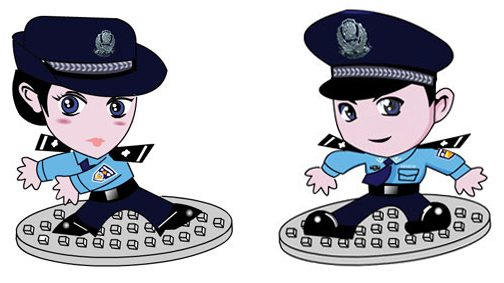
\includegraphics{figures/chap1/jingcha.jpg}
    \caption[Jingjing et Chacha, les policiers de l'Internet chinois]{\textit{Jingjing} et \textit{Chacha} sont deux figures créées par les autorités chinoises pour signifier la présence policière en ligne aux internautes. Le nom de ces veilleurs dessinés est une composition issue du mot “police” en chinois (\textit{jingcha}). Source : \url{http://jswm.newssc.org/system/2008/10/29/011233423.shtml} consultée le 17 Février 2014, à 15:32}
    \label{fig:jingcha}
\end{figure}

Au-delà de l’activité manuelle de milliers d’employés, GFW opère également plusieurs types de blocages sur les contenus. Techniquement, la plupart des filtrages se déroulent au niveau du fournisseur d’accès avec notamment des adresses particulières qui sont rendues inaccessibles : l’adresse \textit{facebook.com} ou \textit{youtube.com} renvoie une erreur “404 : Le site demandé n’existe pas”. Ainsi, de nombreux sites célèbres ne sont pas accessibles (\textit{Twitter}, \textit{Youtube}, \textit{Facebook}, etc.) Les autres blocages effectifs s’effectuent selon les adresses IP ou les serveurs d’attribution de noms de domaine (DNS) menant parfois au blocage de serveurs entiers \citep{Winter2012}. Les URLs des pages de certains sites importants sont également filtrées. Sur Wikipedia notamment, la page \textit{“Tiananmen Square protests of 1989”} est inaccessible depuis la Chine sans que le site Wikipedia soit pour autant intégralement bloqué. Également, des requêtes contenant des mots “interdits” sur les moteurs de recherche peuvent conduire à des micro-coupures ou un accès restreint au web pendant parfois plusieurs minutes\footnote{Testé depuis Shanghai en Septembre 2013.}. La liste des sites et mots bloqués n’est pas publiée par le gouvernement et l’ajout sur ses listes s’effectue a priori sur la demande de différentes agences gouvernementales chinoises, sans notification publique. Essentiellement, il s’agit de sites à caractère pornographique (la pornographie est illégale en Chine), de sites liés aux groupes dissidents chinois (Falung Gong, Dalai Lama, Tibet Libre...), de sites du gouvernement taiwanais et d’autres sites revendiquant la liberté d’expression pour la Chine\footnote{Si ces sites ne sont pas publiés officiellement, une liste est néanmoins maintenue par une entreprise privée sur le site http://www.greatfirewall.biz, consulté le 17 février 2014.}.

Si le GFW est un outil de contrôle politique, il participe également largement au protectorat économique chinois. L’expansion rapide du vaste marché de l'Internet en Chine s’est faite sous un strict contrôle politique et si l’État a largement financé les infrastructures, GFW a été l’un des moteurs de la croissance des grandes sociétés du web chinois. L'absence du géant \textit{YouTube} a notamment permis aux acteurs locaux de la vidéo en ligne de se développer rapidement. \textit{Youku}, son homogue chinois, est aujourd’hui sujet à une valorisation colossale sur les marchés d’affaires. La situation est similaire pour les réseaux sociaux. L'absence de concurrence étrangère due à l’interdiction de \textit{Facebook} en 2008 puis \textit{Twitter} en 2009 a permis aux acteurs chinois de se développer. Leur poids sur le marché intérieur les autorise aujourd’hui à rivaliser avec leurs concurrents américains au niveau mondial tant en nombre d’utilisateurs qu’en revenus directs et indirects générés \citep{CIW2012}.

Ainsi, GFW a affecté l’économie du pays en profondeur et à ce titre notamment continue d’être une préoccupation première du pouvoir politique. L’évolution technologique de GFW suit de près l’évolution des moyens de contournement des blocages, qui sont nombreux. Le célèbre logiciel \textit{Tor} garantissant l’anonymat sur Internet est aujourd’hui bloqué en Chine \citep{Winter2012} ainsi que d’autres technologies communes d’anonymisation (comme le proxy notamment). Pourtant, il reste très facile de \textit{``faire le mur''(fanqiang)} et d’accéder aux contenus en contournant les limites du GFW. Les solutions techniques à disposition sont multiples et souvent peu coûteuses à mettre en place ou à utiliser. De nombreux services commerciaux proposent de se connecter depuis d’autres pays à l’aide d’un VPN (\textit{Virtual Private Network}) pour un coût très faible. Le VPN permet d'accéder au Web depuis une machine située dans un autre pays et de bénéficier ainsi de l’accès tel qu’il existe dans le pays où se situe la machine. Le flou juridique qui entoure l’existence de services commerciaux de contournement de GFW témoigne de l’intérêt du gouvernement chinois à protéger largement le marché intérieur en supprimant l’accès aux services majoritaires du web occidental, sans pour autant exercer une traque systématique de chaque personne voulant utiliser \textit{Facebook} ou \textit{Gmail}. De plus, l’absence totale de moyens de contournement interdirait l’accès à des sources précieuses d’informations professionnelles (notamment \textit{Twitter}). Les autorités chinoises ne semblent pas prêt à payer le prix de cette perte d’avantages concurrentiels décisifs pour les entreprises chinoises. Une étude de l’OpenITP parue en 2013 analyse l’usage des outils de contournement de la censure auprès d’un échantillon de 1175 utilisateurs en Chine. Au-delà des solutions technologiques variées, on peut noter que la première raison pour contourner le blocage de l’Internet est l’utilisation des services de \textit{Google} (notamment de \textit{Gmail})\footnote{Bloqué en Chine, testé en Juin 2014 à Shanghai et Shenzhen}, suivi de la volonté de se rendre sur les sites de réseaux sociaux américains comme \textit{Facebook} et \textit{Twitter}, puis de l’accès aux contenus d’actualité, de vidéo en ligne et de sites à caractère pornographique. Les utilisateurs souhaitant accéder à des contenus à caractère politique ou utilisant l’Internet de manière anonyme pour communiquer de façon plus sécurisée représentent moins de 10\% de la population étudiée \citep{OpenITP2013}. Il est également important de noter que l’immense majorité des internautes chinois n’utilise pas de système de contournement des blocages de l’Internet. 

\section[Médias sociaux en Chine : un paysage morcelé]{Médias sociaux en Chine : un paysage morcelé}

Alors qu’un blocage officiel s’applique sur les plus célèbres sites Internet californiens, de nombreux services se sont développés pour répondre aux besoins et intérêts des internautes chinois. Cette culture particulière des entreprises politiques et économiques du web chinois influe sur l’être-ensemble des usagers et les contenus diffusés sur le réseau.

Profitant de l’absence des grands noms du réseau social en ligne, de nombreux services ont vu le jour sur la Toile chinoise. L'importance du \textit{guanxi} \citep{Yu2008}, élément profond de la culture traditionnelle poussant chaque Chinois à entretenir et exposer avec soin ses relations en société, peut également avoir contribué à créer un terrain idéal pour le développement rapide de ces sites \citep{Yang2011b}. Plutôt morcelé, le paysage des SNS en Chine offre une variété de services et d’acteurs qui rassemble les internautes chinois selon leurs centres d'intérêts. \textit{Douban} offre aux jeunes ``branchés'' de partager lectures, films et musique. \textit{Kaixin001}, plus centré sur les jeux, propose un espace ludique pour les trentenaires au bureau. \textit{Renren} (anciennement \textit{Xiaonei}) est, quant à lui, un véritable clone de \textit{Facebook} et se focalise sur le monde étudiant chinois \citep{Renaud2011}. Malgré ces nombreux concurrents, le service de messagerie instantanée \textit{QQ} reste le leader incontesté du marché chinois. Aujourd’hui classé 8ème site le plus visité au monde\footnote{D’après Alexa.com, consulté le 3 Février 2013.}, \textit{QQ} dénombre jusqu’à 100 millions d’utilisateurs connectés simultanément\footnote{Voir \url{http://im.qq.com/culture}, consulté le 14 Février 2013.}. Quatrième plus grande firme du web mondial, son créateur le géant \textit{Tencent Holdings Limited} a investi depuis le début de l’Internet en Chine dans de nombreux domaines des TIC : jeux, publicité en ligne, e-commerce, etc. Plus qu’une simple messagerie de chat, les services de \textit{QQ} sont multiples : la page de profil de chaque utilisateur (\textit{QZone}) permet de maintenir un blog et d’écouter de la musique (\textit{QQmusic}). Chaque utilisateur peut se créer un avatar en ligne pouvant revêtir de nombreux vêtements et accessoires vendus en ligne (\textit{QQshow}) mais aussi participer à de nombreux jeux multi-joueurs pour tous les âges (\textit{QQ Entertainement}). Le système de monnaie virtuelle (\textit{QCoin}) mis en place pour les achats en ligne a généré dès son lancement en 2005 un nombre important de transactions\footnote{\textit{Central Bank alert on ``virtual money''}, People’s Daily, 12 Janvier 2007, \url{http://english.people.com.cn/200701/12/eng20070112_340681.html} consulté le 28 Mai 2014}, poussant même \textit{Tencent} à obtenir une licence bancaire. L’utilisation de la messagerie \textit{QQ}, réseau social avant l’heure, est devenue un véritable phénomène de société porté par la diversification de \textit{Tencent} dans de multiples secteurs sous une marque unique. Au-delà des jeunes et des professionnels de l’Internet, le réseau \textit{QQ} comptait en juillet 2011 plus de 812,3 millions de comptes actifs, faisant de lui le deuxième réseau social mondial après \textit{Facebook}. Du magasin de photocopie de quartier au réseau de prostitution clandestin, \textit{QQ} héberge les discussions quotidiennes et fait pour ainsi dire partie intégrante du paysage des villes modernes. Les chinois échangent plus volontiers leurs numéros de \textit{QQ} que ceux de leurs téléphones portables et ce mode de communication est souvent préféré au mail dans les échanges au bureau. Convergeant rapidement avec la croissance fulgurante du e-commerce en Chine, les produits dérivés estampillés \textit{QQ} sont devenus une véritable mode en Chine : voitures, téléphones, boissons, etc. Le groupe \textit{Tencent} poursuit son évolution avec le lancement en 2008 de son service de microblog \textit{Tencent Weibo}, qui a connu un véritable succès dès les premiers mois. Aujourd’hui, la firme de Shenzhen continue la conversion de ces utilisateurs \textit{QQ} vers sa plate-forme mobile \textit{WeChat} qui connaît actuellement une très forte croissance, au point de voir les autres services de microblog mis au banc par les utilisateurs. Messagerie écrite et vocale, \textit{WeChat} se diversifie en offrant désormais d’utiliser son compte \textit{QQ} comme moyen de paiement pour de nombreux services du quotidien (taxis, nourritures, etc.)\footnote{\textit{21 million taxi rides have been booked on WeChat in the past month}, Tech in Asia February 12, 2014 \url{http://www.techinasia.com/wechat-21-million-taxi-rides-booked} consulté le 17 Février 2014 à 15:36}.

\subsection[Microblog en Chine et Sina Weibo]{Microblog en Chine et Sina Weibo}
Les sites de \textit{microblogging} (en chinois \textit{weibo}) permettent aux utilisateurs de poster de courts messages composés de photos ou de texte de 140 caractères maximum, puis de les commenter et de les partager avec leurs lecteurs. A l’image de \textit{Twitter}, chaque utilisateur peut souscrire aux fils d’info d’autres utilisateurs afin de recevoir leurs messages et mises à jour.

L’histoire du microblog en Chine débute en 2007 avec plusieurs services se présentant alors comme des clones de \textit{Twitter}. Le service \textit{Fanfou} connait notamment un succès rapide. De nombreux journalistes l’utilisent pour enquêter et coordonner leurs actions lors de l’arrivée du SRAS ou le tremblement de terre de Wenchuan dans le Sichuan en 2008. \textit{Fanfou} est fermé sur ordre du gouvernement en juillet 2009, suite aux nombreux commentaires suscités par des émeutes s’étant déroulées à Urumqi dans la province du Xinjiang. A peine un mois après cette fermeture, la firme \textit{SINA Corporation} saisit l’opportunité et s’installe en lançant son propre service de microblog intitulé \textit{Sina Weibo}. \textit{Sina Weibo} connaît dès son lancement une croissante soutenue avec plus de 10 millions de nouveaux inscrits par mois et devient en 2012 la plateforme de microblog la plus utilisée en Chine avec 250 millions d’utilisateurs \citep{McKinsey2012}. Les revenus de \textit{Sina Weibo} ne cessent alors de croître (+19\% en 2012\footnote{Voir \url{http://corp.sina.com.cn/chn/Annual_Report_2011_Final.pdf}, consulté le 16/02/2013.}) alors que plus de 86 millions de messages sont postés chaque jour sur ce service\footnote{D’après Sina Corp. Earning Calls - \url{http://phx.corporate-ir.net/phoenix.zhtml?c=121288&p=irol-EventDetails&EventId=4727394}, consulté le 16/02/2013}. 


\begin{figure}[htbp]
    \centering
    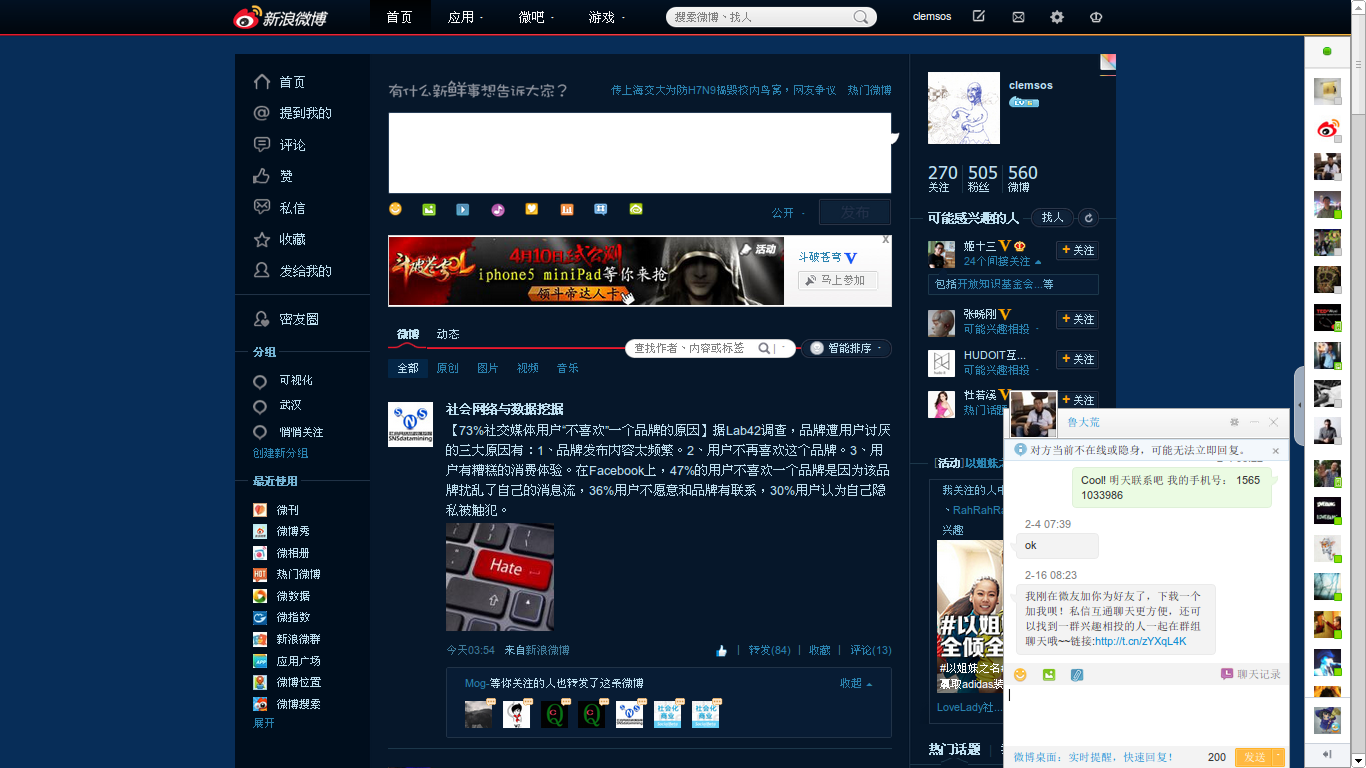
\includegraphics[scale=0.3]{figures/chap1/screenshot.png}
    \caption[Capture d’écran de Sina Weibo]{Capture d’écran de Sina Weibo, réalisé le 9 Avril 2013 à 08:59}
    \label{fig:screenshot_weibo}
\end{figure}

Figure historique de l’Internet chinois, \textit{SINA Corporation} est célèbre pour son portail \url{sina.net} et son immense plate-forme de blogs qui en font le fleuron des fournisseurs de contenus en ligne en Chine. Spécialisée dans ``l’infotainment'' (un mélange très tabloïd d’actualité et de news people), \textit{SINA} est la première compagnie nationale chinoise à avoir été listée au \textit{NASDAQ} dès Avril 2000. Avec son \textit{Weibo}, la firme réussit un coup de force commercial et prouve une fois encore combien la censure gouvernementale est bénéfique à l’industrie du web chinois. Néanmoins, la réussite de \textit{SINA} et de son service de microblog ne se fait pas sans connaître de nombreux ajustements parfois chaotiques. En effet, la stratégie agressive d’acquisition d’audience soutenant la croissance de \textit{Sina Weibo} offre pour garantie aux utilisateurs de pouvoir mieux s’informer et discuter plus facilement en ligne. Dès le début de l’année 2010, les suppressions de comptes utilisateurs et de messages non désirés commencent à se répandre dans le service. Les discussions politiques sont régulièrement effacées et \textit{Sina} se voit contraint de mettre en place un système de censure efficace sous la pression du gouvernement de Pékin. Néanmoins, afin de continuer à garantir la croissance du service, la firme de Pékin laisse une relative liberté aux utilisateurs en étant plutôt souple sur la surveillance des discussions et les actions prises. Des personnalités publiques ou journalistes devenues “weibo-stars” mobilisent régulièrement l’opinion publique autour de sujets d’actualité, attirant souvent des millions de lecteurs et de commentaires. Plusieurs scandales éclatent en ligne, mettant en cause des officiels et leur famille\footnote{Le fils d’un haut-cadre du Parti, arrêté ivre par la police après avoir renversé 5 personnes, annonce : \textit{”Mon père s’appelle Li Gang”} et se voit immédiatement libéré. Cette impunité provoquera un tollé chez les internautes \url{http://www.chinadaily.com.cn/china/2011-03/02/content_12099500.htm}}. Le 23 Juillet 2011, deux trains déraillent sur la ligne reliant Ningbo à Wenzhou inaugurée en fanfare quelques jours auparavant, faisant près de 40 morts et quelques 200 blessés. La colère gronde alors que le gouvernement tarde pendant plusieurs jours à prendre la parole sur ce sujet d’actualité épineux. Sur la toile et \textit{Sina Weibo} en particulier, les discussions vont bon train et les internautes indignés commentent le dernier drame du développement trop rapide de la Chine, où se mêlent détournement de fonds, corruption et sécurité publique. 


\begin{figure}[htbp]
    \centering
    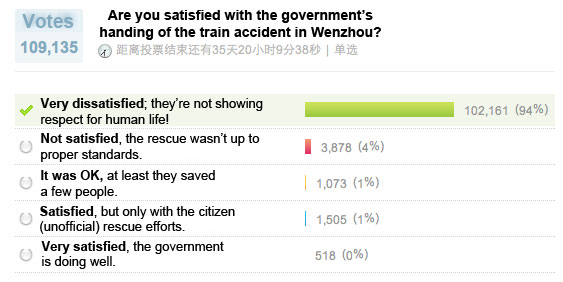
\includegraphics[scale=0.7]{figures/chap1/train.jpg}
    \caption[Sondage Weibo concernant l'accident de train de Wenzhou]{Un sondage publié sur \textit{Sina Weibo} (traduction C. Custer, Tech in Asia, 1er Aout 2011), consulté le 24 Février 2014, à 22h12.}
    \label{fig:poll_weibo}
\end{figure}

\textit{Sina Weibo} désactive alors la fonction de commentaires des messages. Dans les jours suivants, le gouvernement fait enfin une déclaration officielle sur les causes de l’accident de train puis se décide à agir en mettant en garde les internautes trop audacieux de représailles à venir. Les messages controversés sont supprimés, plusieurs comptes utilisateurs sont fermés, la police convoque les meneurs des discussions et d’autres mesures d’intimidation sont menées auprès des journalistes et des weibo-stars qui se seraient exprimées un peu trop directement à l’égard du Parti. Dans le même temps, le gouvernement a du mal à se saisir de ce nouvel outil. Alors que les administrations locales, universités et les médias d’État ont plutôt bien réussi le virage de leur stratégie de communication vers le microblog, les membres du gouvernement de Pékin ouvrent des comptes où ils sont parfois raillés, tournés en ridicule et harassés de questions. En Février 2012, les quatre plus grosses sociétés de microblog (dont \textit{Sina Weibo}) annoncent que chaque utilisateur est maintenant contraint de modifier son profil pour mentionner son véritable nom, prénom ainsi que son numéro de carte d’identité. Cette velléité de vérification échoue et est abandonnée quelques semaines plus tard face à la mobilisation des utilisateurs et la difficulté de faire appliquer de telles mesures. Le gouvernement de Pékin édite pourtant une série de règles \textit{“Several Regulations on Microblog Development and Administration Enacted by the Beijing Government”} dont la plus notable sera la possibilité de condamner tous ceux qui auront participé à la diffusion d’informations considérées comme fausses, erronées ou mensongères. Face à la multiplication des actions gouvernementales et à l’apparition d’autres plate-formes, la croissance du nombre d’utilisateurs de \textit{Sina Weibo} est désormais stoppée pour aborder une phase de déclin estimé à près de 10\% dans les deux premiers mois de 2014\footnote{D’après le CNNIC cité dans l’article  \textit{“China’s Twitter is bleeding users”}, 17 Janvier 2014, \url{http://blogs.marketwatch.com/thetell/2014/01/17/chinas-twitter-is-bleeding-users}, consulté le 17 Février 2014 à 18:17}. 

\begin{figure}[htbp]
    \centering
    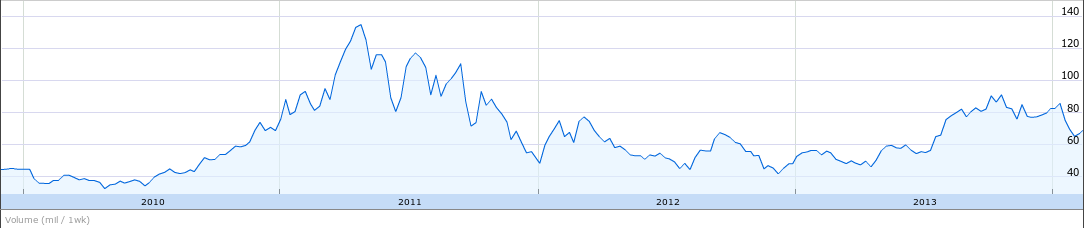
\includegraphics[scale=0.4]{figures/chap1/sina.png}
    \caption[Cours de l’action SINA au Nasdaq entre 2009 et Février 2014]{Cours de l’action \textit{SINA} au Nasdaq entre 2009 et Février 2014 - Source : \textit{Google Finance}, consulté le 17 Février 2014 à 15:28 }
    \label{fig:sina_nasdaq}
\end{figure}

A la lecture de l’histoire de \textit{Sina Weibo} on constate l’ambivalence des actions officielles du gouvernement chinois dans la réussite économique des entreprises d’Internet. Si la firme \textit{SINA} a bénéficié de prime abord d’un avantage compétitif notoire par l’élimination de la concurrence, elle a par la suite souffert des conséquences du contrôle politique de l’Internet, avec notamment une perte de ses utilisateurs.


\subsection[Sina Weibo, un usage plus ludique que \textit{Twitter} ]{Sina Weibo, un usage plus ludique que \textit{Twitter} }

Dans son article nommé \textit{A Tale of two microblogs}, Jon L. \cite{Sullivan2012} raconte comment l’événement historique de la fermeture de \textit{Twitter} en Chine a vu la communautés des microbloggers chinois se scinder en plusieurs groupes distincts : 

\begin{itemize}
\item \textit{Twitter} rassemble une communauté avide de libres discussions, souvent très politisées voire radicalement en opposition avec le gouvernement chinois.
\item \textit{Tencent Weibo} est utilisé par les utilisateurs de \textit{QQ}, typiquement des personnes aux revenus plus faibles accédant au web depuis leurs mobiles.
\item \textit{Sina Weibo} est le favori des travailleurs urbains, souvent plus jeunes ou éduqués, représentant davantage la classe moyenne montante.
\end{itemize}

Dans la littérature en sciences informatiques, plusieurs articles proposent des comparaisons entre \textit{Twitter} et \textit{Sina Weibo}. Une large analyse quantitative et comparative menée avec des jeux de données des deux services \citep{Gao2012} nous apprend que le contenu de \textit{Sina Weibo} est davantage corrélé avec des sentiments positifs (analysés automatiquement). Les utilisateurs de \textit{Sina Weibo} parlent davantage de lieux et de personnes alors que les utilisateurs actifs sur \textit{Twitter} s’intéressent plus aux organisations. Également, \textit{Sina Weibo} connaît un pic d’activité le week-end alors que \textit{Twitter} affiche généralement une baisse de régime dans les fins de semaine. Ces différentes indications suggèrent que \textit{Sina Weibo} serait davantage utilisé pour des activités de loisir quand \textit{Twitter} se destinerait à un usage plus professionnel. Une étude s’intéressant aux tendances sur \textit{Sina Weibo} \citep{Yu2011} indique que la majorité des comptes les plus influents de \textit{Twitter} ont été vérifiés contrairement à \textit{Weibo} où le taux est plus faible chez les grands utilisateurs. La vérification d’un compte se fait par l’authentification auprès du fournisseur de service afin d’attester l'identité de la personne utilisant le compte. C’est un enjeu important pour les figures publiques (marques, stars, hommes politiques, etc.) Cet indicateur nous montre donc l’intérêt professionnel fort entourant \textit{Twitter}, moins pressant dans le cas de \textit{Sina Weibo} où moins de personnes ont ressenti la nécessité de faire officialiser leurs comptes. Sur les deux services de microblog, les utilisateurs inscrits possèdent un réseau de relations identifiables par leur souscription aux fils d’infos d’autres utilisateurs (\textit{follow}). La relation peut être inexistante (\textit{none}), mutuelle (\textit{friend}) ou unidirectionnelle (\textit{follow}, un utilisateur suit un autre mais n’est pas suivi par ce dernier). La comparaison d’échantillons des graphes sociaux issus des deux services \citep{Chen2012} montre comment les relations sur \textit{Sina Weibo} sont plus dissymétriques et moins réciproques, reflétant une hiérarchie plus forte entre les utilisateurs que \textit{Twitter}. 

Un autre facteur important de différentiation entre les deux services est la nature de la diffusion des contenus postés sur \textit{Sina Weibo}. Contrairement à \textit{Twitter} où le texte domine, la majorité des posts de Weibo contiennent des images ou des vidéos \citep{Zhao2012}. Les posts possédant des contenus multimédia (images, vidéos...) sont plus susceptibles d’être diffusés largement et restent en moyenne actifs pour une durée plus longue \citep{Zhao2012}. Également, les contenus sur \textit{Sina Weibo} possèdent une proportion moins élevée de retweets et de commentaires que sur \textit{Twitter} \citep{Zhao2012, Gao2012}. L’activité de la population de \textit{Twitter} est plus intense, moins tournée vers la diffusion de masse et plus réactive aux influx de nouveaux contenus. 

Nous voyons donc que le paysage de \textit{Sina Weibo} se constitue autour de stars et célébrités concentrant l’attention avec des contenus à la diffusion très large. Moins tourné vers l’actualité et la conversation que son homologue \textit{Twitter}, \textit{Sina Weibo} agit comme véhicule de contenus à grande audience, souvent publiés par des personnalités publiques célèbres. Des études quantitatives montrent bien que les contenus les plus échangés et discutés concernent les loisirs et divertissements, la mode, la santé, etc. \citep{Li2013}. Les messages à caractère humoristique (texte, images et vidéos) occupent également une place prépondérante dans les échanges des utilisateurs, contrairement à son homologue américain \textit{Twitter} dominé plutôt par les sujets d’actualité \citep{Yu2011}. \textit{Sina} poursuit ainsi son rôle historique de leader chinois de \textit{l’infotainment}. 

Pourtant, la population de jeunes urbains qui soutient la croissance de son service de microblog reflète aussi les transformations en cours dans la société chinoise. Les journalistes et spécialistes de l’information sont les premiers à se saisir de ce nouveau média. Dans un discours à Stanford en 2013, le PDG de \textit{Sina} Charles Chao explique : 

\begin{quote}
\textit{Le plus grand changement apporté par le microblog en Chine concerne d’abord l’industrie des médias elle-même. Aujourd’hui, plus de 30\% des actualités ont d’abord été reportées sur \textit{Sina Weibo} avant d’atteindre les médias   traditionnels. Le rôle des médias traditionnels a été déplacé vers un traitement des informations en profondeur (in-depth reporting).} \footnote {Charles Chao, PDG de Sina pendant la Stanford Graduate School of Business China 2.0 tenue le 3 Octobre 2013. Disponible en vidéo \url{http://www.youtube.com/watch?v=tlliivJKHk8}, consultée le 19 Février 2014 à 11:23} (traduction de l’auteur)
\end{quote}

L’omniprésence des supports mobiles (smartphones, tablettes)\footnote{Selon l’Universal Telecommunication Union, \textit{``la Chine dépasse 1 milliard d’abonnements mobile, avec 400 millions d’utilisateurs d’Internet mobile dépasse ainsi les États-Unis comme leader du marché des smartphones''}, \url{http://mobithinking.com/blog/china-top-mobile-market} consulté le 24 Février 2012.} permet en effet des modes de traitement de l’information jusqu’ici inconnus qui bousculent les hiérarchies très contrôlées des salles de rédaction chinoises. Alors que la population urbaine croît rapidement, le smartphone est \textit{``the first big urban purchase''} \citep{Wallis2013} pour les nouveaux arrivants en ville et représente un outil indispensable de participation à la société. En 2008, la Chine était le seul pays en Asie où les moins de 30 ans possèdent plus d’amis en ligne que hors ligne \citep{Hinckley2009}. Ainsi, les réseaux sociaux jouent un rôle primordial dans la socialisation urbaine et viennent changer les modes d’expression. Le lectorat chinois a perdu toute confiance dans la plupart des médias traditionnels suite à l’absence répétée de courage et à la rétention d’informations cruciales dans les dossiers importants animant le pays. 

Le microblog s’installe comme une nouvelle source de confiance pour des millions de citoyens voulant comprendre et prendre part aux changements cruciaux de la société chinoise moderne. Un rapport de l’Institut de Journalisme Reuters à l’Université Oxford paru en 2013 montre comment les usages du microblog ont amené des transformations dans le quotidien des journalistes chinois. Le journalisme d’investigation a notamment connu un essor important grâce au renouvellement des sources et une large diffusion en ligne des sujets. \textit{Sina Weibo} n’a pas amélioré nécessairement la qualité de leurs investigations, mais a par contre permis une plus grande dissémination. Il est à noter que les spécificités de l’écriture chinoise rendent possible l’écriture d’un court texte en 140 caractères, alors qu’une telle longueur autorise seulement une courte phrase dans une écriture utilisant un alphabet latin. La mobilisation des utilisateurs pour la protection des journalistes a également joué un rôle important ainsi que le renforcement de procédés de vérification existant depuis longtemps sur les forums du web chinois. Très populaire dans les années 2000, Le \textit{``moteur de recherche de viande humaine''} (\textit{renrou sousuo}) est une forme de traque d’individus en ligne réalisée par un large nombre d’internautes à partir d’un nom ou d’une photo. Il s’agit souvent de retrouver quelqu’un désigné comme ``coupable'' (d’adultère, de corruption, etc) en réunissant un maximum d’informations à travers la Toile afin d’identifier ou de localiser la personne. Devant les dérapages rapides de ce type de procédés, les questions d’éthique sont au cœur des discussions qui entourent le journalisme en ligne. En effet, l’usage des médias sociaux a permis à certains journalistes de faire pression sur les pouvoirs publics, amenant parfois à la censure de leurs travaux, mais a également permis une très large auto-promotion pour de nombreux journalistes devenus des stars de \textit{Weibo}.

\begin{figure}[htbp]
    \centering
    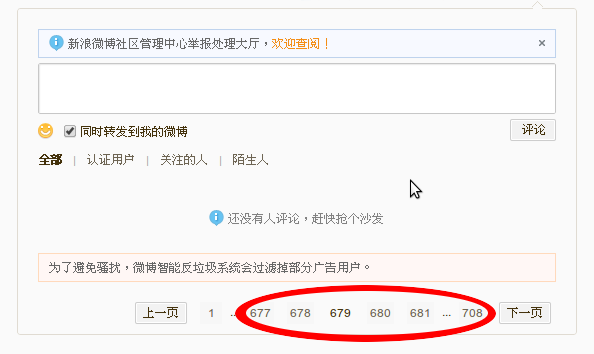
\includegraphics[scale=0.5]{figures/chap1/comments.png}
    \caption[Commentaires supprimés par Sina]{La trace des commentaires supprimés par Sina est encore visible - Page 677 à 708, les commentaires ont été supprimées, soit approximativement 4\% messages supprimés (589 messages sur 13452, à raison de 18 à 20 messages par page). Capture d’écran effectuée le 29 Janvier 2013 à 12:32:42, \url{http://www.weibo.com/1701401324/zeoBquVKi}, consulté le 16/02/2013.}
    \label{fig:comments}
\end{figure}

Le contrôle des contenus sur \textit{Weibo} est donc une réalité quotidienne et a été depuis son lancement la source de plusieurs études. Les formes les plus courantes sont : la suppression de posts, la suppression de comptes utilisateurs et le blocage de mots-clés. Le blocage de mots-clés s’effectue dans le moteur de recherche interne du site (“pas de résultats” quand vous cherchez un mot bloqué) et plus récemment par l’impossibilité de poster un message contenant des mots ou des adresses web bloqués \citep{Ng2013}. La pratique de la suppression de comptes s’est intensifiée en 2013\footnote{ \textit{“Over 100,000 \textit{Sina Weibo} Accounts Shut Down or Penalized for Govt Rules Violations”} par Gabriela Vatu, 14 November 2013 \url{http://news.softpedia.com/news/Over-100-000-Sina-Weibo-Accounts-Shut-Down-or-Penalized-for-Govt-Rules-Violations-400289.shtml} consulté le 17 Février à 16:42} avec notamment la suppression de millions de “zombies” présents sur le site. Les “zombies” sont des comptes utilisateurs créés par des robots dans le but de reposter automatiquement des contenus et d'augmenter le trafic sur le site. Les exigences des annonceurs publicitaires de plus en plus présents sur le site ont obligé \textit{Sina Weibo} à faire la chasse aux robots sur son site, faisant ainsi diminuer le nombre de comptes actifs de manière significative. La firme Sina est garante auprès du Ministère de la Sécurité Publique chinois des contenus qu’elle diffuse et effectue à ce titre une surveillance constante pour supprimer les messages “non-conformes”. Lors de nos recherches, nous avons constaté que l’interface de \textit{Sina Weibo} garde la trace des commentaires supprimés par le système d’administration. Dans les messages supprimés se trouvent à la fois des posts d’utilisateurs “zombies” et les posts jugés incorrects par les administrateurs. Au total, la suppression des messages s’effectue avec un taux estimé à environ 16\%, allant jusqu’à plus de 50\% dans certaines provinces comme Ningxia ou le Tibet contre seulement 12\% à Beijing \citep{Bamman2012}.


\section[Code, langage et milieu(x) numérique(s)]{ Code, langage et milieu(x) numérique(s)}

L’espace d’expression offert par l’Internet chinois et ses services de réseaux sociaux héberge donc une variété de pratiques, de questions et de réflexions qui nécessitent d’être appréhendées avec des outils de problématisation et d’analyse spécifiques. Dans la troisième et dernière partie de ce chapitre introductif, nous allons donc nous pencher sur les concepts existants dans la littérature scientifique sur l’existence \textit{in situ} des objets numériques. Afin de mettre en perspective le Web chinois et l’histoire de ces objets, nous introduirons notamment le concept de \textit{milieu numérique}, héritier de l’idée complexe de milieu que nous explorons ci-après.

\subsection[Lieu, espace, territoire et technologies]{Lieu, espace, territoire et technologies}
Géographie, management et diffusion de l’innovation, histoire des technologies, \textit{cultural studies} ou études “nationales”, les travaux qui s’intéressent aux relations entre technologies, espace, lieux et territoires sont nombreux et offrent un paysage riche où se croisent de nombreuses disciplines scientifiques. L’influence des réseaux de transports sur l’expérience humaine et le développement des villes a notamment été largement étudiée \citep{Offner1993,Doulet2001}. L’Internet a également fait l’objet de nombreuses études monographique (par pays) ou comparative, une étude à l’échelle mondiale présentant en effet des problèmes de données et évidemment d’échelle \citep{Dupuy2004}. En Chine où l'urbanisation produit actuellement une vaste migration des ruraux vers la ville, l'utilisation des réseaux sociaux médiatise bien souvent les choix de lieux et les rencontres des nouveaux arrivants. De nombreux groupes de discussions réunissent par exemple les nouveaux acheteurs d’immobilier qui échangent leurs stratégies d’achat et de défense de leurs droits et de leurs biens \citep{Li2013}. L’usage des réseaux sociaux revêt pour les nouveaux arrivants une importance capitale, notamment dans la recherche de groupes similaires et l’échange d’expériences. A travers le navigateur, ils s'approprient la ville étrangère pour s'en construire peu à peu une représentation à leur image.

La carte notamment joue sur le web un rôle important d’abord en tant qu’illustration, puis plus récemment d’interface avec le réel. Loin d’être figée par le territoire, la carte le décrit sous un ou des angles particuliers \citep{Brunet1987, Jacob1992}. Le développement de standards comme le système GPS \citep{Haklay2008} et de services et outils de cartographie ont contribué à une appropriation de la pratique cartographique par un nombre croissant de personnes \citep{Crampton2009}. De nouvelles formes de données produites par les utilisateurs parfois appelées \textit{``volunteered geographic information''} \citep{Elwood2008} utilisent les services en ligne comme Google Maps pour dessiner un \textit{``miroir du monde offline''} \citep{Graham2011}. Le courant dit de la néogéographie fait usage du GIS et des outils en ligne (Google Maps, Flickr, etc.) pour comprendre les pratiques de ces nouvelles formes de \textit{``géographies volontaires''} \citep{Turner2006}. Ce rôle croissant de la cartographie dans l’usage d’Internet produit un \textit{``Geoweb''} constitué de données et métadonnées spatiales \citep{Crampton2009}. Le point d'entrée unique qu'offre le marqueur spatial (\textit{geotag}) réunit souvent de vastes quantités de données disparates: Open Data territorial, géo-localisation, GIS, POI\footnote{GIS : Geographic Information System ; POI : Point-Of-Interest}, etc. \citep{Torrens2010}. Cette présence accrue dans le réseau dessine l’enjeu non seulement de cartographier le monde, mais également de cartographier le réseau lui-même, ouvrant ainsi de nouvelles voies pour découvrir la construction sociale des espaces par des pratiques individuelles et de groupe. Dans cette étude, nous avons donc choisi d’interroger les objets numériques afin de comprendre comment se structurent la parole et la conversation dans le contexte unique de l’Internet chinois. Afin d’articuler les multiples dimensions d’analyse qui viennent enrichir notre réflexion, il nous faut donc brosser un portrait en large de l’Internet chinois, en le considérant tour à tour comme un \textit{espace} structurant pour les actions des internautes qui le pratiquent, comme un \textit{territoire} sujet aux relations de pouvoir actualisées par les groupes et individus et enfin comme un \textit{lieu} habité par ceux qui y construisent chaque jour des significations communes. Nous proposons ici une revue sélective des quelques travaux à même de nous apporter des éclairages pertinents dans la vaste littérature s’intéressant aux dimensions géographiques des TIC.

\subsubsection[Code / space : l’espace transductif des TIC]{Code / space : l’espace transductif des TIC}

Dans leurs recherches autour de la géographie des technologies numériques, Dodge \& Kitchin ont travaillé à développer le concept de code comme un élément fondateur des espaces modernes dans lesquels nous évoluons. Reflétant l’importance croissante accordée aux TIC dans l’environnement urbain, ils citent un travail sur la production automatique des espaces : \textit{“De plus en plus, les espaces de la vie  quotidienne nous parviennent chargés de logiciels (software)”} \citep{Thrift2002} En effet, si le projet urbain a été guidé pendant le demi-siècle dernier par l’apparition de la technologie automobile dans l’espace des rues, les TIC paraissent prendre le relais avec l’idée d’une ville intelligente et connectée, connue sous le nom de \textit{`` smart city ''} \citep{Ascher2009,Picon2014}. Dodge \& Kitchin ont donc fait du \textit{code} une des pierres d’angles de l’appréhension de l’espace dans leur travail en le définissant comme suit : 

\begin{quote}
\textit{``an instruction or rule that has a single outcome determined by a binary logic (yes/no). The combination of these indidivuals logic rules produces code (program).''} \citep{Kitchin2011}.
\end{quote}

La part croissante des TIC dans nos espaces quotidiens amène les auteurs à envisager l’espace dans son interaction avec le code, symbolisant la suite d’instructions machiniques et électroniques qui permettent à un espace de remplir sa fonction. Dans un article intitulé \textit{Flying through code/space: the real virtuality of air travel}, Dodge \& Kitchin analysent la structure des espaces aéroportuaires. De l’achat des tickets jusqu’au vol des avions en passant par la gestion des bagages, le bon fonctionnement d’un aéroport est entièrement régi par les longues successions d’instructions du code. Ici, Dodge et Kitchin proposent le concept de code/space pour décrire ce type d’espace spécifique où lorsque le code échoue (\textit{failure}) alors le code/space tout entier échoue \citep{Dodge2004}. L’exemple de l’aéroport est parlant : si le système de check-in des bagages ou les machines responsables du contrôle de sécurité des passagers ne fonctionnent pas, alors l’espace aéroportuaire ne peut exister en tant qu’aéroport. L’analyse de la spatialité ne se situe alors plus dans un domaine sémantique ou narratif, mais plutôt dans les processus et opérations qui s’y déroulent et le code et les technologies y jouent un rôle primordial : 

\begin{quote}
    \textit{``Code is employed as the solution to a problem, a particular kind of transduction  is occurring.''} \citep{Kitchin2011}. 
\end{quote}

L’espace n’est pas un donné mais s’explique plutôt comme : \textit{``une forme d’ontogenèse (en perpétuel devenir-au-monde), l’espace est une pratique; un faire ; un événement (…) qui ne pré-existe pas à son faire (doing)''} \citep{Kitchin2011}. L’espace est considéré non pas comme une production, mais comme une \textit{transduction}. Reprenant le travail de Simondon sur l’individuation par la technologie, Dodge et Kitchin présentent l’espace comme une pratique qui comprend les actes, actions, occurrences, mémoires, perceptions, etc. d’un groupe d’individus s’y trouvant. La fonction de l’espace est structurée par les individus et le code y est considéré comme une entité agissante. Dans le \textit{code/space}, la relation dyadique entre code et espace est bijective: l’un ne peut aller sans l’autre. En terme simondonnien, la transduction ne peut être assurée sans code. Si l’exemple de l’aéroport illustre bien cette nécessité du code dans le devenir-espace, Dodge et Kitchin ont également identifié d’autres catégories où cette relation est plus ténue : les \textit{coded spaces}, qui peuvent poursuivre leurs fonctions même lorsque le code échoue ; les \textit{background coded spaces} où les processus de transduction induis par l’espace ne s’appuient pas nécessairement sur le code, mais proposent néanmoins des possibilités de l’activer (machine éteintes ou inactives, etc.) 

L’analyse fonctionnelle des rapports entre espace et technologie de Dodge \&Kitchin montre comment les TIC peuvent être un facteur \textit{transductif} pour les individus se mouvant dans les espaces de leurs vies quotidiennes. Si nous appuyons pleinement ce constat, il nous semble que le parti-pris des auteurs de considérer le “code” comme une abstraction incluant uniquement les instructions ou “logiques machiniques“ ferme la porte à l’immense densité des activités symboliques qui se jouent dans l’usage des technologies. Comment notamment considérer les “contenus” du web dans cette grille de lecture? Comment resituer dans une perspective historique les logiques de médiation de l’espace par les technologies de l’écriture? Il nous semble en effet que la faillite fonctionnelle (\textit{failure}) des code/space précède l’arrivée des technologies et s’opère déjà à un niveau symbolique - la fonction de l’espace du Palais du Louvre après la chute des rois de France se voit radicalement modifiée. La transduction opérée lors de la pratique d’un espace s’effectue dans un jeu d’appropriation symbolique qui passe notamment mais pas seulement par les technologies. Les technologies du langage et de l’information jouent notamment un rôle crucial dans l’affirmation du récit symbolique (\textit{narrative}) qui construit l’espace. L’activité du code dans la structuration des code/space de Dodge \&  Kitchin existe sous une forme non seulement fonctionnelle mais également sémantique, voire phatique ou même esthétique comme l’a décrite Jakobson dans ces analyses des fonctions du langage \citep{Jakobson1956}. Au-delà de sa dimension machinique, le code possède les caractéristiques d’une \textit{poiesis} dépassant l’idée simple de fonctionnalité pour exister dans la complexité d’une écriture comme traduction du langage humain et machine.

\subsubsection[Codes, discours et territoires des technologies]{Codes, discours et territoires des technologies}

Le code serait davantage à comprendre comme un mode d’expression humain à travers la technologie, actualisant l’\textit{épistémè} décrit par Foucault dans \textit{Les Mots et Les Choses} comme élément fondamental de la pensée d’une époque et sa considération pour le monde \citep{Foucault1996}. Ètat des connaissances scientifiques et littéraires, l'épistémè existe comme somme des savoirs d’une époque, présupposée traduite en un regard sur le monde. Le \textit{code} exprime les savoirs d’aujourd’hui dans de nombreux langages écrits. Le code source d’une page Internet, d’un programme informatique ou d’un driver hardware ne s’écrit pas seulement en langage ``machine'' mais fait appel à plusieurs langages informatiques et humains. A la fois production savante, outil scientifique, vecteur d’expression et interfaces des savoirs, le code constitue l’expérience narrative du monde par les TIC. Possédant de nombreux mots, aspects et syntaxes issus de multiples langues humaines, les replis de l’écriture informatique laissent transparaître de tout bord leur origine littéraire. L'alphabet se voit augmenté de nombreux caractères qui le rendent compatible avec l’encodage des bases de données - pensons à l’Unicode notamment \citep{Guichard2014}. Rappel à l'ordre, l'arrêt soudain de l’ordinateur ou la perte d’un fichier nous laisse frappés d’illettrisme. Seuls une minorité de personnes ``lettrées'' de l’informatique peuvent déchiffrer et comprendre le ``bug''. Ainsi, la définition du ``code'' de Dodge \&  Kitchin doit être étendue pour recouvrir plus largement les pratiques symboliques liées aux activités de l’écriture du code dans ces espaces.


Le code ainsi redéfini nous ramène alors à une lecture foucaldienne du discours dans sa relation intime avec le territoire \citep{Foucault2004}. Dans ces nombreux travaux sur la généalogie, Michel Foucault cherche à comprendre comment les relations de pouvoir créées par les discours portés sur les objets président à la production de territoires et d’interdits comme autant de sujets de ces discours. Nous définissons la \textit{discursivité} comme le processus de construction de ces discours. Historiquement, l’Internet a été très tôt sujet à l’appropriation par le discours de nombreux groupes actifs dans une volonté de territorialisation. La métaphore géographique et spatiale a structuré le vocabulaire de l’Internet dès sa création \citep{Graham1998}: site, cyberspace, etc. L’\textit{Electronic Frontier Foundation} se charge de protéger l’u-topie qu’est Internet avec sa fameuse \textit{Déclaration d’Indépendance du Cyberespace} \citep{Barlow2001}. A l’opposé du spectre, les autoroutes de l’information in-forment le paysage comme autant de géogrammes massifs \citep{Berque1999}. L’appropriation des protocoles du réseau, notamment par la lutte pour le respect de standards ouverts ou partagés, s’ancre également dans les pratiques du discours. Les mots \textit{free} et \textit{open} cristallisent l’histoire des revendication territoriales de l’Internet \citep{Blondeau2000}. L’autre grande métaphore constitutive de l’Internet est textuelle avec ses pages, langages et hypertextes \citep{Vandendorpe1999}. La formule choc \textit{``Code is law''} \citep{Lessig2006} résume l’idée  que les processus textuels du code mettent en jeu un ensemble de rôles, protocoles et mises en scène qui agissent comme autant d’autorités à travers le discours. La jurisprudence fait loi, comme écrit sur les murs des bureaux de \textit{Facebook} à Palo-Alto : \textit{``Code wins arguments''} \footnote{Dans la Lettres aux Investisseurs écrite par M. Zuckerberg  pour l’IPO de \textit{Facebook} \url{http://www.sec.gov/Archives/edgar/data/1326801/000119312512034517/d287954ds1.htm\#toc287954_10}}. La territorialisation de l’Internet se fait ainsi au travers d’un ensemble de pratiques discursives, méta-grammaire des discours en ligne. La confrontation symbolique au sein des territoires numériques se poursuit dans le discours, réifié dans les pratiques du code.

Sur l’Internet chinois, les pratiques de censure de l’écriture en sont le reflet le plus frappant. Blocage de mots-clés, détournements de langage, suppression et modification de texte sont l’expression de cet affrontement de discursivités parfois antagonistes. La Grande Muraille gouvernementale scanne les masses de texte pour reconnaître et stopper des mots tels que \textit{``Printemps arabe''} ou \textit{``évènements de Tian-An Men''} \citep{MacKinnon2012}. Néanmoins, l’état actuel des techniques de \textit{data mining} ne permet pas encore de déceler les phénomènes langagiers comme les jeux de mots ou l’ironie. Bien souvent, les internautes chinois choisissent l’humour pour permettre à leurs idées de se frayer un chemin. Revêtant leurs masques de chat, les internautes chinois sont devenus spécialistes dans la publication de jeux de mots, chansonnettes et petites vidéos d’animaux, comme autant de couperets cinglants pour railler les officiels trop pompeux de Pékin. Dans la guerre de l’information que se livrent sans cesse censeurs et internautes, de simples photos truquées de crabes et de lamas peuvent devenir héroïques. Ces blagues numériques, d’apparence inoffensive, font chaque jour le tour de la Toile chinoise, portant en elles toute la subversion d’internautes aspirant à plus de liberté. Début 2010, alors que pleuvaient les longs discours pieux du Parti sur l’harmonie de la nouvelle société (en chinois \textit{hexie}), on voit apparaître en ligne des essaims de crabes de rivière (se prononçant également \textit{hexie}) couverts de chaînes en or criant : \textit{“Vive l’harmonie”} au volant de leur limousine. Devenus aujourd’hui une image de la corruption des hauts dignitaires du Parti, on croise régulièrement dans les commentaires d’un article officiel un petit crabe de rivière, tel un rapide rappel posté par un lecteur.


\begin{figure}[htbp]
    \centering
    \subfloat[(hexie) : Harmonie / Discours du PCC sur l’harmonie]{ 
        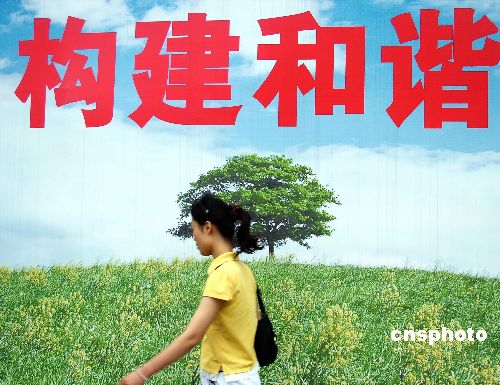
\includegraphics[scale=0.37]{figures/chap1/hexie2.jpg} 
    }
    \subfloat[(hexie) : Crabe de rivère / Mème satirique]{ 
        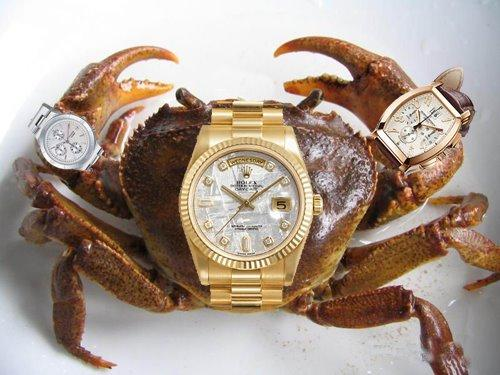
\includegraphics[scale=0.37]{figures/chap1/hexie.jpg} 
    }
    \caption[Hexie, les crabes de rivières]{ \zh{和谐} VS \zh{河蟹} - Mot de la semaine : Crabe de Rivière - China Digital Times du 21 Mars 2012 - Licence Creative Commons \url{http://chinadigitaltimes.net/2012/03/word-of-the-week-river-crab}, consulté le 15 Février 2013.}

\label{fig:hexie}
\end{figure}

On voit bien comment le code décrit un territoire sujet à l’autorité politique sous la forme d’un système de \textit{data mining} cherchant à mettre en forme le discours. La fonction du \textit{code/space} sémantique que forme ici l’espace de l’Internet est réécrit par un jeu de langage. La circulation d’objets digitaux permet de reterritorialiser cet espace en apparence régi par un code strict de censure. 

\subsubsection{Les lieux des technologies}
Dans son célèbre livre sur les Arts de Faire, \cite{Certeau1980} considère la ville comme un texte dont chaque piéton énonce et révèle (\textit{performe}) des sens nouveaux par son activité de marcheur. Actualisant l’espace urbain par sa marche, l’habitant de la ville s’approprie des lieux restant néanmoins partagés avec d’autres. Au détour des rues, le sens commun des lieux urbains se construit avec les multiples énonciations de ceux qui les habitent et les font vivre. Cette magnifique image de la poésie du texte urbain met en lumière la dualité que nous avons abordée précédemment : l’espace ne peut fonctionner sans les pratiques de ses habitants. Plus encore, l’être-ensemble et le devenir-soi procèdent de la construction de lieux communs, \textit{poiesis} des espaces habités. Les TIC font aujourd’hui souvent partie intégrante des lieux que nous habitons. \cite{Graham1998} dans son travail sur l’étude des lieux et de leur rapport à la technologie identifie trois types majeurs d’approches dans la littérature :


\begin{enumerate}

\item L’approche \textit{``substitutive''} ou \textit{``transductive''} qui voit dans l’arrivée des TIC la disparition de la valeur des lieux : un idéal de proximité utopique \citep{McLuhan1962} ou un discours dystopique sur leur proche disparition \citep{Virilio1998, Auge1995}. Ces considérations sont les formes traditionnelles du débat accompagnant l’innovation dont sont férus la communication industrielle et la critique des médias \citep{Ramonet2001}, restant souvent purement prospectif et faisant peu de cas des usages.

\item Plus modérée, l’approche qualifiée par Graham de \textit{``co-évolutionniste''} s’interroge sur la façon dont les interactions dynamiques des espaces virtuels (\textit{space of flows}) et réels (\textit{space of places}) \citep{Castells2009} produisent de nouveaux lieux . Ces études économiques et sociales prennent la forme d’une médiologie de l’espace adaptée aux études stratégiques pour l’urbanisme et l’implantation des télécommunications. Son interprétation par les aménageurs lui donne parfois une dimension déterministe peu utile à la compréhension des phénomènes liés à l’appropriation et l’historicité des technologies \citep{Offner1993}.

\item Une dernière approche plus récente se cristallise autour de l’idée de relations et de réseaux. Afin d’éviter l’écueil des causalités directes et de la notion fataliste d’impact, les lieux sont présentés comme \textit{`` des moments articulés dans un réseau de sens et de relation sociales ''} \citep{Massey1993}, des assemblages entre objets matériels “actants” \citep{Latour1996}, individus et groupes sociaux. Cette approche s’intéresse davantage au lieu comme une géométrie sociale en mouvement, liée au temps et à la situation \citep{May2001} et refuse l’idée d’une existence “virtuelle” commune à différents objets \citep{Bingham1996}.

\end{enumerate}

En privilégiant une approche dynamique et relationnelle des lieux comme constructions sociales de sens \citep{Kyle2007}, la technologie perd son rôle déterministe de productrice d’espaces et d’usages pour devenir une actualisation d’un espace-temps géographique et historique par des groupes d’individus. Comme le note Cresswell dans son travail sur les lieux : \textit{“places are practiced. People do things in place.”} \citep{Cresswell2004}. Il propose trois aspects pour décrire l’actualisation des lieux par leurs pratiques : location (un point dans l’espace, \textit{“the ‘where’ of place”}), \textit{locale} (les aspects visibles et tangibles du lieu, \textit{“the way a place looks”}) et \textit{sense} (\textit{“the feelings and emotions a place evokes”}). Néanmoins, cette définition ne permet pas d’appréhender l’existence des lieux en ligne (le site web d’un lieu est-il une \textit{locale} ou une partie du \textit{sense}?). Graham et Zook propose le concept de DigiPlace : \textit{`` DigiPlace - that is, the use of information ranked and mapped in cyberspace to navigate and understand physical places (…) In other words, DigiPlace represents the simultaneous interaction with software (information) and `hard-where' (place) by an individual.''} \citep{Zook2007}. S’inspirant des travaux de Harley sur le pouvoir du cartographe, leur travail sur le rôle de Google Maps dans la présence des lieux sur Internet met à jour l’interaction et l’hybridation entre existence spatiale et existence en ligne constituant les DigiPlace. 

Les phénomènes de transduction à l’œuvre dans les pratiques spatiales de l’Internet sont donc le reflet des états du réseau à un moment donné. Les lieux eux-mêmes forment ainsi un réseau basé sur leurs relations et similarités. Brunet dans son \textit{Vocabulaire de la Géographie} propose notamment l’idée de synapses: \textit{``espaces ou lieux par lesquels on passe, par où l'on communique, les isthmes, les détroits, les estuaires, les carrefours, les ports et les ponts, etc.;''} \citep{Brunet1972}. Envisagés par leur fonction ``synaptique'' , les lieux deviennent alors un construit social au rôle clair, évitant l’écueil d’une qualification en-soi. Aéroports, hypermarchés, aires d’autoroutes ou zones industrielles ont été qualifiés de \textit{non-lieux} par Marc Augé, produits d’une  hyper-modernité \textit{`` qui ne peut se définir ni comme identitaire, ni comme relationnel, ni comme historique. ''} \citep{Auge1995}. Réfutée plus tard par l’auteur lui-même, cette idée de lieux simplement \textit{produits}, et non construits fait l’impasse sur la tension d’usage, le devenir lieu que modèlent ses utilisateurs assidus ou épisodiques, ceux qui y travaillent voire même y habitent. Le lieu n’est pas nécessairement “patrimonial” comme produit d’une histoire, mais peut \textit{`` être ou ne pas être un non-lieu selon le statut de l'individu envisagé. ''} \citep{Debarbieux1993}. Les hypermarchés et leurs galeries marchandes sont des haut-lieux de socialisation et de rencontres pour les adolescents vivant en banlieue \citep{Matthews2000} mais paraissent froids et inhumains aux habitants des rues du centre-ville.

L’étude menée par Puel, Pons et Xiaoting autour des pratiques sociales environnantes les cafés Starbucks de Beijng (Chine) montre également comment la stratégie marketing de la firme s’appuie précisément sur cette “absence patrimoniale” pour faire sa place au travers du vaste territoire chinois. La non-existence d’un \textit{“bon café avec Internet”} dans les villes chinoises offre la possibilité aux usagers de ces cafés récemment apparus de s’y rendre pour utiliser l’Internet ou retrouver leurs amis \citep{Puel2007}. Ainsi, l’absence d’histoire n’interdit pas la constitution de pratiques communes à forte valeur symbolique se comprenant ici dans des réseaux d’appartenances mondiaux (jeune, dynamique, urbain, etc.). Dans son livre \textit{The Great, Good Place}, Ray Olenburg propose le concept de tiers-lieu pour décrire ces lieux qui, séparés de l’environnement de travail ou de la maison, permettent de se socialiser. Jouant un rôle majeur dans la construction de communautés et la constitution d’une société civile, ces tiers-lieu doivent répondre à certains critères comme: un cout d’accès nul ou modeste, une très bon accessibilité, la présence régulière des \textit{``habitués''}, un lieu accueillant et confortable et enfin un lieu où l’on peut rencontrer facilement de nouvelles personnes \citep{Oldenburg1999}. Ces tiers-lieux forment donc avant tout un réseau de lieux défini par les usages. L’idée de tiers-lieu virtuels a également été mentionnée pour désigner les chatrooms ou les plate-formes de réseaux sociaux en ligne remplissant des fonctions sociales similaires \citep{Soukup2006}.

Nous voyons donc qu’en considèrent les lieux de l’Internet, nous mettons à jour un ensemble de pratiques ne s’intéressant plus nécessairement à l’ordre du discours (et aux pratiques de censure notamment) mais plutôt aux phénomènes d’individuation, notamment au travers des multiples actes d’énonciation qui forment les pratiques et usages du web. Dans cette étude nous cherchons donc à comprendre de manière plus profonde comment les internautes habitent leur Internet. Il ne s’agit pas d’analyser le discours en termes de relations de pouvoir mais plutôt d’essayer de distinguer comment les circulations des objets numériques structurent les pratiques des internautes, comme autant de lieux habités quotidiennement.

\subsection[Le milieu : richesse et désuétude ]{Le milieu : richesse et désuétude }

Afin de problématiser les relations entre protocoles du discours et pratiques locales d’appropriation, nous avons choisi d’introduire le concept de \textit{milieu numérique}. Nous définirons d’abord brièvement ce concept avant de présenter un regard historique sur l’idée de milieu en science. Nous discuterons ensuite de l’acception particulière que nous avons choisie de défendre ici et nous verrons comment cette notion sera utile pour la suite de notre étude sur les réseaux sociaux en Chine.

L’idée de milieu numérique est a priori définie dans les termes suivants:

\begin{quote}
    \textit{``The multiple networks, which are connected by protocols and standards, constitute what I call a digital milieu.''} \citep{Hui2012}
\end{quote}

L’usage de multiples interfaces et le dédale des réseaux TIC constituent \textit{``un nouveau milieu perceptif''} \citep{Barboza2006}. Notre milieu physique est aujourd’hui (déc)ouvert par l’existence de notre milieu digital qui nous aiguille. Rencontres, restaurants et voyages sont souvent d'abord médiatisés par l’Internet. Ainsi, nous évoluons dans un milieu numérique agissant comme support de processus de transduction et de connaissance du monde. Le code prend ici pleinement part à la construction de ce milieu digital, à la fois déterminant pour la production des actes de discours et ouvert à l’appropriation des pratiques et usages du quotidien.

Historiquement, le concept de milieu se détache du centre pour resituer et mettre en perspective la relation des êtres à leurs environnements sous des jours parfois contradictoires. Débattue puis écartée mais toujours très usitée, la notion de milieu introduit autant le déterminisme d’un combat pour la survie et l’adaptation, que la liberté créatrice du sujet dans un univers ouvert à sa volonté. 

Pour illustrer au mieux la fécondité philosophique de la notion de milieu, nous allons tout d’abord essayer de comprendre la trajectoire de ce mot durant les siècles derniers \citep{Canguilhem1965}. Sans remonter à son aube étymologique, nous nous apercevons que le mot milieu décrit un trajet singulier dans le monde des sciences. Employé dès le XVIème siècle par Descartes dans son \textit{Traité de la lumière}, il représente pour Newton une mesure de distance dans l’éther, cette non-matière  structurant la gravitation qui fait se mouvoir les objets. Défini plus tard par d'Alembert dans son encyclopédie comme un : \textit{"espace naturel dans lequel un corps est placé, qu'il se meuve ou non"}, le mot connaîtra durant tout le XIXème un large développement sémantique en s'étendant de la physique à la biologie. Les naturalistes français de l’époque affirment que le milieu n’est pas seulement \textit{environnant} mais influe sur les êtres vivants. Ainsi Lamarck dès 1809 écrira dans sa \textit{Philosophie Zoologique}: \textit{"le milieu a une grande puissance pour modifier les organes"}. 

Le XIXème siècle est un moment marquant pour ce concept et structurant pour l’histoire des sciences dans son ensemble \citep{Taylan2010}. Auguste Comte, inspiré de la biologie, articule le vital au social dans la sociologie naissante et décrit le milieu comme \textit{``l’ensemble des circonstances extérieures (…) nécessaires à l’existence de chaque organisme déterminé''} \citep{Comte1838}. Comte introduit une première dialectique des rapports avec le milieu comme conditions de possibilité de la vie: \textit{``Tout être vivant (…) modifie sans cesse son milieu.''}, écrit-t-il alors. Le concept connaît un succès croissant en France et les penseurs d’Outre-Rhin se le réapproprient en lui donnent un sens différent. S’opposant au francisé \textit{Der Milieu}, le géographe Ratzel introduit dans son \textit{Anthropogéographie} (1899) le terme \textit{Umwelt}. Ce mot se démarque rapidement par sa dimension fortement déterministe. Dans un même mouvement, le physiologiste et biologiste Jakob von Uexküll étudie dans son laboratoire la tique et se rend compte que le milieu de la tique se définit non pas par tout l’environnement qui l’entoure mais seulement par ce qui lui est utile et approprié. Le milieu devenu \textit{Umwelt} s’oppose alors à l’environnement indifférencié et devient l’ensemble des éléments porteurs de significations (\textit{Merkmalträger}) pour un être. Uexküll propose ainsi une \textit{``biologie subjective''} étudiant les relations de chaque espèce avec son milieu. Dans l’Allemagne du siècle débutant, Uexküll diffuse largement sa théorie qui ne s’adresse pas tant aux animaux qu’à l’humain dont le milieu serai la Patrie (\textit{Heimat}) \citep{Feuerhahn2009}. Reflétant les débats guerriers entre la \textit{Kultur} allemande et la \textit{Civilisation} française \citep{Elias1975}, l’idée de Milieu cristallise la tension politique sur les relations entre nature et vivant qui déchirera l’Europe pendant longtemps encore. Foucault dans son cours au Collège de France du 11 Janvier 1978 parle de l’influence de l’idée de milieu sur la conception du territoire pour les urbanistes du XVIIIème siècle. Sous Louis XIV, les villes sont encore construites dans un espace conçu comme vide (voir \textit{Richelieu} en Indre-et-Loire). A l'inverse, la question de l’urbaniste du XVIIIème est de comprendre la ville dans son évolution future. L’enjeu est devenu l’\textit{adaptation} du milieu existant (à la fois urbain et naturel), la transformation du \textit{donné} compris comme un élément qu’on peut venir modifier. L’idée sous-jacente de milieu ouvre la possibilité de l’appropriation de la nature. En terme foucaldien, cette nouvelle bio-politique se fonde sur la territorialisation du milieu comme nouveau centre des enjeux de pouvoir. L’ère industrielle réalise ce projet d’une adaptation à la fois \textit{au} et \textit{du} milieu vu comme tension nécessaire de l’évolution, passage obligé vers la civilisation. Alors que l’humain est placé dans son rôle central par l’astronomie galiléenne puis l’évolution darwinienne, l’idée de milieu pose comme enjeu majeur du vivant la maîtrise de l’environnement - la lutte pour ne pas être maîtrisé. Poursuivi par la psychanalyse de Freud qui introduit l’Autre au sein du sujet, l’entreprise de décentrement de l’humain vers son milieu se joue dès l’abord dans les termes de la vie ou de la mort. Plus tard, Lacan identifiera la transition de la petite enfance à l’enfance par le ``stade du miroir'' comme moment où l’enfant différencie enfin le Milieu (\textit{Umwelt}) du Soi (\textit{InnenWelt}) \citep{Lacan2001}. Ce ``passage au milieu'' est donc d’une importance capitale puisque s’y joue la constitution de l’être dans la pensée de l'époque.

L’approche du milieu comme élément unificateur des sciences est un sujet toujours en discussion. L’introduction du concept d’\textit{environnement} a largement recentré le milieu sur le rôle déterminant de l’Homme avec  la théorie écologique \citep{Gandolfo2008}. Les conséquences de ce passage de l’idée de nature à celle de milieu restent profondes, notamment dans le droit civil où nous sommes passés d’un rapport du ``droit imposé'' de la nature au ``droit négocié'' du milieu \citep{Papaux2008}. Méta-réflexion, la discussion sur le ``milieu académique'' donne lieu à d’intéressants échanges \citep{Stengers2009} qui interrogent notamment la définition trop abrupte des disciplines scientifiques et leur herméticité. Parfois nommée \textit{mésologie}, l’étude du milieu se donne pour mission de réconcilier des pratiques diverses de la biologie à la sociologie en imaginant une étude par le milieu \citep{Stengers2003}. Source d'inspiration de la mésologie, les œuvres de Deleuze \& Guattari parlent déjà d’une philosophie du milieu : \textit{``Partir au milieu, par le milieu, entrer, sortir, non pas commencer ni finir, […] renverser l'ontologie, destituer le fondement, annuler fin et commencement.[…] C'est que le milieu n'est pas du tout une moyenne, c'est au contraire l'endroit où les choses prennent de la vitesse.''} \citep{Deleuze1972} 
La réflexion sur la technique et les technologies s’est notamment saisie à bras le corps de cette notion, avec notamment l’idée de \textit{milieu technique} par Friedman et Leroi-Grouhan \citep{Stiegler1998}. Tout geste (du plus banal au plus rare) s’effectuerait dans un milieu technique qui le rend possible. Gilbert Simondon dans son livre \textit{Du mode d’existence des objets techniques} continue cette réflexion avec ce qu’il appelle le milieu associé : 

\begin{quote}
    \textit{``médiateur de la relation entre les éléments techniques fabriqués et les éléments  naturels au sein desquels fonctionne l’être technique. (...) C’est ce milieu associé    qui est la condition d’existence de l’objet technique inventé.''} \citep{Simondon1989}. 
\end{quote}

Simondon problématise le milieu associé comme vecteur de l’\textit{individuation}, où se produit la rencontre entre objets et individus s'actualisant mutuellement. Poursuivant ce travail, Stiegler comprend les technologies de l’information comme un milieu essentiellement social, à la fois autour (environnement) et entre (medium) les individus \citep{Stiegler1998a}. Dans sa lecture critique des industries culturelles, Stiegler formule l’idée qu’un milieu est \textit{associatif} s’il permet l’individuation. A l’inverse, certains milieux seraient \textit{dissociatifs} car ils ne permettraient pas le devenir individu, à l’image des mass media qui divisent producteurs et consommateurs de symboles. La dynamique industrielle des deux derniers siècles a entraîné une massification des phénomènes culturels, créant un milieu technique considéré comme largement dissociatif car dé-réalisant pour les individualités \citep{Simondon1989}. Néanmoins, le renouveau technologique porté par l’apparition des technologies numériques ouvre aujourd’hui une page nouvelle pour l’individuation en offrant un milieu extrêmement associatif, fondé pour ainsi dire sur le lien. Voyant un nouvel âge des Lumières \citep{Stiegler2012}, Stiegler conçoit l’Internet comme un milieu qui ne serait pas structurellement dissociatif et pourrait donc recréer de nouvelles formes plus horizontales d’économie symbolique où existent davantage de symboles partagés. 

\subsection[Cyberespace et milieu numérique]{Cyberespace et milieu numérique}
\label{sec:cyber-milieu}

Associateur ou dissociateur, les protocoles qui régissent l’accès au milieu sont donc les enjeux politiques du milieu numérique, conditionnant l’existence des objets numériques. 

Alors que la notion de milieu disparaît peu à peu pour être remplacée par celle d’environnement\citep{DAngio2001}, l’espace des géographes s'est vu aussi augmenté d’une nouvelle réalité à prendre en compte: le cyberespace. Espaces, sites, routes, les nombreuses métaphores géographiques de l'Internet remettent en question des pans entiers de la discipline. Le cyberespace, \textit{``hallucination consensuelle''} décrite par \cite{Gibson1984} déclare bientôt son indépendance \citep{Barlow2001} et dessine ainsi une géographie virtuelle \citep{Batty1997} qui s’interroge sur les dimensions de ces nouveaux espaces où circule l’information. Les structures spatiales et économiques préexistantes semblent être renforcées par les stratégies territoriales et d'équipements des acteurs. L’importance des Etats-Unis \citep{Zook2001, Cukier1999} dans la localisation des flux Internet (capital, data centers, noms de domaines...) montre bien comment les évolutions technologiques participent à la fragmentation territoriale à l’échelle mondiale. Néanmoins, les sentiers de l’Internet s’écartent aussi bien souvent des autoroutes de l’information pour venir construire des sens beaucoup plus locaux par les nombreux mécanismes des activités en ligne. \textit{``cyberspace is ‘made real’ through the language of place''}, comme l’écrivent justement \cite{Dodge2007}.

Les modèles actuels de l’Internet tendent à structurer les services de réseaux sociaux de façon bien particulière. Dans un Internet géant, le modèle économique des services web est fondé sur la captation et la rétention de l'attention de l'utilisateur et/ou des données qu'il publie. La fonction primordiale du service web est donc l'inclusion c.a.d. la discrimination entre utilisateurs et non-utilisateurs du site. Commercialement, le but actuel des compagnies web est d'acquérir le plus grand nombre d'utilisateurs afin de pouvoir valoriser l’attention auprès des annonceurs puis sur les marchés d’affaires \citep{Ries2011}. L'usage des réseaux sociaux suppose donc non seulement l'exclusion des non-utilisateurs, mais aussi la conservation des utilisateurs actifs. Ces procédés d'inclusion/exclusion et de rétention, enjeux de la survie économique d'une compagnie web, deviennent alors les fondamentaux du design et du développement de chaque interaction possible sur ce type de plate-forme\footnote{Dans la Lettres aux Investisseurs écrite par M. Zuckerberg  pour l’IPO de \textit{Facebook} \url{http://www.sec.gov/Archives/edgar/data/1326801/000119312512034517/d287954ds1.htm\#toc287954_10}, consulté le 13 Août 2013 à 12:22}. Traduit en code, ces impératifs de rentabilité dans l’économie de l’attention structurent le milieu numérique lui-même.

Dans son livre \textit{Rewire: Digital Cosmopolitans in the Age of Connection}, Zuckerman étudie le design des interfaces et algorithmes régissant les relations dans les services de réseaux sociaux les plus utilisés. Le ``design social'', produit de l'économie des plate-formes numériques, se fonde sur la segmentation du marché de l’attention, avec notamment les groupes et pages officielles : \textit{``Our challenge is not access to information, it is the challenge of paying attention.''} \cite{Zuckerman2013}. Il ne s’agit pas seulement de pouvoir comprendre un message mais également de réussir à prêter un intérêt et une attention suffisante dans une économie de l’attention en ligne ultra-concurrentielle. Rendant hommage au travail de l’urbaniste Jane Jacobs et sa lutte contre les politiques de zonage excessif du plan urbain \citep{Jacobs1961}, Zuckerman s’attache à comprendre comment s’organisent nos \textit{digital surroundings}. Pour l'utilisateur, l’expérience offerte par les plate-formes en ligne se fonde donc sur une ``tribalisation'' par petits groupes, nous contraignant à des usages restreints de l'espace d'expression possible. Comme observé par \cite{Kumar2006}, les services de réseaux sociaux évoluent aujourd’hui vers une structure relationnelle en small-worlds composé de petits groupes très distants. Loin des discours annonçant la fin des frontières avec le village global \citep{Breton1997}, il semblerait que la ``culture web'' et plus largement l’usage des technologies de l’Internet soient des facteurs supplémentaires de fragmentation des relations sociales. 


\subsection[Topogrammes : association et dissociation dans le milieu numérique]{Topogrammes : association et dissociation dans le milieu numérique}

L’étude des relations entre espace et dispositifs socio-techniques ne se comprend donc pas seulement en termes d’infrastructures, mais plus finement dans l’observation et la description d’une géographie du réseau. Les débuts de la géographie au XIXème siècle ont défini cette discipline comme la science des milieux. Vidal de la Blanche cherchait alors à expliquer comment les actions humaines étaient déterminées par des faits ``naturels'' pré-existants. La sociologie en faisant école a amené les géographes à considérer les œuvres humaines comme partie intégrante du ou des milieux qui les produisent \citep{Demangeot1984} en étudiant : \textit{``les relations verticales qui se développent au sein de chaque milieu, et celle des relations horizontales qui mettent en relation les milieux''} \citep{Claval1990}. Ces réflexions géographiques sont nourries par de vastes controverses sur de nouveaux paradigmes : l'espace, le territoire, le paysage, les lieux qui estompent peu à peu l’idée déterministe de milieu pour développer un appareil conceptuel plus complexe. 

Le développement méthodologique avec notamment la géomatique et les outils d’analyses issus de la statistique permettent de proposer des lectures variées de faits géographiques divers. Brunet définit les \textit{chorèmes} comme des \textit{``structures élémentaires d'organisation de l'espace''} \citep{Brunet1980}, Berque parle de géogrammes définis comme \textit{``motif éco-techno-symbolique (...) au sein de la relation qu'est l'écoumène''} \citep{Berque1999}. Inspiré de la philosophie japonaise moderne, l’écoumène de Berque se rapproche de l’idée de milieu et est décrit comme une vaste matrice relationnelle des choses et des êtres - une dimension écologique générale, une \textit{``trajectivité''} \citep{Watsuji2011}. Au sein de cet écoumène, le géogramme offre un modèle des faits géographiques où se rejoignent les aspects techniques, symboliques et sociaux (les relations humaines). 

S’opposant aux objets naturels et techniques, les objets numériques sont à comprendre dans leurs relations matérielles et temporelles avec les infrastructures de leur production et archivage dans les mémoires des données du web. Ainsi, le milieu numérique dans lequel chacun évolue se présente sous la forme d’objets numériques actualisés. À l’instar des géogrammes du paysage de Berque ou des chorèmes de l’espace de Brunet, nous pouvons imaginer ici des \textit{topogrammes} permettant de considérer les faits et objets digitaux. Le milieu numérique se constitue à la fois du cyber-espace (le lieu physique où se situent les machines) et des objets digitaux qui lui sont associés. Le topogramme en tant que modèle permet de décrire et considérer sous un jour commun des objets digitaux dissemblables.

Alors que les médias traditionnels ont cherché à définir les territoires du discours, l’enjeu stratégique des médias du web se situe aujourd’hui dans cette définition de fragments d’espaces pour l’énonciation. Marketing, communication politique, journalisme ou activisme social, la fonction du média dans une économie de l’attention devenue hyper-compétitive \citep{Weng2012} n’est plus communicative (``dire'') mais performative : ``faire dire'' ou plutôt ``faire faire'' (cliquer, liker, acheter...). Bâtir l’image d’une marque, d’une entreprise, d’une personne ou d’un fait public nécessite la construction de réseaux sémantiques, conversationnels (sociaux) et territoriaux qui définissent les fondations d’un espace de ``participation'' où peut se dérouler l’individuation passant nécessairement par une énonciation \citep{Butler1993}. Ainsi, l’enjeu du média devient le contrôle de cet espace par une gestion stratégique d’un réseau de symboles, de personnes et de lieux, comme autant de vecteurs de l’énonciation, mémoire partagée en devenir. 

Les topogrammes particuliers procèdent donc de constructions existantes sous la forme de relations entre objets des réseaux. Il est possible de caractériser au moins deux types de modèles généraux de topogrammes que nous nommerons associatif et dissociatif \citep{Stiegler2008}. Reprenant l’idée de milieu associé aux technologies \citep{Simondon1989}, l’espace de la conversation est dit associatif si il offre une possibilité d’individuation lors de l’énonciation. La conversation suivant un topogramme associatif associe à la conversation, engage et amène à participer. A l’inverse, un topogramme peut être décrit comme dissociatif si il ne propose pas d’être associé à la discussion et offre seulement une énonciation sans transduction, c’est à dire une répétition sans changement.

L’exploration des objets numériques sous la forme de topogrammes apporte un regard sur leur nature dissociative ou associative et nous éclaire sur les modalités de transduction proposées par différents milieux numériques. Cette approche permet également de comprendre les éléments centraux responsables de la transition et des différences entre ces deux modes de structuration. En effet, il ne s’agit pas de caractériser définitivement un milieu mais plutôt d’en considérer l’évolution et les modalités. La médiation, la transition, la transformation ou plus simplement l’interprétation sont autant de phénomènes essentielles qui permettent et autorisent l’accès. Les formes de contenus ou d’énonciation jouent également ce rôle synaptique d’association des espaces dans la structuration du milieu numérique. L’identification précise de caractéristiques propres des différents topogrammes permet de décrire une typologie plus détaillée des lieux du Web. 

Afin d’observer comment la notion de topogramme peut participer à décrire le milieu numérique en Chine, nous avons choisi d’étudier empiriquement les dynamiques à l’œuvre autour d'objets numériques particuliers : les mèmes Internet. 
        % Sina Weibo et web chinois

\blankpage
\chapter[Les mèmes Internet, objets numériques culturels]{Les mèmes Internet, objets numériques culturels}
\label{chap:memes}

\newthought{Constructions collectives éphémères}, les \textit{mèmes Internet} laissent parfois des traces symboliques qui structurent le milieu numérique qui les produit. Plus que de simples blagues de potache, ces courts messages se propagent rapidement sur la Toile et proposent une illustration pertinente des discursivités multiples qui prennent place lors des échanges en ligne. 

Avant de concerner l'Internet, la notion de \textit{mème} proposé par Dawkins pour définir une unité minimale de propagation des cultures. Controversé, ce concept flou teinté d{\textquoteright}un évolutionnisme peu convaincant a flotté depuis sa création en marge de la littérature scientifique. Depuis une dizaine d'années, la reprise du terme dans le contexte d'Internet a fait du \textit{mème} un concept populaire. La suite de ce travail questionnera cette idée d'une culture atomique en resituant l'idée de \textit{mème} dans la perspective historique des questionnements sur la formation de mémoires collectives.

Notamment, nous interrogerons les pratiques \textit{d{\textquoteright}énonciation} et leur performativité pour comprendre comment une blague passe de la base de données au déjeuner entre amis. Les activités symboliques qui sous-tendent ces mèmes seron l'occasion de s'intéresser à leurs formes rhétoriques comme \textit{topoi} ou \textit{lieux communs}. Des exemples nous amènerons à dresser une première catégorisation des mèmes Internet, comme prélude méthodologique à notre démonstration.

\section[Les mèmes : définitions et histoire ]{Les mèmes : définitions et histoire } 

Le dictionnaire d{\textquoteright}Oxford\footnote{ D{\textquoteright}après \textit{British \& Words English} publié par Oxford University Press en 2014, \ \url{http://www.oxforddictionaries.com/definition/english/meme}, consulté le 24 Février 2014 à 21:50} donne deux définitions du mot \textit{mème }: 

\begin{quote}
    \textit{Meme} (n.)

    \begin{enumerate}
        \item Un élément d{\textquoteright}une culture ou système de comportement passé d{\textquoteright}un individu à un autre par imitation ou par d{\textquoteright}autres moyens non-génétiques.
        \item Une image, vidéo, morceau de texte, etc., la plupart du temps de nature humoristique, qui est copié(e) et propagé(e) rapidement par les utilisateurs d{\textquoteright}Internet, souvent après avoir été modifié(e).
    \end{enumerate}

\end{quote}

 Cette définition nous renseigne sur l{\textquoteright}usage de ce terme, en le définissant à la fois comme un élément culturel transmissible et comme une forme particulière de contenus diffusé sur Internet. En nous appuyant sur son évolution dans la littérature, nous allons tout d{\textquoteright}abord essayer de voir comment les deux versants de ce concept se sont historiquement articulés et à plus forte raison comment cette articulation peut nous servir pour comprendre les phénomènes à l{\textquoteright}{\oe}uvre sur les réseaux sociaux en Chine. 

\subsection[La mémétique : une éthologie culturelle teinté d{\textquoteright}évolutionnisme]{La mémétique : une éthologie culturelle teinté d{\textquoteright}évolutionnisme}

Le premier usage du concept de \textit{mème} est souvent attribué au biologiste Richard Dawkins dans son livre \textit{Le Gène égo\"iste }(1976). Dawkins s{\textquoteright}inspire des théories évolutionnistes de l{\textquoteright}éthologie moderne pour proposer le \textit{mème} comme un élément moléculaire de la culture qui permettrait sa transmission, semblable au gène des individus biologiques. Considéré comme une \textit{{\guillemotleft}~unité d{\textquoteright}information culturelle qui peut être copiée, située dans le cerveau~{\guillemotright}} \citep{Blackmore2001}, le mème serait la fondation de pratiques culturelles qui évolueraient selon des variations de la sélection naturelle. Représenté comme une {\guillemotleft}~\textit{unité distincte de la pensée {\guillemotright}} \citep{Dawkins1989}, le concept se fonde sur l{\textquoteright}analogie entre les processus de transmission culturelle et génétique: \textit{{\textquotedblleft}Cultural transmission is analogous to genetic transmission in that, although basically conservative, it can give rise to a form of evolution{\textquotedblright} }(p.72)\textit{.} Cette approche éthologique de la culture considère donc le \textit{mème} à la fois comme un élément transmissible et un facteur de transmission doté de la capacité de se reproduire lui-même. \'Elément actif, le mème serait donc un \textit{{\guillemotleft}~gène égo\"iste {\guillemotright} }agissant de manière isolée et distincte, spécificité d{\textquoteright}une {\textquotedblleft}culture{\textquotedblright}. Plus encore, son but unique serait sa propre pérennisation par sa propagation de cerveau en cerveau \citep{Blackmore1997}. Le mème agirait donc comme un agent culturel possédant une forme de volonté propre pour se propager. Souvent représenté gr\^ace à l{\textquoteright}image du virus, l{\textquoteright}idée d{\textquoteright}une propagation de la culture sous forme de contamination dispose en arrière-plan une lutte pour la survie et la fécondité des idées. Le mème est un {\textquotedblleft}réplicateur culturel{\textquotedblright}, une extension à part entière du vivant au-delà du biologique (Bloom, 2002). 

 Le québécois Fernand Dumont définit la culture comme cette \textit{{\guillemotleft}~maison o\`u l{\textquoteright}on habite ensemble~{\guillemotright} }\citep{Dumont1993}. N{\oe}ud dans une topologie sociale, le mème pourrait donc également se présenter comme un point d{\textquoteright}entrée, une porte entrouverte vers ce lieu o\`u d{\textquoteright}autres sont déjà passés et se trouvent encore. Le mème devenu particule culturelle définit un seuil, ce lieu de passage si particulier qui \textit{{\guillemotleft}~fonde les espaces~{\guillemotright}} \citep{Bonnin2000} et invite ou interdit d{\textquoteright}entrer. Comme on enlève ces chaussures au dojo et qu{\textquoteright}on sonne à la porte, les mèmes sont peut-être à envisager comme des rites de franchissement de seuils culturels, pratiques de liaison du vivre-ensemble politique d{\textquoteright} \cite{Arendt1995} . Pour le gène comme pour le mème, il ne s{\textquoteright}agit pas de considérer la fonction mécanique d{\textquoteright}un {\textquotedblleft}réplicateur{\textquotedblright} mais d{\textquoteright}observer l{\textquoteright}altération qui se déroule lors de son actualisation pour en comprendre les limites et le rôle. La présence \textit{in potentia }d{\textquoteright}une unité culturelle identique ne constitue pas nécessairement une réalité in-formante pour des groupes sociaux ou des individus \citep{Lissack2004}. Les sciences de la communication ont largement étudié depuis 50 ans les modalités de transmission des informations. Les études sur la réception notamment ont bien montré qu{\textquoteright}il ne suffisait pas qu{\textquoteright}un message soit émis pour être décodé et compris \citep{Liebes1990}. Déjà avec Shannon et Weaver \citep{Jakobson1960}, l{\textquoteright}environnement exprimé par le concept de\textit{ bruit }vient altérer largement les phénomènes de transmission tout au long de leurs diffusions \citep{Attali1978}. La mémétique, faute d{\textquoteright}étude de cas conséquentes et d{\textquoteright}applications théoriques réelles \citep{Jouxtel2014} a subi de nombreux revers conceptuels en s{\textquoteright}appuyant notamment sur l{\textquoteright}image peu crédible d{\textquoteright}une transmission par réplication quasi-mécanique. Ignorant la dimension poétique des actes de transmission, cette vision mécaniste issue d{\textquoteright}une rationalisation excessive reflète pourtant les écueils non-dits des approches scientifiques modernes. Thierry Bardini dans son livre \textit{Junkware }(2011) effectue une recherche extensive sur les discussions et considérations qui entourent la partie non-codante de l{\textquoteright}ADN appelée \textit{{\textquotedblleft}junk ADN{\textquotedblright}}. Analysant les discussions dans les publications scientifiques, il montre comment plus de 80\% des éléments structurant l{\textquoteright}ADN ont été très tôt étiquetés comme {\textquotedblleft}bruit{\textquotedblright} puis {\textquotedblleft}junk{\textquotedblright}, car il était impossible d{\textquoteright}identifier leur participation active au codage de protéines. La métaphore de ce \textit{{\textquotedblleft}junk non-codant{\textquotedblright} }si envahissant et la relative facilité avec laquelle nous nous permettons de l{\textquoteright}ignorer démontre la nécessité d{\textquoteright}une approche renouvelée des phénomènes complexes du vivant, et notamment de ceux de la transmission culturelle. Déjà clairement identifiées dans les études en communication, les fonctions non-langagières notamment sont indispensables au bon déroulement d{\textquoteright}un acte de langage. Ainsi si la suppression du bruit est souvent un préalable méthodologique pour l{\textquoteright}étude scientifique, elle peut souvent fausser l{\textquoteright}approche expérimentale et les conclusions théoriques en refusant d{\textquoteright}admettre sa partialité. L{\textquoteright}étude des mèmes est encore largement en quête de reconnaissance scientifique et si la construction théorique permettant d{\textquoteright}isoler des éléments culturels pour l{\textquoteright}étude parait intéressante, elle manque d{\textquoteright}une réelle prise sur l{\textquoteright}observation et l{\textquoteright}analyse par l{\textquoteright}étude de cas notamment. La fermeture dès 2005 du \textit{Journal of Memetics}, parution de référence de la discipline naissante est annoncé dès 2002 par un article de B. Edmonds \citep{Jouxtel2014}. Intitulé \textit{Three Challenges for the Survival of Memetics}, l{\textquoteright}article\textit{ }exhorte les chercheurs intéressés à produire ce que Edmonds juge comme le minimum indispensable pour gagner la reconnaissance des milieux scientifiques : \textit{{\textquotedblleft}a conclusive case-study; a theory for when memetic models are appropriate; and a simulation of the emergence of a memetic process.{\textquotedblright}} \citep{Edmonds2002}.  
En effet, il parait impossible d{\textquoteright}assoir scientifiquement la légitimé du concept en se fondant uniquement sur une analogie de phénomènes disparates. Si le mème a donc raté sa cible dans le domaine scientifique, son acception plus récente sous la forme de contenus Internet a néanmoins donné au concept une nouvelle vie dans la culture populaire. Dans le même temps, ce sens renouvelé a permis de définir précisément un domaine d{\textquoteright}application idéal avec l{\textquoteright}émergence de nouvelles études. 

\subsection[ Mèmes Internet : définition, littérature et exemples]{Mèmes Internet : définition, littérature et exemples}

Contrairement au concept éthérique de mème présenté dans la partie précédente, la définition des \textit{mèmes Internet }est de prime abord plus pragmatique. Il s{\textquoteright}agit de courts messages faits de texte, image, vidéo ou de son gagnant rapidement une forte popularité sur Internet en étant partagés, commentés, réappropriés puis transformés lors de leur diffusion. L{\textquoteright}utilisation du terme \textit{mème Internet }pour décrire la diffusion de messages ne recouvre pas nécessairement la dimension évolutive et culturelle du concept initial de Dawkins, mais garde l{\textquoteright}idée générale d{\textquoteright}une circulation {\guillemotleft}~virale~{\guillemotright} d{\textquoteright}idées parmi des groupes d{\textquoteright}individus\footnote{ \textit{"The meaning is not that far away from the original. It's anything that goes viral."}, Dawkins interviewé par le magazine \textit{Wired} \url{http://www.wired.co.uk/news/archive/2013-06/20/richard-dawkins-memes}, consulté le 12/08/2013 à 7h53 GMT+8}. Le concept de mème a très fortement gagné en popularité avec cette nouvelle acception. En 2012, il a notamment été sélectionné parmi les 10 mots les plus marquants de l{\textquoteright}année par le prestigieux dictionnaire américain Merriam-Webster. Ce choix a été motivé par la très forte popularité sur Internet des images parodiques du politicien Mitt Romney après une bourde lors d{\textquoteright}une intervention télévisée aux Etats-Unis\footnote{ \textit{{\textquotedblleft}Words of the year 2012{\textquotedblright}}, Merriam-Webster \url{http://www.merriam-webster.com/info/2012words.htm} consulté le 25 Février 2014 à 19:01 GMT+1}. Ainsi, le mot \textit{mème }dans une acception que nous prendrons ici soin de nommer \textit{mème} \textit{Internet} est aujourd{\textquoteright}hui entré dans le vocabulaire commun du Web. De nombreux sites spécialisés~(knowyourmeme.org, quickmeme.org, memefest.org, etc) ont vu le jour avec comme mission d{\textquoteright}archiver et de collecter ces pièces de la culture web. Un des plus anciens mèmes Internet est certainement l{\textquoteright}usage des émoticônes ou smileys, ces petites figures qui servent à exprimer des émotions dans le contexte d{\textquoteright}oralité écrite d{\textquoteright}Internet. Apparu dans les premiers jours du réseau Internet, les émoticônes répondent à un besoin d{\textquoteright}expression non-verbale dans la communication en ligne. Très simples à utiliser ou à modifier, les \textit{smileys}connaissent une popularité rapide et se diversifient partout autour de la toile.  

\begin{figure}[htpb]
    \centering
    

    \begin{quote}
    19-Sep-82 11:44~~~ Scott E~ Fahlman~~~~~~~~~~~~ :-)

    From: Scott E~ Fahlman {\textless}Fahlman at Cmu-20c{\textgreater}

    ~
    
    I propose that the following character sequence for joke markers:

    ~~~~~~~ 

    :-)

    ~~~~~~~ 
    
    Read it sideways.~ Actually, it is probably more economical to mark things that are NOT jokes, given current trends.~ For this, use

    ~~~~~~~ 

    :-(

    \end{quote}
    \caption[la première mention du smiley par Scott Fahlman]{
        19 Septembre 1982 : la première mention du smiley par Scott Fahlman, que l’on retrouve quelques jours plus tard sur les mailing lists les plus utilisées de l’époque : Arpanet et Usenet, d’après \url{http://www.cs.cmu.edu/~sef/Orig-Smiley.htm}, archive consultée le 10 Août 2013 à 09 :15 GMT+8
    }
    \label{fig:smiley-story}
\end{figure}


L{\textquoteright}usage des émoticones s{\textquoteright}est aujourd{\textquoteright}hui largement répandu, notamment chez les adolescents et jeunes adultes \citep{Derks2007a}. Une récente étude a même montré que les zones du cerveau stimulées par la vue d{\textquoteright}émoticones étaient similaires à celles stimulées lors de la vue d{\textquoteright}un visage, indiquant un ancrage symbolique profond de l{\textquoteright}usage de ces signes \citep{Churches2014}. Des émoticônes singuliers se sont également développés dans différentes langues pour exprimer des sentiments particuliers, propres au langage et à ses modes d{\textquoteright}expression. Le caractère idéographique des langues chinoise et japonaise se prête particulièrement à ces jeux de dessin langagier. En chinois, le plus célèbre exemple est sans doute le caractère \zh{冏} (jiong4) qui représente en langue ancienne une fenêtre d{\textquoteright}o\`u provient la lumière et signifie {\guillemotleft}~lumineux~{\guillemotright}. Sa ressemblance avec une figure humaine (un émoticône) a fait renaitre ce caractère désuet qui signifie désormais qu{\textquoteright}un utilisateur est agacé, embarrassé ou même choqué. La conjonction {\textquotedbl}\zh{冏}rz{\textquotedbl} a même été inventé : \zh{冏}représentant la tête et \textit{rz} le corps agenouillé d{\textquoteright}une personne ; elle signifie l{\textquoteright}échec et le désespoir. Cette particularité des langues asiatiques donnent à l{\textquoteright}émoticône un rôle central dans la communication en ligne qui se traduit dans le design des interfaces. Les réseaux sociaux chinois proposent tous par défaut de multiples jeux d{\textquoteright}émoticônes disponibles pour l{\textquoteright}utilisateur qui communiquent ainsi très rapidement en images.  L{\textquoteright}exemple de l{\textquoteright}émoticone illustre donc la manière dont un élément visuel et langagier vient constituer les pratiques en ligne, en relation proche avec la culture et le lieu qui l{\textquoteright}a fait na\^itre. 

\begin{figure}[htpb]
    \centering
    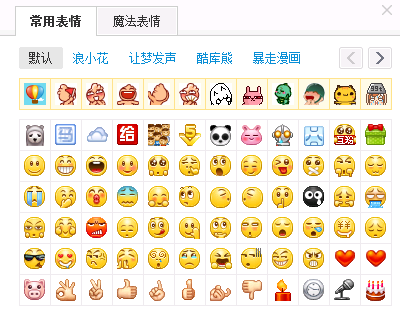
\includegraphics[width=4.1669in,height=3.278in]{figures/chap2/chapitre2-img1.png}
    \caption[Un jeu d{\textquoteright}émoticônes de Weibo]{Un jeu d{\textquoteright}émoticônes sur \url{weibo.com} -- Consulté le 10 Aout 2013 à 10:00 GMT+8}
    \label{fig:emoticons-weibo}
\end{figure}

Il est difficile de définir un mème a priori par la nature de son contenu. Néanmoins, la structure de la diffusion d{\textquoteright}un message peut nous permettre de le décrire comme un mème. Reproduisant en grande partie le cycle de vie classique d{\textquoteright}une information comme une rumeur ou une \textit{news, }les mèmes possèdent des modes de diffusion en ligne assez déterminés et prévisibles. La plupart du temps, ils sont mis en circulation sur un petit nombre de sites spécialisés, avant d{\textquoteright}être repris dans une première phase par un assez petit nombre d{\textquoteright}utilisateurs qui se charge de les publier sur les réseaux sociaux \citep{Bauckhage2011}. Les réseaux sociaux agissent alors comme une chambre d{\textquoteright}écho, qui détermine si le {\textquotedblleft}proto-mème{\textquotedblright} encore en devenir deviendra mème ou restera simple message isolé. Durant cette phase souvent nommée \textit{adoption,} le mème entre en concurrence avec d{\textquoteright}autres informations sur les réseaux sociaux o\`u les utilisateurs sont sans cesse \ sollicités par d{\textquoteright}autres informations \citep{Davenport2001}. Si l{\textquoteright}attention générée par le mème auprès des utilisateurs atteint un pic suffisamment important, il faut environ 2h30 pour que les mèmes rejoignent les pages des médias plus traditionnels en commen\c{c}ant par les blogs, puis les sites d{\textquoteright}information \citep{Leskovec2009}. Ensuite, l{\textquoteright}attention envers le mème décroit fortement et rapidement. La présence épisodique de citations maintient l{\textquoteright}existence du mème apparente dans des groupes définis \citep{Buchel2012}.

\begin{figure}[h]
    \centering
    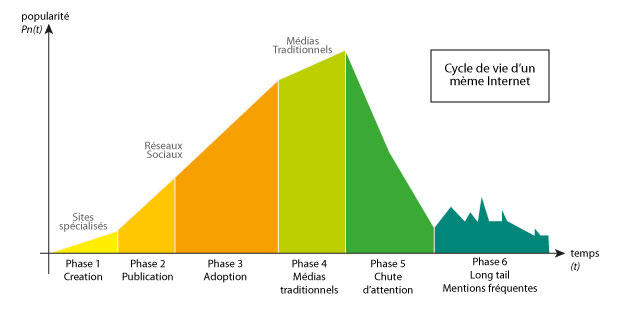
\includegraphics[width=6.2559in,height=3.1559in]{figures/chap2/chapitre2-img2.jpg}
    \caption[Cycle de vie d{\textquoteright}un mème Internet]{Cycle de vie d{\textquoteright}un mème Internet -Clément Renaud - 2013}
    \label{fig:meme-lifecycle}
\end{figure}

L{\textquoteright}évolution du volume de la diffusion permet donc de définir un mème Internet. Néanmoins, il est impossible de donner une estimation du volume minimum pour devenir {\textquotedblleft}mème{\textquotedblright} tant ce chiffre dépend de la population étudiée : il existe des mèmes à très forte diffusion comme le smiley ; d{\textquoteright}autres mèmes se diffusent seulement au sein de groupes d{\textquoteright}individus restreints sans s{\textquoteright}étendre en-dehors. Ainsi, certains mèmes peuvent avoir connu une diffusion très importante dans un groupe, mais rester absolument inconnu du reste de l{\textquoteright}Internet. Une étude de 2012 comparant la diffusion de nombreux mèmes sur Twitter montre que les utilisateurs tendent à choisir les mèmes selon la structure de leur réseau social et le moment d{\textquoteright}exposition, produisant ainsi une grande hétérogénéité des mèmes dans le réseau \citep{Weng2012}. Ainsi, il est hasardeux d{\textquoteright}essayer de décrire le concept de mème par son contenu tant les sujets et les discussions varient. 

Quelques éléments d{\textquoteright}ordre grammaticaux peuvent néanmoins être observés dans la forme que prennent les contenus, appelé parfois {\textquotedblleft}véhicule{\textquotedblright} du mème. Les mèmes qui sont diffusés les plus largement sont composés d{\textquoteright}images et de vidéo. L{\textquoteright}économie d{\textquoteright}attention très limitée de l{\textquoteright}Internet et les modes de lecture sur écran dans un contexte d{\textquoteright}abondance d{\textquoteright}informations font que l{\textquoteright}on privilégie souvent les médias visuels sur le texte \citep{Goldhaber2006}. Un autre élément important est la facilité avec laquelle un message peut être approprié par un utilisateur qui veut le modifier ou tout simplement le diffuser dans le réseau. L{\textquoteright}existence des mèmes est en effet largement conditionnée par la possibilité d{\textquoteright}une diffusion à moindre co\^ut et effort pour l{\textquoteright}utilisateur final, la plupart du temps non-rémunéré. Ici on voit émerger une structure visuelle caractéristique du mème : une image accompagnée d{\textquoteright}une légende écrite en caractères blancs détourés de noir, ou de caractères blancs sur fond noir. L{\textquoteright}utilisation de haut contraste de couleur dans les typographies permet de faire apparaitre très efficacement des légendes juxtaposées à l{\textquoteright}image.

\begin{figure}[h]
    \centering
    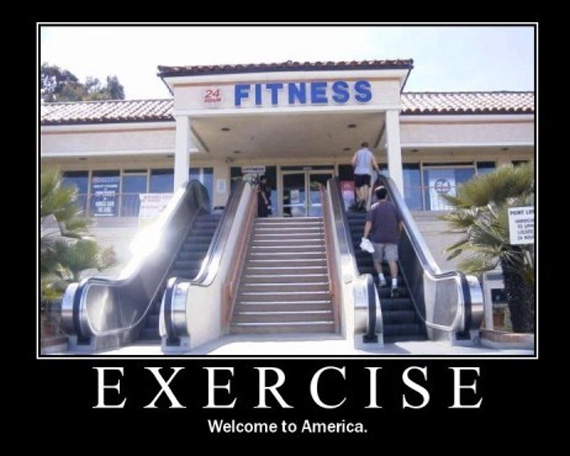
\includegraphics[width=3.6335in,height=2.9114in]{figures/chap2/chapitre2-img3.jpg}
    
\includegraphics[width=2.2559in,height=2.9449in]{figures/chap2/chapitre2-img4.jpg}
    \caption[Exemples de mèmes internet]{Exemples de mèmes Internet, d{\textquoteright}après \url{http://knowyourmeme.org}, consulté le 12/08/2013 à 10 :01 GMT+8}
    \label{fig:memes-examples}
\end{figure}

L{\textquoteright}usage d{\textquoteright}images légendées est une des formes les plus communes pour les mèmes Internet, en particulier ceux de nature comique ou absurde. La mise en place de sites permettant de générer rapidement ce type d{\textquoteright}images légendées (memegenerator.com, mememachine.com, etc.) renforcent l{\textquoteright}unité formelle des mèmes sur l{\textquoteright}Internet, ou plutôt sur l{\textquoteright}Internet anglophone et francophone notamment. En effet, on constate que cette forme typique du mème ne se retrouve pas sur l{\textquoteright}Internet chinois qui utilise plus volontiers des montages d{\textquoteright}images ou des jeux de mots, avec davantage de diversité dans les formes que peuvent prendre les différents mèmes.

\section[Mème, mémoire collective et culture]{Mème, mémoire collective et culture}
\subsection[La mémoire comme trace]{La mémoire comme trace}

Si le concept de mème est souvent considéré comme très récent, on peut néanmoins le resituer dans le vaste paysage des travaux sur la mémoire collective qui ont existé depuis le XIXème siècle \citep{Laurent1999}. Max Stirner dans son livre \textit{The Ego and Its Own }\citeyear{Stirner1995} énonce déjà l{\textquoteright}idée que les individus sont sujets à la circulation de concepts issus de souvenirs communs ou illusoires, comme notamment le nationalisme et la religion. Le logicien Bertrand Russell reprend par la suite dans son livre \textit{The Analysis of Mind } (\citeyear{Russell1921}) les travaux sur la mémoire et l{\textquoteright}évolution sociale du physiologiste allemand \cite{Semon1923}. Utilisant le concept central de \textit{mneme} (du grec 
% μνήμη
\textit{mneme}, mémoire), Semon travaille sur l{\textquoteright}idée de \textit{{\textquotedblleft}traces mnésiques{\textquotedblright} }laissées par les diverses expériences au niveau cellulaire comme au niveau de l{\textquoteright}organisme tout entier. La psychanalyse a également cherché à saisir cette distance impalpable entre expérience et organisme en interrogeant les marques laissées par les souvenirs. Pour Freud comme pour Semon, {\textquotedblleft}l{\textquoteright}appareil psychique{\textquotedblright} de la mémoire se constitue sous la forme de {\textquotedblleft}traces{\textquotedblright}, qu{\textquoteright}il se refuse néanmoins à localiser dans des zones spécifiques du cerveau. Lacan après lui suggèrera que la perception et la mémoire des expériences se structurent dans le langage lui-même, seul outil de connaissance du monde. Depuis les dix dernières années, plusieurs découvertes dans le domaine de la neurologie viennent corroborer cette idée que la mémoire existe sous forme de traces. Les travaux autour de la \textit{plasticité neuronale }montrent notamment l{\textquoteright}existence de la mémoire sous la forme de connections, relations ténues ancrées dans notre réseau neuronal global \citep{Magistretti2008}.  

\begin{table}[htbp]
    \centering
    \begin{tabulary}{\textwidth}{L|C C C}
        
        ~ & t=1  & t=2  & t=3 \\[2ex]
        
        \hline \\ [-1.5ex]
    
        Freud  & expérience  & perception  & Traces mnémiques et psychiques \\[3ex]

        Lacan & expérience (signifié)  &   perception (signifié)  &   Signifiant (traces structurées dans le langage) \\[3ex]

        Neurosciences &  expérience & Perception & Traces synaptiquesassemblages de neurones \\[3ex]

    \end{tabulary}

    \caption{ Etapes constituantes de la mémoire - Convergence entre la trace psychique et synaptique \citep{Ansermet2004} }
\end{table}

Ces disciplines s{\textquoteright}intéressent majoritairement à l{\textquoteright}étude de la constitution d{\textquoteright}une mémoire individuelle, ne nous livrant que peu de clés pour comprendre les éléments qui font qu{\textquoteright}une mémoire devient commune. Le paléontologiste Leroi Gourhan propose dans son livre \textit{L{\textquoteright}homme et la Matière} (\citeyear{Leroi-Gourhan1971}) de considérer que les humains possèdent trois formes de mémoire : une mémoire individuelle sensible, stockée dans les organes du corps ; une mémoire héritée génétiquement, stockée dans l{\textquoteright}ADN ; et une troisième forme de mémoire, transmise de générations en générations : la \textit{technologie}. Dans sa lecture de Leroi-Gourhan, Stiegler (1998b) explique comment \textit{l{\textquoteright}objet technologique} porte en lui les traces des expérimentations, réussites et échecs, mémoire cumulative de temps et de sociétés passées, à la fois héritée et commune, transmissible par son usage.

\begin{table}[htbp]
    \begin{tabulary}{\textwidth}{L|C C}
        \centering
        \textbf{Forme de mémoire} &  \textbf{Contenu}  & \textbf{Stockage} \\[3ex]
        \hline \\ [-1.5ex]
        génétique  &  Particularités héritées des ancêtres   &  DNA \\[3ex]
        
        épigénétique   &  Mémoire sensible de l’expérience personnelle   &  Organes, nerfs, cerveau \\[3ex]
        
        technologique  &  Pratiques de la vie quotidienne en société (usages) & Objets technologiques \\[3ex]
    \end{tabulary}
    \caption{Les trois formes de mémoire d{\textquoteright}après Leroi-Gourhan et Stiegler}
\end{table}


\subsection[Diffusion de mèmes et structuration d{\textquoteright}une mémoire collective]{Diffusion de mèmes et structuration d{\textquoteright}une mémoire collective}
La relation entre mémoire humaine et mémoire technologique est au centre de notre étude. La technologie a depuis toujours été considérée comme une mémoire extérieure. Dans \textit{Phèdre}, Platon raconte l{\textquoteright}histoire du roi égyptien Thamous recevant en cadeau du dieu Thot l{\textquoteright}écriture, le remède (\textit{pharmakon) }qui devait \textit{{\textquotedblleft}soulager la science et la mémoire{\textquotedblright} }(Platon, 274e). Le roi Thamous, effrayé par cette nouvelle technologie de la mémoire écriture se voit saisi de l{\textquoteright}angoisse d{\textquoteright}une perte de cette mémoire. Avec la fin de cette oralité, la disparition de la méthode active des antiques thé\^atres de la mémoire au profit d{\textquoteright}un support inerte et extérieure pourrait-t-elle sceller l{\textquoteright}avènement d{\textquoteright}une nouvelle bêtise? Aujourd{\textquoteright}hui, l{\textquoteright}importance grandissante des bases de données et de connaissances soulèvent encore une fois les mêmes questions, toujours irrésolues. Nicolas Carr constate notamment que \textit{{\textquotedblleft}l{\textquoteright}Internet nous rend stupide{\textquotedblright}} et que son usage répété entraine une baisse drastique de nos facultés de concentration \citep{Carr2010}. A l{\textquoteright}ère du Big Data et de l{\textquoteright}expansion sans fin de notre mémoire numérique, la constitution de nos bases de données interroge notre construction d{\textquoteright}une mémoire collective. Les mèmes Internet, d{\textquoteright}abord gravés dans les disques durs des serveurs, viennent être actualisés par ceux qui les partagent, les commentent, jouent avec et se les approprient. L{\textquoteright}exemple de l{\textquoteright}Internet chinois nous montre la volatilité de cette mémoire numérique, artefact historiographique d{\textquoteright}une culture soumise au bon-vouloir des administrateurs du réseau. Le \textit{Manifeste de l{\textquoteright}Archiviste} publié par \cite{Hui2014} s{\textquoteright}ouvre sur l{\textquoteright}angoissante interrogation deleuzienne :  

\begin{quote}
\textit{
    ``Un nouvel archiviste est nommé dans la ville. Mais est-il à proprement parler nommé ? N'est-ce pas sur ses propres instructions qu'il agit ?''
}
\citep{Deleuze1972a}.
\end{quote}

L{\textquoteright}existence et l{\textquoteright}usage quotidien des bases de données questionnent chaque jour l{\textquoteright}assujettissement des symboles de notre mémoire à l{\textquoteright}objet technologique, à la fois béquille, prothèse et maquillage postiche de notre détestable devenir bête. Les petits \textit{mèmes Internet}, habitant des profondeurs glacées des \textit{data centers}, nous parviennent en dansant, d{\textquoteright}abord sur nos écrans puis dans un coin de notre tête. Avec l{\textquoteright}usage répété des technologies et de l{\textquoteright}écriture numérique, les frontières entre milieu numérique et mémoire collective s{\textquoteright}estompent pour laisser entrevoir un enchevêtrement de silicium, d{\textquoteright}idées et de chair, constitutifs de notre savoir moderne. 

Poursuivant l{\textquoteright}idée d{\textquoteright}une archéologie du présent introduite par Foucault, il s{\textquoteright}agit donc de documenter les processus par lesquels ces obscurs habitants des bases de données viennent laisser leurs traces pour constituer des bribes de nos mémoires collectives. Maurice Halbwachs dans son vaste travail aborde les fa\c{c}ons dont l{\textquoteright}histoire structure l{\textquoteright}être-ensemble des groupes humains. En disant que \textit{"l'histoire de notre vie fait partie de l'histoire en général"}\citep{Halbwachs1947}, il identifie une mémoire autobiographique (personnelle) et une mémoire historique (sociale). Les inquiétudes et considérations autour de la {\textquotedblleft}vie privée{\textquotedblright} sur Internet illustrent les liens intimes entre ces deux mémoires aux frontières devenant aujourd{\textquoteright}hui chaque jour plus poreuses. L{\textquoteright}acte singulier et autobiographique devient sous l{\textquoteright}effet du réseau un fait social, disponible à tout moment dans {\textquotedblleft}l{\textquoteright}historique{\textquotedblright} qui se déroule sous le curseur. L{\textquoteright}oubli devient alors un commerce très prisé permettant de garantir la limite entre la mémoire autobiographique de la fin de soirée de samedi dernier et la mémoire socialement acceptable du CV du chercheur d{\textquoteright}emploi. \'A l{\textquoteright}inverse, les photos du dernier voyage en Papouasie ou la pose avec une star de la télé témoignent fièrement d{\textquoteright}un lien mémoriel entre autobiographie et histoire commune. Les \textit{mèmes} se propagent ainsi d{\textquoteright}individus en groupes pour former peu à peu des éléments de mémoire commune. Objets, chansons, histoires, légendes, icônes... se diffusent autour de la toile par des procédés tenant autant de la copie que de l{\textquoteright}appropriation. 

\begin{figure}[htbp]
    \centering
    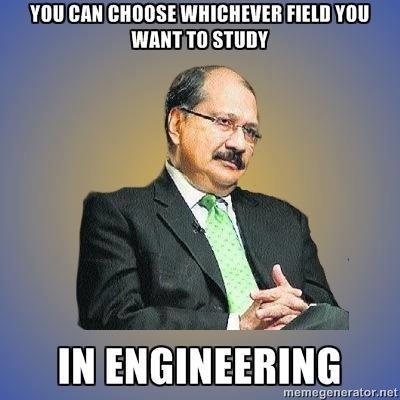
\includegraphics[width=1.6224in,height=1.6224in]{figures/chap2/chapitre2-img5.jpg}
    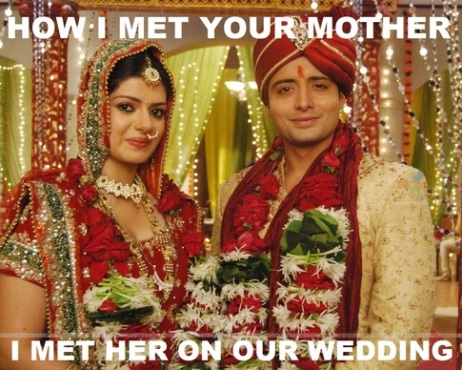
\includegraphics[width=2.0449in,height=1.6335in]{figures/chap2/chapitre2-img6.jpg}
    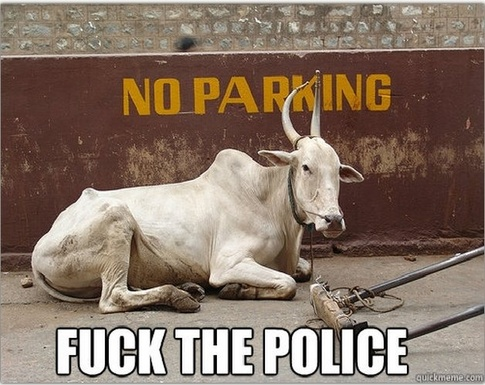
\includegraphics[width=2.078in,height=1.6449in]{figures/chap2/chapitre2-img7.jpg}
    \caption[Réponses à la question à propos des mèmes indiens sur Quora]{Exemples de réponses à la question \textit{"What are some quintessential Indian memes ?"} D'après \url{http://www.quora.com/India/What-are-some-quintessential-Indian-memes}, Consulté le 12/08/2013 à 0 :41 GMT+8 }
    \label{fig:quora-india}
\end{figure}


Le site de questions/réponses \textit{Quora.com} offre un regard intéressant sur la question : \textit{{\guillemotleft}~What are some quintessential Indian memes ?~{\guillemotright}.} Les utilisateurs répondent donc en ajoutant des exemples de mème qui semblent appartenir dans leurs esprits à la {\textquotedblleft}quintessence des mèmes indiens {\textquotedblright}. 
 Avec plusieurs centaines d{\textquoteright}images postées par des
utilisateurs majoritairement indiens, nous pouvons constater plusieurs choses : 

\begin{itemize}
    \item \textbf{Langue}: à part trois réponses, la totalité des réponses sont en anglais. Cela peut s’expliquer par le fait que l’anglais est une langue de communication majoritaire en Inde, et également par le fait que le site Quora.com n’accepte habituellement que des réponses en anglais.
    \item \textbf{Forme}: à l’exception de quatre réponses, les mèmes revêtent tous la forme « classique » : photo retouchée et légendé par un texte en anglais aux lettres blanches sur fond ou détour noir.
    \item \textbf{Humour}: la plupart des réponses sont de nature comique.
    \item \textbf{Récurrence}: certaines images sont très récurrentes et si les légendes diffèrent, le sens reste le même.
    \item \textbf{Thématiques diverses}: de nombreux messages traitent de la vie de famille (parents, mariage), de loisirs (cricket), de la vie quotidienne (achats, école , etc.) et un peu de politique.
\end{itemize}

L{\textquoteright}image la plus citée représente la figure d{\textquoteright}un père autoritaire :

\begin{figure}[htbp]

    \subfloat[\textit{"High Expectations Indian Father"}]{
        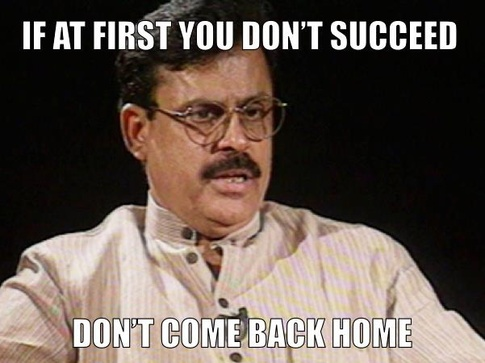
\includegraphics[width=2.0449in,height=1.5in]{figures/chap2/chapitre2-img8.jpg}
        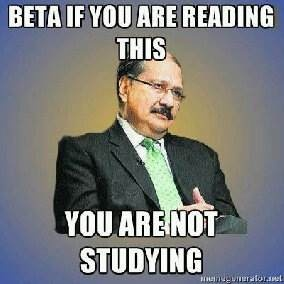
\includegraphics[width=1.5335in,height=1.5in]{figures/chap2/chapitre2-img9.jpg}
        
\includegraphics[width=1.8224in,height=1.5in]{figures/chap2/chapitre2-img10.jpg}
        \label{fig:severe-indian-dad}
    }
    \newline
    \subfloat[\textit{"High Expectations Asian Father"}]{
        \label{fig:severe-chinese-dad}
        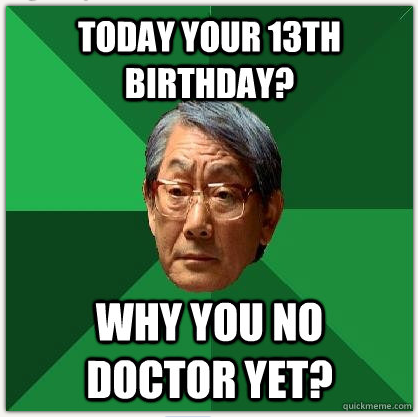
\includegraphics[width=1.9335in,height=1.9in]{figures/chap2/chapitre2-img11.png}
        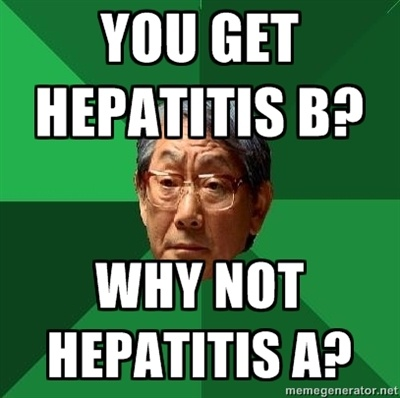
\includegraphics[width=1.9004in,height=1.9in]{figures/chap2/chapitre2-img12.jpg}
        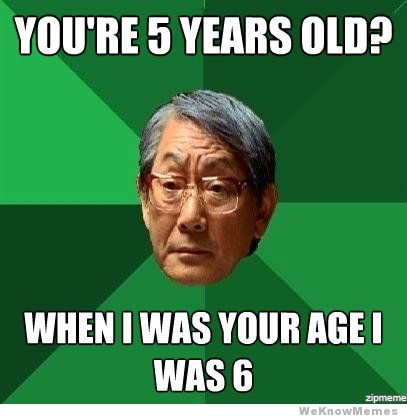
\includegraphics[width=1.8449in,height=1.9in]{figures/chap2/chapitre2-img13.jpg}
    }
    \caption[Mème ``High Expectations Asian Father'' d'après Quora.com]{Exemples du mème \textit{"High Expectations Asian Father"} D{\textquoteright}après {\textquotedblleft}\textit{What are the funniest High Expectations Asian Father meme images?{\textquotedblright}} sur Quora.com \url{http://www.quora.com/Memes/What-are-the-funniest-High-Expectations-Asian-Father-meme-images}, Consulté le 12/08/2013 à 10:56}
\end{figure}

La définition des mèmes faites par Blackmore ne correspond pas nécessairement à ce que nous observons ici. L{\textquoteright}unité formelle de l{\textquoteright}ensemble de ces mèmes (image avec des caractères blancs cerclés de noirs) propose une définition bien plus restreinte. Néanmoins, nous pouvons comprendre qu{\textquoteright}il s{\textquoteright}agit bien de la manifestation d{\textquoteright}une culture particulière. L{\textquoteright}image d{\textquoteright}une vache assise devant un sigle \textit{{\textquotedblleft}Fuck The Police{\textquotedblright} }serait en effet un absolu non-sens sans la référence à l{\textquoteright}Inde o\`u les vaches sont sacrées et jouissent de droits particuliers que même la police ne peut entraver. Ainsi, il existe bel et bien des pré-requis pour comprendre ou actualiser un mème. Les plus évidents sont :

\begin{itemize}
    \item \textbf{L’accès et l’usage de la bonne technologie}: Il est nécessaire pour un utilisateur de posséder et de savoir utiliser la technologie par laquelle le mème est diffusé.
    \item \textbf{La langue}: Le message possède une légende donc l’utilisateur doit pouvoir la lire et la comprendre.
    \item \textbf{Les implicites} : L’utilisateur doit posséder le socle de références communes et d’implicites qui sont impératifs pour pouvoir comprendre le message. 
\end{itemize}

Nous observons ici de très larges et vagues groupes ({\guillemotleft}~\textit{indiens}~{\guillemotright}, {\guillemotleft}~\textit{asiatiques}~{\guillemotright}{\dots}) sans pouvoir vraiment comprendre dans le détail ce qui peut réellement constituer des éléments communs. Les travaux sur la formation des {\textquotedblleft}communautés{\textquotedblright} en ligne ont montré comment la circulation des objets digitaux peut posséder une fonction de catharsis pour des groupes plus réduits \citep{Steyer2006}. Néanmoins, on voit bien qu{\textquoteright}ici l{\textquoteright}appartenance pré-existe puisque le mème nécessite de nombreux pré-requis pour le comprendre. Le langage et son expressivité par l{\textquoteright}humour sont notamment des contraintes incompressibles pour l{\textquoteright}actualisation de ce mème par un individu. Néanmoins nous pouvons voir dans ce cas particulier que le mème participe à l{\textquoteright}affirmation de l{\textquoteright}existence du groupe, avec la figure redondante de caractéristiques communes du père, affirmant par la dérision une forme de paternité commune aux membres de ce groupe. D{\textquoteright}autres mèmes ne nécessitent pas tant de références, ce qui contribue largement à leurs diffusions. La vidéo du clip musical \textit{Gangnam Style} du chanteur Psy a notamment atteint des records inégalés en termes de diffusion\footnote{ Première vidéo à avoir officiellement dépassée le milliard de vues sur Youtube. 1,733,769,243 vues, consulté le 13/08/2013 à 09 :35 GMT+8 \url{http://www.youtube.com/watch?v=9bZkp7q19f0}} gr\^ace à une très vaste campagne télévisuelle et sur internet. La diminution des implicites et la standardisation de l{\textquoteright}écriture utilisée a sans doute contribué la diffusion, avec un langage du corps quasi universel, le pas de danse. Formellement, il s{\textquoteright}agit d{\textquoteright}un vidéo clip très classique dont la structure et le montage sont largement familiers du public. Les attributs des personnages du clip sont également de grands classiques du vidéo clip commercial : voitures, belles filles et bijoux en or. La présence d{\textquoteright}un quartier spécifique de Séoul en Corée du Sud agit ici comme un attribut du contenu mais aucune des références ne nécessite de préalable linguistique particulier. De plus, les mystères de la musique et de la scénographie agissent bien évidemment au-delà de toute analyse formelle pour faire de ce hit un des mèmes Internet les plus connus dans le monde. 
Les méméticiens disposent classiquement de deux procédes pour
analyser la diffusion des mèmes: 

\begin{itemize}
\item
\textbf{La contamination~\newline
}Le mème se déplace à la manière d{\textquoteright}un virus, en contaminant les sujets les plus susceptibles de l{\textquoteright}être lors d{\textquoteright}une phase d{\textquoteright}exposition. L{\textquoteright}exemple le plus classique pour ce modèle est la diffusion des croyances religieuses
qui agirait par contagion \citep{Dennett2006}
\item
\textbf{La réplication~\newline
L}es activités culturelles humaines procèdent de l{\textquoteright}imitation, notamment au travers de phases cruciales d{\textquoteright}apprentissage. Ainsi, les mèmes existent et se diffusent dans toutes activités nécessitant une imitation : \textit{{\textquotedblleft}} \textit{If we define memes as transmitted by imitation then whatever is passed on by this copying process is a meme.{\textquotedblright} }\citep{Blackmore2006}. 
\end{itemize}

Le modèle épidémique de diffusion vient appuyer la vision éthologique du mème. Adaptée de la virologie, les {\guillemotleft}~sujets à risque~{\guillemotright} seraient plus à même d{\textquoteright}être {\guillemotleft}~contaminés~{\guillemotright} par une {\guillemotleft}~exposition~{\guillemotright} suffisamment longue à tel ou tel mème \citep{Wang2011}. Blackmore définit néanmoins trois phases indispensables pour reconna\^itre un mème comme tel:  

\begin{quote}
\textit{``Memes fulfill the role of replicator because they exhibit all three of the necessary conditions; that is, \textit{heredity} (the form and details of the behavior are copied), \textit{variation} (they are copied with errors, embellishments or other variations), and \textit{selection} (only some behaviors are successfully copied).''}, d'après \cite{Blackmore2006}
\end{quote}

Les trois aspects sont indissociables et forment selon Blackmore un {\textquotedblleft}\textit{véritable processus évolutioniste{\textquotedblright} }\citep{Blackmore2006}. La définition quasi tautologique du mème ({\guillemotleft}~\textit{Whatever is passed on{\guillemotright}}) montre bien comment le mème en tant que concept est considéré chez Blackmore non pas comme un phénomène mais plutôt comme un objet en-soi. La définition du mème en tant qu{\textquoteright}objet autonome se heurte dès l{\textquoteright}abord au risque de devenir un pur artefact de l{\textquoteright}observation, n{\textquoteright}existant que dans l{\textquoteright}esprit de l{\textquoteright}observant. Alors que Dawkins met en garde non sans humour que son livre \textit{The Selfish Gene} \textit{{\textquotedblleft}devrait être lu presque comme s{\textquoteright}il était de la science-fiction{\textquotedblright} }\citep{Dawkins1989}, la faiblesse des modèles de diffusion des mèmes vu comme un réplicateur ou comme un virus ne recouvre que partiellement la réalité observée empiriquement pour les mèmes Internet. Ainsi, l{\textquoteright}appartenance des individus à tel ou tel groupe pré-existe au mème. Dans son appropriation se joue davantage l{\textquoteright}expression d{\textquoteright}un sentiment d{\textquoteright}appartenance qu{\textquoteright}une contamination qui nierait les termes de sa volonté individuelle pour y substituer l{\textquoteright}individu comme sujet du mème.  


\section[Textualité des mèmes et formes d{\textquoteright}énonciations numériques]{Textualité des mèmes et formes d{\textquoteright}énonciations numériques}

\subsection[Le mème comme figure rhétorique de l{\textquoteright}écriture intertextuelle]{Le mème comme figure rhétorique de l{\textquoteright}écriture intertextuelle}

 
Le mème peut être défini comme une série d{\textquoteright}actes \textit{d{\textquoteright}énonciation} qui contribuent à l{\textquoteright}existence et la reconnaissance mutuelles d{\textquoteright}individus comme groupe. Cette définition s{\textquoteright}oppose à l'idée d{\textquoteright}une entité de sémantique autonome qui serait constitutif d{\textquoteright}une hypothétique culture commune. Les partages, commentaires, réappropriations puis transformations des \textit{mèmes Internet }nous serviront de supports pour comprendre les \textit{actes d{\textquoteright}énonciation. }Ces courts messages faits de texte, image ou vidéo sont en quelque sorte les voix, répétitions, annonances et redites d{\textquoteright}une foule d{\textquoteright}individus et de groupes qui habitent la Toile. Au-delà de l{\textquoteright}idée d{\textquoteright}un {\textquotedblleft}objet{\textquotedblright} numérique qui réifierait les actions en une substance figée, nous nommons \textit{énonciation} le moment d{\textquoteright}existence observable o\`u se manifeste un mème. Comme pour les émoticones, les pratiques actuelles de l{\textquoteright}écriture en ligne des mèmes Internet sont à envisager comme des formes renouvelées d{\textquoteright}oralité. Email, chat ou réseaux sociaux, ces discussions font partie d{\textquoteright}une \textit{{\textquotedblleft}oralité seconde{\textquotedblright} }\citep{Ong1988} constituante des technologies de l{\textquoteright}écrit à l{\textquoteright}ère du numérique. Contrairement à l{\textquoteright}oralité première des illettrés, cette oralité seconde est structurée par l{\textquoteright}usage des technologies et notamment les structures formelles de l{\textquoteright}écriture pour le média :  

\begin{quote}
    \textit{``Telephone, radio, television and the various kind of sound tape, electronic technology has brought us into the age of {\textquoteleft}secondary orality{\textquoteright}. This new orality has striking resemblance to the old in its participatory mystique, its fostering of a communal sense, its concentration on the present moment, and even its use of formulas. But it is essentially a more deliberate and self-conscious orality, based permanently on the use of writing and print, which are essential for the manufacture and operation of the equipment and for it use as well.''} 
\citep{Ong1988}
\end{quote}

L{\textquoteright}hypothèse de Ong est ici que l{\textquoteright}oralité des écritures numériques est une forme manufacturée de l{\textquoteright}expression orale, à laquelle préside la production (industrielle) des technologies. Les services de réseaux sociaux en ligne confirment l{\textquoteright}hypothèse première de Ong puisque \textit{Sina Weibo }ou \textit{Twitter} contraint industriellement l{\textquoteright}écriture à une longueur maximum de 140 caractères. Néanmoins, l{\textquoteright}oralité du mème Internet et plus généralement des écritures numériques ne procède pas seulement de cette écriture conditionnée mais également de la mise en relation des textes : l{\textquoteright}intertextualité. Là o\`u pour Ong l{\textquoteright}industrie médiatique vient contraindre l{\textquoteright}écriture pour la réifier en produit industriel simulant l{\textquoteright}oral, l{\textquoteright}intertextualité vient subvertir ces limites imposées en renvoyant le lecteur à la page suivante.  

En effet, le langage des nouveaux médias ne se contente pas de proposer des nouvelles opérations d{\textquoteright}interactions et de navigations mais s{\textquoteright}inscrit également dans de nouveaux modes de lecture et de narration \citep{Manovich2001}. Une des grandes difficultés pour l{\textquoteright}analyse textuelle et narrative dans le cadre des nouveaux médias est de comprendre o\`u commence et o\`u se termine le texte. La structure éminemment relationnelle du discours narratif en ligne et son intertextualité en font un objet mal défini, que ses auteurs n{\textquoteright}ont pas signé d{\textquoteright}un point final. L{\textquoteright}étude des discursivités hypertextuelles s{\textquoteright}apparenterait donc davantage à l{\textquoteright}étude des formes dans les contes et légendes qu{\textquoteright}aux études herméneutiques classiques sur des textes finis \citep{Clement1995}. Comme le note Lévi-Strauss dans son travail sur Propp, même si les contes possèdent souvent une structure similaire, leur étude en tant qu{\textquoteright}élément culturel n{\textquoteright}est révélatrice que dans un contexte précis et incarné. Il est inutile de vouloir extraire une supposée intention culturelle du texte car on se doit de le comprendre lors de son énonciation, sur la place d{\textquoteright}un marché au Maroc avec les conteurs de Ben Jelloun ou au pied du lit d{\textquoteright}un jeune Européen avec les histoires compilées par les frères Grimm. Héritant à la fois des pratiques culturelles et folkloriques anciennes tout en se renouvelant sous les nouvelles contraintes de la technologie \citep{Barber2008}, le mème est lui aussi à comprendre dans son contexte d{\textquoteright}énonciation. De récents travaux travaillent à comparer les modes de diffusion des mèmes avec ceux des traditions folkloriques \citep{Seta2014}. En considérant les mèmes Internet comme un {\textquotedblleft}\textit{folklore numérique}{\textquotedblright}, on comprend mieux la nature presque auto-référentielle de la relation entre le mème et la culture qui le voit na\^itre. La transmission d{\textquoteright}éléments particuliers dans la discursivité du mème en fait une figure rhétorique d{\textquoteright}énonciation de sa propre origine. 

Le large pouvoir fédérateur de certains mèmes fascine. Diffusés très largement, \ on se plait à imaginer comment ils peuvent réunir en leur sein des groupes et individus distants, auparavant inconnus et étrangers. L{\textquoteright}importance croissante d{\textquoteright}Internet dans l{\textquoteright}émergence de groupes d{\textquoteright}intérêts et d{\textquoteright}activités voit les études sur la formation de communautés en ligne fleurir. Néanmoins, il nous semble important de se questionner sur la nature des relations créée lors des discussions partagées en ligne. Est-ce bien là le fait d{\textquoteright}une réelle rencontre comme le croient les plus enthousiastes? Ou au contraire est-ce le produit d{\textquoteright}une machine médiatique et décérébrante qui produit du lien sans engendrer de rencontres comme le pensent les plus pessimistes? Cette vaste question est sans doute un des enjeux centraux des questionnements autour de l{\textquoteright}Internet, notamment pour le management et les sciences de gestion. Si l{\textquoteright}énonciation est une pratique structurante pour un individu ({\textquotedblleft}je suis{\textquotedblright}), elle peut l{\textquoteright}être également pour un groupe ({\textquotedblleft}nous sommes{\textquotedblright}). Dans la perspective empirique o\`u nous nous situons, il nous faut tout d{\textquoteright}abord interroger les pratiques du langage pour mieux comprendre comment les discursivités d{\textquoteright}un mème peuvent agir sur les groupes. Le mème considéré comme un acte d{\textquoteright}énonciation se caractérise non seulement par sa manifestation langagière, mais également par l{\textquoteright}intention qu{\textquoteright}il contient. Dans le cadre des réseaux sociaux, nous ne disposons que de très peu d{\textquoteright}éléments sur l{\textquoteright}intention car les données disponibles sur les réseaux sociaux sont par définition le résultat d{\textquoteright}actions passés (écriture, clics, etc.).\textit{ }Nous devons donc développer un modèle à la fois conceptuel et pratique pour nous permettre d{\textquoteright}étudier ces phénomènes d{\textquoteright}énonciation dans le cas particulier des mèmes Internet. Wittgenstein dans ses \textit{Recherches Philosophiques }défend une analyse pragmatique du langage en écrivant : \textit{{\textquotedblleft}Don{\textquoteright}t ask for the meaning, ask for the use.{\textquotedblright}} \citep{Wittgenstein2004}. Il s{\textquoteright}agit de comprendre les jeux langagiers non pas comme un champ linguistique mais comme un ensemble d{\textquoteright}actes qui font sens en contexte et possèdent une intention. 

\begin{quote}
{\textquotedblleft}
\textit{Expressions have meanings even when they are not being used, but it is only in using expressions that a person means something.}
{\textquotedblright} \citep{Bach1994}
\end{quote}

Austin dans ses lectures sur William James met au centre du langage sa dimension pragmatique et propose de comprendre comment on \textit{{\guillemotleft}~fait des choses avec les mots~{\guillemotright}} \citep{Austin1975}. Ses le\c{c}ons présentent une manière nouvelle de catégoriser les différents actes d{\textquoteright}énonciation et montrent la grande diversité des éléments non-linguistique présents dans ces actes. Austin introduit le concept de \textit{performativité }pour nommer le processus qui permet de construire par le langage une réalité extérieure au langage. Les mots ne nomment pas seulement les choses mais peuvent également les faire changer, voire les fabriquer. Austin s{\textquoteright}intéresse donc aux énoncés selon leurs \textit{sens}, leurs intentions (la \textit{force}) ou leurs \textit{effets}. Le concept de \textit{performativité }a depuis continué son chemin tant en linguistique qu{\textquoteright}en sciences sociales, et plus récemment dans des champs aussi divers que le management ou l{\textquoteright}étude du discours scientifique et des pratiques légales \citep{Denis2006}. Les économistes également ont beaucoup discuté de la performativité des discours économiques sur l{\textquoteright}économie réelle \citep{Mackenzie2006}. Les \textit{cultural studies,} et plus précisément les \textit{gender studies }ont aussi fait un large usage de ce concept pour exprimer l{\textquoteright}influence de la matérialité des mots sur les comportements humains \citep{Butler1993}.  

\begin{quote}
    {\guillemotleft}~\textit{Pour qu{\textquoteright}ils deviennent de {\guillemotleft} véritables {\guillemotright} performatifs, les faits, les théories ou les formules doivent circuler dans des cha\^ines de traduction qui consolident l{\textquoteright}assemblage des entités qui le composent et leur permet d{\textquoteright}acquérir le statut de {\guillemotleft} matters of fact {\guillemotright} ({\dots}). C{\textquoteright}est lorsqu{\textquoteright}ils arrivent à durer, c{\textquoteright}est-à-dire à s{\textquoteright}inscrire dans le monde (par l{\textquoteright}intermédiaire d{\textquoteright}objets, de textes, de dispositifs techniques complexes) que leur performativité s{\textquoteright}accomplit.}~{\guillemotright} \citep{Denis2006}
\end{quote}

Les actes d{\textquoteright}énonciation répétés modèlent donc le corps des personnes et de la société, y \textit{laissant }durablement leurs marques. Les énoncés actualisent les discours des groupes sociaux sur eux-mêmes \citep{Butler1993} et ce caractère performatif est constitutif de l{\textquoteright}énonciation. Les énoncés collectifs que sont les mèmes Internet possèdent également cette dimension performative qui actualise le discours de certains groupes en réalités tangibles. La circulation et la structuration de ces mèmes vient structurer le milieu numérique et peut ainsi influer sur la définition de groupes sociaux et des rapports qu{\textquoteright}ils entretiennent. \'Enoncer à son tour une image ou un mot semble un préalable permettant de dénouer l{\textquoteright}implicite de l{\textquoteright}énoncé et d'accroître la proximité dans l{\textquoteright}expérience. Blackmore évoque en termes évolutionnistes le {\textquotedblleft}potentiel transformatif{\textquotedblright} du mème, avec ce qu{\textquoteright}elle nomme la \textit{variation} puis la \textit{sélection}. Ici ce sont les actes d{\textquoteright}\textit{énonciation} qui forment une praxis du mème. Pour nous, le mème n{\textquoteright}est pas un méta-symbole en évolution mais un réseau de praxis culturelles constitué de multiples d{\textquoteright}actes d{\textquoteright}énonciation. Ainsi, le mème ne peut être simplement {\guillemotleft}~copiée~{\guillemotright} mais a besoin d{\textquoteright}être acté pour exister. Dans la définition du mème de Blackmore comme dans le cas des réseaux sociaux, nous observons que l{\textquoteright}énonciation d{\textquoteright}un mème procède d{\textquoteright}une variation parfois nulle, parfois minimale, parfois importante de sa forme d{\textquoteright}origine. Cette déformation due à l{\textquoteright}énonciation est le propre de la fonction d{\textquoteright}apprentissage, notamment langagier. Le caractère performatif du mème devient visible dans l{\textquoteright}usage approprié de la variation qui en est fait. 

Le succès de l{\textquoteright}intention de l{\textquoteright}énoncé est visible dans son imitation, avec comme garantie l{\textquoteright}erreur ou la variation. Platon dans \textit{La République} puis par la suite Aristote dans sa \textit{Poétique,} s{\textquoteright}interroge sur la notion de \textit{mimesis} définie comme les formes d{\textquoteright}imitation qui permettent soit de reproduire, soit de styliser la nature. Pour Aristote, le but singulier de la mimesis est de mettre à jour la dimension empathique cachée de la nature, de la styliser pour y révéler le continuum de l{\textquoteright}expérience propre à tous les êtres. Plus l{\textquoteright}artiste s{\textquoteright}approche de la nature en se dirigeant vers une imitation {\guillemotleft}~véritable{\guillemotright}, plus il s{\textquoteright}éloigne de la réalité de la nature. L{\textquoteright}importance d{\textquoteright}une approche rhétorique comme par exemple la stylisation devient le véritable moyen d{\textquoteright}accès à la signification profonde des choses. Freud réutilisera le concept de \textit{mimesis} pour décrire l{\textquoteright}énonciation du sens d{\textquoteright}un évènement traumatique passé dans la vie d{\textquoteright}un individu au travers d{\textquoteright}activités créatives (art, parole, rêves etc.). Dans la continuité d{\textquoteright}Aristote, Freud comprend le rêve comme une \textit{mimesis} du passé et du réel, révélant au sujet un objet symbolique enfoui. Peut-être est-il possible de considérer le mème Internet comme une mimesis des groupes sociaux et médiatiques qui le produisent. Les processus de symbolisation et de stylisation jouent en effet un rôle déterminant dans sa diffusion. Acte d{\textquoteright}énonciation, le mème agit alors comme une \textit{mimesis} des activités et états d{\textquoteright}\^ame de groupes d{\textquoteright}individus qui l{\textquoteright}énoncent. S{\textquoteright}il est possible de le revivre plusieurs fois, il prendra peut-être à chaque fois un sens différents. Comme le rêve freudien qui est une manifestation biologique de la mémoire inconsciente se produisant durant le sommeil, le mème se manifeste sous des formes visibles symboliques incarnées, \textit{mimesis} particulière du groupe des individus qui l{\textquoteright}énoncent. 


\subsection[Typologie des mèmes Internet]{Typologie des mèmes Internet}

Habituellement définie comme \textit{{\guillemotleft}~une forme typique de relation non linguistique entre des éléments discursifs.~{\guillemotright}}\footnote{ \textit{Les figures de rhétorique}, Laurent Jenny, Université de Genève, 2003}\textit{, }la figure rhétorique se produit dans l{\textquoteright}intertextualité des redites et commentaires qui réaffirme dans le mème l{\textquoteright}existence d{\textquoteright}un groupe qui le constitue.  

En nous appuyant sur la littérature concernant les figures
rhétoriques, nous pourrions chercher à définir plus
précisément une typologie des mèmes fondée sur les formes du
discours. En grec ancien, le topo\"i défini à la fois un lieu ou un
endroit mais également un ensemble de formes rhétoriques utilisant
des motifs particuliers lors de l{\textquoteright}argumentaire afin de
persuader lors de joutes oratoires. En littérature comme en
mathématiques, le terme de \textit{topos }définit également un
ensemble de catégories ouvertes mais connues,
\textit{{\textquotedblleft}un protocole de description des univers
possibles{\textquotedblright} }\citep{Badiou2006}. Le mème peut donc
être compris comme un \textit{lieu commun, }idée
{\textquotedblleft}re\c{c}ue{\textquotedblright} utilisant des
situations ou des images communes et stéréotypées pour opèrer
une transformation sémantique en jouant sur la répétition
d'éléments (les sèmes du discours). En
rhétorique, l{\textquoteright}usage du topos a pour objectif de
contribuer à la persuasion de l{\textquoteright}auditeur par la
mobilisation subtile d{\textquoteright}éléments de culture commune.
Tout l{\textquoteright}art du rhéteur consiste à trouver un moyen
subtile d{\textquoteright}actualiser un lieu commun en une situation
unique propre au contexte pour convaincre. Dans le discours, il prend
bien souvent la forme de l{\textquoteright}anecdote que la rumeur se
charge de diffuser, sa diffusion étant d{\textquoteright}autant plus
efficace qu{\textquoteright}il possède un caractère amusant ou
railleur \citep{Flaubert1997} Concevoir le mème comme une forme de
pratique rhétorique semblable au lieu commun nous permet de resituer
le phénomène des mèmes Internet dans la continuité historique
des pratiques de l{\textquoteright}écriture et de
l{\textquoteright}énonciation rhétorique, ainsi que de ses
modèles d{\textquoteright}analyse socio-textuelle et littéraire
\citep{Plantin1993}. Ainsi, nous pouvons aborder la lecture des mèmes
Internet sous le jour de leur existence aussi bien formelle (textuelle)
que rhétorique (comme actes d{\textquoteright}énonciations et de
persuasion). Les mèmes tout comme les lieux communs se donnent à
voir d{\textquoteright}abord sous la forme de paradoxes, qui
deviendront eux-mêmes des lieux communs.
L{\textquoteright}originalité d{\textquoteright}un lieu commun en
devenir se définit dans une tension constante entre imitation et
nouveauté, subversion et actualisation de formes canoniques :
\textit{{\textquotedblleft}dialogue de l'horizon
d'attente et de l'écart esthétique, c'est-à-dire le jeu du classique et du moderne, la tension entre le même et l'autre qui existe, dans tout texte et dans toute lecture, entre le plaisir et la jouissance, pour reprendre les mots de Barthes}. \citep{Compagnon1997}

L{\textquoteright}approche des mèmes renouvelée par la nature intertextuelle du langage multimédia montre des caractéristiques  d{\textquoteright}après une centaine de mèmes parmi les plus largement diffusés d{\textquoteright}Internet \citep{Bauckhage2011} :

\begin{enumerate}
\item {\color{black}
\textbf{Humour~}: Le mème doit posséder une dimension comique et
accrocheuse}
\item {\color{black}
\textbf{Intertextualité} : Le mème met en jeu un ou des renvois à
d{\textquoteright}autres éléments culturels ou textuels, souvent
implicites.}
\item {\color{black}
\textbf{Juxtaposition atypique} : Les éléments visuels ou
sémantiques mis en jeu dans le mème ne possèdent pas de
corrélations apparentes et c{\textquoteright}est la mise en relation
de plusieurs objets improbables qui en fait un objet intéressant.}
\end{enumerate}
L{\textquoteright}étude en question nous offre un début de
critères mais porte seulement sur un type précis de mèmes à
caractère plutôt comique, ignorant les discussions plus
sérieuses, d{\textquoteright}ordre politique notamment. La forme
particulière de juxtaposition atypique observée par les auteurs
serait en rhétorique une {\textquotedblleft}\textit{métaphore in
praesentia{\textquotedblright} }décrite comme une
\textit{{\guillemotleft}~figure de rapprochement analogique entre deux
représentations co-présentes~{\guillemotright}} \citep{Jenny2012}. Nous
nous trouvons donc en présence d{\textquoteright}une forme
particulière de mème seulement. Si l{\textquoteright}humour sous
toutes ces formes (blague, sarcasme, ironie, etc.) est un élément
très répandu qui favorise la circulation des contenus en ligne, il
nous semble néanmoins un peu réducteur de se limiter à cette
définition. De nombreux mèmes Internet existent non pas gr\^ace à
l{\textquoteright}humour mais gr\^ace au \textit{pathos}
qu{\textquoteright}ils dégagent. Le mème \textit{Kony2012, }un des
plus diffusés de l{\textquoteright}histoire
d{\textquoteright}Internet, présentait le militaire Ugandais Joseph
Kony dans une vidéo faite d{\textquoteright}images de guerre et
d{\textquoteright}enfants en pleurs\footnote{ \textit{KONY2012: See How Invisible Networks Helped a Campaign Capture the World's Attention}, \textit{Social Flow}, \url{http://alturl.com/zniry} consulté le 28 Février 2014 GMT+1}.
Ainsi, on peut dire que les mèmes Internet utilisent les formes
classiques de la rhétorique adaptées au langage médiatique moderne, 
teinté d{\textquoteright}humour ou de sensationnalisme. En se
saisissant du monde social et politique, les mèmes Internet
produisent d{\textquoteright}intéressants discours sur les faits
qu{\textquoteright}ils relatent - et sur la technologie qui les
produit. Alors que les révolutions du Printemps Arabe avaient
notamment soulevé l{\textquoteright}espoir d{\textquoteright}un monde
meilleur par l{\textquoteright}usage des réseaux sociaux pour
instaurer la démocratie \citep{Lotan2011}, la communication
instantanée via ces mêmes réseaux sociaux devenait quelques
semaines plus tard une des causes majeures de la flambée de violence
durant une série d{\textquoteright}émeutes à Londres \citep{Casilli2011}. Les différentes intentions des discursivités et
actes d{\textquoteright}énonciation à l{\textquoteright}{\oe}uvre
dans un mème peuvent donc nous aider à dresser une typologie des
mèmes. Une typologie des mèmes ne peut être considérée comme
exclusive et les glissements sémantiques et symboliques qui peuvent
s{\textquoteright}opérer nous obligent à considérer une
catégorisation non-exclusive. En nous appuyant sur différents
exemples et sur la littérature, nous dressons une première
ébauche de typologie des mèmes Internet qui sera ensuite
approfondie par l{\textquoteright}étude empirique des données le
c{\oe}ur de notre étude. Pour les exemples, nous essaierons de donner
les références et implicites indispensables permettant de
comprendre le mème dans son intertextualité.

\begin{table}[htbp]
    \centering
    \begin{tabulary}{\textwidth}{ R | C}
    \textbf{Objectifs du mème}  & \textbf{Exemples célèbres et références} \\[1ex]
    \hline \\ [-1.5ex]
    Absurdiste, humour &  LOLCats, Tumblr \citep{Bauckhage2011} \\[1ex]
    \hline \\ [-1.5ex]
    Actualité, satire, commentaire social  & CaoNiMa \citep{Mina2012}, Cute Cat Theory \citep{Zuckerman2008} \\[1ex]
    \hline \\ [-1.5ex]
    Publicité, marketing viral & Gangnam Style \citep{Bolsover2013}, Memetic Marketing \citep{Flor2000} \\[1ex]
    \hline \\ [-1.5ex]
    Marketing politique, soutien, pétition & Obama Ohio Campaign \citep{Walker2012}, Pétitions en ligne (Adamic al.,2013) \\[1ex]
    \hline \\ [-1.5ex]
    Fan clubs, adoration  &  Fan-fiction , Machinima, etc. \\[1ex]
    \hline \\ [-1.5ex]
    Hoax, spam & Email spam, « Nigerian scam » \\[1ex]
    \end{tabulary}

\caption[Typologie des mèmes]{Les différents type de mèmes Internet observables - tableau réalisé d{\textquoteright}après la littérature indiquée}
\label{fig:typologie-memes}

\end{table}


Cette typologie nous permet de poser un premier regard sur des catégories non-exclusives constituant le paysage des mèmes Internet, inspirés d{\textquoteright}exemples et de la littérature existante. Nous pouvons d{\textquoteright}ores et déjà noter que l{\textquoteright}ensemble de ces différentes pratiques pré-existent à l{\textquoteright}Internet et sont souvent la reconduction sous une forme numérique de discursivités pré-existantes (penser à la publicité, la propagande politique ou même les rumeurs). La forme et l{\textquoteright}échelle de la diffusion sont néanmoins des différences importantes ainsi bien s\^ur que \ les situations d{\textquoteright}énonciation (dans une file d{\textquoteright}attente ou devant son ordinateur).

\begin{description}

\item[Absurdiste, humour]
\hfill \\
De nombreux mèmes Internet parmi ceux que nous avons présentés dans la première partie de ce chapitre viennent se classer dans cette catégorie. Connaissant parfois des succès planétaire, un des exemples les plus caractéristiques est celui des {\textquotedblleft}LOLcats{\textquotedblright}, ces vidéos ou images de chats illustrés de citations et autres accessoires comiques. Omniprésent sur la Toile, l{\textquoteright}immense répertoire de photos et de vidéos comiques de chats dans différentes situations (jouant du piano, sautant dans des bo\^ites en cartons, etc.) constitue un des plus visionnés de l{\textquoteright}Internet \citep{Bauckhage2011}.

\begin{figure}[htpb]
    \centering
    
    \subfloat[a LOLcat]{
        
\includegraphics[scale=.72]{figures/lolcats/cat7.jpg}
    }
    \subfloat[another LOLcat]{ 
        
\includegraphics[scale=.15]{figures/lolcats/lolcat_00294386.jpg}
    }
    \caption[Some LOLcats]{Some LOLcats, d{\textquoteright}après le \url{http://www.lolcats.com}, consulté le 4 Avril 2013 à 15:32}
    \label{fig:caonima}
\end{figure}



\item[Actualité, satire, commentaire social]
\hfill \\
En regroupant ces trois catégories, nous souhaitons considérer la pratique ancienne des discussions politiques ou polémiques autour de faits divers ou d{\textquoteright}actualités que l{\textquoteright}Internet vient aujourd{\textquoteright}hui renouveler dans la forme. Nous avons vu précédemment avec les {\textquotedblleft}crabes de rivières{\textquotedblright} (voir \ref{fig:hexie}) comment la satire politique en Chine se manifestait bien souvent sous la forme de mèmes Internet. Par les voies de l{\textquoteright}Internet,de nombreux faits divers sont devenus en Chine des affaires d{\textquoteright}état, influen\c{c}ant le jeu politique et offrant un nouveau canal de diffusion pour les pratique subversives. Connu pour son {\oe}uvre artistique, l{\textquoteright}artiste chinois Ai Weiwei est une des figures célèbres de l{\textquoteright}Internet chinois. Utilisant abondamment blog et microblog, son travail artistique depuis plusieurs années a pris la tournure d{\textquoteright}un bras de fer médiatique avec le gouvernement sur les grandes questions sociétales de la Chine d{\textquoteright}aujourd{\textquoteright}hui. Son père, poète célèbre du régime communiste sous Mao fut déchu durant la révolution Culturelle, transmettant à son fils à la fois un go\^ut pour les arts et une violente amertume pour le pouvoir en place à Pékin. Critiquant ouvertement la corruption des officiels et de la police, Ai Weiwei a vu régulièrement ses comptes Internet de blog et microblog fermés, notamment par le service Sina Weibo. Sur Twitter néanmoins, il jouit d{\textquoteright}une grande popularité avec près de de 200.000 \textit{{\textquotedblleft}followers{\textquotedblright}} pour son compte officiel @aiww. Au fil de son blog relatant ses nombreux déboires avec le gouvernement, on croise bien souvent une figure mythologique né de la toile chinoise, le \textit{caonima}.  

\begin{figure}[htpb]
    \centering
    
    \subfloat[Une image de la vidéo originale représentant le \textit{caonima}.]{
        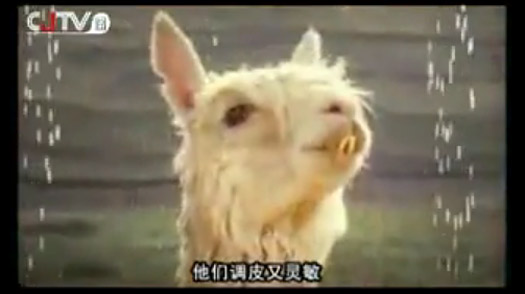
\includegraphics[width=3.7894in,height=2.1224in]{figures/chap2/chapitre2-img14.jpg}
    }
    \subfloat[Un caractère chinois composé spécialement par les internautes pour signifier cet animal mythique]{ 
        
\includegraphics[width=2.0559in,height=2.0559in]{figures/chap2/chapitre2-img15.jpg}
    }
    \caption[\textit{Caonima}: un animal mythique du web chinois]{\textit{Caonima}: un animal mythique du web chinois, d{\textquoteright}après le \textit{Grass-Mud Horse Lexicon Classics}publié par \textit{China Digital Times }(2013)}
    \label{fig:caonima}

\end{figure}

Luttant contres les crabes de rivière, le \textit{caonima }symbolise la lutte contre la censure pour un Internet libre. Apparu pour la première fois dans une vidéo virale\footnote{ \textit{Song of the Grass-Mud Horse (Cao Ni Ma), }Youtube \ \url{https://www.youtube.com/watch?v=wKx1aenJK08}, consulté le 28 Février 22:08\par }, le \textit{caonima} est un animal de la famille des camélidés (l{\textquoteright}alpaga) courant fièrement dans les prés sur une petite musique de dessin animé aux paroles entièrement réécrites pour l{\textquoteright}occasion. Littéralement {\textquotedblleft}cheval d{\textquoteright}herbe et de boue{\textquotedblright}, le mot {\textquotedblleft}caonima{\textquotedblright} (\zh{草泥马})cache en fait un double sens puisque son homophone (\zh{操你妈}) est une grossière interjection à l{\textquoteright}intention des génitrices des censeurs de Pékin. Devenu aujourd{\textquoteright}hui une véritable icône anti-censure, il n{\textquoteright}est pas rare de le croiser sur un tee-shirt ou accroché à un sac dans de nombreux endroits improbables en Chine. Comme le note très justement An Xiao Mina : \textit{{\textquotedblleft}les mèmes sont les graffitis du web censuré{\textquotedblright}} \citep{Mina2012}. Malgré le zèle des pouvoirs publics à les effacer le plus rapidement possible, ils témoignent de l{\textquoteright}existence de réalités occultées qui se manifestent souvent de manière dérisoire, grotesque et improbable, mais sont énoncées malgré tout. 

\item[Publicité et marketing viral]
\hfill \\
La popularité des services de réseaux sociaux a entra\^iné de nombreuses marques à se concentrer sur ce nouveau média pour mener leurs campagnes de publicité et de promotion. Les utilisateurs chinois sont très fortement engagés dans la création de nouveaux contenus avec 76\% des
utilisateurs chinois créant davantage de contenus qu{\textquoteright}ils n{\textquoteright}en lisent, contre seulement 20\% en France \citep{Forrester2013}. Ainsi, de nombreuses marques cherchent à concevoir des interactions en ligne utilisant les mèmes comme véhicule de messages commerciaux afin de
mettre à contribution les internautes dans la diffusion de leur marque. Une des stratégies marketing les plus répandues consiste à créer un \textit{hashtag} amusant afin d{\textquoteright}inciter les internautes à s{\textquoteright}en saisir, le partager et créer de nouveaux
contenus. La marque de préservatifs \textit{Durex} a notamment connu un large
succès avec le hashtag \textit{\#BienEtreNocturne} (en Chinois \#\zh{夜福利}) sur Sina Weibo. Drôle et un peu osé, cette campagne a généré un fort engagement des internautes, contribuant largement à la propagation du profil utilisateur et du nom de la marque \citep{Shi2012}. En récupérant les données des utilisateurs impliqués dans la diffusion, la marque peut également procéder à un travail statistique d{\textquoteright}analyse pour mieux conna\^itre les utilisateurs intéressés par ses produits.Ce type d{\textquoteright}information s{\textquoteright}avère précieuse dans un marché chinois en mouvement o\`u il existe un fort besoin pour des études de marché précises auprès de segments de populations actifs en ligne (adolescents, jeunes, classe moyenne émergente...) \citep{Bergstrom2012}. Malgré le paysage morcelé des services de réseaux sociaux chinois, les utilisateurs chinois semblent davantage enclins à suivre et interagir avec les marques que leurs homologues américains notamment\footnote{ D{\textquoteright}après Ken Hong, Sina Weibo General Marketing Manager  \url{http://adage.com/article/global-news/questions-sina-weibo-s-ken-hong-china/239508/,} consulté le 19 Février 2014 à 12:45}. 



\item[Marketing politique, soutien, pétitions]
\hfill \\
L{\textquoteright}industrie n{\textquoteright}est pas seule à s{\textquoteright}être emparée des réseaux sociaux et les grandes entités politiques ont également saisi à bras le corps ce nouveau média. Les plus brillants exemples sont sans doute les campagne menées par Barack Obama pour la présidence des Etats-Unis. L{\textquoteright}importance capitale des réseaux sociaux a placé la stratégie de diffusion virale en haut de la pile des préoccupations pour l{\textquoteright}organisation de ces deux campagnes électorales \citep{Miller2008} avec notamment l{\textquoteright}utilisation de nombreux mèmes pour fédérer les votants. Lors de l{\textquoteright}étape de campagne auprès des électeurs de l{\textquoteright}Ohio, un état décisif de la course présidentielle, l{\textquoteright}équipe d{\textquoteright}Obama a notamment fait usage d{\textquoteright}un des fameux LOCats pur mobiliser son électorat. 


\begin{figure}[htpb]
    \centering
    
\includegraphics[scale=0.8]{figures/chap2/chapitre2-img16.png}
    \caption[Lolcat utilisé lors la campagne d'Obama]{ 
        LOLCat utilisé durant la campagne d{\textquoteright}Obama en Ohio - d{\textquoteright}après \textit{Obama Campaign Deploys Cat Meme to Get Out the Vote in Ohio sur }Politicker, consulté le 28 février 2008 à 11h41 GMT+1
    } 
    \label{fig:obama-cat}
\end{figure}

En Chine également, les réseaux sociaux sont très utilisés pour la diffusion d{\textquoteright}idées lors de campagnes politiques. Les groupes nationalistes soutenus par le gouvernement se saisissent régulièrement de l{\textquoteright}actualité pour rebondir et rassembler les foules \citep{Wu2007}. Là encore, les mèmes jouent un rôle important dans l{\textquoteright}appropriation des discussions au travers de la ré-énonciation de sujets controversés en des termes différents. Les tensions grandissantes entre les habitants du territoire de Hong Kong et ceux venus de la Chine intérieure ont été notamment le sujet d{\textquoteright}une discussion intéressante par mèmes interposés. Les visites à Hong Kong sont très régulées pour les citoyens venus de Chine intérieure mais le flux massif de touristes n{\textquoteright}a néanmoins cessé de cro\^itre depuis plusieurs années avec l{\textquoteright}augmentation des quotas et l{\textquoteright}accès aux congés dans les grandes villes de la RPC. 

\begin{figure}[htpb]
    \centering
    \subfloat[Le tract original] {
        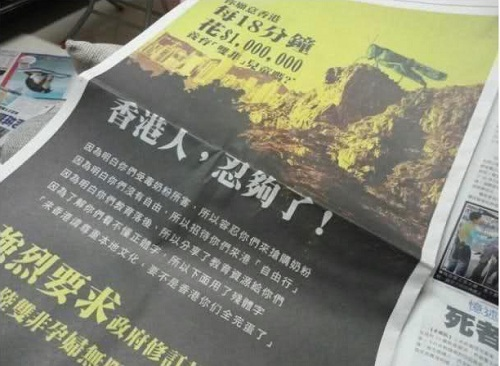
\includegraphics[width=3.3224in,height=2.4335in]{figures/chap2/chapitre2-img17.jpg}
    }
    \subfloat[Exemples de tracts réalisés par les internautes en réponse à la campagne]{
        % 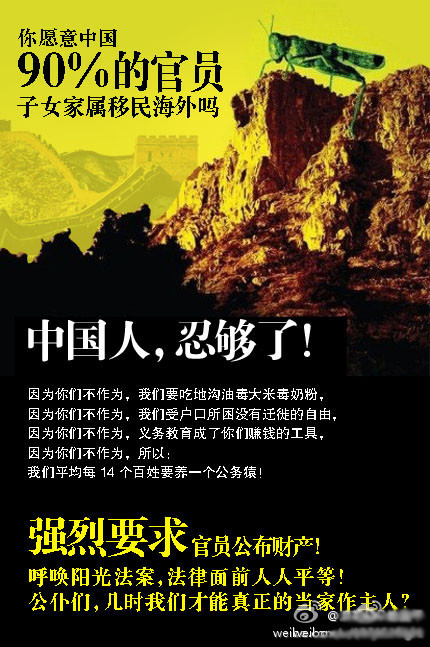
\includegraphics[width=1.4449in,height=2.178in]{figures/chap2/chapitre2-img18.jpg}
        
\includegraphics[width=1.4894in,height=2.1894in]{figures/chap2/chapitre2-img19.jpg}
        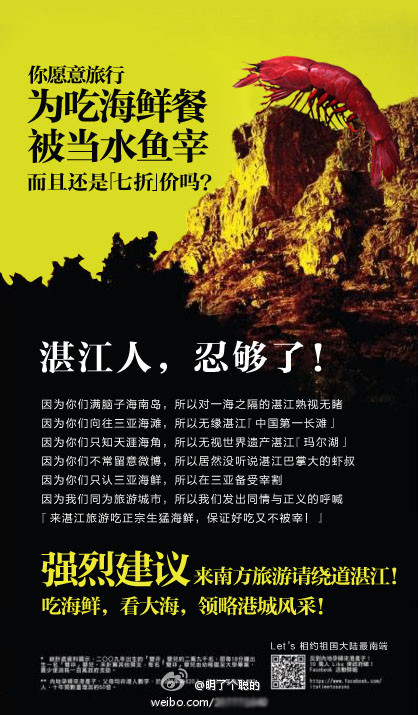
\includegraphics[width=1.2894in,height=2.2224in]{figures/chap2/chapitre2-img20.jpg}
        % 
\includegraphics[width=1.3669in,height=2.2114in]{figures/chap2/chapitre2-img21.jpg}
    }
    \caption[Détournement de tracts hongkongais anti-chinois]{Détournement de tracts hongkongais anti-chinois,d{\textquoteright}après \textit{The Civic Beat, }\url{http://reader.thecivicbeat.com/2012/03/locusts-and-pandas-and-bears-??-o-mai/} consulté le 1er Mars 2014 à 22h58}
    \label{fig:hk-tract}
\end{figure}

De nombreux chinois se rendent donc à Hong Kong pour voyager mais également profiter de la détaxe des produits de consommation et des services publics de bien meilleure qualité. La qualité des hôpitaux de la ville et l{\textquoteright}application du droit du sol dans la loi hongkongaise amènent de nombreuses jeunes mères venues de Chine à traverser la frontière pour venir accoucher à HK. Cette pratique très controversée donne à l{\textquoteright}enfant le passeport hongkongais et se monnaie à prix d{\textquoteright}or, rendant l{\textquoteright}accès aux hopitaux de plus en plus cher et attisant la colère des habitants de HK. En septembre 2012, une pétition lancée à Hongkong a cherché à recueillir des votes pour interdire l{\textquoteright}accès aux hôpitaux aux chinois venus de RPC. Un tract publié pour cette campagne a largement circulé sur le web chinois ; on pouvait y lire :\textit{ {\textquotedblleft}Habitants de Hong Kong, nous avons assez souffert ! (...) Ne nous laissons pas envahir par la vermine venue de Chine intérieure.{\textquotedblright}}  

Les internautes chinois choqués mais armés d{\textquoteright}un humour toujours très cinglant ont donc entamé une contre-campagne en proposant des versions modifiées et réécrites du dit tract. Réactions épidermiques, propos nationalistes sommaires, mais aussi critique du tourisme de masse, dénonciation de la corruption et de la mauvaise qualité des soins hospitaliers en Chine et nombreuses blagues absurdes, les adaptations et réponses singeant le tract d{\textquoteright}origine ont montré un panel d{\textquoteright}arguments et de réactions qui a permis de crever l{\textquoteright}abcés et d{\textquoteright}ouvrir un débat national sur ce problème épineux révélateur des griefs actuels des habitants de HK envers ceux de la RPC.  


\item[Fan clubs, adoration]
\hfill \\
Comme tout mass media, les réseaux sociaux possèdent une énorme quantité de contenus consacrés aux stars, à leurs vies, leurs coups durs et leurs derniers films et chansons. Développant des stratégies d{\textquoteright}envergure sur les médias chinois, de nombreuses stars internationales ont fait leur arrivée sur Sina Weibo comme notamment Brad Pitt ou Kobe Bryant. Néanmoins, leur influence reste incomparable à celles des stars originaires de Chine, de Taiwan et de Hong Kong ou bien encore de Corée du Sud, principal producteur de pop culture en Asie \citep{Martel2010}. Une des stars les plus plébiscitée dans les réseaux sociaux est pourtant une étrangère puisqu{\textquoteright}il s{\textquoteright}agit de la japonaise Sola Aoi, ex-actrice de film pornographique devenu une des 10 personnes les plus suivies sur Sina Weibo avec près de 15 millions de followers\footnote{ D{\textquoteright}après Sina Weibo \url{http://www.weibo.com/1739928273/yBJYNt7Ol,} consulté le 1 Mars 2017 à 23h11}. 

\begin{figure}[htpb]
    \centering
    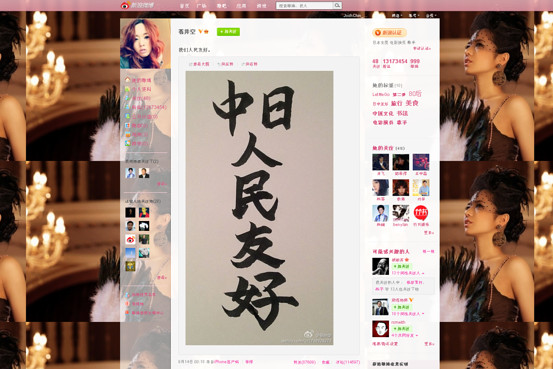
\includegraphics[scale=0.7]{figures/chap2/chapitre2-img22.jpg}
    \caption[La star du X japonaise Sola Aoi sur Sina Weibo]{Un message disant\textit{ {\textquotedblleft}Les peuples de la Chine et du Japon sont des amis{\textquotedblright} }posté par la star du cinéma pornographique japonaise Sola Aoi}
    \label{fig:pornstar-weibo}
\end{figure}

Personnalité médiatique publique, la star a depuis plusieurs années utilisé les réseaux sociaux pour nouer contact avec le public chinois qui semble bien la conna\^itre, malgré l{\textquoteright}interdiction de la pornographie en Chine. Aujourd{\textquoteright}hui retraitée du monde du X à 30 ans, Sola Aoi utilise sa popularité pour défendre une paix durable entre la Chine et le Japon. Alors que les tensions politiques exacerbées entre la Chine et le Japon ont mené à des rixes et des maltraitances envers les ressortissants dans les deux pays, elle a notamment contribué à créer un appel à la non-violence sous forme de mème \ qui a été extrêmement diffusé.  

Ainsi, les fan clubs et les stars elles-mêmes jouent un rôle important dans la création et la diffusion des mèmes, occupant une large place dans le paysage médiatique et notamment celui des réseaux sociaux. 


\item[Hoax, spam]
\hfill \\
Un des plus célèbres exemples dans ce domaine sont les emails dits de {\textquotedblleft}fraude 4-1-9{\textquotedblright} cherchant à extorquer de l{\textquoteright}argent au destinataire. Le numéro 419 correspond au numéro de l{\textquoteright}article interdisant la pratique de l{\textquoteright}escroquerie en ligne dans le code pénal nigérian. En effet, la forme la plus connue de cette arnaque est celle du {\textquotedblleft}prince nigérian{\textquotedblright} demandant un numéro de compte bancaire pour y transférer rapidement des fonds. Adaptés sous de multiples formes, ce type de messages existent également sous les réseaux sociaux sous la forme de \textit{bots}, comptes tenus par des robots postant des messages promotionnels.  

\begin{figure}[htpb]
    \begin{quote}
        I am Stella Amah 19 years of age the only daughter of late Mr Boni Amah whom was killed by the rebels that attacked our country cote d'Ivoire west Africa and took over our town (BOUAKE). I ran to Abidjan the economical capital of cote d'ivoire from were I am contacting you. Before the death of my father he told me that he has a sum of US\$9,000,000(Nine million united states dollars) kept in a private security company here in cote d'ivoire in my name as the next of kin... 
    \end{quote}
    \caption[Extrait d'un spam du type \textit{Nigerian Scam}]{
        Extrait d{\textquoteright}un {\textquotedblleft}Nigerian Scam{\textquotedblright}, d{\textquoteright}après \url{http://www.hoax-slayer.com/stella-amah-scam.shtml,} consulté le 2 Mars 2014 à 18h50
    }
    \label{fig:nigerian-scam}
\end{figure}

\end{description}

Au regard des différents exemples données ici, nous voyons qu{\textquoteright}il est difficile de classer les mèmes selon des catégories précises et qu{\textquoteright}en bien des endroits ces catégories se recoupent : les stars font de la politique alors que les politiques font dans le comique. Ainsi, il ne s{\textquoteright}agit pas de dresser des catégories rigides mais de disposer d{\textquoteright}une classification flexible pour pouvoir identifier clairement les éléments discursifs présents dans les mèmes Internet. Structure du réseau social, contenu des mèmes, formes multimédia, éléments de contexte, etc. , ces multiples dimensions des mèmes peuvent être observer empiriquement par l{\textquoteright}analyse de données.        % mèmes Internet

\addcontentsline{toc}{chapter}{Problématique et hypothèses}
\chapter*{Problématique et hypothèses}


% pages de transition entre les ch1/2 et ch3 en forme de conclusion de cette première partie de ton travail consacrée à une revue de la littérature de ton sujet et à l'aboutissement de la construction de ta problématique
% une problématique reprécisée (à l'aune de ces deux chapitres) 


\section*{Objet et problématique} 

% Contexte
L'apparition d'une industrie des contenus pour les réseaux sociaux en Chine s'inscrit dans la continuité historique du développement économique et politique du Web chinois. Le services de microblog \textit{Sina Weibo} héberge notamment de nombreuses discussions recoupant souvent blagues, faits divers, scandales politiques, marketing politique et commercial, etc.

% Objet
Parmi les nombreuses contenus échangés sur les réseaux sociaux, les \textit{mèmes Internet} offre une forme typique faisant appel à l'humour pour mobiliser des références culturelles communes. La vitesse et les vastes dimensions de leur circulation en font des objets numériques intéressants pour explorer les nouvelles interactions ayant lieu sur les plate-formes Web. 

% Thèse
\'A mi-chemin entre écriture et oralité, l’appellation de mèmes Internet recouvre pourtant des réalités diverses qui semblent procéder de motivations et de régimes d'expression forts différents. Le modèle ``viral'' souvent invoqué nous empêche de considérer l'ensemble hétéroclite de pratiques qui se déroulent lors la diffusion d'informations en ligne. Seule une observation détaillée peut nous permettre d'apporter un éclairage sur les différents régime d'expression qui préside à la production des contenus largement diffusés en ligne.

% Question(s) de recherche
Comment s'opère la diffusion des mèmes sur \textit{Sina Weibo}? A plus forte raison, quelles sont les particularités de ce type d'objets par rapport à d'autres formes de contenus plus traditionnels? Comment pouvons-nous observer ces mèmes Internet? Quelles relations entretiennent-t-ils avec le milieu numérique qui les produit? Ont-t-ils une existence territoriale?

% Problématique
Afin d'observer les différents types de contenus qui circulent sur la plate-forme de réseau social chinoise \textit{Sina Weibo}, nous allons procéder au développement d'un dispositif utilisant l'analyse et la visualisation de données. La série d'hypothèses infra accompagnera la démarche méthodologique de conception de cet outil.

\section*{Hypothèses}
\label{sec:hypotheses}

\subsubsection{La majorité des contenus circulant sur les réseaux sociaux s'apparentent largement à ceux des médias traditionnels} 

L'objet numérique communémént appelé mème Internet dans la littérature recouvre tout type de contenus qui ne s'apparente pas à ce terme. La plupart des contenus du web sont en effet des formes narratives, commerciales ou journalistiques qui pré-existent déjà bien avant l'Internet. Qu{\textquoteright}il s{\textquoteright}agisse de propagande politique ou de campagnes publicitaires, la dimension stratégique de la diffusion de contenus fait des médias un enjeu important pour tout système économique et politique. Nous pensons qu{\textquoteright}il existe de grandes similarités de diffusion entre les contenus majoritaires des services de réseaux sociaux et ceux des médias plus classiques comme la télévision ou la radio qui sont soumis à des contextes de production industrielle souvent similaires.

\subsubsection{Les mèmes sont à comprendre comme des actes d'énonciation.}

Si les formes de contenus des médias traditionnels trouvent se retrouvent sur les réseaux sociaux, la fonctionnalité nouvelle de ce type de service est la possibilité de converser en ligne.Reconductions de phénomènes anciens les mèmes Internet peuvent se comprendre comme une rumeur, un débat ou une blague à forte circulation. Ces formes archétypales nous se constituent autour de pratiques essentiellement orales, existants aujourd'hui sous le régime particulier de l'écriture en ligne. Ainsi, l'étude des  mèmes Internet nécessite de mobiliser un cadre conceptuel adéquat considérant ces actes de communication sous le régime de l'énonciation.


\subsubsection{L'analyse de la diffusion ne doit pas se contenter de l'analyse conversationnelle, mais doit mobiliser les modèles étudiant l'énonciation.}

Près d'un siècle de recherche en Sciences de la Communication nous ont permis de développer des modèles d'analyse complexe des actes de communication. Pour les échanges en ligne, nous ne pouvons nous contenter de percevoir uniquement la dimension conversationnelle sans prendre en compte les multiples aspects non-verbaux, para-verbaux ou même sémantiques qui rentrent en jeu dans les actes de communication en ligne. La parole en ligne ou hors-ligne est un acte et doit à ce titre être comprise comme tel. Une première approche que nous proposerons ici cherchera à comprendre non seulement les échanges entre utilisateurs (conversation), mais également les structures lexicales (sémantique), temporelles et géographiques qui émergent de ces échanges. L'analyse de la diffusion des mèmes nous servira de base pour discuter et comprendre comment se structurent ces actes de communication en ligne.


\subsubsection{L'analyse et la visualisation de données permettent d'établir une classification des discussions en ligne selon les structures de leurs diffusions.}

La disponibilité d'immenses volume de conversations sous la forme de vaste jeu de données issues des réseaux sociaux nous permet aujourd'hui de pratiquer de nouveaux types d'analyse pour comprendre les phénomènes entourant la communication en ligne. En analysant un jeu de données issu du réseau social Sina Weibo, nous pensons pouvoir observer des éléments particuliers et constitutifs entrant en jeu dans la diffusion des mèmes et d'autres formes de contenus en ligne. En représentant sous formes de graphes multiples appelés \textit{topogrames} différents aspects de leur diffusion, nous pouvons classifier ces discussions selon des modèles caractéristiques de conversations.

\subsubsection{La circulation des contenus sur les réseaux sociaux accroît la fragmentation du milieu numérique.}

L{\textquoteright}observation des modèles de diffusion de conversations en ligne permet de comprendre comment s'actualise le \textit{milieu numérique}, compris comme l{\textquoteright}ensemble de protocoles et outils technologiques qui les produit \citep{Hui2012}. L'étude de ces topogrammes peut également permettre d'identifier des modèle plus ouverts à la participation dites \textit{associatives }et d{\textquoteright}autres dites \textit{dissociatives} qui autorisent plus difficilement l{\textquoteright}échange. Nous pensons notamment que la segmentation de l{\textquoteright}attention suscité par la valorisation publicitaire des contenus induit un design largement dissociatif des services de réseaux sociaux, qui conduit à une fragmentation accrue des relations en ligne (structure en small worlds).

\bigskip
% le choix d'une méthodologie qui vise à explorer les hypothèses retenues

Afin d{\textquoteright}approcher ces différentes hypothèses, nous avons choisi de nous livrer à la conception d'un outil nous permettant d'analyser de larges jeux de données issus de \textit{Sina Weibo}. La dimension expérimentale de ce travail nous amènera à effectuer de nombreux choix méthodologiques que nous allons maintenant discuter.       % problématique et hypothèses

\chapter{Réflexions méthodologiques et design expérimental}

\newthought{Dans ce chapitre} nous présentons la démarche expérimentale que nous avons choisie d{\textquoteright}utiliser pour mener à bien cette recherche, ainsi que les résultats que nous avons obtenus. Nous avons choisi de nous saisir de différents outils informatiques, algorithmiques et de visualisation afin d{\textquoteright}observer les mèmes circulant sur Sina Weibo. Nous débuterons ce chapitre en discutant des implications d{\textquoteright}une méthodologie fondée sur l{\textquoteright}analyse et la visualisation de données pour une recherche en sciences sociales. Dans un second temps, nous brosserons un panorama des méthodes utilisées pour explorer les données issues des réseaux sociaux. Enfin, nous présenterons notre démarche ainsi que les résultats de cette étude. 


\section[Sciences sociales du réseau]{Sciences sociales du réseau}
Pour l{\textquoteright}empiriste, l{\textquoteright}acte essentiel de la recherche est l{\textquoteright}observation. Structure schématique faite de points et de lignes, le réseau n{\textquoteright}offre que peu de prises pour une approche empirique. Pourtant, ce concept protéiforme traverse aujourd{\textquoteright}hui les disciplines pour se retrouver au centre des débats scientifiques. Couplé à l{\textquoteright}autre grand insaisissable de l{\textquoteright}étude qu{\textquoteright}est \textit{l{\textquoteright}information, }le modèle du réseau fait la promesse de nouvelles perspectives en offrant un cadre conceptuel commun pour les sciences et de nouveaux horizons méthodologiques gr\^ace aux outils informatiques. L{\textquoteright}interrogation autour des réseaux se trouve donc plus que jamais au c{\oe}ur du devenir des sciences. 

\subsection[Le réseau comme enjeu pour l{\textquoteright}étude]{Le réseau comme enjeu pour l{\textquoteright}étude}
Durant la seconde guerre mondiale et jusqu{\textquoteright}à la fin des années 1950, les esprits les plus brillants du siècle (G\"odel, Von Neumann, Einstein..) se c\^otoient à \textit{l{\textquoteright}Institut des Etudes Avancées} de Princeton (IAS) aux USA et leurs travaux posent les bases logiques et technologiques d{\textquoteright}o\`u émerge la science informatique actuelle. Dans le domaine de la philosophie mathématique tout d{\textquoteright}abord, les interrogations amorcées par Russel dans ses \textit{Principia Mathematica }puis leur critique par G\"odel dessinent les contours d{\textquoteright}une {\textquotedblleft}machine récursive{\textquotedblright}, anc\^etre mathématique de la machine de Turing et de l{\textquoteright}ordinateur de Von Neumann. Considéré comme le père de l{\textquoteright}ordinateur, Von Neuman s{\textquoteright}exile d{\textquoteright}Allemagne pour rejoindre l{\textquoteright}IAS nouvellement fondé dès 1933 o\`u il poursuit des recherches dans le domaine de la physique nucléaire. En 1943, Von Neumann intègre le \textit{Projet Manhattan} dirigé par Oppenheimer o\`u il est chargé de superviser l{\textquoteright}immense processus de calcul nécessaire à la construction de la bombe qui s{\textquoteright}abattra sur Hiroshima le 6 A\^out 1945. C{\textquoteright}est durant cette période que Von Neumann développe l{\textquoteright}architecture encore utilisée aujourd{\textquoteright}hui comme base fondamentale du design électronique. Dans ses lectures à l{\textquoteright}Université de Yale en 1957 parues sous le titre célèbre de \textit{L{\textquoteright}Ordinateur et le Cerveau} \citep{Neumann1948}, Von Neumann identifie les différentes unités d{\textquoteright}un ordinateur : unité d{\textquoteright}arithmétique logique, unité de contr\^ole, mémoire et entrées/sorties. Les travaux teintés d{\textquoteright}ombre de ce prestigieux mathématicien font écho à ceux de l{\textquoteright}anglais Turing qui travaille également sur la question de l{\textquoteright}intelligence des machines depuis le début de la guerre. Leur correspondance témoigne du respect mutuel qu{\textquoteright}entretiennent alors les deux savants, ainsi que leurs nombreux questionnements sur la possibilité d{\textquoteright}une machine intelligente \citep{Istrail2013}. Au c{\oe}ur de leurs discussions se trouve la qu\^ete d{\textquoteright}un modèle universel capable d{\textquoteright}expliquer le fonctionnement de l{\textquoteright}activité cognitive.  

Norbert Wiener, un autre prodige des mathématiques prend également part à cette recherche. Sa théorie qu{\textquoteright}il nomme \textit{cybernétique }place la notion d{\textquoteright}information au c{\oe}ur de la réflexion sur le fonctionnement des systèmes : \textit{{\textquotedblleft}Information is information, not matter or energy{\textquotedblright}} \citep{Neumann1948}, p. 155). Utilisant les concepts de bruit, de messages et de \textit{feedbacks}, il jongle entre mathématiques appliquées et sciences cognitives pour comprendre les phénomènes de transmission de signaux complexes. Dans une lettre du 29 Novembre 1946, Von Neumann écrit à Wiener que l{\textquoteright}étude du cerveau {\textquotedblleft}\textit{the most complicated object under the sun, litterally}{\textquotedblright} nécessite de poursuivre une réflexion transverse à de multiples disciplines scientifiques \citep{Masani1990}. Depuis le début de cette m\^eme année 1946, les {\textquotedblleft}conférences cybernétiques{\textquotedblleft} aussi connues sous le nom de {\textquotedblleft}conférences Macy{\textquotedblright} ont débuté à New York dans le but de définir \textit{{\textquotedblleft}une science général de l{\textquoteright}esprit humain{\textquotedblright}}\footnote{ Foundation for Cybernetics, The Macy Conferences \url{http://www.asc-cybernetics.org/foundations/history/MacySummary.htm} consulté le 10 Mars 2014 à 16h16 GMT+1}. Regroupant physiciens, cogniticiens, biologistes, anthropologues et linguistes, ces conférences sont l{\textquoteright}objet de nombreuses publications dont \textit{The Human Use of Human Beings} \citep{Wiener1988} qui propose d{\textquoteright}étudier la société en considérant les communications entre hommes et machines. Le travail mené lors de ces conférences est souvent considéré comme la pierre fondatrice du champ des études sur la communication \citep{Breton1997, Winkin1981}. Quelques années plus tard, McLuhan et son idée controversée de \textit{village global} \citep{McLuhan1962} amènent un large auditoire autour des {\oe}uvres de Wiener et l{\textquoteright}étude des modes de communication. Progressivement se constitue un champ épistémologique pour l{\textquoteright}étude de l{\textquoteright}information dont la définition reste encore aujourd{\textquoteright}hui un enjeu important \citep{Wolton1997}. En France, les Sciences de l{\textquoteright}Information et de la Communication se sont principalement structurées autour de la critique des médias \citep{Mattelart1986, Debray1991} dans une tradition européenne déjà bien installée \citep{Adorno2005}. Aux Etats-Unis, les \textit{cultural studies }\citep{Hall2003} s{\textquoteright}interrogent davantage sur l{\textquoteright}économie politique des symboles et trouvent leurs lettres de noblesse dans les \textit{media studies, }aujourd{\textquoteright}hui devenue une discipline universitaire reconnue en Angleterre et aux USA. Toutefois, l{\textquoteright}émergence d{\textquoteright}un \textit{{\textquotedblleft}paradigme communicationnel{\textquotedblright} }\citep{Bougnoux1993} nécessite un dialogue pas toujours évident entre les différentes disciplines constituées autour de l{\textquoteright}étude des pratiques de l{\textquoteright}information et de la communication : sociologie des médias, études des systèmes d{\textquoteright}information, informatique, sciences de l{\textquoteright}information et de la communication, etc.  


Alors que le programme fixé par la cybernétique a pour ambition  d{\textquoteright}explorer les structures, possibilités et  contraintes des systèmes communicants, l{\textquoteright}image  fermée et cyclique du système devient rapidement trop étriquée  pour une réflexion sur les relations en pleine expansion. Deleuze et  Guattari proposent dans l{\textquoteright}introduction de leur livre  \textit{Milles Plateaux} \citep{Deleuze1972} de s{\textquoteright}éloigner de  l{\textquotesingle}arborescence classique du système auto-suffisant  pour envisager les liens entre sujets et objets sous la forme ouverte  et combinatoire du \textit{rhizome. }Le rhizome se définit par son  caractère non-fini et fait de l{\textquoteright}étude des  causalités un phénomène contextuel aux spécificités pas  forcément reproductibles. Imperméable à la catégorisation et  aux classifications ordonnées, l{\textquoteright}objet  d{\textquoteright}étude in-formé devient \textit{open-ended},  moment donné à voir et état unique d{\textquoteright}un ensemble  plus vaste. La vérité ou la validité n{\textquoteright}est donc  plus à découvrir dans l{\textquoteright}analyse, mais plut\^ot dans  l{\textquoteright}articulation des contingences entre objets et  environnements dont se saisit le champ émergent des études sur la  complexité \citep{Morin1990}. Dans le m\^eme temps, les progrès de  l{\textquoteright}intelligence artificielle et de la robotique viennent  également questionner notre définition du vivant face à ces  nouveaux \^etres \citep{Hofstadter1999}. Le modèle du \textit{réseau  }vient à son tour in-former la pensée scientifique comme un nouvel  \textit{episteme }foucaldien offrant une grille de lecture des faits  sociaux renouvelée \citep{Castells1989, Latour1996}.  Aujourd{\textquoteright}hui, la structuration d{\textquoteright}un  champ de recherche cohérent et multi-disciplinaire autour de  l{\textquoteright}étude des réseaux reste un enjeu important pour  le monde de la recherche \citep{Brandes2013}. Cette considération  pour la complexité des phénomènes permet en effet  d{\textquoteright}imaginer une approche scientifique qui atténuerait  les liens entre des disciplines dont le dialogue parfois difficile est  néanmoins nécessaire, afin de mener vers une réconciliation des  sciences humaines, des sciences naturelles et des sciences du vivant  o\`u cohabiteraient  \textit{{\textquotedblleft}l{\textquoteright}étude des organismes, des organes et des organisations{\textquotedblright} }\citep{Morin1990}


\subsection[Code, données et les nouveaux outils de l{\textquoteright}écriture scientifique ]{Code, données et les nouveaux outils de l{\textquoteright}écriture scientifique }
Les objets ouverts et mal définis du réseau posent néanmoins la question d{\textquoteright}une continuité avec le projet aristotélicien d{\textquoteright}une compréhension du monde par le savoir analytique. La considération d{\textquoteright}un objet comme moment du réseau rend caduque l{\textquoteright}idée de sa définition \textit{a priori, }en dehors des relations qu{\textquoteright}il entretient avec son environnement. A l{\textquoteright}inverse, une définition des objets entre origine, fonction et destination ne devrait pas éluder non plus la réflexion ontologique autour de son \textit{\^etre}. Le philosophe américain William James propose une méthode qu{\textquoteright}il nomme \textit{empirisme radical }o\`u l{\textquoteright}existence des objets doit \^etre considérée par le prisme de l{\textquoteright}expérience \citep{James1912}\textit{. }L{\textquoteright}expérience, m\^eme scientifique, existe dans un contexte, un lieu, un temps, un moment, une succession d{\textquoteright}étapes, et c{\textquoteright}est cet ensemble qui nous permet de percevoir les phénomènes étudiés. Si l{\textquoteright}acte essentiel de l{\textquoteright}empiriste et du philosophe est l{\textquoteright}observation, alors elle doit \^etre radicale dans son honn\^eteté et accepter l{\textquoteright}expérience dans son unicité dont de nombreux facteurs sont non-reproductibles. Cette question de l{\textquoteright}expérience et de sa reproductibilité est depuis toujours au c{\oe}ur du débat sur les sciences et se pose comme un des ressorts fondamentaux du savoir scientifique. Les sciences dites {\textquotedblleft}dures{\textquotedblright} comme la physique, la biologie, l{\textquoteright}informatique ou m\^eme la géologie valident leurs hypothèses gr\^ace à l{\textquoteright}usage extensif d{\textquoteright}appareillages multiples devenus une clé de la reproductibilité des expériences. Du simple microscope à l{\textquoteright}accélérateur du CERN, la méthodologie d{\textquoteright}observation est pour ces disciplines souvent indissociable de la technologie. Le travail de la recherche et de la preuve s{\textquoteright}articule ici autour des trois p\^oles de la théorie, de l{\textquoteright}expérience et de la méthode conditionnée à la technique.  

\begin{figure}
    \centering
    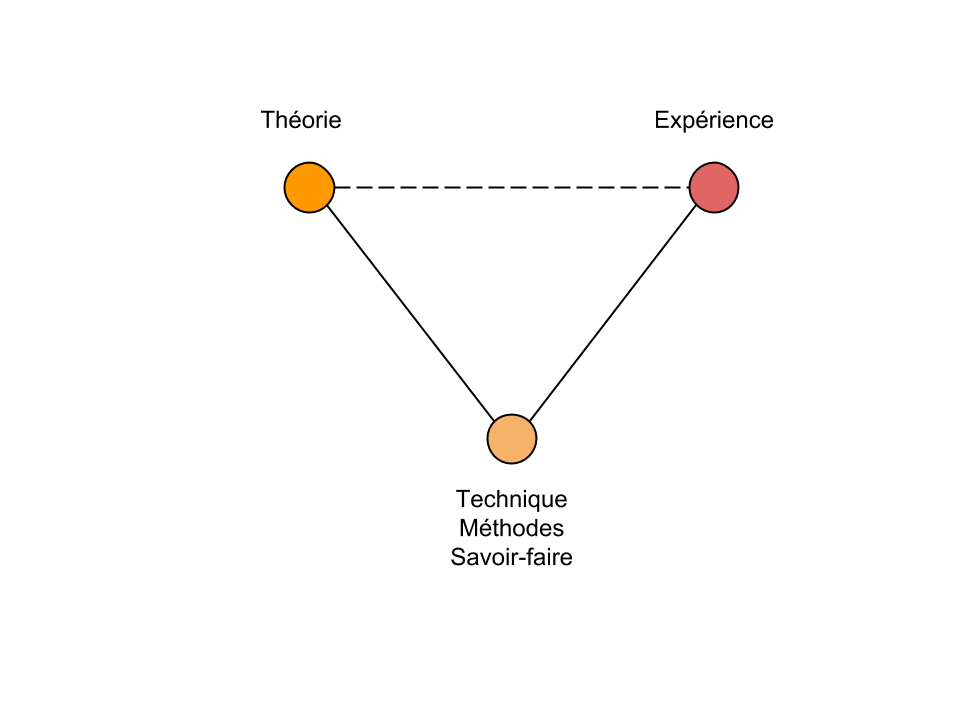
\includegraphics[width=5.0559in,height=3.7894in]{figures/chap3/chapitre3-img1.png}
    \caption[Triptyque des pratiques scientifiques]{Triptyque des pratiques scientifiques}
\end{figure}


En sciences sociales néanmoins, la tension entre la théorie (les concepts), l{\textquoteright}expérience (le terrain) et la méthodologie s{\textquoteright}articule plus rarement autour d{\textquoteright}outillages élaborés. Les \ réflexions sur la méthodologie en sciences sociales portent plus largement sur des argumentations conceptuelles o\`u le langage lui-m\^eme est considéré comme l{\textquoteright}outil premier ou encore de nombreuses réflexions éthiques sur l{\textquoteright}impact des pratiques d{\textquoteright}observation dans le cadre de l{\textquoteright}anthropologie notamment. En France, l{\textquoteright}intér\^et constant porté à l{\textquoteright}utilisation des différentes formes de technologie en sciences humaines s{\textquoteright}est souvent constitué autour de la critique de méthodologies quantitatives très répandues outre atlantique - la statistique en sociologie, l{\textquoteright}étude comportementaliste en psychologie ou le film ethnographique \citep{Becker1996}. Comme le note justement Latour, la qu\^ete de légitimité des Sciences Sociales s{\textquoteright}est souvent traduit par une capacité à se procurer et traiter des données : \textit{{\textquotedblleft}Sociology has been obsessed by the goal of becoming a quantitative science.{\textquotedblright}} \citep{Latour2003}. Pourtant, il serait illusoire de corréler la quantité de données à une quelconque objectivité de la démarche scientifique, tant les démarches et outils nécessaires pour la collecte sont en soi autant de biais importants. La question de la réussite des études utilisant les Big Data semble davantage corrélée à la capacité d{\textquoteright}une approche méthodologique forgée dans un échange interdisciplinaire et des pratiques renouvelées de l{\textquoteright}écriture. La complexité des questions abordées lors du traitement des données, non seulement technologique mais aussi dans les interrogations sur la légitimité de leur existence, leur utilisation et leur provenance \citep{Boyd2011} rendent nécessaire la discussion entre de multiples connaissances. Aujourd{\textquoteright}hui, l{\textquoteright}utilisation de l{\textquoteright}ordinateur conditionne l{\textquoteright}écriture scientifique de l{\textquoteright}étude de terrain, la prise de notes, la rédaction ou la publication et se présente ainsi comme un impératif méthodologique pour la réflexion et le travail en sciences humaines et sociales \citep{Wieviorka2013}. L{\textquoteright}appareillage projeté au centre de la pratique quotidienne du chercheur vient modifier le travail de réflexion sur les phénomènes étudiés et s{\textquoteright}accompagne de multiples contraintes. La prise en main de ce nouvel \textit{{\textquotedblleft}instrument intellectuel{\textquotedblright} }\citep{Guichard2014} passe par une lente alphabétisation aux langages des machines. L{\textquoteright}angoisse latente du {\textquotedblleft}bug{\textquotedblright} n{\textquoteright}est pas apaisée par les rares techniciens présents dans les centres de recherche en sciences humaines, souvent déjà dépassés par la diversité des demandes technologiques. L{\textquoteright}écriture, savoir-faire indispensable de la recherche, possède une nouvelle matérialité dans les disques durs produisant une dépendance accrue aux réseaux d{\textquoteright}ordinateurs. Cette empreinte {\textquotedblleft}digitale{\textquotedblright} laissée par les calculateurs sur les pratiques scientifiques n{\textquoteright}est ni anodine ni révolutionnaire et s{\textquoteright}inscrit dans la longue tradition des cultures de l{\textquoteright}écrit qui déjà bien avant les moines copistes \textit{{\textquotedblleft}combinent les gestes de la main et les opérations de la pensée.{\textquotedblright}} \citep{Jacob2011}  

Tim Berners-Lee, considéré comme l{\textquoteright}inventeur du World Wide Web et du Web Sémantique définit la constitution d{\textquoteright}un réseau mondial des savoirs comme un projet d{\textquoteright}\textit{{\textquotedblleft}ingénierie philosophique{\textquotedblright} }\citep{Halpin2014}. Mi-philosophe mi-ingénieur, le chercheur contribuant à ce réseau de savoir doit donc \^etre en capacité de conna\^itre les protocoles et les langages pour y accéder et s{\textquoteright}y mouvoir aisément. La méthode scientifique s{\textquoteright}écrit notamment avec de nouvelles formulations (fonctions, algorithmes, code...). Les données générées par les usages d{\textquoteright}un nombre croissant de machines communicantes et productrices d{\textquoteright}information, souvent désignées par le concept {\guillemotleft} valise {\guillemotright} de Big Data \citep{Lohr2012} offrent des possibilités nouvelles pour l{\textquoteright}étude en sciences sociales. L{\textquoteright}analyse de ces vastes jeux de données s{\textquoteright}accompagne également de nouveaux impératifs et questionnements sur l{\textquoteright}observation des phénomènes humains qu{\textquoteright}ils représentent. à la fois barrière et opportunité, une difficulté majeure réside dans le discernement nécessaire entre praxis des outils informatiques, fascination pour ces outils et réflexions pertinentes sur la qualité des méthodes employées. Le traitement quantitatif par ordinateur permet d{\textquoteright}extraire de nombreuses connaissances utiles de jeux de données parfois très importants mais n{\textquoteright}assure pas pour autant la qualité des résultats. Une bonne compréhension de la provenance et des méthodes de collection des données est nécessaire afin d{\textquoteright}identifier des algorithmes de traitements intéressants, adaptés et efficaces parmi ceux disponibles \citep{Rajaraman2011}. Les méthodologies d{\textquoteright}exploration et de recherche utilisant le {\textquotedblleft}Big Data{\textquotedblright} comme source nécessitent la mise en {\oe}uvre d{\textquoteright}une ingénierie complexe soutenue par une connaissance des technologies nécessaires à l{\textquoteright}analyse de données. L{\textquoteright}algorithmique, la statistique, l{\textquoteright}informatique mais également la cartographie et le design graphique doivent se conjuguer pour permettre de produire des résultats à la fois intéressants et fiables. Ce travail d{\textquoteright}hypothèses et de vérifications pour l{\textquoteright}analyse de données doit réunir de nombreuses compétences. La définition de la problématique la plus adaptée nécessite une connaissance aig\"ue du terrain et des outils et algorithmes qui seront articulés au sein d{\textquoteright}un système ingénierique parfois très complexe. Le design et la lecture d{\textquoteright}algorithme pour le \textit{{\textquotedblleft}data mining{\textquotedblleft}} sont donc les clés pour le travail du chercheur confronté aux données. Néanmoins, ces algorithmes ne devraient \^etre que la traduction de questions formulées gr\^ace à une connaissance aig\"ue des problématiques du contexte et des objets étudiés - notamment pour identifier les données manquantes. La {\textquotedblleft}science des données{\textquotedblright} promet donc d{\textquoteright}apporter un véritable renouveau des méthodes et des résultats scientifiques, au prix d{\textquoteright}un travail soutenu pour faire face à ces changements d{\textquoteright}habitudes et de langages. Les applications statistiques du {\textquotedblleft}big data{\textquotedblright} permettent aujourd{\textquoteright}hui une fiabilité accrue des prédictions par l{\textquoteright}augmentation du volume des corpus traités \citep{Breiman2001}. Le domaine de l{\textquoteright}intelligence artificielle (AI) a grandement bénéficié de l{\textquoteright}accroissement de la capacité de traitement des données notamment pour la prédiction gr\^ace au techniques dites de \textit{machine learning}. Néanmoins Peter Norvig, directeur de recherche chez Google, reconnait lui-m\^eme : {\textquotedblleft}\textit{We could draw this curve: as we gain more data, how much better does our system get? And the answer is, it{\textquoteright}s still improving---but we are getting to the point where we get less benefit than we did in the past.{\textquotedblright} }\citep{Somers2013}. Comme le note Douglas Hofstadter, un des pairs de l{\textquoteright}Intelligence Artificielle à propos du super-ordinateur qui venait de battre Kasparov aux échecs : \textit{{\textquotedblleft}Okay, Deep Blue plays very good chess---so what? Does that tell you something about how we play chess? No. Does it tell you about how Kasparov envisions, understands a chessboard?{\textquotedblright} }\citep{Somers2013}.  

En effet, ces pratiques méthodologiques doivent réussir à s{\textquoteright}inscrire dans la continuité de l{\textquoteright}historicité et des exigences des disciplines. La portabilité des méthodes et la disponibilité des données sont encore des questions centrales et non-résolues. En sciences sociales notamment, les services de réseaux sociaux en ligne offrent de très larges corpus dont l{\textquoteright}utilisation est régie par les exigences commerciales des sociétés privées qui les détiennent. L{\textquoteright}analyse des données issues de service de réseaux sociaux en ligne est pourtant un champ d{\textquoteright}études en rapide expansion \citep{Nettleton2013}. Pourtant, le débat sur la validité des éclairages apportés par l{\textquoteright}analyse des données issues des services de réseaux reste encore largement ouvert et nous entendons dans ce travail de recherche y contribuer.  

\subsection[Visualisation et espace perceptif pour l{\textquoteright}information]{Visualisation et espace perceptif pour l{\textquoteright}information}

Face à de larges volumes de données, un des grands enjeux est d{\textquoteright}en restituer une forme intelligible afin d{\textquoteright}identifier des tendances ou des motifs particuliers. La visualisation permet de produire une lecture particulière de parties intéressantes et intelligibles d{\textquoteright}un jeu de données \citep{Cairo2013}. Définie comme \textit{{\guillemotleft}~a process that transforms data, information, and knowledge into a form that relies on the human visual system to perceive its embedded information.{\textquotedblright}} \citep{Graffieti2010}, la visualisation introduit la question du design visuel au c{\oe}ur de la problématique d{\textquoteright}analyse \citep{Wesolowsky1992}. La visualisation correspond à une série d{\textquoteright}actions qui résulte dans la production de marqueurs visuels (points, ligne, aires, surface, volume) avec comme étapes la définition de leurs propriétés rétiniennes (couleur, taille, texture, etc.) et leur positionnement dans l{\textquoteright}espace visuel \citep{Card1997}. Dans son travail, Engelhardt \cite{Engelhardt2007} s’attache   à définir les bases d{\textquoteright}une grammaire de la visualisation en commen\c{c}ant par en identifier les formes syntaxiques :  
\begin{enumerate}
\item les objets graphiques montrés (ex. point, flèche, pictogramme, etc.), 
\item l{\textquoteright}espace graphique donnant sens à l{\textquoteright}organisation des objets (ex. systèmes de coordonnnées géographiques, timeline, etc.), 
\item les propriétés graphiques des objets (couleurs, tailles, etc.), 
\item l{\textquoteright}organisation des objets en différentes catégories (ex. cadre, liens, légendes, etc.). 
\end{enumerate}

Ces choix forment une t\^ache importante dont l{\textquoteright}enjeu n{\textquoteright}est pas seulement visuel, mais se joue également dans le champ de la représentation o\`u les objets sont donnés à voir et par là-m\^eme donnés à comprendre. Les travaux sur l{\textquoteright}apparition de la perspective dans la Renaissance italienne ont montré comment l{\textquoteright}espace de la représentation visuelle fait écho aux changements sociétaux profonds de l{\textquoteright}époque \citep{Raynaud2005}. Au-delà d{\textquoteright}une simple technique picturale, les {\oe}uvres des peintres du Quattrecento témoignent de changements profonds dans la perception : l{\textquoteright}espace perceptif se structure désormais autour du sujet et \ de son {\textquotedblleft}point de vue{\textquotedblright} qui construit l{\textquoteright}ensemble de la représentation \citep{Damisch1999}. Empreinte de rationalité, la perspective construit comme au thé\^atre un espace de représentation centré autour du spectateur. En 1639, le mathématicien Desargues modélise les notions intuitives de perspective et d{\textquotesingle}horizon gr\^ace à la géométrie projective qui permet d{\textquoteright}étudier les propriétés inchangées des figures lors de leur projection. Cette géométrie d{\textquoteright}un genre nouveau se structure autour du \textit{plan projectif}, élément topologique qui \textit{{\textquotedblleft}rassemble en une seule surface l{\textquoteright}imagination de tous les points de vue possible{\textquotedblright} }\citep{Petit1999}. En construisant un plan géométrique fondé sur le point de vue, de nouveaux \^etres géométriques aux propriétés étranges voient le jour, dont l{\textquoteright}existence logique force notre représentation classique : la bande de M\"obius ne possède qu{\textquoteright}une seule face et il est impossible de distinguer l{\textquoteright}intérieur de l{\textquoteright}extérieur d{\textquoteright}une bouteille de Klein. Dans ces surfaces dites \textit{unilatères}, le local est traversé en tout point par un tout global. Nous ne pouvons pas traverser puisque nous somme toujours sur la m\^eme face. Ni bord, ni extérieur, ni intérieur, le plan projectif apporte des éléments de réponses conceptuelles aux limites des la représentation dans l{\textquoteright}espace.

Dans le contexte de systèmes et de réseaux complexes, la visualisation de données structure l{\textquoteright}espace perceptif afin de construire une scène à \textit{n }dimensions dont l{\textquoteright}enjeu est la recherche d{\textquoteright}un {\textquotedblleft}point de vue{\textquotedblright} pour l{\textquoteright}étude\textit{. }Alors que la perspective prend pour parti de matérialiser le sujet au centre de la représentation par des points de fuite, la visualisation de données cherche elle à utiliser les objets comme dimensions du champ de la représentation, en structurant souvent l{\textquoteright}espace autour de quantités. Néanmoins, la place du spectateur / utilisateur dans la visualisation reste un des enjeux majeurs encore à explorer. En élaborant sa {\textquotedblleft}méthode graphique{\textquotedblright} , J.E. Marey \citep{Marey1885} utilise la photographie pour créer un nouvel espace de représentation du mouvement et observer des phénomènes jusqu{\textquoteright}ici invisibles. Si la temporalité de l{\textquoteright}écrit ou de la voix est avant linéaire, l{\textquoteright}espace visuel permet de manier le réel pour le décomposer en actes logiques. Charcot cherche dans les images de l{\textquoteright}hystérie des témoignages de la folie et procède à la mise en scène de ses patients dans ce nouvel espace de représentation ouvert par la photographie \citep{DidiHuberman2012}.

La visualisation scientifique se prévaut donc d{\textquoteright}une existence avant tout pratique dont le premier objectif serait de \textit{{\guillemotleft}~to effectively convey information~{\guillemotright}} \citep{Kelleher2011}. Son caractère syncrétique et sa capacité à résumer une large masse d{\textquoteright}information rapidement en font un des plus importants éléments de la publication en science notamment pour sa diffusion et la facilitation d{\textquoteright}accès à une connaissance \citep{Ware2004}. Dans sa sémiologie graphique, Bertin \citep{Bertin1977} distingue deux usages majeurs des graphiques de visualisation : 1) un moyen de communiquer des informations (dans le cas o\`u l{\textquoteright}information a déjà été comprise) 2) un moyen visuel de résoudre des problèmes logiques (quand le graphique est utilisé comme support de lecture et de manipulation d{\textquoteright}informations). Ces deux caractéristiques peuvent coexister dans certaines pièces mais la transition entre les deux nécessite souvent un travail important de restructuration visuelle. Dans le traitement et la visualisation des données \textit{l{\textquoteright}interface }joue un r\^ole primordial. On peut désormais agir sur la deuxième catégorie de Bertin pour mieux explorer le sens \citep{Weissberg2007}. Manovich montre comment l{\textquoteright}interface définie comme \textit{{\textquotedblleft}the ways to represent ({\textquoteleft}format{\textquoteright}) and control the signal.}{\textquotedblright} \citep{Manovich2013}. Ce formatage nouveau de l{\textquoteright}information induit des changements dans la pratique de la lecture qui, toujours selon Manovich, s{\textquoteright}apparenterait davantage à de la reconnaissance de \textit{pattern}, symbolisé par l{\textquoteright}usage de l{\textquoteright}ic\^one et du menu en design d{\textquoteright}interface. Ainsi si l{\textquoteright}interface contraint la lecture, la prise en compte des formes narratives (les \textit{patterns} de Manovich) prend une grande importance quand il s{\textquoteright}agit de concevoir une visualisation d{\textquoteright}information. L{\textquoteright}usage des signes graphiques doit se faire avec une connaissance des usages de l{\textquoteright}interface, afin de recréer la coopération textuelle des r\^oles de lecteur et de designer/auteur nécessaire pour la production un sens \citep{Eco1985}. La \textit{citizen science} ou encore \textit{night science} a fait de l{\textquoteright}interface un paradigme en utilisant la visualisation pour amener un grand nombre de collaborateurs à explorer et analyser de vastes jeux de données en effectuant des t\^aches simples \citep{Silvertown2009}. Le projet \textit{Eyewire} permet à des internautes de contribuer à la classification d{\textquoteright}images du cerveau humain en vue de la réalisation d{\textquoteright}un modèle 3D \citep{Seung2012}. Utilisant des scans de tranches de 1mm réalisés par l{\textquoteright}institut Max Planck, la modélisation 3D d{\textquoteright}un cerveau complet promet une belle contribution pour la découverte des fonctionnements cognitifs. Néanmoins, la t\^ache est colossale et nécessiterait plusieurs années pour une équipe classique de scientifiques. \textit{Eyewire} propose donc une interface web o\`u un simple jeu de coloriage permet d{\textquoteright}identifier les neurones et de contribuer ainsi au dessin du modèle 3D.

Cartes, code ou graphiques, les nouveaux outils numériques participent donc à structurer de nouvelles pratiques de l{\textquoteright}espace numérique gr\^ace à la construction de nouvelles représentations. 

\section[L{\textquoteright}analyse de la diffusion sur les réseaux sociaux]{L{\textquoteright}analyse de la diffusion sur les réseaux sociaux}

Nous allons maintenant regarder comment l{\textquoteright}analyse des données des services de réseaux sociaux en ligne (SNA) peut permettre d{\textquotesingle}interroger les pratiques des technologies numériques pour mieux en comprendre les tenants. 


\subsection[Anatomie d{\textquoteright}un réseau social]{ Anatomie d{\textquoteright}un réseau social}

La représentation des relations sociales sous forme de graphe trouve son origine dans les travaux des psychologues allemands de la \textit{gestalt }durant les années 1920-1930 \citep{Scott1988}\textit{. }S{\textquoteright}inspirant des études sur le cerveau, le psychologue J. L. Moreno s{\textquoteright}applique notamment à comprendre les principes organisationnels holistiques des groupes humains et fonde la sociométrie avec comme objectif la qualification et la quantification des relations sociales \citep{Moreno1938}. Moreno cherche à identifier et isoler des leaders de groupes sociaux définis en étudiant l{\textquoteright}asymétrie ou la réciprocité de leurs choix et fréquentations amicales. Cherchant des moyens de représenter les tendances à l{\textquoteright}auto-organisation qu{\textquoteright}il observe, il cartographie les relations directes et indirectes entre personnes sous forme de \textit{sociogrammes}. Les anthropologues s{\textquoteright}emparent rapidement de ce type d{\textquoteright}outils pour comprendre les formes tribales (Lundberg, 1936) et l{\textquoteright}émergence progressive de la topologie comme domaine important des mathématiques vient définir de nouveaux types de relations entre objets disparates, avec notamment la théorie des graphes qui donne à l{\textquoteright}étude des réseaux ses modèles logiques \citep{Harary1977}. Milgram \citep{Travers1969} voit les relations humaines comme autant de petits mondes (\textit{small-worlds)} connectés entre eux. Granovetter s{\textquoteright}intéresse à l{\textquoteright}importance des relations ténues et lointaines (\textit{weak ties}) dans l{\textquoteright}acquisition d{\textquoteright}informations importantes \citep{Granovetter1973}. L{\textquoteright}influence de la théorie des graphes amène notamment les sociologues à expérimenter de nouveaux modèles venus de la physique ou de la biologie, en proposant de nouvelles pratiques comme celle de la simulation sociale \citep{Epstein1996}. 


La matérialité de l{\textquoteright}image du \textit{graphe} structure la représentation du réseau social. Dans la littérature concernant les réseaux, les notions de graphe et de réseau sont interdépendantes et la théorie des graphes sert notamment de systèmes de notation pour la mise en équation des réseaux \citep{Nettleton2013}. Si cette structure point-ligne semble toutefois rev\^etir une limite de taille pour la description de phénomènes humains (comment en effet réduire les relations humaines à une simple ligne?), elle semble néanmoins aujourd{\textquoteright}hui encore difficile à dépasser.

\begin{figure}
    \centering
    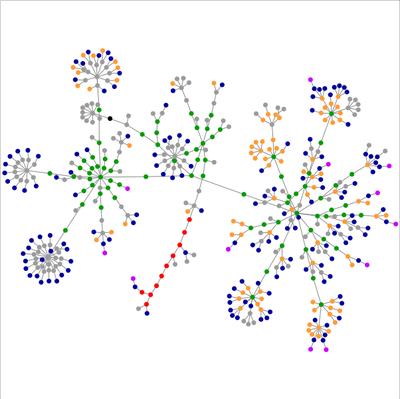
\includegraphics[width=4.178in,height=4.1449in]{figures/chap3/chapitre3-img2.png}
    \caption{Représentation d'un réseau sous forme de graphes.}
\end{figure}


Un réseau considéré comme graphe, noté \textit{G}, se compose d{\textquoteright}un ensemble de nodes ou vertices (les points) et de liens ou edges (les traits). On représente ainsi un graphe sous la notation \textit{G(V,E)} o\`u \textit{V }est l{\textquoteright}ensemble des nodes du réseau et \textit{E} l{\textquoteright}ensemble des liens\textit{ }décrivant leurs relations. \textit{E }décrit les relations entre les nodes qui peuvent \^etre directionnelles (paires de vertices ordonnées) dans le cas d{\textquoteright}un graphe \textit{orienté }ou accompagné de valeurs particulières dans un graphe dit \textit{pondéré. }Les relations ainsi exprimées portent sur un aspect unique, quantifiable et isolable. La prise en compte de facteurs multiples, comme notamment l{\textquoteright}espace physique, le temps, mais également les multiples réseaux de relations qui peuvent exister entre deux acteurs nous amènent à considérer un graphe disposant de multiples couches \textit{(}\textit{multi-layered)} pour décrire l{\textquoteright}ensemble des groupes de relations. Imaginons un graphe de personnes \textit{G (V,E}\textit{\textsubscript{n}}\textit{)} o\`u \textit{V }sont les vertices représentant les personnes et \textit{E}\textsubscript{n} un nombre \textit{n }d{\textquoteright}ensemble de liens\textit{ }décrivant chaque type de relations spécifiques. Le graphe ci-dessous montre un exemple d{\textquoteright}un graphe multi-couche o\`u \textit{E}\textit{\textsubscript{1}} est l{\textquoteright}ensemble des relations amicales, \textit{E}\textit{\textsubscript{2}}\textsubscript{ }les relations de travail et \textit{E}\textit{\textsubscript{3}}\textsubscript{ }les relations familiales.

\begin{figure}
    \centering
    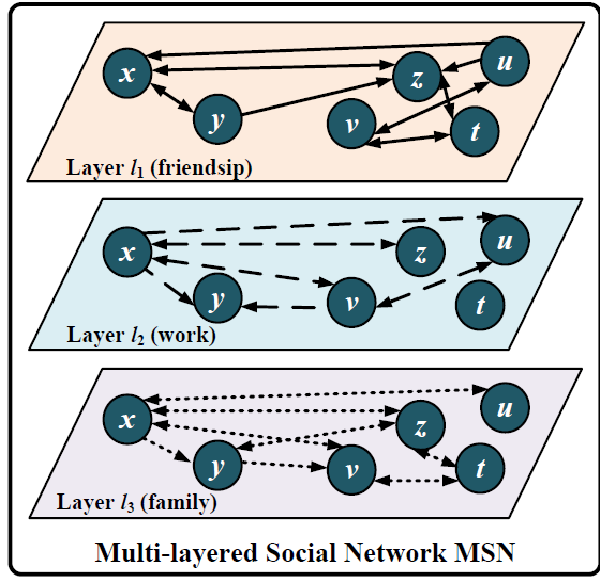
\includegraphics[width=3.8004in,height=3.6894in]{figures/chap3/chapitre3-img3.png}
    \caption [réseau social multi-couches] {Un réseau social multi-couches, d{\textquoteright}après (Brodka\&al., 2013)}
\end{figure}

Nous pouvons ainsi décrire différents jeux de relations entre un jeu d{\textquoteright}acteurs finis, permettant notamment de mieux comprendre les relations entre ses différentes dimensions. Si cette approche résout momentanément la question des \textit{n }dimensions à considérer \citep{Brodka2013} elle augmente également la complexité du graphe et la possibilité d{\textquoteright}erreurs de lecture ou de typage des relations.

Afin de mieux comprendre l{\textquoteright}organisation d{\textquoteright}un réseau, nous disposons de plusieurs mesures~pour décrire les relations et le r\^ole des différents acteurs :

\begin{itemize}
\item \textit{Degree} : (\textit{degré} ou \textit{valence}) mesure le nombre de connections d{\textquoteright}un n{\oe}ud dans un réseau. Cette valeur indique souvent une possibilité, le potentiel d{\textquoteright}un node donné à interagir avec d{\textquoteright}autres.  
\item \textit{Closeness : }(proximité) mesure la facilité d{\textquoteright}un node à se connecter à un autre. Dans un réseau en ligne, on calcule la proximité en estimant la distance la plus courte entre un node et un autre. 
\item \textit{Betweenness} (\textit{centralité}) mesure le degré d{\textquoteright}importance d{\textquoteright}un node dans le réseau en prenant en compte le nombre de nodes dépendant de lui pour
établir une connection entre eux. La centralité représente la capacité à bloquer ou laisser filtrer l{\textquoteright}accès à certaines parties du réseau. Dans une entreprise par exemple, la secrétaire du CEO a par exemple une très haute centralité.
\end{itemize}

En observant ces différentes mesures, nous pouvons définir différentes structures types pour chaque réseau. La distribution des degrés dans le graphe permet notamment de comprendre les modèles qui régissent les connexions entre les nodes. L{\textquoteright}exemple le plus simple est le \textit{random network, }réseau o\`u les acteurs sont connectés de manière entièrement aléatoire. Un réseau dont le degré de distribution correspond à une loi de puissance est appelé \textit{scale-free network. }Un réseau dont seulement quelques nodes possèdent une centralité élevée et dont la structure d{\textquoteright}ensemble est faite de groupes ou \textit{clusters} interconnectés et appelé un \textit{small-world network}.

\begin{figure}
    \centering
    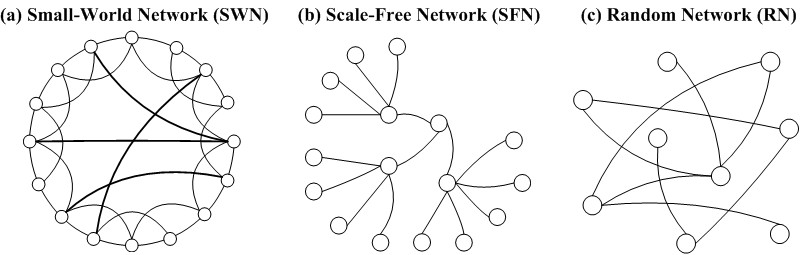
\includegraphics[width=6.3449in,height=2.0224in]{figures/chap3/chapitre3-img4.jpg}
    \caption{Types communs de réseaux}
\end{figure}

Les services de réseaux sociaux en ligne sont structurés en \textit{small-worlds}. Dans une étude analysant de larges corpus issus de différents services de réseaux sociaux en ligne, Kumar \& al. \citep{Kumar2006} ont montré que ces communautés possèdent toutes une structure et une évolution similaire. Les inscrits de chaque service se répartissent autour de trois grands groupes : \textit{singletons} (membres isolés, inactifs), \textit{giant component} (la majorité des utilisateurs actifs) et \textit{middle region} (des communautés isolées qui interagissent entre elles mais pas avec le reste du réseau). D{\textquoteright}après les auteurs, il existe très peu de chances que deux communautés isolées m\^eme très similaires se rencontrent dans ce type de réseau, car l{\textquoteright}entropie de la structure \textit{small-world }se renforce avec le temps en se fragmentant davantage. Une des raisons principales est que ces communautés isolées suivent souvent un modèle en \textit{étoile, }c{\textquoteright}est à dire qu{\textquoteright}elles sont construites autour d{\textquoteright}un individu central charismatique. éventuellement, il leur arrive de rejoindre la masse du \textit{giant component} mais elles en deviennent difficilement des acteurs majeurs et restent en périphérie. Dans un réseau social de type small-world comme les OSNS, les acteurs les plus influents sont ceux qui sont capables de 1) renforcer les liens dans un cluster (\textit{closure)} et 2) développer les connections faibles entre des clusters (\textit{brokerage)} (Burt, Centola, \& Kahl, 2008). Ce {\textquotedblleft}capital social{\textquotedblright} est inscrit dans la structure du réseau social lui-m\^eme \citep{Lin1999} et n{\textquoteright}a pas de relations avec le degré du node (son nombre de connections) \citep{Cha2010}. L{\textquoteright}individu le plus puissant d{\textquoteright}un réseau est donc celui possédant le plus grand nombre de connections \textit{potentielles, }proches et facilement accessibles et qui bénéficie d{\textquoteright}une place privilégiée pour bloquer ou autoriser l{\textquoteright}accès aux autres parties du réseau. L{\textquoteright}analyse organisationnelle a notamment montré l{\textquoteright}importance capitale des secrétaires pour le maintien d{\textquoteright}une bonne circulation des informations dans le réseau de l{\textquoteright}entreprise ou la nécessité d{\textquoteright}un nombre très faible de connections directes pour les acteurs importants de réseaux terroristes ou mafieux \citep{Russel2011}.


\subsection[Analyse de réseaux sociaux et de la diffusion d'information en ligne]{Analyse des réseaux sociaux et de la diffusion d'information en ligne}

L{\textquoteright}analyse de réseau social permet de comprendre la structure d{\textquoteright}un moment du réseau. En effet, les connections entre différents acteurs sont sans cesse en mouvement et l{\textquoteright}information en circulant vient modifier l{\textquoteright}activité du réseau et bien souvent sa structure m\^eme. Notre étude porte sur la diffusion de mèmes au sein du réseau social chinois Sina Weibo et s{\textquoteright}inscrit ainsi dans la continuité des travaux s{\textquoteright}intéressant aux rapports entre diffusion et technologies. Néanmoins, le champ de la diffusion de l{\textquoteright}innovation, objet traditionnel de la géographie, s{\textquoteright}est largement constitué autour des problématiques technologiques et organisationnelles liées à la situation spatiale du lieu et ses équipements \citep{Crevoisier2004}. Les études urbaines ont notamment montré comment la réalité économique et géographique présidait à la constitution des savoirs nécessaires à la diffusion de l{\textquoteright}innovation technologique \citep{Howells2002}. Cette vision doit \^etre modérée par une considération plus importante des modalités d{\textquoteright}appropriation des technologies comme pratiques propres aux territoires \citep{Fernandez2010}. Plus largement, les études sur la diffusion sont dominées par l{\textquoteright}analogie du virus comme modèle de propagation des messages, comportements et idées. Depuis la fin du XIXe siècle \citep{LeBon1895}, ce modèle est prépondérant dans les recherches autour de la diffusion d{\textquoteright}information en ligne \citep{Goel2012} Les membres de groupes dans un réseau seraient \textit{exposés }à un message ou une idée avant d{\textquoteright}\^etre \textit{infectés, }devenant alors porteur puis agent de sa diffusion. Ainsi, en considérant la position d{\textquoteright}un individu au sein du réseau de diffusion, il serait possible de définir un \textit{{\textquotedblleft}}\textit{degré d{\textquoteright}infection{\textquotedblright}} \citep{Cheng2013} et d{\textquoteright}anticiper la diffusion selon une \textit{{\guillemotleft}~probabilité immune~{\guillemotright} }qui\textit{ }déciderait de la \textit{{\guillemotleft}~qualité infectieuse~{\guillemotright} }de l{\textquoteright}objet diffusé ou de la \textit{{\guillemotleft}~possibilité de }\textit{rétablissement~{\guillemotright} }du sujet infecté \citep{Wang2011}. Cette analogie du viral propose une vision mécaniste qui fait peu de cas des facteurs contextuels ou psychologiques et ignorent ainsi les processus de décisions individuels en jeu \citep{Jackson2010}. Pourtant, nous savons notamment que le choix des mots ou la situation des personnes diffusant un message sont des facteurs décisifs et structurant des processus d{\textquoteright}adoption des messages en ligne \citep{Conover2013}.  En s{\textquoteright}intéressant à la diffusion géographique de mots dans les réseaux sociaux, Eisenstein \& al. \citep{Eisenstein2012} observe que leur diffusion se limite à un domaine géographiquement bien défini, dépendant de facteurs culturels et démographiques. Par exemple, les villes ayant d{\textquoteright}importantes communautés afro-américaines ont davantage de chances d{\textquoteright}adopter un m\^eme mot que d{\textquoteright}autres parfois plus proches géographiquement. Cette question est au centre des études de marketing qui s{\textquoteright}interrogent notamment sur l{\textquoteright}adoption de nouvelles marques ou de slogans. Afin de déterminer statistiquement les possibilités d{\textquoteright}adoption de produits et prévoir la pénétration dans un marché précis, la modélisation mathématique des effets de réseaux dans la diffusion est souvent utilisé \citep{Bass1994}. Ici, l{\textquoteright}analyse des données des réseaux sociaux est un grand enjeu pour la prospective économique et l{\textquoteright}application de ces modèles mathématiques aux données utilisateurs permettant de considérer des segments précis de marché. Le marketing politique fait lui aussi grand cas de l{\textquoteright}analyse de réseaux sociaux pour comprendre et orienter les discussions. La campagne de réélection d{\textquoteright}Obama aux USA en 2012 a fait un usage extensif de l{\textquoteright}analyse de données des réseaux sociaux pour identifier, déterminer et cibler des groupes sociaux particuliers gr\^ace au travail d{\textquoteright}une vaste équipe d{\textquoteright}ingénieurs et de \textit{{\textquotedblleft}data scientists{\textquotedblright}}\footnote{ \textit{{\textquotedblleft}Harper Reed, the chief technology officer for the Obama re-election campaign, who heads a team described as {\textquotedblleft}100 data scientists, developers, engineers, analysts, and old-school hackers [that] have been transforming the way politicians acquire data---and what they do with it.{\textquotedblright}, }from \ The Blaze \url{http://www.theblaze.com/stories/2012/10/03/very-creepy-details-of-obama-campaigns-voter-data-mining-effort/} consulté le 12 Mars 2014 à 14:50 GMT+1}. 

Une des grandes interrogations dans ce domaine est évidemment les r\^oles joués par les différents acteurs du processus de diffusion - et la manière de les identifier. Les études concernant les leaders d{\textquoteright}opinion, traditionnelles en sciences de la communication \citep{Katz1955} trouvent une continuité directe dans l{\textquoteright}étude des réseaux sociaux en ligne avec le domaine florissant des recherches sur l{\textquoteright}identification des \textit{influenceurs} \citep{Bakshy2011, Leavitt2009}. L{\textquoteright}analyse quantitative permet notamment de mieux comprendre l{\textquoteright}influence réelle des acteurs dans le réseau gr\^ace à l{\textquoteright}étude de leurs comportements. Le concept d{\textquoteright}influence sur les réseaux sociaux rev\^et en réalité des formes très variables et procède notamment d{\textquoteright}une légitimité construite autour de sujets précis par \ des personnes spécialisées devenues référentes \citep{Cha2010}. D{\textquoteright}autres {\textquotedblleft}influenceurs{\textquotedblright} possèdent une grande capacité d{\textquoteright}amplification pouvant par exemple initier le développement d{\textquoteright}une \textit{{\textquotedblleft}masse critique{\textquotedblright} }autour d{\textquoteright}une information\textit{, }définie classiquement comme le seuil d{\textquoteright}adoption à partir duquel la diffusion devient pérenne parmi une foule d{\textquoteright}acteurs \citep{Oliver2001}. L{\textquoteright}image quantitative d{\textquoteright}une {\textquotedblleft}masse{\textquotedblright} uniforme et actionnable dans le réseau est néanmoins remise en question par l{\textquoteright}étude de données dont l{\textquoteright}analyse montre que les relations entre différents acteurs du réseau sont à considérer qualitativement en termes de relations de pouvoirs \citep{Steyer2006}\textit{. }Les dynamiques d{\textquoteright}échanges ne répondent en effet pas tant à une relation pré-existente dans le réseau qu{\textquoteright}à un ensemble de situations o\`u les acteurs adoptent des comportements et des réactions particulières. La diffusion peut ainsi se comprendre comme une pratique du \textit{bouche-à-oreille} éminemment contextuelle, o\`u certains acteurs sont plus ou moins influents dans telle ou telle situation ou sur tel et tel sujet. Le temps joue néanmoins un r\^ole déterminant puisqu{\textquoteright}en considérant des séries de résultats o\`u des acteurs se c\^otoient durant plusieurs années, il est souvent difficile d{\textquoteright}identifier quel acteur influence l{\textquoteright}autre \citep{Aral2009}.

Après moins d{\textquoteright}un siècle d{\textquoteright}existence, l{\textquoteright}analyse de réseaux sociaux sous forme de graphes a donc connu une rapide évolution et une diversification dans de nombreux domaines de recherche. Les services de réseaux sociaux en ligne offrent notamment la possibilité d{\textquoteright}obtenir des données sur les comportements de groupes sociaux en très vaste quantité. Véritable vivier d{\textquoteright}études, ce champ de recherche en pleine expansion trouve ses origines dans des disciplines diverses qui poursuivent souvent des objectifs et des méthodes très différentes. Le tableau infra présente quelques-unes des méthodes d{\textquoteright}analyse de données définies selon leurs domaines d{\textquoteright}application. Ces méthodes coexistent souvent lors d{\textquoteright}études utilisant le \textit{data mining} ; nous présentons ici des exemples qui permettront ensuite de mieux situer nos perspectives de recherche~dans ce paysage de pratiques.

\begin{landscape}    
    \begin{spacing}{1} % line spacing

    \begin{ltabulary}{L| L J L J}
        &
        \textbf{Courant d{\textquoteright}analyse} &
        \textbf{Méthodologie} &
        \textbf{Exemples d{\textquoteright}usages et applications} &
        \textbf{Auteurs \& Publications de référence} \endhead
        
        \hline \\ [-0.5ex]

        1 &
        Graphes sociaux de groupe définis (cartographie de réseau fini) &
        En partant d{\textquoteright}un échantillon fini et déterminé au préalable, on effectue une carte des relations entre les différents acteurs du réseau.  &
        Cartographier les connections d{\textquoteright}après un profil sur un service de réseau social en ligne  &
        Cette pratique est l{\textquoteright}origine de la sociométrie (Moreno \& Jennings, 1938) et de l{\textquoteright}étude des relatons sociales en tant que réseaux.
        \\
        \hline \\ [-0.5ex]

        2 &
        Découverte de groupes par critères (communautés) &
        Cette méthode permet de réaliser un échantillonnage
        d{\textquoteright}un réseau social à partir d{\textquoteright}un
        ensemble de profils existants appelés \textit{seeds}. Un logiciel
        (appelé \textit{crawler}) va rechercher et collecter les profils
        similaires aux \textit{seeds} selon des critères définis :
        similarité, différence, profondeur, etc. &
        Identifier des communautés d{\textquoteright}après un type
        d{\textquoteright}utilisateur témoin

        Trouver des profils d{\textquoteright}utilisateurs similaires
        d{\textquoteright}après des profils existants &

        Hérité de la tradition de l{\textquoteright}échantillonnage
        \textit{{\textquotedblleft}boule de neige{\textquotedblright}} en
        statistiques \citep{Rothenberg1995}, les algorithmes de \textit{crawling}
        sont nombreux et il n{\textquoteright}existe pas de véritable
        consensus sur leur utilisation \citep{Gjoka2011}
        \\
        \hline \\ [-0.5ex]

        3 &
        Analyse sémantique des conversations (analyse de contenu)
         &
        En utilisant une masse textuelle de posts, un système est chargé
        d{\textquoteright}extraire et de classifier les mots et sujets
        discutés. Ce type de système se fonde sur l{\textquoteright}analyse
        naturelle de langage (NLP) et parfois sur l{\textquoteright}analyse
        structurelle des conversations \citep{Karandikar2010}.
         &
        Détection de tendances dans les conversations, Reconnaissance des
        entités dans un texte~(\textit{semantic tagging}) : noms de lieu,
        personnes, etc. &
        A mi-chemin entre linguistique et informatique \citep{Russel2011}, ce champ
        est un des grands enjeux actuels du Big Data \citep{Nettleton2013} avec
        notamment l{\textquoteright}analyse des sentiments (Liu \& Zhang, 2012)
        \\
        \hline \\ [-0.5ex]
        4 &
        Analyse de la diffusion 

        (évolution des \ relations d{\textquoteright}après une conversation)
        &
        D{\textquoteright}après une masse de posts extraites selon des
        critères précis (souvent un mot-clé ou \textit{hashtag}), il
        s{\textquoteright}agit ici de retracer les dynamiques relationnelles
        qui entourent ou suscitent la conversation en recréant le graphe
        social entourant la discussion et son évolution.  &
        Analyse d{\textquoteright}une campagne de marketing viral, Détection de communautés autour d{\textquoteright}un sujet précis, Détection d{\textquoteright}influenceurs \citep{Cha2010}

        R\^oles et partitionnement des acteurs de la diffusion \citep{Kwak2010b} &
        Le modèle classique du \textit{word-of-mouth }\citep{Steyer2006} et l{\textquoteright}approche
        épidémiologique \citep{Wang2011} sont souvent utilisés
        dans l{\textquoteright}analyse de la diffusion de contenus en ligne \citep{Cheng2013}.
        \\
        \hline \\ [-0.5ex]

        5 &
        Analyse comportementale et agents de diffusion (classifications et
        mesures)

        ~
         &
        Ici on étudie l{\textquoteright}activité d{\textquoteright}un ou
        plusieurs agents en analysant leur comportement dans le réseau
        (volume d{\textquoteright}activité, fréquence, etc.) souvent pour
        définir des critères et mesures qui permettent de classifier par
        type ou d{\textquoteright}anticiper les actions d{\textquoteright}un
        acteur du réseau. &
        Détection d{\textquoteright}influenceurs

        Mesures de la probabilité de diffusion \citep{Anagnostopoulos2012}

        Typologie des utilisateurs par comportement

        Effet psychologique des signaux sur un utilisateur &
        Présentes notamment dans le champ du marketing \citep{Leskovec2005} et de la politique \citep{Lotan2011}, 

        ce type d{\textquoteright}analyse cherche à comprendre et retracer les
        processus parfois psychologiques \citep{Robins2013} de prise de décisions
        individuelle.
        \\
        \hline \\ [-0.5ex]
        6 &
        Analyse contextuelle et géographique  &
        Ce type d{\textquoteright}analyse cherche à mettre en perspective des
        facteurs extérieurs au réseau afin d{\textquoteright}en comprendre
        l{\textquoteright}influence et les effets. Entre sciences sociales et
        informatique, ce type d{\textquoteright}étude porte souvent sur
        l{\textquoteright}usage du réseau plus que sur sa structure ou son
        évolution \citep{Torrens2010,Leetaru2013} &
        Approche sociologique des usages

        Mesures d{\textquoteright}impact \ géographique (node locality,
        geographic clustering coeficient) &
        L{\textquoteright}approche contextuelle dans l{\textquoteright}analyse
        de réseaux restent encore un champ à développer \ \citep{Adams2012}, notamment dans la considération de facteurs
        géographiques \citep{Graham1998, Onnela2011}, culturels \citep{Gallagher2013} ou de langage.
        \\
        \hline \\ [-0.5ex]
        7 &
        Simulation sociale &
        Afin de comprendre les dynamiques en l{\textquoteright}absence de
        données ou pour anticiper une situation à venir, il est possible de
        modéliser un environnement virtuel o\`u les comportements des acteurs
        sont simulés \citep{Macy2002}  &
        Prévision de tendances d{\textquoteright}après des données
        existantes

        Analyse de faits dont les données sont manquantes ou incomplètes &
        La découverte de méthodes de modélisation du contexte de
        l{\textquoteright}univers de simulation \citep{Ronald2012} est un des grands enjeux o\`u
        l{\textquoteright}apport de méthodes ethnographiques de terrain peut
        \^etre crucial \citep{Tubaro2010}\\
        
        % \caption[Tableau récapitulatif de méthodes d{\textquoteright}analyse de données de réseaux sociaux en ligne.]{Tableau récapitulatif de méthodes d{\textquoteright}analyse de données de réseaux sociaux en ligne.}
    \end{ltabulary}
    \end{spacing} % line spacing
\end{landscape}

Notre recherche choisit donc de s{\textquoteright}appuyer sur une étude de cas spécifique de Sina Weibo reprenant les éléments méthodologiques de l{\textquoteright}étude du graphe social de la diffusion entourant les conversations (Fig. 1-4) et l{\textquoteright}analyse sémantique des sujets dominants et sous-jacents aux conversations (Fig. 1-3). également, nous souhaitons amener une plus forte contextualisation des usages (Fig. 1-6) en prenant en compte notamment les relations entre les dimensions sémantique et conversationnelles, mais aussi géographique de l{\textquoteright}existence des conversations. L{\textquoteright}approche de l{\textquoteright}étude des données des SNS par les géographes notamment s{\textquoteright}est jusqu{\textquoteright}ici largement focalisée sur l{\textquoteright}analyse des \textit{geotag} et des cartes en ligne comme principale approche méthodologique \citep{Graham2011, Poorthuis2013}, réduisant considérablement les possibilités d{\textquoteright}étude des données de réseaux sociaux en ligne \citep{Crampton2013}. 


\subsection[Visualisation des échanges : les limites du modèle conversationnel]{Visualisation des échanges : les limites du modèle conversationnel}

L'analyse des échanges en ligne nécessite...

\begin{figure}[h!]
    \centering
    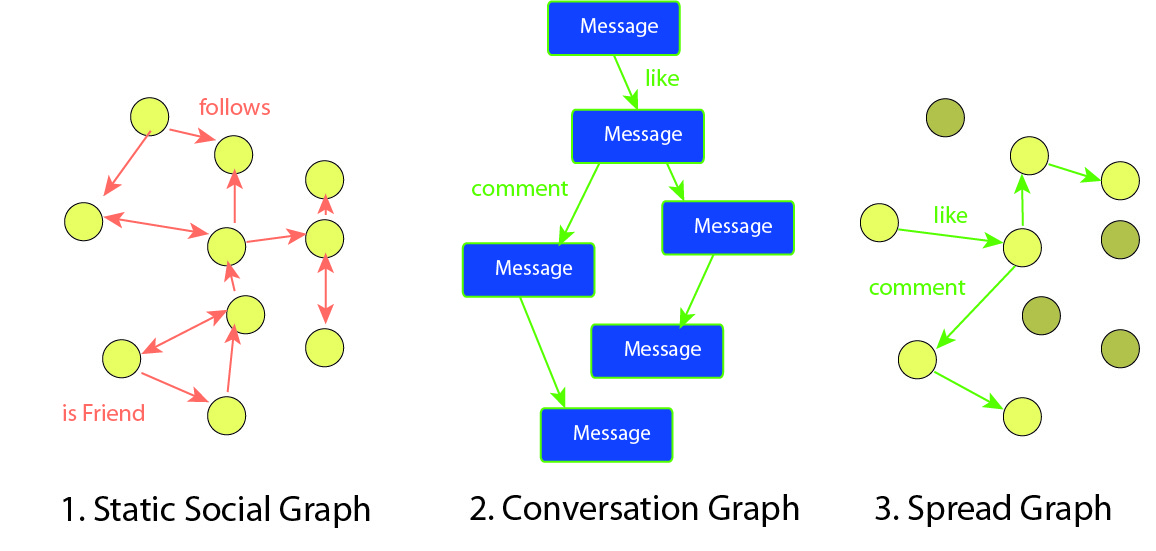
\includegraphics[width=6.2894in,height=3.0004in]{figures/chap3/chapitre3-img9.jpg}
    \caption[3 modèles de réseau]{Les 3 types de graphe classiquement extraits des données de réseaux sociaux}
\end{figure}

Plusieurs types de graphes peuvent \^etre extraits :

\begin{itemize}
\item \textbf{Graphe social statique}: représentant les relations pré-existantes dans la structure du réseau étudié (untel est ami avec untel, untel suit untel, etc.)
\item \textbf{Graphe conversationnel}: représentant toutes les interactions qui entourent et structurent la diffusion de messages 
\item \textbf{Graphe de diffusion}: représentant les interactions qui se sont produites entre les acteurs durant \ la diffusion du message. Ce dernier type de graphe est un recoupement des deux autres.
\end{itemize}


Dans notre étude, le graphe social statique ne présente pas particulièrement d{\textquoteright}intér\^et puisqu{\textquoteright}il correspond à un ensemble de relations peu affecté par les discussions. De plus, nous ne disposons dans le jeu de données Weiboscope que de son état final qui ne témoigne pas de l{\textquoteright}évolution des relations. Nous voulons obtenir ici les graphes de diffusion sous la forme de conversations structurées\textbf{~(}graphe directionnelle des \ réponses et commentaires) de l{\textquoteright}ensemble des messages. Dans un article paru dans \textit{Nature} \citep{Weng2012}, les chercheurs du \textit{Centre de Recherche sur les Systèmes Complexes} de l{\textquoteright}Université d{\textquoteright}Indiana identifient les caractéristiques des mèmes connaissant le plus de succès (la plus large diffusion). Un travail de visualisation de mèmes identifiés par des hashtags sur Twitter leur permet notamment de mettre à jour des motifs particuliers dans la structure des conversations.


\begin{figure}[ht]
    \centering
    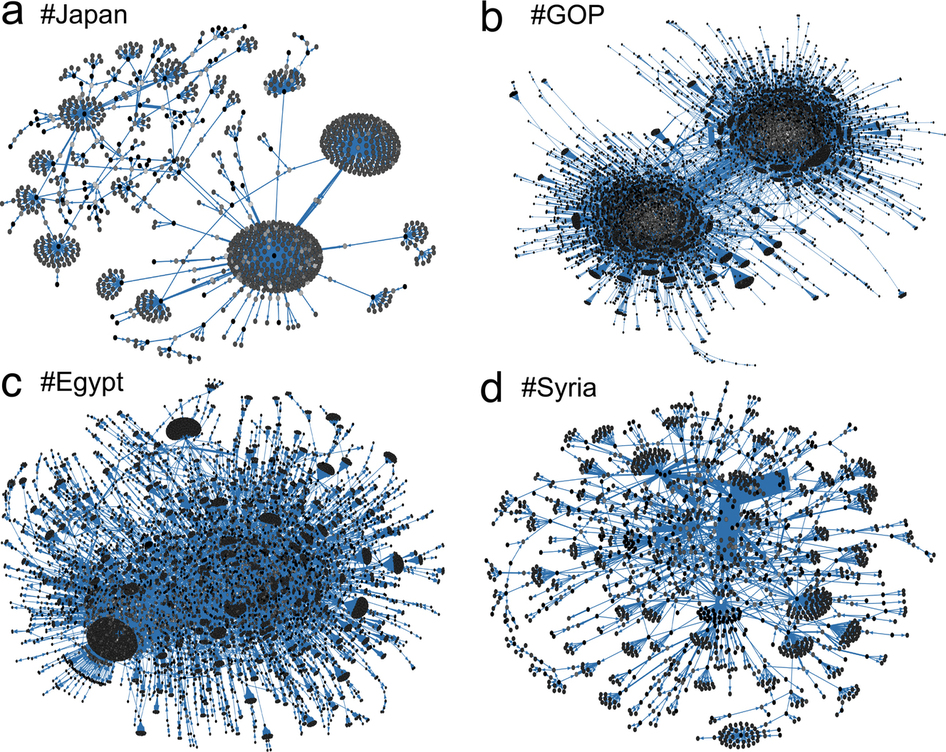
\includegraphics[width=5.5669in,height=4.4224in]{figures/chap3/chapitre3-img10.jpg}

    Nodes represent Twitter users, and directed edges represent retweeted posts that carry the meme. The brightness of a node indicates the activity (number of retweets) of a user, and the weight of an edge reflects the number of retweets between two users. \newline
    (a) The \textit{\#Japan}  meme shows how news about the March 2011 earthquake propagated. \newline
    (b) The \textit{\#GOP} tag stands for the US Republican Party and as many political memes, displays a strong polarization between people with opposing views. \newline
    Memes related to the Arab Spring and in particular the 2011 uprisings in (c) \textit{\#Egypt} and (d) \textit{\#Syria} display characteristic hub users and strong connections, respectively.
    
    \caption{Graphe de diffusion de hashtags sur Twitter d{\textquoteright}après \citep{Weng2012} }

\end{figure}


Nous avons mené un travail préliminaire afin de mener plusieurs expérimentations sur la visualisation de graphes conversationnels. Après avoir identifié quelques-uns des hashtags les plus discutés de l{\textquoteright}année 2012 sur Sina Weibo (voir la section \ref{sec:hashtags}), nous avons procédé à la visualisation des échanges pour chacun d'entre eux. Afin de mettre à jour le graphe conversationnel entourant les hashtags sélectionnés sur Sina Weibo, nous avons choisi d{\textquoteright}extraire la séquence d{\textquoteright}interactions des messages (mentions, retweets) composant chaque mème (voir algorithme \ref{algo:hashtags-graph}.

\begin{figure}
    
    \label{algo:hashtags-graph}
    % Hashtags
    \begin{algorithm}[H]
        \caption{Hashtags conversational graphs}
        \begin{algorithmic}
            \Require{$M$ is a set of microblog messages}
            \State $H(h,Gh)$ is a set of all hashtags conversational graphs

            \Function{HashtagsGraph}{$M$}
                \For{message $m$ in $M$}

                    \If{hashtag $h$ in $m$} 
                        \State $Gh=(Vh,Eh)$ is $h$ conversational graph
                        \If{ quotes or rt $e(userA,userB)$ in $m$}
                            \State $Eh \gets e(userA,userB)$ and $Vh \gets userA,userB $
                        \EndIf
                        \State $H \gets (h,Gh)$ 
                    \EndIf
                \EndFor
            \EndFunction
        \end{algorithmic}
    \end{algorithm}
    \caption{Algorithme pour constituer les graphes conversationnels des hashtags d'après un ensemble de message}
\end{figure}

Cette structure de graphe nous permet de représenter la diffusion de chaque mème sous forme d{\textquoteright}un graphe contenant un node par utilisateur et un ensemble de relations correspondant aux échanges visibles dans les textes des messages. Dans un premier temps, le logiciel \textit{Graphviz }nous a permis d{\textquoteright}obtenir une représentation basique du graphe conversationnel afin d{\textquoteright}avoir un aper\c{c}u sur la nature des conversations par l{\textquoteright}observation des motifs qui la compose. En effet, si les deux mesures identifiées à l{\textquoteright}étape précédente (volume de messages et \ volume d{\textquoteright}échanges) nous permettent d{\textquoteright}effectuer un premier tri parmi les hashtags, cette première visualisation nous permet de considérer la nature des échanges et l{\textquoteright}implication des utilisateurs d{\textquoteright}après la structure des motifs conversationnels. Chaque utilisateur est symbolisé par un point et chaque message par un trait reliant deux utilisateurs. Un motif très compact reflète une conversation animée entre des utilisateurs peu nombreux échangeant beaucoup. A l{\textquoteright}inverse, un motif disparate reflète des échanges plus brefs et morcelés.

\begin{figure}[ht]
    
    \begin{minipage}[b]{0.4\linewidth}
        \centering
        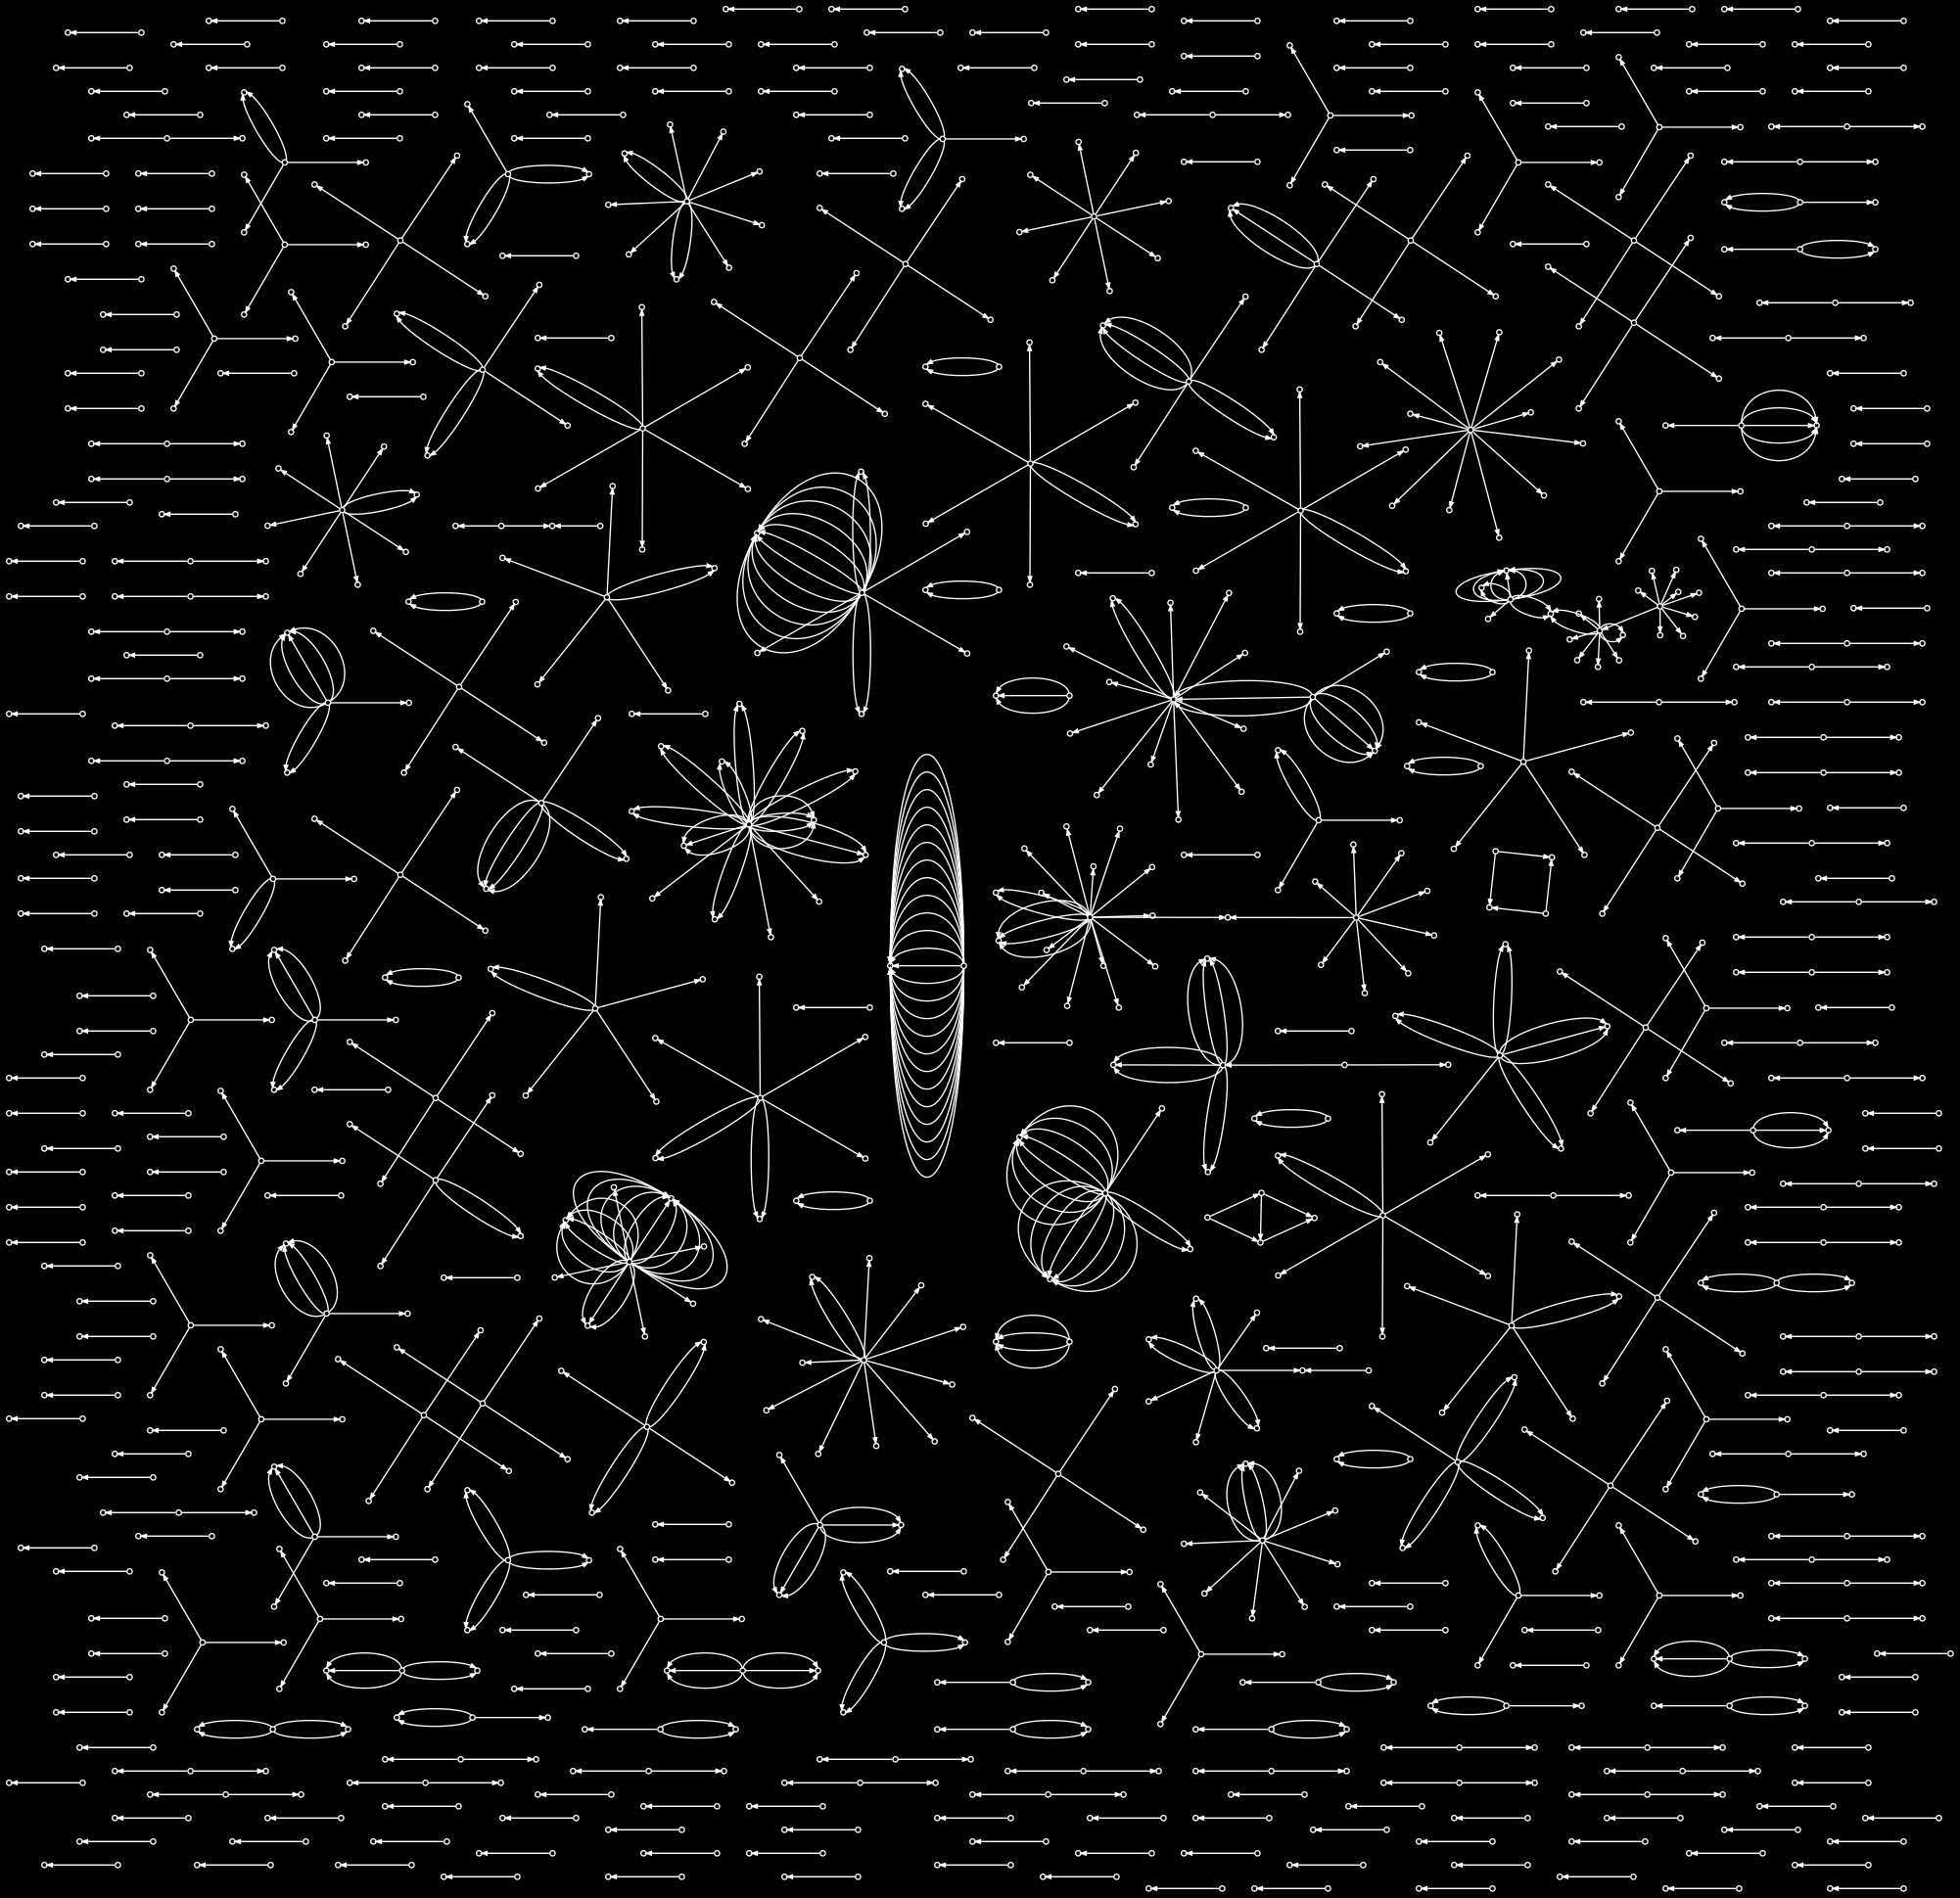
\includegraphics[width=2.5in,height=2.5in]{figures/chap3/chapitre3-img11.png}
        \par\vspace{0pt}
    \end{minipage}
    \begin{minipage}[b]{0.55\linewidth}
        \centering
        \raggedright
        \textit{WeicoPlus }est une application mobile permettant
        d{\textquoteright}utiliser Sina Weibo. Le hashtag \#WeicoPlus\# est
        ajouté automatiquement quand les utilisateurs postent des photos
        depuis ce service. 

        Ainsi, on remarque que le graphe conversationnel
        entourant WeicoPlus se compose essentiellement de messages simples,
        mais ne donne pas lieu à une conversation structurée - à
        l{\textquoteright}exception de quelques rapides échanges entre un
        nombre réduit de personnes.
        \par\vspace{0pt}
    \end{minipage}

    \caption[Visualisation simple du hashtag{\textquotedblleft}WeicoPlus{\textquotedblright}] {Fig. Visualisation simple du hashtag{\textquotedblleft}WeicoPlus{\textquotedblright}, un trait représente un échange entre deux utilisateurs}
\end{figure}


\begin{figure}[ht]
    \begin{minipage}[b]{0.4\linewidth}
        \centering
        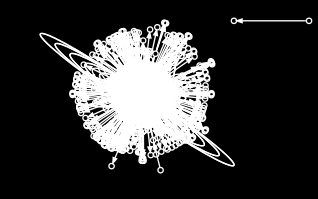
\includegraphics[width=2.5in,height=1.5in]{figures/chap3/chapitre3-img12.png}
        \par\vspace{0pt}
    \end{minipage}
    \begin{minipage}[b]{0.55\linewidth}
        \centering
        \raggedright
        A l{\textquoteright}inverse, le hashtag {\textquotedblleft}Veuve
        d{\textquoteright}enfant
        unique{\textquotedblright} \zh{\#失独母亲\#} cristallise
        le débat en une forme très dense qui reflète une surenchère de
        commentaires et d{\textquoteright}actions autour du hashtag, propre
        d{\textquoteright}une conversation animée. 
        \par\vspace{0pt}
    \end{minipage}

    \caption[Visualisation simple des conversations autour du hashtag Veuve d{\textquoteright}enfant unique]{Visualisation simple des conversations autour du hashtag Veuve d{\textquoteright}enfant unique}
\end{figure}

Les différents modèles de conversation que nous obtenons dans cette première étape se présentent sous une forme schématique et peu détaillée. Afin de comprendre plus en détails les dynamiques conversationnelles qui les entourent, nous avons choisi de sélectionner trois exemples parlants de hashtags dont les graphes conversationnels présentent des particularités des modèles de diffusion dissemblables et organisés. Pour chacun d{\textquoteright}eux, nous allons procéder à une analyse plus détaillée des graphes conversationnels afin de considérer les différences entre ces différents modèles.

% \begin{figure}[th]
%     \centering
%     \subfloat[Pluie torrentielle à Tianjing]{
%         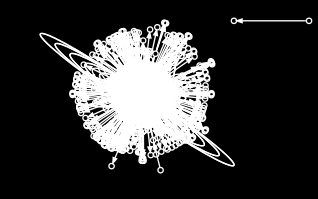
\includegraphics[width=2.3224in,height=1.4449in]{figures/chap3/chapitre3-img13.png}
%     }

%     \subfloat[Veuve à l{\textquoteright}enfant unique]{
%         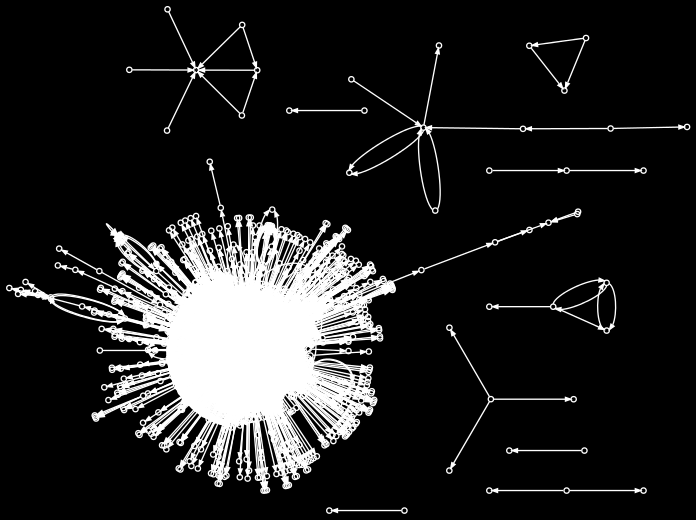
\includegraphics[width=2.3004in,height=1.7224in]{figures/chap3/chapitre3-img14.png}
%     }

%     \subfloat[Abolition des lois sur la prostitution]{
%         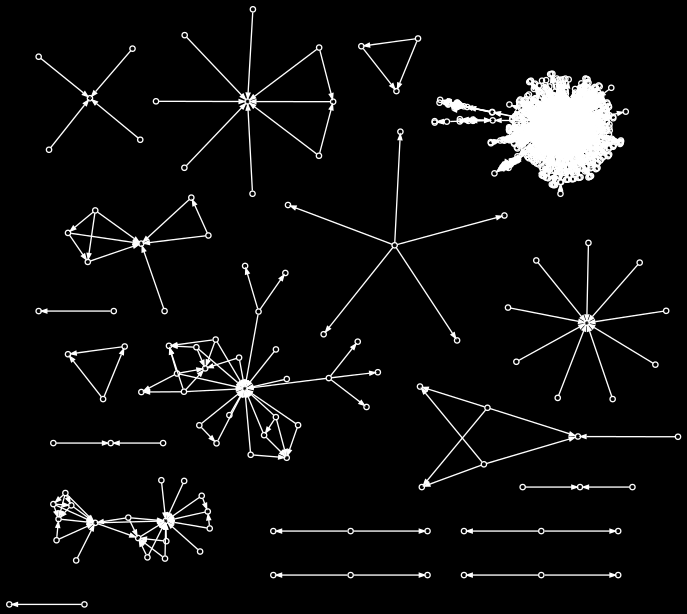
\includegraphics[width=2.1449in,height=1.9224in]{figures/chap3/chapitre3-img15.png}   
%     }
  
%     \caption{Visualisation des conversations autour de trois hashtags}
% \end{figure}


Nous voyons que les trois représentations des graphes ci-dessus donnent à voir des structures plus ou moins morcelées, avec un ensemble de points et de lignes très compactes qui représentent la majeure partie de la conversation. Afin de visualiser plus précisément les groupes et les dynamiques qui constituent les discussions autour de chaque hashtag, nous allons utiliser le logiciel Gephi \citep{Bastian2009} afin d{\textquoteright}examiner de plus près la composition de ces graphes. Pour ce faire, Gephi va nous permettre d{\textquoteright} {\textquotedblleft}étaler{\textquotedblright} le graphe en repositionnant les nodes et en les coloriant pour en identifier les composantes et les tendances.

Chaque utilisateur est représenté sous la forme d{\textquoteright}un point. La taille des points correspond à l{\textquoteright}importance de l{\textquoteright}utilisateur dans le réseau total des échanges, caractérisé par son degré de centralité intermédiaire (\textit{betweenness centrality}), une mesure topologique correspondant au nombre de plus courts chemins du graphe passant par cet utilisateur. La couleur est utilisée pour représenter la \textit{modularité }du réseau, c{\textquoteright}est à dire le nombre de communautés engagées dans la conversation définies comme les cliques d{\textquoteright}utilisateurs constituant plus de 1\% du réseau total d{\textquoteright}échange \citep{Blondel2008}. La position des nodes est calculée gr\^ace à l{\textquoteright}algorithme \textit{Force Atlas 2} \citep{Bastian2009} utilisant une modélisation physique o\`u les nodes peu connectés entre eux se repoussent et ceux très connectés s{\textquoteright}attirent. Ainsi, la proximité de deux nodes sur le graphe témoigne d{\textquoteright}une proximité lors des conversations, c{\textquoteright}est à dire de l{\textquoteright}existence d{\textquoteright}un échange entre eux (citations, commentaires ou retweets). Pour davantage de visibilité, certaines conversations sub-alternes représentant moins de 1\% du total ont été effacées. Egalement, les nodes possédant un degré inférieur à 3 (moins d{\textquoteright}un échange avec au moins trois autres nodes du grahe) ne sont pas représentés.

\textbf{Exemple 1 : Pluie torrentielle à Tianjing}

Le premier mème choisi parle d{\textquoteright}une catastrophe naturelle, sous la forme d{\textquoteright}une pluie diluvienne qui s{\textquoteright}est abattue sur la ville de Tianjin durant la nuit du 21 au 22 Juillet 2012.

\begin{figure}[h!]
    \centering
    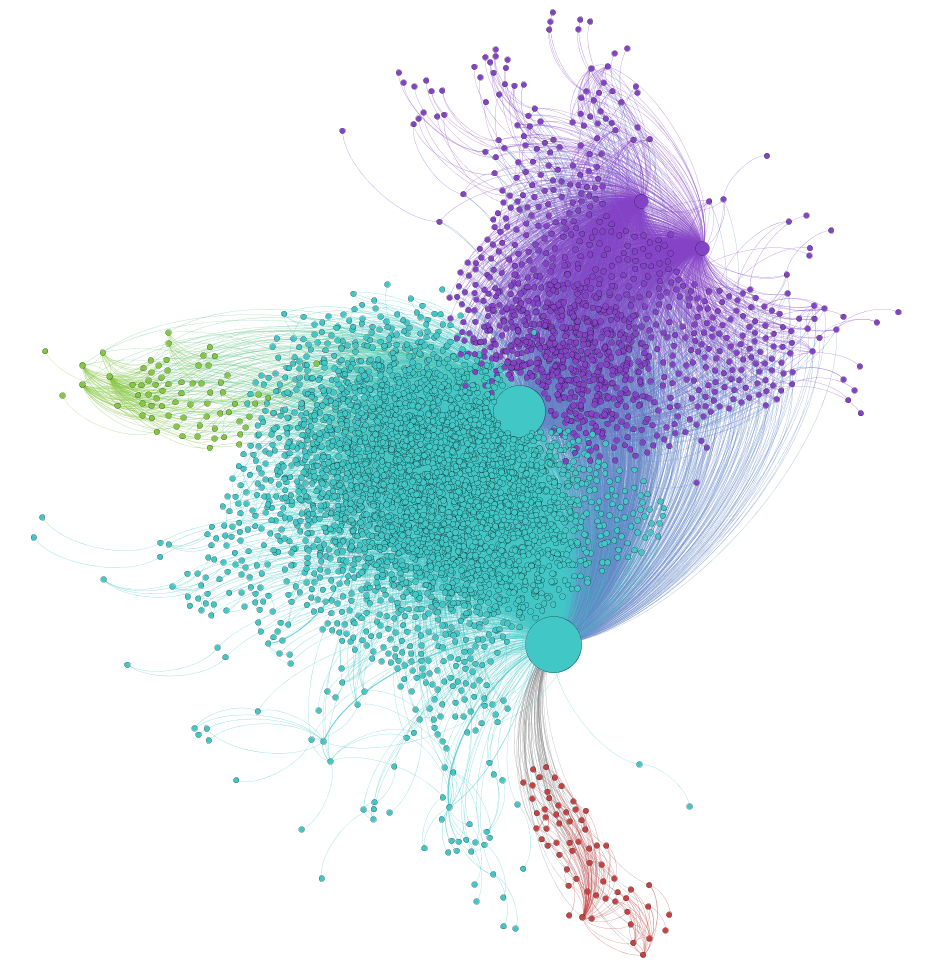
\includegraphics[width=6in,height=6in]{figures/chap3/chapitre3-img17.png}
    \caption{Exemple 1 : Tianjin Baoyu}
    \label{fig:graph-tianjin}
\end{figure}

Sur la figure \ref{fig:graph-tianjin}, on voit nettement 4 groupes constitués autour de gros diffuseurs (les nodes les plus gros) qui composent 85\% du graphe. Plusieurs groupes semblent s{\textquoteright}emparer de la conversation mais on voit peu d{\textquoteright}activité entre les nodes alors que les échanges se déroulent autour de quelques utilisateurs très centraux. Cela traduit le fait que peu de personnes ont réellement discuté l{\textquoteright}information et elles se sont simplement contentées de la relayer.


La diffusion d{\textquoteright}un fait divers très local (il se passe à Tianjing) est entrainée par peu de sources très importantes (les quelques nodes de grande taille), vraisemblablement des journaux et médias locaux qui annoncent la nouvelle (presse, photos-choc d{\textquoteright}innondations, etc). La conversation est peu active et très structurée, nous sommes en présence d{\textquoteright}un modèle classique de diffusion de masse.

\begin{figure}[h!]
    \centering
    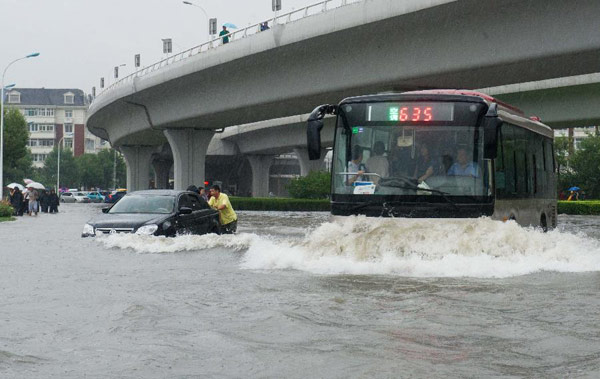
\includegraphics[width=4.76in,height=3in]{figures/chap3/chapitre3-img16.jpg}
    \caption[Photo de Tianjin durant la pluie torentielle en Juillet 2012]{\textit{Downpour bypasses Beijing, batters neighbor, }in Qinghua News le 2012-07-26 13:29:59, \url{http://news.xinhuanet.com/english/china/2012-07/26/c_131740415.htm} consulté le 27 Juin 2014.}
\end{figure}

\textbf{Exemple 2 : Veuve de l{\textquoteright}enfant unique}

Un autre sujet discuté par une très large quantité de personnes appara\^it sous le terme {\textquotedbl}\textit{shidu muqin}{\textquotedbl}, forme contractée signifiant \textit{{\textquotedblleft}mère qui a perdu son enfant unique{\textquotedblright}} (\zh{\#失独母亲\#}). Ce hashtag désigne un phénomène de société bien connu en Chine o\`u le deuil de la perte d{\textquoteright}un enfant se double souvent pour une mère chinoise seule de l{\textquoteright}absence de ressources pour vivre. En effet, l{\textquoteright}absence de système de retraite fait porter aux enfants la responsabilité de la survie de la famille.

\begin{figure}[h!]
    \centering
    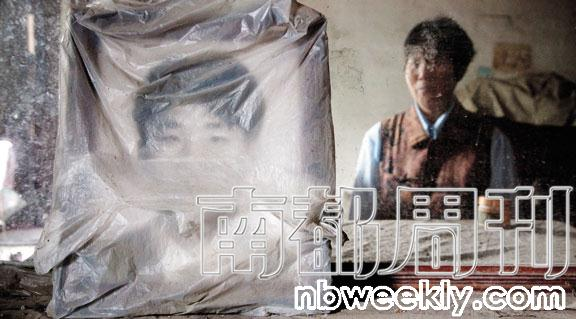
\includegraphics[scale=0.7]{figures/chap3/chapitre3-shidumuqin.jpg}
    \caption[Photo illustrative de Shidu Muqin]{\zh{一位失独母亲的独语} paru le 17 Juillet 2012 in \textit{Nandu Weekly} le 2012.07.17, \url{http://www.nbweekly.com/news/special/201207/30571.aspx}, consulté le 27 Juin 2014.}
    \label{fig:photo-shidumuqin}
\end{figure}


\newpage


Le graphe \ref{fig:shidumuqin} ici est fait de deux grands groupes composant à eux deux près de 95\% du graphe total. Les discussions sont très polarisées et menées par peu de participants (les nodes les plus gros sur le graphe). Peu de personnes très influentes concentrent les discussions autour d{\textquoteright}eux, accompagnés ou suivis d{\textquoteright}une foule de commentateurs.  

\begin{figure}[h!]
    \centering
    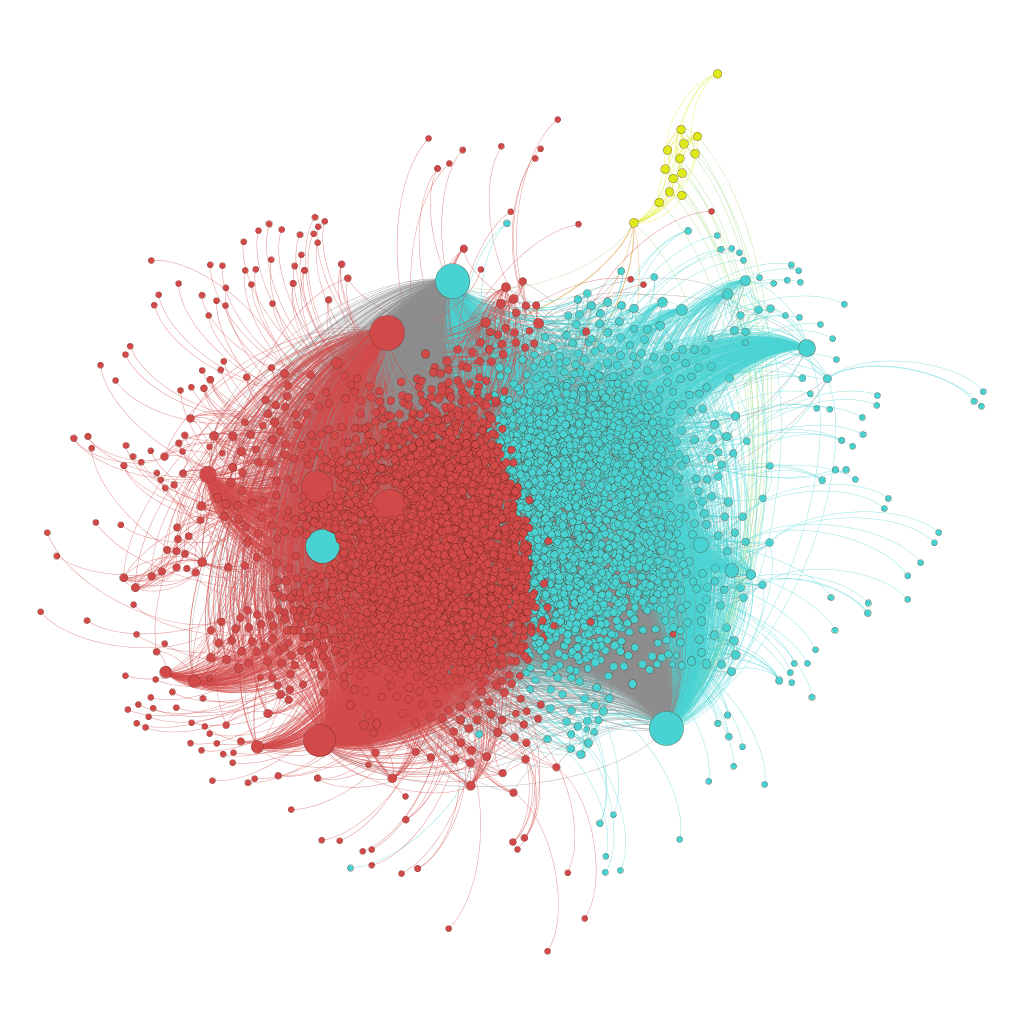
\includegraphics[width=6.0114in,height=6.0114in]{figures/chap3/chapitre3-img18.png}
    \caption{{\textquotedblleft}Shidu Muqin{\textquotedblright}}
    \label{fig:shidumuqin}
\end{figure}



Cet exemple donne à voir des groupes bien définis et très proches o\`u plusieurs acteurs majeurs mènent la discussion. Les dynamiques d{\textquoteright}échanges autour d{\textquoteright}une question de société (la loi de l{\textquoteright}enfant unique en Chine et ses conséquences) s{\textquoteright}articule en groupes distincts sans pour autant amener à des controverses importantes (qui se traduiraient par des discussions longues et houleuses). Ici, les leaders d{\textquoteright}opinion font la discussion et la diffusion se fait au travers d{\textquoteright}eux.

\clearpage
\textbf{Exemple 3 : Abolition des lois sur la prostitution}

Le hashtag \textit{{\textquotedblleft}Abolissons la loi piaowudong nuzui{\textquotedblright} }est l{\textquoteright}expression d{\textquoteright}une campagne pour l{\textquoteright}abolition d{\textquoteright}une législation scandaleuse sur la prostitution en Chine. Depuis les années 80, la loi chinoise interdit la prostitution et prévoit la condamnation des deux parties qui s{\textquoteright}adonnent à un échange d{\textquoteright}argent. Baptisé \textit{{\textquotedblleft}Piaowudong nuzui{\textquotedblright}, }cette loi a vu plusieurs cas absurdes impliquant des viols organisés sur mineurs se solder par la condamnation et l{\textquoteright}emprisonnement des enfants incriminés. Relayés par les journalistes, les scandales à répétition ont éclatés à plusieurs reprises, impliquant parfois des officiels du Parti souvent blanchis alors que des enfants étaient eux emprisonnés. 

\begin{figure}[th]
    \centering
    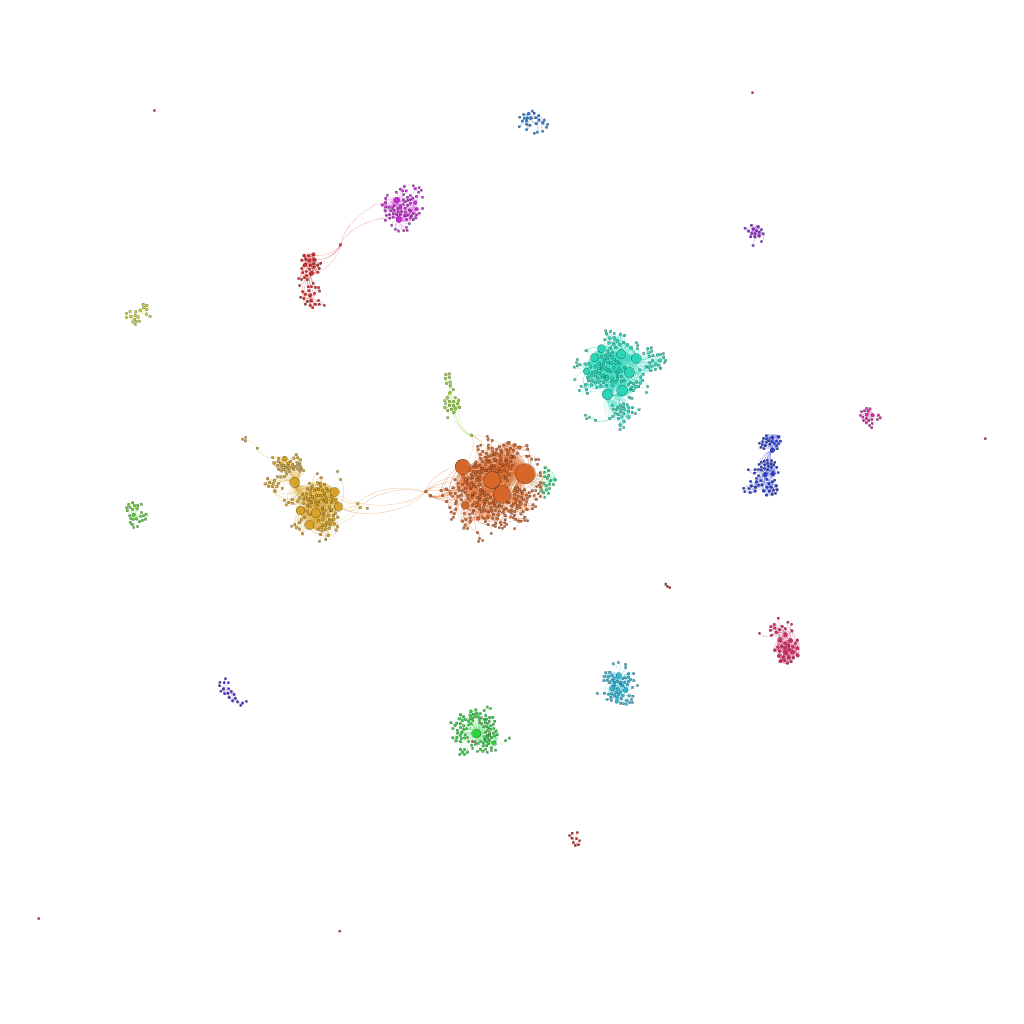
\includegraphics[width=6.0114in,height=6.0114in]{figures/chap3/chapitre3-img19.png}
    \caption{ {\textquotedblleft}Piaowudong nuzui{\textquotedblright}}
    \label{fig:piaodong}
\end{figure}

Le graphe \ref{fig:piaodong} des discussions autour de l{\textquoteright}abolition de cette loi montre que de nombreux groupes discutent séparément de cette question puisque les premiers 50\% du graphe sont déjà constitués de plus d{\textquoteright}une quinzaine de clusters. Les groupes sont très éloignés entre eux, n{\textquoteright}entretenant que peu de relations et connaissant une activité intense.


Cet exemple présente les caractéristiques d{\textquoteright}une conversation très décentralisée dans laquelle de nombreux acteurs différents prennent part. L{\textquoteright}émergence de ce type de discussion fragmentée témoigne d{\textquoteright}un usage particulier de la discussion sur le réseau social et montre comment la discussion autour d{\textquoteright}un sujet peut s{\textquoteright}étendre sans afficher de relations directes dans le média lui-m\^eme. Ici un agent extérieur (en l{\textquoteright}occurence un article du journal \textit{Nanfang Zhoumo }sur le sujet) fait na\^itre la conversation sans pour autant l{\textquoteright}accaparer et la centraliser. Plus difficilement détectable et contr\^olable, cette dernière configuration est typique du mème car elle se développe de fa\c{c}on large et durable entre des groupes à l{\textquoteright}origine peu connectés.


\bigskip

Cette première visualisation des graphes conversationnels nous permet d{\textquoteright}explorer quelques types précis d{\textquoteright}échanges et d{\textquoteright}en proposer une première lecture. Néanmoins, le procédé de visualisation reste rudimentaire et soulève plusieurs questions que nous nous donnons pour t\^ache de continuer à explorer. Premièrement, dans quel espace a lieu cette représentation? En étalant ainsi ces graphes conversationnels, quelle action réalisons-nous réellement et quelle en est la valeur pour l{\textquoteright}analyse? à plus forte raison, quelle est la relation de cette espace du graphe conversationnel avec les autres formes d{\textquoteright}espace, et plus notamment l{\textquoteright}espace du réel géographique et l{\textquoteright}espace de la représentation par le langage?

Nous souhaitons ici mettre en perspective ces différentes dimensions afin d{\textquoteright}enrichir le modèle d{\textquoteright}étude. En effet l{\textquoteright}analyse de la diffusion utilise principalement les graphes des réseaux de diffusion mettant en scène les utilisateurs et leurs interactions en ligne. Loin d{\textquoteright}\^etre inintéressant, ce type de schéma est néanmoins très réducteur car il se fonde sur un modèle communicationel très primaire \textit{{\textquotedblleft}émetteur-récepteur{\textquotedblright} }dont on conna\^it les limites. Les travaux de Jacobson ont notamment permis d{\textquoteright}étoffer ce modèle en considérant les différents aspects fonctionels des actes de communication.


\begin{figure}[h!]
    \centering

    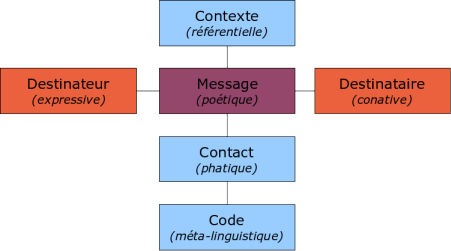
\includegraphics[width=4.6894in,height=2.6114in]{figures/chap3/chapitre3-img5.png}

    \caption[Modèle de Jakobson]{ Le modèle de Jakobson présente différents aspects des actes de communication que nous pouvons chercher à adapter dans le contexte des échanges en ligne.}

\end{figure}

Ainsi, en nous basant sur les modèles des théories de la communication, nous pouvons peut-\^etre améliorer les modèles méthodologiques d{\textquoteright}analyse. Nous proposons ici la notion de \textit{topogramme }comme modèle pour comprendre les motifs de diffusion des mèmes, considérés comme \textit{topos} ou \textit{lieux communs. }Le topogramme, en tant que représentation graphique des différentes dimensions et dynamiques lisibles dans les données nous permet donc d{\textquoteright}approcher un travail \ d{\textquoteright}observation précise de la diffusion des mèmes, voire par la suite de classification des actes de communication en ligne. Afin de prendre en compte, les différents aspects de la communication, il nous faut donc effectuer une analyse à plusieurs niveaux (multi-layers), regroupant un ensemble de réseaux à la fois sémantique, conversationnel et géographique.      % épistémo et méthodo
\section{Méthodes d'identification de mèmes dans un large volume de donneés}
\label{sec:id-meme}

Choisir un ensemble de mèmes cohérents est une des étapes difficiles de notre recherche. En effet, dans parmi les millions de messages de notre corpus et plus généralement dans la multitude des échanges quotidiens sur les réseaux sociaux, trouver une prise pour l{\textquoteright}étude n{\textquoteright}est pas une t\^ache évidente. Cette section présente les résultats obtenus lors de différentes expérimentations pour constituer des corpus de données représentatifs de mèmes dans un large volume de données.

\subsection[Constitution et collection d{\textquoteright}un corpus de messages]{Constitution et collection d{\textquoteright}un corpus de messages}
\label{sec:weiboscope}

La plupart des services de réseaux sociaux en ligne offrent un large accès à leur données. En effet, il s{\textquoteright}agit souvent de la fondation de leurs modèles d{\textquoteright}affaires basés sur la valorisation et la revente de ces données pour le marketing ciblé \citep{Ko2010}. Pour entrer en contact avec la base de données, les SNS mettent à disposition une API (\textit{Application Programming Interface}) qui permet à un programme ou une autre application web de se connecter au service pour demander et obtenir des données. L{\textquoteright}API est donc la première source d{\textquoteright}obtention de données depuis les SNS. Néanmoins, les données des réseaux sociaux sont soumises à d{\textquoteright}importants enjeux et contraintes tant commerciales, éthiques que politiques - dans le cas de la Chine notamment. Les conditions d{\textquoteright}utilisations techniques et légales (\textit{Terms of Uses) }de ces données sont également soumises à des changements fréquents, étroitement liés à l{\textquoteright}évolution commerciale et technologique de compagnies souvent très jeunes. Nous avons établi une liste des limitations et écueils pouvant \^etre rencontrés lors de l{\textquoteright}extraction et de l{\textquoteright}analyse de données des SNS :

\begin{description}
    
    \item[Compatibilité] 
    \hfill \\
    Une solution technologique devient facilement caduque lors de l{\textquoteright}évolution d{\textquoteright}une API (ex. la version  v1.0 de l'API de \textit{Twitter } n{\textquoteright}existe plus, ainsi le code doit \^etre réécrit pour la version 1.1).  
    
    \item [Disponibilité] 
    \hfill \\
    Chaque API répond à des formats et critères précis et possède ses propres limitations. Pour accéder à l{\textquoteright}API du moteur de recherche de Sina Weibo, il faut s{\textquoteright}identifier auprès de la compagnie gr\^ace à une carte d{\textquoteright}identité et des paiements par requ\^ete sont exigés.

    \item[Limitations d{\textquoteright}usage] 
    \hfill \\
    Afin de limiter le trafic et conserver le contr\^ole sur les données distribuées, les SNS mettent en place des limitations d{\textquoteright}accès à leurs serveurs, notamment : limitation du nombre de requ\^etes par heure, limitation du nombre de requ\^etes par machine (basée sur l{\textquoteright}adresse IP), limitation du nombre d{\textquoteright}utilisateurs connectés. Ainsi, Twitter limite à 150 requ\^etes API par heure pour un compte non-identifié, pouvant augmenter jusqu{\textquoteright}à 500 après authentification. Les données datant de plus de 7 jours sont payantes, reflétant la valeur d{\textquoteright}un accès en {\textquotedblleft}temps-réel{\textquotedblright} aux données.
    
    \item[Légalité]
    \hfill \\
    Les données sont soumises aux conditions de propriété décrites légalement par la firme qui les publient \citep{Clifton2006}. Ces conditions sont susceptibles de changer. Ainsi, Twitter a exigé en 2012 le retrait a posteriori de nombreux jeux de données publiés par des chercheurs depuis plusieurs années parfois \citep{McCreadie2012}. Actuellement, Twitter précise notamment dans ses \textit{Terms of Use: {\textquotedblleft}You may not resyndicate or share Twitter content, including datasets of Tweet text and follow relationships{\textquotedblright} }\footnote{ Terms of use de Twitter, \url{https://dev.twitter.com/terms/api-terms}, consulté le 12 Mars 2013 à 17h08}.
    
    \item[Ethique]
    \hfill \\
    Vous pouvez extraire depuis une API des profils d{\textquoteright}utilisateurs contenant les informations qu{\textquoteright}ils ont auparavant publié en ligne \citep{Felt2008}. En exposant les données personnelles des utilisateurs, le chercheur est responsable de l{\textquoteright}usage qu{\textquoteright}il en fait, pouvant notamment exposer des utilisateurs \citep{Rieder2005}.  
\end{description}

Afin d{\textquoteright}obtenir des données et de contourner les limitations de l{\textquoteright}API, la pratique dite du \textit{{\textquotedblleft}scraping{\textquotedblright} }permet d{\textquoteright}obtenir des données à l{\textquoteright}aide d{\textquoteright}un robot qui lit et sauvegarde des parties ou l{\textquoteright}intégralité de pages web. Les moteurs de recherche utilisent notamment cette technique pour l{\textquoteright}indexation des pages. Ce type de pratiques est également soumis à des limitations par les services web (blocage de l{\textquoteright}IP source) et se situe à la limite de la légalité,voire est explicitement interdit dans le cas de certains SNS \citep{Petschulat2010}.

Un programme appelé \textit{spider }ou \textit{crawler} est chargé d{\textquoteright}effectuer des requ\^etes régulières à l{\textquoteright}API afin d{\textquoteright}obtenir et collecter les informations obtenues dans une base de données. Plusieurs approches existent dans les techniques d'échantillonnage de réseau social. La première, fondée sur des mots-clés extraits les posts contenant des mots ou des hashtags particuliers. La seconde utilise l{\textquoteright}échantillonnage de graphe, collectant au fil des liens les conversations ou profils des utilisateurs. Classique des études statistiques, cet échantillonage dit \textit{boule de neige {\textquotedblleft}élargit l{\textquoteright}échantillon en partant d{\textquoteright}un node original pour s{\textquoteright}éloigner vers ses voisins{\textquotedblright}} \citep{Rothenberg1995}. Ici, deux grandes catégories s{\textquoteright}opposent : les techniques traversales o\`u les nodes sont classifiés après avoir été visités et les {\textquotedblleft}walk{\textquotedblright} aléatoires o\`u l{\textquoteright}extension du graphe visité se fait de manière aléatoire \citep{Gjoka2011}.

Au cours du travail préparatoire de cette recherche, nous avons tout d{\textquoteright}abord expérimenté plusieurs algorithmes et outils de collection de données afin d{\textquoteright}en comparer les résultats. Une première approche d{\textquoteright}extraction par utilisateurs a été infructueuse car la sélection du groupe source (\textit{seeds}) ne permettait pas d{\textquoteright}obtenir des résultats cohérents\footnote{Code disponible : \url{https://github.com/sharismlab/Pyweibo}, consulté le 14 Mars à 5h32}. Par la suite, une autre approche de collecte de données via le développement d{\textquoteright}un plug-in pour le navigateur Google Chrome\footnote{Code disponible : \url{https://github.com/sharismlab/battlefield}, consulté le 14 Mars à 5h12} nous a permis de tester et d{\textquoteright}apercevoir les limites de la collection de données par mots-clés. Cette étape nous a également montré l{\textquoteright}intér\^et que peut présenter une approche collaborative de la collection de données ou de seeds par un système collaboratif de {\textquotedblleft}curation{\textquotedblright} afin d{\textquoteright}obtenir des éléments précis de contenus et de réduire la masse de données inutiles qui pollue souvent les jeux de données \citep{Ding2013}. Après de multiples tests et comparaisons d{\textquoteright}outils et de librairies, plusieurs difficultés majeures limitaient l{\textquoteright}obtention d{\textquoteright}une quantité de données suffisantes, notamment la nécessité de ressources assez importantes (en terme de développement et de disponibilité des machines), un temps d{\textquoteright}acquisition parfois très long et l{\textquoteright}exigence d{\textquoteright}une veille constante sur les SNS pour identifier un mème au bon moment (les tweets de Sina Weibo devenant indisponibles via l{\textquoteright}API au-delà de 7 jours). La première limite se situe bien s\^ur dans la capacité d{\textquoteright}une personne seule à mener à bien cette large t\^ache. Nous avons donc choisi de considérer les jeux de données collectés sur Sina Weibo disponibles sur l{\textquoteright}Internet. Une fois écartés les nombreux jeux tronqués, modifiés ou incomplets, nous avons pu obtenir plusieurs jeux de données provenant de recherches préalables dans le domaine particulier de l{\textquoteright}échantillonnage \citep{Ding2013} ou ayant servi de bases à des études précédentes \citep{Gao2012}. Finalement, nous avons identifié le jeu de données constitué lors du projet \textit{Weiboscope }de l{\textquoteright}Université de Hong Kong comme répondant à nos besoins en termes de dimensions (temps, nombre d{\textquoteright}utilisateurs observés), taille (nombre de tweets) et contenus (géo-localisation, présence des tweets censurés).


Notre travail d{\textquoteright}analyse s{\textquoteright}appuie donc sur ce jeu de données collecté sur le service de microblog Sina Weibo par le \textit{Journalism and Media Studies Centre} (JMSC) de l{\textquoteright}Université de Hong Kong lors de son projet \textit{Weiboscope}. Téléchargeable ouvertement, la publication de ce jeu de données a pour objectif de \textit{{\textquotedblleft}enables academic use of the data for better understanding of the social }\textit{media in China and making the Chinese media system more transparent.{\textquotedblright}}\footnote{Le jeu de données Weiboscope est disponible à l{\textquoteright}adresse : \url{http://147.8.142.179/datazip/}, consulté le 14 Mars à 17h21}\textit{ }Il s{\textquoteright}agit d{\textquoteright}un échantillonnage aléatoire de messages \textit{(random sampling)} effectué quotidiennement durant toute l{\textquoteright}année 2012 sur un panel d{\textquoteright}environ 350 000 utilisateurs ayant au moins 1000 followers \citep{Fu2013}. La totalité du jeu de données comprend 226,841,122 messages répartis sur 52 semaines, dont des messages ayant été supprimés par les utilisateurs eux-m\^emes ou par les administrateurs de Sina Weibo eux-m\^emes - parfois sur ordre du gouvernement chinois (\textit{ibid}, 2013).

\begin{table}[ht]
    \centering
    \small
    \begin{tabulary}{\textwidth}{c|C} 
        \toprule
        \textbf{Désignation}
        & \textbf{Description} \\
        \hline \\[-1.5ex]

        mid  &
        Unique pseudo message ID\\[2ex]
        retweeted\_status\_mid  &
        Pseudo message ID of the original message (Only available if the row of
        interest is a retweet)\\[2ex]
        Uid &
        Pseudo user ID\\[2ex]
        retweeted\_uid &
        Pseudo user ID of the original poster (Only available if the row of
        interest is a retweet)\\[2ex]
        Source &
        The application name of the client program\\[2ex]
        Image &
        With image? (1= Yes, 0=No)\\[2ex]
        text  &
        body of the message. Any address handle (@xxxx:) is replaced by either
        the pseudo user ID or ukn (uknown)\\[2ex]
        geo &
        GIS information. Please refer to the Sina Weibo API documentation:
        \url{http://goo.gl/Um8SS}\\[2ex]
        created\_at &
        Original posting time\\[2ex]
        deleted\_last\_seen &
        The last seen time before this message was missing from the user
        timeline\\[2ex]
        permission\_denied  &
        {\textquotesingle}permission denied{\textquotesingle} status is marked
        when the message was found missing in the timeline and the API return
        message was {\textquotesingle}permission denied{\textquotesingle} - See
        details in (Fu, Chan, Chau 2013)\\[2ex]
    \end{tabulary}
    \caption[Modèle de messages pour le jeu de données Weiboscope]{Modèle de messages pour le jeu de données Weiboscope}
\end{table}

Ce jeu de données a été mis à disposition sous une forme anonymisée o\`u les identifiants des messages et des utilisateurs ont été remplacés par des pseudo-identifiants. La collection des données a été effectuée sur une série d{\textquoteright}utilisateurs (génération aléatoire d{\textquoteright}identifiants dont l{\textquoteright}existence est ensuite validée) pour donner \textit{{\textquotedblleft}une image représentative des usages et utilisateurs de Sina Weibo (...) dont les études auparavant limitée à des analyses non-aléatoire (...) se cantonnaient aux utilisateurs les plus populaires{\textquotedblright} }\citep{Fu2013}.Cet échantillon s{\textquoteright}attache à refléter les pratiques des utilisateurs {\textquotedblleft}lambda{\textquotedblright}. Ce jeu de données a déjà été partiellement étudié dans le but de comprendre la démographie des utilisateurs de Sina Weibo, leurs activités et les comportements pouvant permettre de prédire les réactions notamment de censure. La démographie des utilisateurs se composent de 55\% d{\textquoteright}hommes habitant principalement dans les grandes villes de Chine (Pékin, Canton, Shanghai). Une des découvertes importantes est le très faible taux de création originale de messages malgré une activité importante des utilisateurs, indiquant que l{\textquoteright}essentiel de l{\textquoteright}activité sur Sina Weibo se constitue de re-posts et de commentaires \citep{Fu2013}. Le jeu de données est accompagné des informations succintes de profil des utilisateurs dont le lieu, rempli par eux, sans néanmoins fournir leurs noms d{\textquoteright}utilisateur véritables. Notre travail de recherche s{\textquoteright}articule autour d{\textquoteright}une nouvelle lecture de ce jeu de données unique.

\subsection[Détection algorithmique de mèmes]{Détection algorithmique de mèmes dans un large corpus de données}
\label{sec:protomemes}

Une fois l{\textquoteright}acquisition des données effectuée, il s{\textquoteright}agit désormais de savoir les analyser correctement pour y déceler les mèmes que nous souhaitons observer. Les travaux dans le domaine de la détection et l{\textquoteright}identification de mèmes dans les données de réseaux sociaux restent encore peu nombreux. Une des études pionnières est l{\textquoteright}outil \textit{MemeTracker }(devenu \textit{NIFTY}) con\c{c}u en 2009 par le \textit{SNA Project }de l{\textquoteright}Université de Stanford \citep{Leskovec2009}. Cet outil permet une étude sous forme de graphes de la diffusion de phrases dans un vaste corpus de texte mais n{\textquoteright}est pas adapté à la langue chinoise. La discussion sur la modélisation mathématiques des mèmes \citep{Ahmad2006, Nye2011} émane souvent de recherches en informatique cherchant à prendre en considération différents facteurs de diffusion lors de l{\textquoteright}analyse machine de données \citep{Zubiaga2011, Wang2011}, considérant parfois le mème comme un vecteur de modification du réseau lui-m\^eme \citep{Ienco2010}. Plus marginal, des études s{\textquoteright}intéressent aux dynamiques géographiques des mèmes \citep{Kamath2013}. Néanmoins, aucune de ces différentes approches ne permet d{\textquoteright}apporter une réponse technologique ou algorithmique satisfaisante pour l{\textquoteright}identification de mèmes Internet dans un ensemble de données issu des réseaux sociaux. Afin de déceler les mèmes dans un vaste ensemble textuel, nous devons y déceler des motifs de diffusion particuliers. La dénomination \textit{machine learning }regroupe un ensemble d{\textquoteright}algorithmes qui permettent d{\textquoteright}explorer des jeux de données pour en extraire des représentations et y identifier des propriétés (\textit{features}) particulières. Basé sur les sciences statistiques, ces algorithmes font usage de mesures de similarité pour classifier les éléments d{\textquoteright}un corpus. Les catégories utilisées pour la classification peuvent \^etre définies au préalable par l{\textquoteright}utilisateur - c{\textquoteright}est le \textit{{\textquotedblleft}supervised learning{\textquotedblright} }ou inférées du jeu de données lui-m\^eme dans le cas du \textit{{\textquotedblleft}unsupervised learning{\textquotedblright}}\citep{Breiman2001}. La multitude d{\textquoteright}algorithmes de \textit{machine learning }disponibles pour la détection de \textit{clusters} au sein d{\textquoteright}un corpus textuel ou d{\textquoteright}un réseau social \citep{Nettleton2013, Robins2013} rend l{\textquoteright}identification d{\textquoteright}une solution difficile. De plus, les algorithmes utilisés traditionnellement pour l{\textquoteright}analyse de documents textuels (\textit{topic modeling, LSA}) se heurtent au caractère très disparate des corpus issus des réseaux sociaux (\textit{text sparsity issue) }faisant diminuer drastiquement leur efficacité \citep{Hong2010}.

\cite{Ferrara2013} propose dans un papier intitulé {\textquotedblleft}\textit{Meme clustering in social media}{\textquotedblright} un algorithme utilisant la classification automatique non-supervisée pour détecter des mèmes dans un corpus de données de réseaux sociaux. Ce travail récent propose de tenir compte non seulement des textes et hashtags, mais aussi des liens et des modèles de diffusion pour identifier des groupes de messages intéressants et procéder au \textit{clustering }des mèmes. L{\textquoteright}algorithme s{\textquoteright}articule autour du concept de {\textquotedblleft}protomèmes{\textquotedblright}, représentant les éléments fondamentaux d{\textquoteright}un mème en cours de création \citep{Gabora1995}. Dans le contexte des médias sociaux, le protomème est défini par les entités (liens, hashtags...), mots-clés et séquences de conversation qui constitue le mème en devenir. En identifiant puis comparant les différents protomèmes présents dans chaque tweet, il est possible d{\textquoteright}y détecter des similarités et de deviner les mèmes en formation.  

\begin{figure}[htbp]
    \centering
    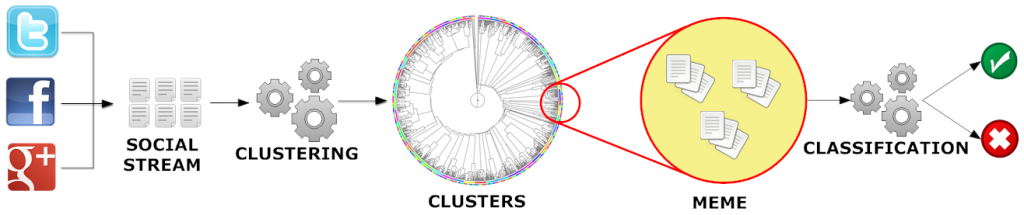
\includegraphics[width=5.8894in,height=1.2114in]{figures/chap3/chapitre3-img6.png}
    \caption{Algorithme de reconnaissance de mème (clustering) \citep{Ferrara2013}}
\end{figure}

Cet algorithme suppose donc d{\textquoteright}extraire dans un premier temps les éléments remarquables du corpus de tweets afin d{\textquoteright}établir des représentations de ces protomèmes contenant les éléments à comparer : \textit{phrases} (texte brut), \textit{mentions }(@, RT), \textit{hashtags} et \textit{urls}. Pour constituer ces jeux de protomèmes, nous utilisons le pattern \textit{map-reduce} qui permet de chercher et lister des éléments dans un vaste jeu de données \textit{(map)} avant de les regrouper dans une liste \textit{(reduce)}. Une fois ces protomèmes constitués, nous procédons à leurs comparaisons selon plusieurs critères :

\begin{itemize}
\item \textit{Similarité de texte }: comparant le contenu texuel de chaque protomème 
\item \textit{Similarité d{\textquoteright}utilisateurs} : comparant les utilisateurs contenus dans chaque protomème
\item \textit{Similarités de tweet }: recherchant les tweets identiques dans différents protomèmes
\item \textit{Similarité de diffusion : }considérant les références aux utilisateurs contenus dans chaque protomème
\end{itemize}

Ici nous utilisons la \textit{sémantique vectorielle} (Support Vector Machine) afin de comparer les éléments des protomèmes gr\^ace à une représentation algébrique sous formes de vecteurs. Pratique ancienne de l{\textquoteright}algèbre linéaire appliquée à la science informatique \citep{Salton1975}, il s{\textquoteright}agit de permettre la conversion d{\textquoteright}objets textuels (mots, identifiants, images...) sous une forme aisément comparable. Pour convertir le texte sous forme vectorielle, l{\textquoteright}algorithme classique Tf-idf (\textit{Term Frequency - Inverse Document Frequency}) est utilisé \citep{Soucy2005}. Les autres mesures de similarité sont la \textit{mesure cosine (}ou \textit{similarité cosinus) }des protomèmes convertis sous forme de vecteurs binaires. Une fois ces différentes valeurs de similarité calculées, nous utilisons les scalaires définis dans le papier de référence pour assigner des poids à chacun des vecteurs et les combiner en une seule valeur \citep{Ferrara2013}. Cette matrice de valeurs de similarité nous permet alors de définir les protomèmes les plus similaires et d{\textquoteright}identifier ainsi des \textit{clusters }dans les données correspondant aux mèmes.


Si cette approche offre des résultats probants sur de petits volumes (quelques centaines de tweets), la très grande demande en puissance de calcul et ressources mémoires nécessaires rendent le traitement d{\textquoteright}un jeu données plus vaste irréalisable. Les opérations de comparaison et le calcul de similarités sur de vastes volumes de données font cro\^itre très rapidement la complexité des algorithmes et ainsi la quantité de calculs à effectuer. Le calcul du co\^ut d{\textquoteright}un algorithme se fait au travers des notions dites de domination, avec notamment le {\textquotedblleft}grand O{\textquotedblright} exprimé \textit{O(f(n)) }qui fait correspondre à la complexité d{\textquoteright}un algorithme une fonction \textit{f} de la quantité d{\textquoteright}information manipulée \textit{n. }Ainsi pour un algorithme courant de complexité \textit{O(n}\textit{\textsuperscript{2}}\textit{), }les ressources de calcul \textit{(computation)} et de mémoire (RAM ou stockage) nécessaires augmentent de manière exponentielle à chaque élément ajouté au corpus \textit{n}. L{\textquoteright}algorithme de {\textquotedblleft}meme clustering{\textquotedblright} décrit par Ferrara atteint donc un co\^ut exorbitant devant un large volume de données comme celui du jeu Weibosope. La limite physique de calcul est rapidement atteinte rendant impossible le franchissement du pallier expérimental et la vérification des hypothèses de travail à une échelle suffisante. Ainsi, nous allons poursuivre ces expérimentations en nous intéressant désormais aux hashtags.

\subsection[Les hashtags ne sont pas des mèmes]{Les hashtags ne sont pas des mèmes}
\label{sec:hashtags}

Les \textit{hashtags }(en fran\c{c}ais {\textquotedblleft}mots-dièses{\textquotedblright}) sont utilisés dans l{\textquoteright}écriture sur les réseaux sociaux et se présentent dans Sina Weibo sous la forme d{\textquoteright}un mot entouré de deux dièses - ex. \textit{\#mot-clé\#}. Marqueur particulier, le hashtag permet à un interlocuteur de procéder à une dénotation ou connotation du message original \citep{Romero2011} ou d{\textquoteright}affirmer son caractère évènementiel (lors d{\textquoteright}un évènement sportif, d{\textquoteright}une conférence, etc). Facile à identifier dans la masse des données en ligne, il permet de désigner un ensemble de contenus sous un m\^eme signe. Ainsi, il est un vecteur important permettant de collecter simplement une large masse d{\textquoteright}informations autour d{\textquoteright}un mème. La constitution d{\textquoteright}un corpus autour d{\textquoteright}un {\textquotedblleft}hashtag{\textquotedblright} présente néanmoins plusieurs limites. Premièrement, le mème est par définition un objet en mutation. Ainsi, il est souvent difficile de l{\textquoteright}identifier une bonne fois pour toute par un ou plusieurs de mot-clés. De plus, le mème existe bien souvent sous la forme d{\textquoteright}images ou de vidéos qui ne sont pas nécessairement légendées ou référencées et donc peu accessible à une recherche {\textquotedblleft}plein texte{\textquotedblright}. Ainsi, une approche pour la recherche de mèmes ne peut \^etre entièrement textuelle et doit s{\textquoteright}intéresser aux autres forme de contenus web (notamment les liens). De plus, l{\textquoteright}ajout de hashtags dans les messages est un acte volontaire non systématique. Ainsi, si l{\textquoteright}identification de certains mèmes peut se faire gr\^ace à la recherche de hashtags, l{\textquoteright}ensemble des messages contenant des hashtags ne recouvrent pas systématiquement un mème. Comme nous le verrons, les hashtags sont bien souvent de simples artefacts de campagne marketing en ligne.

Afin de procéder à l{\textquoteright}analyse des mèmes, nous avons donc indexé l{\textquoteright}ensemble des contenus du corpus Weiboscope contenant des hashtags sur toute l{\textquoteright}année 2012 (30 millions sur un total de 200 millions tweets environs). Nous avons donc dans un premier temps extrait l{\textquoteright}ensemble des messages contenant un ou des hashtags de l{\textquoteright}ensemble des données avant de les classifier pour obtenir des jeux de données cohérents par hashtags. L{\textquoteright}extraction des hashtags est effectuée gr\^ace à une expression régulière qui scanne le texte pour identifier et préserver uniquement les caractères situés entre les deux signes dièse (\#).


% Process Hashtags
\begin{figure}[htpb]
    \begin{algorithm}[H]
        \caption{Extract Hashtags from Message}
        \label{algo:message-graph}
        \begin{algorithmic}

            \Require{$m$ is a microblog text message}

            \Function{ExtractEntities}{$m$}
                
                \If{begins with \# and ends with \#}
                    \State $h\gets hashtag$
                    \State $text\gets u$ from 
                    % \State $H\gets->$h$
                \EndIf

            \EndFunction
        \end{algorithmic}
    \end{algorithm}
    \caption[Algorithme d'extraction d'entités d'après les messages]{
        \textit{Algorithme d'extraction d'entités d'après les messages}
        Les entités extraites des messages sont : les hashtags, les citations et les mots importants.

    }
\end{figure}

Sur un total d{\textquoteright}environ 30 millions de tweets contenant des hashtags, nous avons choisi de retenir seulement les hashtags possédant plus de 1000 messages et d{\textquoteright}ignorer les 1000 hashtags les plus utilisés. En effet, ils ne présentaient pas d{\textquoteright}intér\^et pour notre étude, étant la plupart du temps des noms de marque ou des mots-clés trop généraux (par exemple : {\textquotedblleft}bonne nuit{\textquotedblright}, {\textquotedblleft}nouvelles de sports{\textquotedblright}, {\textquotedblleft}photos de nourriture{\textquotedblright}, etc).

\begin{figure}[htpb]
    \centering
    
    \begin{tabular}{c|c|c|c}
        \textit{hashtags} & \textit{users} &  \textit{actions} & \textit{tweets} \\
        \hline\\ [-1ex]
        \zh{吴奇隆} & 201 & 13243 & 22349  \\
        \zh{一起到老} & 182 & 0 & 364  \\
        \zh{春运} & 92 & 13 & 256  \\
        \zh{轻松一刻} & 92 & 11 & 240  \\
        \zh{人品值分析} & 90 & 490 & 321  \\
        \zh{朝阳区} & 88 & 49 & 165  \\
        \zh{理性态小度} & 87 & 0 & 329  \\
        \zh{美图GIF} & 87 & 101 & 404  \\
        \zh{我正在听} & 86 & 6 & 330  \\
        \zh{微盘签到} & 84 & 304 & 305  \\
        \zh{2012来了} & 83 & 206 & 309  \\
        \zh{中级达人} & 83 & 0 & 159  \\
        \zh{分享} & 82 & 87 & 563  \\
        \zh{星座} & 82 & 5 & 195  \\
    \end{tabular}

    \caption[Hashtags les plus utilisés pendant la 1ère semaine de 2012]{\textit{Hashtags les plus utilisés pendant la 1ère semaine de 2012} - Les résultats concernant la 1ère semaine de l{\textquoteright}année 2012 donnent un aper\c{c}u du volume analysé : 5,044,331 tweets, 398 392 utilisateurs uniques cités (dans un total de 2 115 544 mentions), 264 651 urls uniques (pour un total de 426 914) et 44 382 hashtags uniques (pour un total de 244285).}
\end{figure}


Notre étude vise à analyser les dynamiques conversationnelles et nous devons donc déterminer les plus adéquats parmi des hashtags de nature souvent très différentes. Pour ce faire, nous avons sélectionné pour chaque jeu de données (chaque hashtag) deux mesures significatives : premièrement, le volume de messages ; deuxièmement, la quantité d{\textquoteright}échanges et d{\textquoteright}interactions effectives entre les utilisateurs (commentaires, retweets, etc.). Ces deux mesures nous permettent de nous assurer que 1) nous possédons une quantité suffisante de messages pour mener à bien l{\textquoteright}étude et que 2) la discussion a bien eu lieu et qu{\textquoteright}il ne s{\textquoteright}agit pas de messages redondants ou non reliés entre eux. Nous avons choisi d{\textquoteright}ignorer les échanges dominés à plus de 80\% par le m\^eme utilisateur pour éviter la pollution de l{\textquoteright}étude par l{\textquoteright}activité de robots. Le graphe ci-dessous permet d{\textquoteright}observer la distribution de 429 hashtags possédant tous plus de 1000 tweets et 1000 échanges : l{\textquoteright}axe vertical représente la quantité d{\textquoteright}actions (échanges) et l{\textquoteright}axe horizontal le volume des conversations. Tout en bas du graphe se trouvent donc les hashtags ayant été les moins discutés, avec en haut ceux aux conversations les plus intenses. La taille des points illustre le volume de messages et la couleur la quantité de conversations.
% je ne comprends pas le code couleur % 

\begin{figure}[htpb]
    \centering
    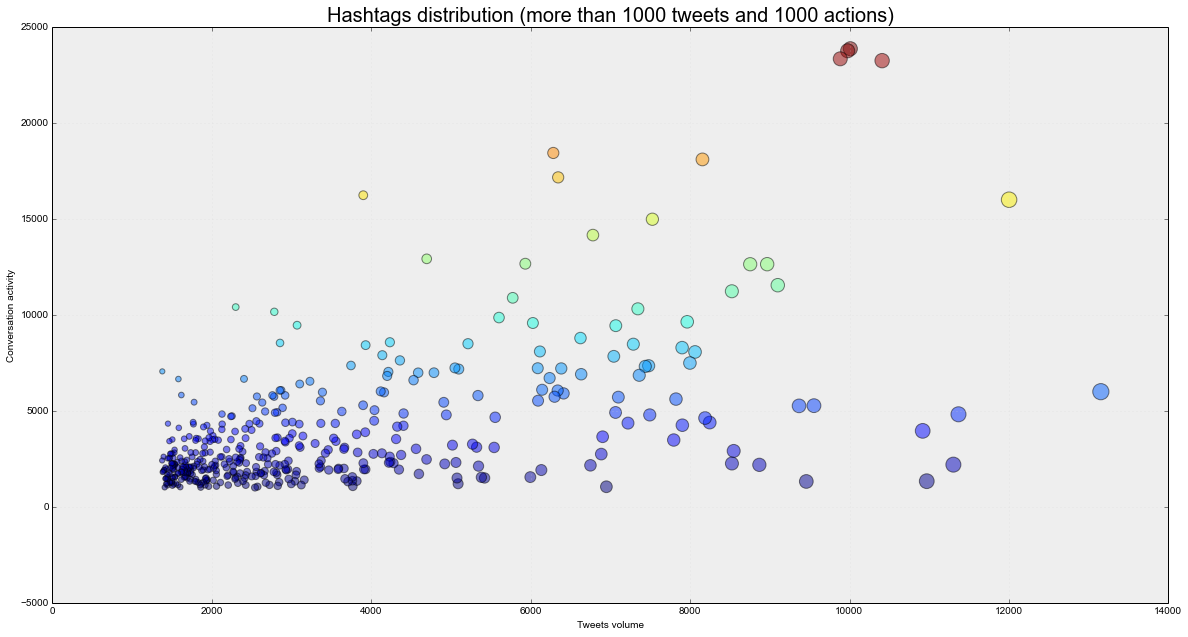
\includegraphics[width=6.0114in,height=3.2114in]{figures/chap3/chapitre3-img8.png}
    \caption{Distribution des 429 hashtags les plus discutés}
\end{figure}


En procédant à l{\textquoteright}étiquetage des hashtags les plus actifs durant l{\textquoteright}année 2012 sur Sina Weibo (figure 2 ci-dessus), nous constatons que la plupart sont associés à des activités commerciales, de loisirs ou de divertissement. Ici nous observons que les usages majoritaires du réseau social Sina Weibo correspondent pour la plupart à ceux d{\textquoteright}autres mass-médias plus traditionnels de par le monde. Le commerce en ligne occupe notamment une place proéminente. La marque de téléphonie mobile chinoise \textit{Xiaomi} est abondamment citée, reflétant son importance croissante dans le marché chinois et surtout sa stratégie commerciale qui cible abondamment les réseaux sociaux avec de nombreux hashtags très discutés (notamment \textit{{\textquotedblleft}Fans de Xiaomi{\textquotedblright} } \#\zh{小米粉丝}\# ). Également, de nombreuses campagnes promotionnelles d{\textquoteright}ouverture ou d{\textquoteright}anniversaire de magasins ont réussi à se hisser dans le jeu de t\^ete des hashtags les plus discutés. Radio-crochets ou chanteurs reconnus, les stars de la télévision et de la chanson sont aussi présents dans le peloton de t\^etes des discussions sur Sina Weibo. Le célèbre chanteur Han Geng notamment compte près d{\textquoteright}une dizaine de hashtags le concernant parmi les 500 les plus discutés (\textit{{\textquotedblleft}Han Geng fait une pub pour Nokia{\textquotedblright}, {\textquotedblleft}Han Geng va en Italie{\textquotedblright}, {\textquotedblleft}Han Geng fait une pub Pepsi{\textquotedblright}, {\textquotedblleft}Han Geng refuse une interview{\textquotedblright}, etc.)} Ici encore, le réseau social agit comme le prolongement des mass média traditionnels, élément-clé des nouvelles stratégies de publicités en ligne, parfois particulièrement agressives comme dans le cas de Han Geng. Les contenus de la télévision sont largement relayés et discutés, notamment les séries télévisuelles. Le cinéma est aussi représenté. Le film comique chinois \textit{Lost in Thailand }sorti en Décembre 2012 dépeint les aventures d{\textquoteright}un chinois en vacances en Thailande. Premier grand succès commercial du box-office chinois, sa popularité se reflète dans l{\textquoteright}importance au sein des discussions en ligne. Les tendances des ventes du livre sont reflétées par de nombreux best-seller sur {\textquotedblleft}l{\textquoteright}amélioration de soi{\textquotedblright} ou la {\textquotedblleft}réussite économique{\textquotedblright}\textit{. }Ce type de hashtags ne se limite pas au support web mais s{\textquoteright}origine directement dans d{\textquoteright}autres médias plus traditionnels. Le gouvernement lui-m\^eme utilise Sina Weibo pour faire passer ses messages avec un hashtag \textit{{\textquotedblleft}information officielle{\textquotedblright} }utilisé notamment pour des démentis publics ou droit de réponse par l{\textquoteright}entreprise Sina, propriétaire du service. également outil de conversation, les discussions sur les réseaux sociaux parlent de la vie de tous les jours. La situation routière et les bouchons dans chaque ville sont un des grands sujets de discussions. Ce sont dans ces échanges quotidiens que se cristallisent plus particulièrement les enjeux politiques et médiatiques des réseaux sociaux. Nouveau café du commerce, les commentaires sur les faits divers et l{\textquoteright}actualité mettent souvent à jour les dysfonctionnements de systèmes politiques, urbains ou légaux. 

Il est intéressant néanmoins de noter que parmi les hashtags les plus discutés, les phénomènes de suppression de contenus par les administrateurs (censure) restent très marginal. Le \textit{China Digital Times} de UC Berkeley maintient une liste des mots interdits sur Sina Weibo depuis plusieurs anneés \citep{Ng2013}. En comparant cette liste de mots censurés à celle des hashtags, nous avons pu voir qu{\textquoteright}aucun des 3000 hashtags les plus utilisés en 2012 n{\textquoteright}a été soumis a une interdiction m\^eme temporaire sur Sina Weibo. Les hashtags les plus sujets à la censure ne sont pas en lien avec des domaines politiques ou des sujets sensibles, mais plut\^ot avec des contenus à caractère pornographique (la pornographie est interdite en Chine). Reflétant les usages majoritaires (commerce, loisirs, etc.), les hashtags véhiculent des contenus souvent moins controversés et les {\textquotedblleft}mots censurés{\textquotedblright} sont plus à m\^eme d{\textquoteright}appara\^itre dans des discussions informelles.

Les limites de chacun des différentes approches nous amènent donc à interroger la pertinence du hashtag comme représentant des mèmes Internet. En effet, la plupart des hashtags semblent être le reflet de campagnes de communication dont la diffusion très planifiée ne laissent que peu de place à des interactions plus spontanées. L'aspect stratégique du hashtag en fait un artefact de campagnes de diffusion, définition seulement partielle et insatisfaisante du mème Internet.  Ainsi, nous préférons écarter l'usage de ce marqueur pour observer les mèmes.

\bigskip

Les expérimentations présentés précédemment nous ont permis de réunir, tester et sélectionner un ensemble d'outils et de méthodes déjà existants parmi ceux disponibles. Ces diverses tentatives ont notamment montrés les limites de chacune des approches. Ainsi, nous avons retenu une approche par mots-clés, aidée d'outils de contrôle et de vérification pour la qualité des requêtes pour la création de notre outil.      % expérimentations

\chapter{Résultats et discussions}

Les expérimentations présentés précédemment nous ont permis de réunir, tester et sélectionner un ensemble d'outils et de méthodes déjà existants parmi ceux disponibles. Ces diverses tentatives ont notamment montrés les limites de chacune des approches, dégageant ainsi le champ pour la création d'un outil approprié à l'observation de la diffusion des mèmes sur les réseaux sociaux. 

Dans ce chapitre, nous décrirons tout d'abord dans le détail le fonctionnement de l'outil que nous avons choisi de développer : utilisation, choix technologiques, algorithmes et processus de validation. Ensuite, nous présenterons un ensemble de résultats obtenus grâce à cet outil par l'étude de figures réalisées autour d'une dizaine de mèmes sélectionnés. Au regard de ces résultats, nous discuterons des limites de ce type d'approche et plus largement des contraintes et écueils possibles de la méthodologique d'analyse de données.

\subsubsection{A propos des choix technologiques}

    La conception et l'usage de technologies numériques se trouvant au cœur de cette recherche, nous avons été amené à effectuer de nombreux choix quant aux outils utilisés. Chacun des logiciels, programmes ou outils mobilisés sera présentés plus en détail dans les sections ci-dessous. Néanmoins, afin d'éclaircir le lecteur sur la nature et les raisons plus générales de ces choix, nous précisons ici les différents aspects qui sont entrés systématiquement en compte lors de chacun de  nos décisions :


    \begin{description}
        \item[Licence : gratuité, open-source et disponibilité]
            La possibilité de lire, modifier et utiliser les outils et librairies dans le cadre de cette recherche est un des éléments primordiaux. Non seulement, les coûts de développement sont très largement diminuer par l'usage de solutions gratuites mais également la disponibilité des outils permet à ceux qui souhaiteraient se réapproprier les outils ou le code de le faire librement. De plus, le caractère \textit{open source} permet de consulter librement les rouages du code et s'assurer de sa validité et sa qualité avant de l'invoquer.

        \item[Documentation : communauté et support]
            Les outils parfois compliqués du développement informatique ne peuvent souvent être utilisés sans un minimum d'explication et de documentation. Si la documentation laisse à désirer, que le code est mal rédigé ou que la communauté des créateurs ou utilisateurs n'est pas présente procurer des explications, l'usage de technologies même très intéressante devient très difficile, voire impossible.

        \item[Interopérabilité : déploiement et compatibilité]
            Le degré de complexité des procédures d'installation et de mise en place de certaines technologies est également un facteur décisif dans la sélection d'un outil. En effet, la reproductibilité et la possibilité de réutilisation du code se voit très largement diminuée par un déploiement complexe et laborieux, multipliant souvent les erreurs. Les outils choisis pour ce travail ont été développé pour être compatibles uniquement avec le système d'exploitation Linux Debian, très largement répandu.

        \item[Validation : usage commercial et scientifique]
            Notre recherche ne se situe pas dans le domaine de la science informatique et à ce titre fait usage d'outils utilisés tant dans la communauté scientifique que dans l'industrie du Web. Le développement de nombreux  outils commerciaux s'originent dans la recherche scientifique. L'optimisation et la validation du code par les processus de contrôle de qualité de l'industrie sont également un facteur important dans la décision d'utiliser telle ou telle technologie.
    \end{description}

    L'ensemble de ces raisons nous a porté à utiliser le langage \textit{Python} comme principal outil de développement de notre outil. Largement utilisé par la communauté scientifique, Python dispose de nombreuses librairies, plugins et outils qui le rendent attractif et efficace pour le prototypage et la recherche scientifique. De nombreux outils statistiques pour l'analyse de données ainsi que la plupart des algorithmes récents sont maintenus dans le package \textit{SciPy}. Également, il est simple a déployer et possède de nombreuses ressources pour aider au développement et à la documentation.

\section{Un outil de traitement et de visualisation des mèmes}

    Dans cette section, nous présenterons la structure et les développements spécifiques que nous avons mené pour construire cet outil. Les comment et pourquoi de nos différents choix technologiques seront explicités dans une présentation pas à pas du fonctionnement et de l'utilisation du système d'analyse que nous avons créé.

\subsection[Constitution de corpus par mots-clés pour chaque mème]{Constitution de corpus par mots-clés pour chaque mème}
    \label{sec:keywords}

    Comme nous l'avons vu précédemment,  ni les méthodes de détection algorithmiques (section \ref{sec:protomemes}) ni l'usage de l'objet hashtag (section \ref{sec:hashtags}) n'ont permis de saisir de manière satisfaisante l'objet mème dans le vaste jeu de données que nous avons choisi d'approcher (section \ref{sec:weiboscope}). 

    Ainsi, nous avons choisi de considérer l'approche lexicale qui consiste à décrire le mème sous la forme de mots-clés. Pour chaque mème, nous procédons à l{\textquoteright}extraction d{\textquoteright}un jeu de données contenant l{\textquoteright}ensemble des messages correspondant à une requête définie composée de différents mots. 

    La faiblesse intrinsèque de cette approche est néanmoins qu'elle nécessite de savoir ce qu'on veut chercher, à l'inverse d'une détection des mèmes qui permettrait de les identifier sans connaître leur existence a priori. Cette méthode prend peu en compte les éléments audio et visuels (images, vidéos) qui constituent pourtant une partie importante des mèmes constitués en ligne. 

    Néanmoins, elle permet une approche intuitive par l'usage de mots-clés et une vérification itérative de la qualité des résultats obtenus, à l'inverse de la détection algorithmique notamment. Également, les faiblesses de la recherche plein-texte peuvent être contournées relativement facilement (effacement des éléments exogènes, complétion des corpus). 

\subsubsection[Indexation pour la recherche plein-texte]{Indexation du corpus Weiboscope pour la recherche plein-texte}

    La fonction de recherche plein-texte est un des secteurs des technologies numériques qui a connu la plus forte expansion depuis les 10 dernières années de l'Internet, comme en témoigne l'histoire de \textit{Google}. L'accroissement des données et la nécessité de naviguer en leur sein ont fait des moteurs de recherche un élément incontournable du paysage de nos navigateurs. Chaque site web possède un champ "search" ou presque. Suivant cet important développement, des solutions de plus en plus fiables et performantes ont été mis à disposition sous des licences ouvertes, permettant facilement une appropriation.

    Dans cette étude, nous avons choisi d'utiliser le moteur de recherche \textit{ElasticSearch}\footnote{Voir le site \url{http://www.elasticsearch.org}, consulté le 22 Avril 2014 à 12:23} pour accéder au contenu du corpus. Utilisant la très solide technologie du  moteur d'indexation \textit{Apache Lucene}  \footnote{ \url{http://lucene.apache.org/} consulté le 20 Juin 2014 à 11:22}, il permet d'indexer de larges corpus dans une base de données non-relationnelles, mettant à disposition une API efficace et structurée suivant la norme \textit{REST}. Largement utilisé et documenté, \textit{ElasticSearch} permet l'indexation des caractères chinois grâce au plugin Lucene \textit{SmartChinese Analyzer}. Ce plugin utilise un algorithme basé sur le modèle statistique dit de \textit{Modèle de Markov caché} appliqué à un vaste \textit{training corpus} de texte Chinois et de dictionnaires\footnote{Voir \url{http://www.ictclas.org/} consulté le 7 Juillet 2014 à 11:32} pour segmenter le texte chinois en mots. Les mots sont ensuite indexés dans la base de données de \textit{Lucene}. Chaque requête dans \textit{ElasticSearch} permet de comparer les instructions (mots-clés) aux documents textuels contenu dans la base de données, attribuant un poids spécifique à chaque document en fonction de la corrélation entre ses mots et ceux de la requête. Enfin, le moteur de recherche renvoie les résultats sous la forme d'un objet au format standard JSON qui permet sa réutilisation dans une interface pour l'interprétation des résultats obtenus.

    Afin de procéder à la recherche de mème dans le texte, nous avons donc indexé dans \textit{ElasticSearch}les parties du corpus \textit{Weiboscope} à l'aide d'un script\footnote{consultable ici \url{https://github.com/clemsos/mitras/blob/master/es_build_index.py} consulté le 7 Juillet 2014 à 11:27}. Chacun des 52 fichiers au format \textit{zip} contenant des données au format \textit{csv} (texte des microblog en chinois et méta-données)  peut donc être déposé dans un dossier sélectionné pour être ensuite indexé. Cette manipulation est également reproductible pour tout type de fichiers en langue chinoise ou anglaise (d'autres langues nécessite l'ajout d'un simple analyseur de texte \textit{Apache Lucene}).

\subsubsection[Sélection qualitative de mots-clés]{Sélection qualitative de mots-clés}

    Une fois le texte indexé, il nous faut maintenant définir les requêtes appropriés qui nous permettront d'extraire un corpus intéressant pour l'étude d'un ou plusieurs mèmes. La définition des mots-clés est un exercice compliqué dans de nombreux cas car il suppose que les mèmes ne recoupent pas ou peu des mots utilisés dans des sens multiples. Or, nous avons vu que le propre du mème est justement l'intertextualité et à ce titre joue littéralement sur les mots. Dans le contexte chinois, nous avons notamment vu l'exemple d'un mème construit autour des mots \textit{crabe de rivière} (voir figure \ref{fig:hexie}). Il y a de très fortes chances que les résultats d'un recherche pour les mots \textit{crabe} et \textit{rivière} dans le moteur de recherche et peu de lien avec ce mème somme toute très marginal dans la masse des contenus. Ici, la syntaxe propre du moteur de recherche peut nous venir en aide, permettant d'inclure (\textit{AND}) ou d'exclure (\textit{NO}) certains mots précis ou d'exiger du moteur de considérer des groupes de mots entier \textit{""}. Une autre possibilité est de limiter la recherche dans le temps en se concentrant sur une période donnée où le  mème connaît sa période de plus fort intérêt.

    La qualité de la requête et des résultats renvoyés par le moteur de recherche pour chaque mème peut se définir  selon trois aspects importants :

    \begin{description}
        \item[volume]
            Taille significative et volume suffisant de données pour constituer un corpus représentatif du mème.
        \item[qualité]
            Possibilité de vérifier manuellement la qualité du contenu par la lecture d{\textquoteright}un échantillon de  messages obtenus.
        \item[dimensions]
            Les différents paramètres retournés (dates, lieu, utilisateur précis, contenu censuré...) correspondent à ceux choisis dans la requête
    \end{description}

    La définition de la requête répondant au mieux aux besoins du chercheur  ne peut donc se faire a priori sans un certain nombre d'essais et tentatives. L'obtention de résultats satisfaisants passe par une phase itérative qui permet de définir et cerner une définition du mème sous forme d'une requête dans le moteur de recherche. Cette démarche implique non seulement la possibilité de pouvoir s'adonner à de multiples essais de formulations de la requête mais également la nécessité de lire les résultats sous une forme compréhensible. Si le format JSON reçu ou renvoyé par le moteur de recherche est un standard de l'échange de données, il n'est néanmoins pas adapté à la lecture et l'écriture par des humains. Ainsi, afin de pouvoir mener ce travail de façon intuitive et pratique, nous avons mis en place un tableau de bord à l'aide du logiciel \textit{Kibana} qui nous permet de contr\^oler la pertinence des résultats en comparant plusieurs requêtes différentes.

    \begin{figure}[h!]
        \centering
        \includegraphics[width=6.0004in,height=5.078in]{figures/chap4/ui/ui-kibana.png}
        \caption[Tableau de bords requêtes par mots-clés] { Ce tableau de bord permet de comparer la qualité de différentes requ\^etes dans le corpus. Capture d'écran réalisée le 23 Mars 2014 à 16h18}
    \end{figure}

\subsubsection[Constitution d'un corpus pour chaque mème]{Constitution d'un corpus pour chaque mème}

    En contrôlant la qualité de ses différents critères nous pouvons donc identifier une requête adéquate pour décrire le mème. Une fois cette étape effectuée, nous procédons à l'extraction des messages qui vont venir constituer le corpus d'études de notre mème. Pour s'assurer de la fiabilité des résultats, nous disposons de l'index de poids du moteur de recherche qui représente la similarité entre notre requête et les messages obtenus. Pour limiter le nombre de résultats, nous pouvons fixer un poids minimum (par exemple 0,5) et ainsi limiter le bruit en ignorant les messages sans lien avec notre requête.

    Une fois extrait, ce jeu de données est stocké dans un fichier de type  \textit{csv} respectant le format initial et l'encodage des données de Weiboscope. Afin de parfaire la complétude de ce jeu de données, les messages mentionnés et les retweets ne contenant pas le mot clé (commentaires, réponses, etc.) sont rassemblés pour donner finalement un ensemble de messages représentatifs du mème qui va pouvoir être étudié.


\subsection[Analyse des graphes et traitement des données]{Analyse des graphes et traitement des données}

    Une fois les corpus pour différents mèmes extraits, nous pouvons procéder à l'analyse. Il s'agit donc pour nous d'observer plusieurs aspects importants de la diffusion des mèmes : champ sémantique, dynamique des discussions et dimension actuelle et localisée de ces échanges. Principalement, nous choisissons de représenter différents réseaux sémantiques, conversationnels et géographiques qu'ils s'agit d'extraire du corpus de message des mèmes afin de les représenter. Nous souhaitons également  pouvoir observer les relations existantes entre ces différents réseaux présents lors de la diffusion. En effet, les croisements de ces différentes dimensions peuvent montrer les phénomènes les plus intéressantes, en ramenant de la géographie dans le langage où en affichant l'existence locale des conversations.

    Nous définissons ces trois dimensions comme suit :

    \begin{description}
        \item[Langagier]
        Le champ sémantique d{\textquoteright}un mème est constitué des mots qui sont prononcés lors de sa diffusion. L{\textquoteright}association de mots -souvent sous la forme du jeu de mots - est un des propres du mème et constitue ainsi une part importante de son existence. Ainsi, le mème produit à proprement parler des réseaux de mots en dessinant des liens entre des signifiants souvent improbables qui en font souvent le succès \citep{Bauckhage2011}. Observer les étapes de la construction du réseau de mots qui le constitue peut donc permettre un éclairage nouveau.

        \item[Conversationnel] 
        Plus que les mots, un mème se constitue sous la forme d{\textquoteright}un échange, une conversation o\`u les différents acteurs discutent, commentent et se saisissent des actions disponibles sur la pateforme web (like, retweets, etc.) pour converser. Comme nous l{\textquoteright}avons vu précédemment, nous pouvons identifier et considérer un graphe conversationnel créé par le mème en se diffusant pour identifier des structures de diffusion particulières. 

        \item[Réel] 
        Au-delà des échanges en ligne, ces discussions possèdent une existence physique, premièrement sous la forme de l{\textquoteright}activité électrique des machines qui sont utilisées lors de ce processus. Néanmoins, dans l{\textquoteright}approche d{\textquoteright}une géographie humaine des échanges numériques, nous considérerons ici l{\textquoteright}existence physique des mèmes par celle des utilisateurs - de leurs corps - et non pas des machines. 
    \end{description}


    Afin d{\textquoteright}étudier chacun de ces aspects du mème, nous allons donc procéder à la collection de connaissances sur chacun de ces aspects d'après le corpus de données du ou des mèmes sélectionnés. Nous procédons ensuite au traitement de chaque corpus selon une série de procédures que nous allons maintenant définir. 

\subsubsection[Traitement naturel de la langue chinoise]{Traitement naturel de la langue chinoise}

    Le texte de chaque message est analysé de fa\c{c}on à ne conserver que les éléments significatifs et utiles à l'analyse : mots importants, mentions d'utilisateurs, urls et hashtags. Les éléments propres à \textit{Sina Weibo} peuvent aisément être identifiés à l'aide d'expressions régulières car elles suivre des patterns stricts : 

    \begin{itemize}
     \item le hashtag débute et termine par le symbole \# (ex. \#hello\#)
     \item les urls suivent une forme stricte (ex. \url{http://t.cn/SVWAfP}) 
     \item les mentions d'utilisateurs débute normalement par $@$ suivi du noms de l'utilisateur mentionné. Le corpus Weiboscope ayant été anonymisé, le nom des utilisateurs a été remplacé par un identifiant commençant par la lettre \textit{u} suivi de 8 caractères (ex.$a$uY02ZFLAN)
    \end{itemize}


    Le texte rédigé présent dans les messages est par contre un élément beaucoup plus complexe à traiter. De plus, la langue écrite chinoise, contrairement aux langues de l'alphabet latin, n'utilise pas d'espace pour séparer les mots d'une phrase. Ainsi, alors qu'il est plutôt simple de repérer les différents mots d'une phrase en langue française ou allemande en recherchant les espaces dans le texte, la phrase chinoise nécessite d'être segmentée en mots avant de pouvoir être traitée. Le nom commun chinois prend  le plus souvent la forme d'une série de deux caractères mais de nombreux noms plus techniques, les noms propres et les verbes ne suivent pas cette logique. La segmentation de la phrase chinoise est donc une  première contrainte qu'il nous faut prendre en compte dans le cadre de cette étude, le chinois constituant le langage majoritaire de notre corpus. 

    Le domaine du \textit{Natural Language Processing} (NLP)) en chinois est un sujet de recherche encore très discuté \citep{Qiu2013}. De nombreuses solutions, librairies et logiciels sont disponibles pour la segmentation des phrases chinoises et l'identification de mots-clés notamment. Néanmoins, l{\textquoteright}identification de la meilleure option parmi la multitude des outils a constitué un des aspects préliminaires importants de notre travail d{\textquoteright}analyse de données. Nous avons bénéficié ici de l'aide de Yuan Mingli, directeur du centre de Recherche et Développement de la compagnie \textit{Guokr}\footnote{Voir le site officiel \url{http://www.guokr.com/} consulté le 5 Juillet à 15h45}. Situé à Beijing, \textit{Guokr} est un site ressource pour la culture scientifique en Chine qui propose notamment des cours en ligne et des listes de discussions sur de nombreux sujets en lien avec les sciences et les technologies. Une partie de l'équipe de recherche dédie son travail au développement et à la maintenance de solutions d'outils pour le Web chinois, notamment pour l'analyse naturelle de la langue chinoise. Ayant travaillé auparavant sur des dispositifs d'analyse de données avec Yuan Mingli dans le cadre du projet \textit{Sharism Lab}\footnote{\url{http://sharismlab.com}, consulté le 6 Juillet 2014 à 13h46}, nous nous sommes rendus à Pékin lors d'un séjour de recherche en Septembre 2013 pour identifier les solutions les plus intéressantes pour l'analyse de la langue chinoise.

    Nous avons ainsi réalisé un benchmark afin de comparer les différents algorithmes de segmentation existants et définir le plus approprié pour ce travail. Nous avons testées plusieurs solutions, dont plusieurs développés par l'équipe de \textit{Guokr} elle-même:  

    \begin{description}
        \item[gkSeg] 
        Cette solution utilise un algorithme appelé \textit{Conditional Random Fields} qui s'intéresse à chacun des caractères. Il est conçu pour pouvoir être utilisé aussi bien sur des  textes en chinois ancien\footnote{ gkSeg : \textit{{\textquotedblleft}Yet another Chinese word segmentation package based on character-based tagging heuristics and CRF algorithm{\textquotedblright} }\url{https://github.com/guokr/gkseg}, consulté le 14 Mars à 18:28}.

        \item[Stanford CoreNLP Chinese Segmenter]
        Le célèbre outil de NLP développé par Stanford dans sa version 3.4 permet de découper la phrase chinoise. La librairie \textit{stan-cn-seg}\footnote{\url{https://github.com/guokr/stan-cn-seg} consulté le 7 Juillet à 16:01} permet de l'utiliser simplement sous la forme d'un serveur.

        \item[neuseg]
        Ce protocole expérimental utilise les réseaux neuronaux et le modèle vectoriel pour segmenter la phrase chinoise\footnote{\url{https://github.com/guokr/neuseg} consulté }.

        \item[jieba]
        Jieba\footnote{ \url{https://github.com/fxsjy/jieba}, consulté le 14 Mars à 18:30} est un segmenteur open-source  très répandu et utilisé commercialement dans de nombreux projets. Plus généreux en termes de fonctionnalités, il permet de meilleures performances sur de larges corpus. Il utilise l'algorithme Trie tree pour recréer des \textit{directed acyclic graph} à partir des mots de la phrase. Les mots inconnus sont détectés grâce à l'algorithme \textit{Viterbi}.
    \end{description}

     Après plusieurs tentatives, nous avons préféré le segmenteur \textit{Jieba}, plus adapté que les solutions expérimentales dans le cas de notre large corpus. \textit{Neuseg} n'était pas assez mature et ne permettait pas d'obtenir des résultats satisfaisant, connaissant beaucoup d'erreurs et manquant de stabilité lors de l'usage . \textit{Standford NLP} nous contraignaient à l'usage d'un serveur externe rendant le déploiement plus complexe et l'ensemble plus compliqué à maintenir. \textit{Gkseg} ne présentait pas de performances suffisantes en terme de temps de traitement, devenant handicapant pour notre étude. De plus, \textit{Jieba} se présente sous la forme d'une librairie \textit{Python}, langage que nous avions choisi d'utiliser pour l'écriture de cet outil.

    \begin{algorithm}[h]
        \caption{Extract Words from Message}
        \label{algo:message-graph}
        \begin{algorithmic}

                \Require{$m$ is a microblog text message}
                \Require{$stopwords$ is a list of common words that should be excluded}
                \Require{\Call{Jieba NLP}{$text$} is a Chinese language word segmenter}
                \State $words \gets \Call{Jieba NLP}{$m$}$ segment the sentence
                \State remove $stopwords$ from $words$                

        \end{algorithmic}
    \end{algorithm}

    La phrase est donc segmentée  pour obtenir un ensemble de mots du mème. Néanmoins, de nombreux mots dans une phrase sont redondants ou inutiles pour décrire notre mème. Afin de s'intéresser seulement aux mots les plus importants, il est donc important de  supprimer les mots les plus communs, appelés \textit{stopwords}\footnote{La liste des mots ignorés (\textit{stopwords}) dans cette recherche est disponible en ligne à \url{https://github.com/clemsos/mitras/tree/master/lib/stopwords}}. La première forme de stopwords est celle propre à la langue chinoise. De nombreux mots très usités ne possèdent que peu d'information pour notre étude et peuvent donc être supprimés. Nous utilisons pour cela la fonctionnalité de \textit{Jieba} qui propose un dictionnaire comprenant caractères traditionnels et simplifiés et permet d'enlever les mots les plus courant. Une seconde liste de stopwords a été ajouté pour parfaire le tri des informations. Cette liste a été constituée lors du projet commercial \textit{Echidna} réalisé en Avril 2013 à Shanghai avec l'équipe constituée par Ricky Ng-Adam, ancien ingénieur à Google (Montain View, USA) pour le compte de la société \textit{Transist} (\zh{创思}). Echidna était une solution permettant de connaître les tendances par mots-clés en temps-réel sur le réseau Sina Weibo grâce à une infrastructure d'analyse de données et un tableau de bord. Lors de ce projet, de nombreux outils et concepts ont été dessinés, notamment en termes de communication entre les différentes parties du système. Une liste de stopwords a également été constituée au fur et à mesure de l'amélioration du système. Ce projet est aujourd'hui terminé mais la liste des stopwords a été réutilisée dans le présent travail.
    
\subsubsection{Graphe lexical}

    L'étape précédente nous a permis d'extraire l'ensemble des entités pour chaque message, dont notamment un ensemble de mots-clés. Afin d'étudier les relations existantes entre ces mots-clés, nous devons maintenant constituer le graphe sémantique du mème. Pour ce faire, nous avons donc choisi de constituer un réseau contenant les mots les plus importants du mème. Afin de pouvoir évaluer l'importance des liens qui unissent chacun des mots, le graphe obtenu doit être pondéré. Néanmoins, le graphe est non-dirigé.  

    % Word Graph
    \begin{algorithm}[h]
        \caption{Word Graph extraction from Meme messages corpus}
        \label{algo:meme-graph}
        \begin{algorithmic}

            \Require $M$ is a set of messages representing a meme
            \State $topWords$ is the 500 most used words in $M$
            \State $G_w(N_w,E_w)$ is a weighted directed graph of words co-occurence
            \\
            \Function{CreateWordGraph}{$M$}
                \For{ message $m$ in $M$ }
                    \State \Call{ExtractEntities}{$m$}  $ \gets words$

                    \If{$word$ in $topWords$}
                        \For{$word_A$,$word_B$ in $words$}
                            \If{ $\exists G_w(word_A,word_B)$}
                                \State $G_u(user_A,user_B)$ weight +1
                            \Else
                                \State $G_w \gets (word_A,word_B, 1)$
                            \EndIf
                        \EndFor
                    \EndIf
                \EndFor
            \EndFunction
        \end{algorithmic}
    \end{algorithm}

    Chaque mot est un nœud dans le réseau. La co-occurence de deux mots dans une même phrase définit une relation entre ces mots. L{\textquoteright}ensemble des relations constitue le réseau sémantique. Nous limitons également la taille du réseau afin de préserver la lisibilité lors de l'étape suivante de visualisation.Ainsi, nous ne conservons que les 500 mots les plus utilisés (dont les occurences sont les plus nombreuses)  parmi l{\textquoteright}ensemble de mots extraits.

\subsubsection[Graphe conversationnel]{Graphe conversationnel}

    Après avoir constitué le graphe sémantique du mème, nous  nous intéressons maintenant aux échanges entre les utilisateurs. En considérant l'ensemble des actions observables  effectués lors des conversations (mentions, citations et retweets), nous pouvons reconstituer le graphe conversationnel des échanges. Chaque  utilisateur est un node et chaque interaction est un edge. Le graphe est dirigé car les interactions vont depuis un utilisateur à un autre. Il est également pondéré afin de pouvoir retranscrire l'intensité des échanges. Afin de réduire la taille du graphe, nous ne conservons que les utilisateurs ayant effectué au moins 2 échanges - en supprimant les \textit{edges} du graphe ayant un poids inférieur à 2. Parmi eux, seuls les 500 utilisateurs les plus actifs sont utilisés pour l'analyse afin de réduire le temps de traitement et la complexité du réseau pour la visualisation. Pour procéder à cette limitation, nous constituons une \textit{whitelist} des 500 utilisateurs les plus actifs qui sera ensuite utilisé lors du traitement des données pour autoriser ou empêcher l'ajout d'utilisateurs au réseau conversationnel.

    % User Graph
    \begin{algorithm}[h]
        \caption{Extract User Graph from Meme Corpus}
        \label{algo:meme-user-graph}
        \begin{algorithmic}
            \Require $M$ is a set of messages representing a meme
            \State $topUsers$ is the 500 most active users in $M$
            \State $G_u(N_u,E_u)$ is a weighted directed graph of user conversations
            \\
            \Function{CreateUserGraph}{$M$}
                \For{message $m$ in $M$ }
                    \State $E$ edges in the message
                    \State \Call{ExtractEntities}{$m$}  $ \gets mentions, RTuser, author$
                    
                    \If{$author$, $RT$, $mentions$ in $topUser$ }

                        \If{$RTuser$ in $m$}
                            \State $E \gets e(RTuser, author)$    
                        \EndIf

                        \For{$user$ in $mentions$}
                            \State $E \gets e(author, @user)$    
                        \EndFor
                        
                        \For{$edges$ in $E$}
                            \State $G_u \gets ($e$,weight_e+1)$
                        \EndFor

                    \EndIf

                \EndFor
            \EndFunction
        \end{algorithmic}
    \end{algorithm}

    Une fois l{\textquoteright}ensemble du graphe constitué, nous utilisons l{\textquoteright}algorithme dit de Louvain et son implémentation par\citep{Blondel2008}\footnote{Pour la version Python voir : \url{http://perso.crans.org/aynaud/communities/index.html} consulté le 22 Avril 2014 à 14:24} afin d'identifier les  communautés dans notre réseau. Cet algorithme relativement simple permet d'attribuer à chaque utilisateur un groupe unique. De plus, il est rapide et ainsi permet de procéder plus rapidement à la détection des communautés que \textit{k-means} ou d'autres algorithmes répandus pour cet usage.

\subsubsection[Localisation des utilisateurs]{Localisation des utilisateurs}

    Les données de géo-localisation contenus dans le corpus Weiboscope sont seulement partielles et ne permettent pas réellement d'utiliser directement le géo-tag attaché à chaque message comme support pour l'analyse. En effet, très peu de messages possèdent une information de géo-localisation. Néanmoins, le jeu de données \textit{Weiboscope} possède une annexe qui comprend les localités mentionnées par les utilisateurs dans leurs profils. Cette information doit être utilisée avec précaution : les utilisateurs peuvent indiquer ce que bon leur semble et mettent rarement à jour leurs informations de profil lors de leurs déplacements, voire leurs déménagements. Néanmoins, la présence d'une information de vérification du compte dans les données permet de savoir si le compte appartient à une personne clairement identifiée (par la firme Sina). Il s'agit bien souvent de personnalités publiques, de stars ou de compagnies privées qui possèdent des comptes officiels. Pour ce type d'utilisateur, l'information de localisation revêt plus d'intérêt car elle a été  précédemment acceptée comme valide. Le nombre des localités proposées par Sina Weibo aux utilisateurs est restreinte par l{\textquoteright}interface  elle-même : l{\textquoteright}ensemble des provinces de Chine continentale, Hong Kong, Macau, Taiwan, {\textquotedblleft}à l{\textquoteright}étranger{\textquotedblright} (\textit{haiwai})et {\textquotedblleft}autres{\textquotedblright} (\textit{qita} \footnote{Voir la liste des choix disponibles sur \url{https://github.com/clemsos/mitras/blob/master/lib/cities/provinces.csv}, consulté le 7 Juillet 2014}.

    Afin d'observer les aspects géographiques des discussions, nous nous assignons donc pour chaque utilisateur l{\textquoteright}information géographique mentionnée dans son profil. Afin de pouvoir accéder facilement à cette information, nous avons mis en place une petite base de données utilisant \textit{MongoDB} regroupant toutes les informations de localisation des utilisateurs disponibles, accessibles grâce à leur nom d'utilisateurs\footnote{Voir le code \url{https://github.com/clemsos/mitras/blob/master/lib/users.py}, consulté le 8 Juillet 2014 à 17:22}.


\subsection{Serveur et moteur de visualisation interactive}

Nous avons désormais à notre disposition l'{\textquoteright}ensemble des connaissances que nous voulons extraire des données et pouvons ainsi considérer différents aspects de la diffusion de chaque  mème. Pour ce faire, nous mettons en place une interface qui nous permettra d'explorer et d'observer la structures des processus de diffusions grâce à la visualisation des réseaux et informations extraites.

\subsubsection{Enjeux de la visualisation} % (fold)
\label{ssub:enjeux_de_la_visualisation}

Nous avons donc identifié plusieurs dimensions que nous souhaitons observer :

\begin{itemize}
    \item \textbf{Sémantique} mots-clés et relations entre les mots
    \item \textbf{Conversationnel} échanges et communautés d{\textquoteright}utilisateurs 
    \item \textbf{Socio-sémantique} relations entre les mots et les utilisateurs
    \item \textbf{Socio-géographique} relations entre les utilisateurs et les provinces
    \item \textbf{Géo-sémantique} relations entre les mots et les provinces
\end{itemize}


Nous avons donc plusieurs niveaux de lecture interdépendants qui nous permettent de considérer différents aspects de chaque mème. Néanmoins, les informations de graphe sont peu claires et difficilement exploitables sous forme de données, à l{\textquoteright}exception d{\textquoteright}une série de mesures indicatives sur leurs structures. Afin d{\textquoteright}explorer ces différentes relations, il nous faut pouvoir visualiser différentes dimensions du mème afin d{\textquoteright}observer les articulations et phénomènes possibles émergents de cette lecture. 

Pour réaliser cette cartographie particulière, il n{\textquoteright}existe pas d{\textquoteright}outils disponibles permettant de mettre en relation différents types de réseaux. Nous avons donc choisi de développer une solution technologique adaptée à nos besoins permettant de considérer sous différents angles l{\textquoteright}ensemble de ces graphes et de leurs relations. Les différents choix conceptuels et technologiques présidant au design de cet outil de visualisation sont détaillés ci-après. 

Dès lors que se pose la question de structurer un espace de perception, nous voilà devant plusieurs difficultés formelles majeures. Afin de pouvoir considérer les relations entres mots, communautés et
territoires, nous devons dans l{\textquoteright}espace graphique
disponible, il est nécessaire de résoudre plusieurs problèmes :

\begin{itemize}
    \item[\textbf{Unité}] 
    Donner à voir chaque type d{\textquoteright}entités de fa\c{c}on reconnaissable (provinces chinoises, communautés, mots)

    \item[\textbf{Cohésion}] 
    Donner à voir les relations entre les différentes entités (graphe multiples)

    \item[\textbf{Cohérence}]
    A l{\textquoteright}image du milieu numérique, l{\textquoteright}existence même de ce plan réconciliant global, local, réel, symbolique et imaginaire pose question. A la simple question : {\textquotedblleft}quelle doit être sa couleur?{\textquotedblright}, une logique commune de lisibilité répondrait : {\textquotedblleft}blanc ou noir{\textquotedblright}, mais quelle peut en être la justification logique dans l{\textquoteright}espace de la visualisation? Et que penser du coté de l{\textquoteright}écran? De quoi est-t-il le bord?

    \item[\textbf{Complexité}] 
    Pallier l{\textquoteright}augmentation de la complexité visuelle et préserver une lisibilité

    \item[\textbf{Publication}]
    L{\textquoteright}exigence de rigueur scientifique et surtout la rigidité des formats de publications scientifiques actuelles rajoutent à la complexité de cette entreprise. En effet, il est nécessaire de pouvoir exporter les résultats de façon propre et ordonner.

\end{itemize} 

Nous avons donc choisi de construire un espace sur plusieurs niveaux hiérachisés.

\subsubsection{Organisation de l'espace visuel et perceptif}

    Devant la disparité des données en présence, nous devons donc construire un espace de représentation ou plut\^ot une interface de représentation propice à l{\textquoteright}exploration et la découverte des phénomènes dans les relations entre les différents graphes. Dans la définition de cet espace perceptif se joue la réconciliation d{\textquoteright}entités dissemblables (des utilisateurs, des lieux, des mots, leurs relations mutuelles). La t\^ache consiste à réconcilier dans le plan de l{\textquoteright}espace graphique de la visualisation (ici celui de l{\textquoteright}écran) les différents espaces o\`u projeter ces différents graphes. 

    L'organisation de cet espace suppose tout d'abord une hiérarchisation de l'importance des contenus pour leur affichage. Ici, nous devons prendre en compte la nature des données affichées. La première décisions est d'utiliser un défilement vertical qui permet de naviguer entre les différents graphes. Le centre de la visualisation est occupé par le réseau représentant les utilisateurs. Nous souhaitons ainsi représenté l{\textquoteright}intérêt central des

    reflétant à la fois  de cette étude pour l{\textquoteright}étude des processus d{\textquoteright}individuation et le r\^ole charnière des utilisateurs dans la structuration des données.


  Plus exactement, nous avons choisi de regrouper les utilisateurs par communautés afin de considérer les liens qui les unissaient entre elles et la structure générale de la discussion plut\^ot que de s{\textquoteright}intéresser aux individus. Les individus sont symbolisés par des points au sein des communautés dont la couleur indique leur centralité dans le réseau global.

    \begin{figure}
        \label{fig:schema-viz}
        \centering
        % \includegraphics[width=6.7213in,height=8.3894in]{figures/chap3/chapitre3-img21.png}
        \caption{Structure de l'interface d'exploration et de visualisation des données}
    \end{figure}

    Si la carte se prête assez bien à la visualisation de quantité, les visualisations de graphe deviennent facilement confuses. Ainsi, nous avons choisi d{\textquoteright}ajouter une option de visualisation des provinces sous la forme d{\textquoteright}une liste, au moins toute aussi parlante. Cela nous permet en plus d{\textquoteright}organiser cette liste selon différents critères afin d{\textquoteright}étudier plusieurs aspects qui peuvent être intéressants.

    Le graphe de mots revêt ici la forme la plus simple. Les relations entre les mots sont matérialisées par un graphe utilisant un algorihme force-based pour disposer les mots entre eux, recréant ainsi des groupes de mots intéressants d{\textquoteright}après leur proximité dans les phrases lors des discussions. Un positionnement des mots selon leur importance (nombre de citations) est également disponible à loisir.

    \begin{figure}
        \label{fig:ui-timeline}
        \centering
        \includegraphics[scale=0.4]{figures/chap4/ui/ui-timeline.png}
        \caption{Timeline interactive}
    \end{figure}


\subsubsection{La cartographie interactive : axes et relations} % (fold)
\label{ssub:le_temps_et_la_carte}

    Notre première idée a été de représenter l{\textquoteright}ensemble des utilisateurs sur une carte pour comprendre comment s{\textquoteright}agencaient spatialement chacune des discussions. La première étape a donc été de reconstituer une carte de la Chine comprenant Taiwan, Hong Kong et Macau. Chacun de ces territoires possèdent une influence médiatique certaine en Chine et méritent à ce titre d{\textquoteright}être représenté. Néanmoins, le statut politique particulier de chacun de ces territoires nous a obligé à reconstituer une carte o\`u ils figuraient tous. Nous avons choisi d{\textquoteright}aggrandir l{\textquoteright}échelle de Hong Kong et Macau afin qu{\textquoteright}il soit visible sur la carte. Egalement, nous avons choisi de ne pas restituer les données concernant les utilisateurs ayant choisi {\textquotedblleft}autres{\textquotedblright} ou {\textquotedblleft}reste du monde{\textquotedblright} comme leurs lieux de résidence. 

    Carte de la Chine\footnote{Code disponible à \url{https://github.com/clemsos/d3-china-map}, consulté le 9 Juillet 2014 à 10:41}

    For the countries, we use ISO 3166-1 alpha-3 standard names of the countries : 'CHN', 'HKG', 'TWN' and 'MAC' to generate 2 maps : PRC+Taiwan borders, Aomen+HK borders

    Map data map need to be downloaded from Natural Earth 1:10m Cultural Vectors

    topojson 

    \begin{figure}
        \label{fig:ui-map}
        \centering
        \includegraphics[scale=0.4]{figures/chap4/ui/ui-map.png}
        \caption{Carte interactive de la Chine (exemple contenant des données générées aléatoirement)}
    \end{figure}


% subsubsection le_temps_et_la_carte (end)

\subsubsection{Moteur de visualisation} % (fold)
\label{ssub:moteur_de_visualisation}

Egalement, l{\textquoteright}ensemble de l{\textquoteright}outil de visualisation se fonde sur HTML5, CSS3 et Javascript qui sont des langages ouverts issues d{\textquoteright}un travail collectif de l{\textquoteright}ingénierie du Web permettant la réutilisation partielle ou totale des travaux produits par d{\textquoteright}autres et contribuant ainsi à davantage d{\textquoteright}interopérabilité entre les différents design scientifiques de recherche. La mise en forme des données utilise la librairie {\textquotedblleft}Data-Driven Documents{\textquotedblright} (d3.js)\footnote{ D3js at \url{http://d3js.org/,} consulté le 24 Avril 2014 à 14:58}, les données elles-mêmes sont stockées en JSON pour les graphes et GeoJSON pour les données cartographiques. 

\begin{figure}
    \label{fig:ui-graph}
    \centering
    % \includegraphics[width=6.7213in,height=8.3894in]{figures/chap3/chapitre3-img21.png}
    \caption{Schéma de communication du serveur de visualisation}
\end{figure}


\begin{figure}
    \label{fig:ui-menu}
    \centering
    \includegraphics[scale=0.3]{figures/chap4/ui/ui-menu.png}
    \caption{Menu de sélection des mèmes}
\end{figure}



Afin d{\textquoteright}explorer les différentes dimensions du graphes, nous avons également ajouté des interactions qui permettent de focaliser sur des zones ou des caractéristiques précises des graphes \citep{Bostock2011}.

\begin{figure}
    \label{fig:ui-screenshot}
    \centering
    \includegraphics[width=6.7213in,height=8.3894in]{figures/chap4/ui/ui-screenshot.png}
    \caption{Interface d'exploration et de visualisation des données}
\end{figure}

% subsubsection moteur_de_visualisation (end)

\subsection[Validité et validation de l outil]{Validité et validation de l outil}

validité interne/externe (Tannery)      % outil
\section{Résultats sur un échantillon d'une dizaine de mèmes}

Après avoir défini notre approche méthodologique lors de la phase précédente, nous allons désormais poursuivre notre étude en nous intéressant dans le détail à chacun des mèmes choisis. Les choix méthodologiques de cette étude cherchent notamment à démontrer que les actes de communication ne peuvent simplement se comprendre comme des échanges {\textquotedblleft}sociaux{\textquotedblright} mais doivent être appréhendés plus largement comme des actes d{\textquoteright}énonciation complexes possédant de multiples dimensions sémantiques, temporelles, conversationnelles toutes localisées.

Afin de procéder à la sélection de mèmes, nous avons donc choisi d{\textquoteright}utiliser la typologie des catégories de mèmes identifiées dans la littérature \ref{fig:typologie-memes} et d{\textquoteright}en systématiser l{\textquoteright}usage sur notre corpus. Ainsi, pour chaque catégorie, nous avons effectué une recherche m\^elant des sources parlant des mèmes et de l{\textquoteright}Internet chinois (journaux, blogs, encyclopédies en ligne, sites ressources), notre propre expérience du web chinois et notre corpus de données disponibles. 

Dans un premier temps, nous avons donc identifié pour chaque catégorie de mème plusieurs évènements web de l{\textquoteright}année 2012 sur Sina Weibo comme autant de candidats pour représenter l{\textquoteright}ensemble de notre typologie. La classification de l{\textquoteright}importance des évènements web rev\^et une nature très différente selon les différentes sources. Une revue de la littérature web sur les {\textquotedblleft}évènements marquant du web social en 2012{\textquotedblright} montre que les contenus à caractère politique et polémique sont considérés comme plus importants sur les sites à audience majoritairement occidentale\footnote{Global Voices,\url{http://globalvoicesonline.org/2012/12/07/top-10-chinese-internet-memes-of-2012/}, consulté le 22 Avril 2014 à 12:10} \footnote{ Wall Street Journal http://blogs.wsj.com/chinarealtime/2012/12/19/the-top-10-chinese-internet-memes-of-2012/,consulté le 22 Avril 2014 à 12:10 } alors que les sites plus spécialisés sur la Chine\footnote{ Danwei \url{http://www.danwei.com/chinas-hottest-styles-of-2012/} consulté le 22 Avril 2014 à 12:12} prennent davantage en considération les phénomènes médiatiques commerciaux. Encore une fois, nous voyons comment les réseaux sociaux chinois sont représentés comme des phénomènes politiques, parfois au détriment de leur existence comme média à part entière. 


\begin{landscape}
\begin{table}

    \begin{tabulary}{\linewidth}{ r| C C C}

        \textbf{Début} & 
        \textbf{Nom} &  
        \textbf{Type} &  
        \textbf{Mots-Clés} \\

        \hline \\[-1.2ex]
        February 3, 2012 & 
        Campagne contre les touristes chinois à HK & 
        Actualité, satire, commentaire social &
        \zh{蝗蟲天下,蝗虫天下} \\

        March 21, 2012 &
        Détournement calligraphie : “Du Fu is very busy" &
        Absurdiste, humour &
        \zh{杜甫很忙,李白不服气了} \\

        April 22, 2012 &
        Chen Guancheng s'évade et se réfugie à l'ambassade des US &
        Marketing politique, soutien, pétition &
        \zh{陈光诚} \\

        May 30, 2012 & 
        Rumeur d'un coup d'état des proches de Boxilai (commentaires bloqués) &
        Marketing politique, soutien, pétition & 
        \zh{薄熙来,Zhou Yongkang} \\

        July 13, 2012 &  
        The Voice : lancement de l'émission TV &
         Fan clubs, adoration & 
        \zh{中国好声音, 吴莫愁} \\

        July 15, 2012 &  
        Gangnam Style : lancement du clip &  
        Fan clubs, adoration  &  
        \zh{鸟叔,江南STYLE} \\

        August 26, 2012 &
        Yang Dacai, l'officiel "souriant" et le scandale des montres &   
        Actualité, satire, commentaire social &  
        \zh{表叔,表哥,微笑局长,杨达才} \\

        September 21, 2012 & 
        Sortie du iPhone5   &
        Publicité, marketing viral & 
        \zh{iPhone, 苹果, Apple} \\

        October 1, 2012 & 
        Blague : "Yuan Fang, qu'est-ce que tu en penses?"  & 
        Absurdiste, humour & 
        \zh{远芳,你怎么看?,我觉得此事有蹊跷,神探狄仁杰} \\

        October 1, 2012 &
        Série TV : The Emperor's Harem & 
        Publicité, marketing viral &
        \zh{后宫,回家的诱惑,宫 (宫锁心玉)} \\

        October 11, 2012  &
        Mo Yan reçoit le Prix Nobel de littérature &
        Fan clubs, adoration  &
        \zh{莫言,管谟业,2012诺贝尔文学奖,诺贝尔} \\

        October 25, 2012 &
        Ai Weiwei sort son clip "Caonima style"&
        Actualité, satire, commentaire social &
        \zh{草泥马style, 艾虎子}\\

        November 8, 2012 &
        18ème Congrès du Parti Communiste &
        Marketing politique, soutien, pétition &
        \zh{第十八次全国代表大会,中共十八大,18大,十八大}\\

        November 20, 2012 &
        La sex tape de Lei Zhengfu publiée par un journaliste &
        Actualité, satire, commentaire social &
        \zh{雷政富}\\

        December 3, 2012  &
        Qiegao : échauffourées autour d'un gâteau du Xinjiang &
        Actualité, satire, commentaire social &
        \zh{切糕}\\

    \end{tabulary}
    % \caption[Liste d{\textquoteright}évènements web importants pendant l{\textquoteright}année 2012] 
\end{table}
\end{landscape}

Nous allons donc maintenant consid\'erer les diff\'erents aspects de chacun des m\`emes s\'electionn\'es auparavant afin de mieux comprendre comment diff\'erentes lectures peuvent nous informer sur les diff\'erents aspects de chacune de leur diffusion. 

Pour une meilleure commodit\'e de lecture, un nom a \'et\'e attribu\'e \`a chacun des m\`emes \'etudi\'es qui permettra de l{\textquoteright}\'evoquer facilement tout au long du chapitre qui suit. Une pr\'esentation plus d\'etaill\'ee de chaque m\`eme est disponible en annexe de cette th\`ese. 

\begin{table}[t]
  \begin{tabulary}{\textwidth}{c|C}

    \textbf{Nom} &
    \textbf{Description}\\
    \hline \\[-1.5ex]
    \textit{S}\textit{extape}\textit{ } &
    Un scandale d{\textquoteright}adult\`ere concernant un homme politique
    dans la ville de Chongqing dans le centre de la Chine.\\[2ex]

    \textit{The Voice } &
    La premi\`ere saison d{\textquoteright}une \'emission de
    t\'el\'e-crochet musical en Chine.\\[2ex]

    \textit{Qiegao } &
    Un d\'ebat de soci\'et\'e sur la condition du peuple Uyghur suivant un
    fait divers autour d{\textquoteright}une rixe lors
    d{\textquoteright}une vente de g\^ateau.\\[2ex]

    \textit{Dufu} &
    Un m\`eme comique mettant en sc\`ene un po\`ete chinois dans des
    situations burlesques.\\[2ex]

    \textit{Biaoge} &
    Un scandale entourant la collection de montres de marques prestigieuses
    d{\textquoteright}un homme politique de la province du Shaanxi \\[2ex]

    \textit{Moyan} &
    L{\textquoteright}attribution du Prix Nobel de litt\'erature \`a
    l{\textquoteright}\'ecrivain chinois Mo Yan\\[2ex]

    \textit{Yuanfang} &
    La reprise d{\textquoteright}une citation d{\textquoteright}une s\'erie
    t\'el\'evis\'ee sous forme humoristique\\[2ex]

    \textit{Ccp} &
    D\'ebats entourant le 18\`eme Congr\`es du Parti Communiste Chinois\\[2ex]

  \end{tabulary}
  \caption{D\'enomination et description des m\`emes \'etudi\'es}
\end{table}


\subsection[Approches socio{}-s\'emantiques et temporelles de la diffusion]{Approches socio-s\'emantiques et temporelles de la diffusion}

\subsubsection[Structures temporelles]{Structures temporelles}
Dans un premier temps, nous avons choisi de consid\'erer les diff\'erentes structures temporelles des m\`emes. Les figures ci-dessous repr\'esentent chronologiquement le volume de messages \'echang\'es par heure dans chacun des jeux de donn\'ees. La dur\'ee totale des \'echantillons ci-dessous est de 3 semaines. La diminution r\'eguli\`ere de la quantit\'e de messages observ\'es dans les graphes correspond \`a la baisse d{\textquoteright}activit\'e pendant les nuits. 

\begin{figure}[ht]
    \centering
    \subfloat[sextape]{
      \includegraphics[width=6.0087in,height=1.6697in]{figures/chap4/chapitre4-img1.png}
      \label{fig:time-sextape}
    }
    \newline
    \subfloat[dufu]{
      \includegraphics[width=6.0087in,height=1.6697in]{figures/chap4/chapitre4-img2.png}
      \label{fig:time-dufu}
    }
    \newline
    \subfloat[qiegao]{
      \includegraphics[width=6.0087in,height=1.6697in]{figures/chap4/chapitre4-img3.png}
      \label{fig:time-qiegao}
    }
    \newline
    \subfloat[The Voice]{
      \includegraphics[width=6.0087in,height=1.6697in]{figures/chap4/chapitre4-img4.png}
      \label{fig:time-voice}
    }
    \caption{
      Graphe temporel repr\'esentant le volume de messages \'echang\'es sur une dur\'ee de 3 semaines    
    }
\end{figure}
\clearpage

D{\textquoteright}apr\`es ces figures, nous pouvons constater diff\'erentes formes repr\'esentatives : la {\textquotedblleft}breaking news{\textquotedblright} du m\`eme \textit{qiegao} se voit nettement par un d\'epart abrupt de la courbe (Fig. \ref{fig:time-qiegao}) \`a un niveau directement tr\`es \'elev\'e, suivi d{\textquoteright}une retomb\'ee rapide de l{\textquoteright}attention en quelques jours .  

La discussion plus informative autour du proc\`es de l{\textquoteright}homme politique de Chongqing et sa {\textquotedblleft}sextape{\textquotedblright} (Fig. \ref{fig:time-sextape}) croit doucement pour conna\^itre un pic rapide et tr\`es fort de discussion avant de retomber rapidement \'egalement.  

L{\textquoteright}\'emission de t\'el\'evision The Voice est, elle, absolument \'ev\`enementielle et son graphe montre bien le rythme des \'emissions accompagn\'ees de tr\`es peu de discussions entre les \'emissions (Fig. \ref{fig:time-voice}). N\'eanmoins, nous voyons que le volume est nettement plus important avec un pic de plus de 2000 tweets dans une m\^eme heure le soir de la premi\`ere \'emission, d\'epassant tr\`es largement les trois autres m\`emes pr\'esent\'es.  

Le graphe du m\`eme absurdiste {\textquotedblleft}dufu{\textquotedblright} connait une lente mont\'ee d{\textquoteright}attention puis un plateau de plusieurs jours. La blague semble durer et m\^eme conna\^itre un regain d{\textquoteright}int\'er\^et une semaine plus tard et \^etre r\'eguli\`erement mentionn\'e par la suite (Fig. \ref{fig:time-dufu}).  

Proportionnellement, nous constatons que le m\`eme absurdiste est celui qui retient le plus l{\textquoteright}attention, le plus longtemps (Fig. \ref{fig:time-dufu}). A l{\textquoteright}inverse la campagne en ligne de The Voice n{\textquoteright}est qu{\textquoteright}un artefact de l{\textquoteright}\'emission (Fig. \ref{fig:time-voice}) mais draine une audience tr\`es importante pendant un temps restreint. 

\begin{figure}[ht]
    \centering
    
  \includegraphics[width=6.0087in,height=1.6697in]{figures/chap4/chapitre4-img5.png}
  
  \caption{
   Graphe temporel repr\'esentant le volume de messages \'echang\'es  autour du m\`eme \textit{yuanfang} entre le 7 Octobre et le 16 D\'ecembre 2012.
  }
  \label{fig:time-yuanfang}
\end{figure}

La tendance du m\`eme comique \`a durer se v\'erifie \'egalement avec
\textit{yuanfang} (Fig. \ref{fig:time-yuanfang}) qui continue d{\textquoteright}\^etre mentionn\'e
tr\`es r\'eguli\`erement sur une p\'eriode de plusieurs mois (ici du 7
Octobre au 16 D\'ecembre 2012).

A l{\textquoteright}inverse, les informations type {\textquotedblleft}news{\textquotedblright} ont une dur\'ee de vie tr\`es courte, m\^eme lorsqu{\textquoteright}elles sont tr\`es d\'ebattues. Dans le cas de Moyan, on voit un tr\`es fort volume d{\textquoteright}activit\'e (3000 messages par heure au plus haut) mais une disparition quasi-totale des d\'ebats au bout en moins d{\textquoteright}une dizaine de jours (Fig. \ref{fig:time-moyan}).

\begin{figure}
    \centering
    \includegraphics[width=6.0087in,height=1.6697in]{figures/chap4/chapitre4-img6.png}
    \caption{
      Graphe temporel repr\'esentant le volume de messages \'echang\'es autour du m\`eme \textit{moyan} entre le 8 et le 21 Octobre 2012.
    }
    \label{fig:time-moyan}
\end{figure}

\subsubsection[Structures conversationnelles]{Structures conversationnelles}
Les conversations sur Sina Weibo sont faites d{\textquoteright}\'echanges entre les utilisateurs sous la forme de commentaires, de promotion d{\textquoteright}un message ({\textquotedblleft}chuanfa{\textquotedblright} \'equivalent du {\textquotedblleft}retweet{\textquotedblright} de Twitter) ou de r\'eponse au message. Ces diff\'erentes interactions forment dans leur ensemble une large conversation o\`u les utilisateurs interagissent, se parlent, se r\'epondent, discutent en utilisant les diff\'erentes fonctionnalit\'es de la plateforme. En simplifiant ces \'echanges sous la forme de relation dirig\'ee entre deux utilisateurs (\textit{{\textquotedblleft}A interagit avec B{\textquotedblright}}), nous pouvons reconstituer le r\'eseau des interactions que nous visualisons ensuite sous la forme d{\textquoteright}un graphe.  

Dans notre repr\'esentation, chaque utilisateur est un point et chaque interaction correspond \`a un trait. La couleur des points montre l{\textquoteright}appartenance de l{\textquoteright}utilisateur \`a une m\^eme communaut\'e de conversation calcul\'e gr\^ace \`a un algorithme de Louvain \citep{Blondel2008}. La taille des points expriment le nombre total de connexions entrantes et sortantes d{\textquoteright}un utilisateur. La distance entre les groupes d{\textquoteright}utilisateurs est d\'efinie en utilisant l{\textquoteright}algorithme \textit{force} de d3js \citep{Bostock2011} pour calculer leur r\'epulsion : plus les utilisateurs sont proches dans la conversation, plus les points les repr\'esentant sont proches dans le graphe. La forme circulaire du graphe est due aux propri\'et\'es physiques d{\textquoteright}attraction utilis\'ees lors du calcul qui permettent aux diff\'erents nodes du graphe de rester agr\'eger ensemble sans se diss\'eminer. Pour des questions de lisibilit\'e, seuls les 500 utilisateurs les plus actifs ont \'et\'e repr\'esent\'es. Les utilisateurs poss\'edant moins de deux interactions ont \'et\'e supprim\'es pour rendre le graphe lisible. 

\begin{figure}
    \centering
    \subfloat[Sextape]{
      \includegraphics[width=3.0705in,height=2.7913in]{figures/chap4/chapitre4-img7.png}
      \label{fig:users-sextape}
    }
    \subfloat[The Voice]{
      \includegraphics[width=3.0705in,height=2.7913in]{figures/chap4/chapitre4-img8.png}
      \label{fig:users-voice}
    }
    \newline
    \subfloat[Qiegao]{
      \includegraphics[width=3.0705in,height=2.7913in]{figures/chap4/chapitre4-img9.png}
      \label{fig:users-qiegao}
    }
    \subfloat[Dufu]{
      \includegraphics[width=3.0748in,height=2.7913in]{figures/chap4/chapitre4-img10.png}
      \label{fig:users-dufu}
    }
    
  \caption{  
    Graphe conversationnel pour chacun des 4 m\`emes (pour une dur\'ee de 3 semaines)
  }
\end{figure}
\clearpage
Les graphes de conversation permettent d{\textquoteright}identifier des sp\'ecificit\'es et de lire plusieurs indicateurs. Ils rendent notamment bien compte de la taille des conversations, tr\`es variables, ou plut\^ot de la dimension des interactions. On voit que les discussions autour d{\textquoteright}aspects politiques et soci\'etaux connaissent beaucoup plus d{\textquoteright}\'echanges, alors que les deux autres semblent moins importantes. Dans le cas de \textit{The Voice} (Fig. \ref{fig:users-voice}), la conversation est tr\`es structur\'ee autour de peu d{\textquoteright}acteurs qui centralisent les d\'ebats. Le m\`eme absurdiste \textit{dufu} (fig. \ref{fig:users-dufu}) semble \^etre compos\'e d{\textquoteright}utilisateurs tr\`es distants qui ne communiquent entre eux que faiblement ou par petits groupes. La conversation \textit{sextape }autour du fait divers politique se constitue en groupes structur\'es mais plus distants, repouss\'es vers les bords du graphe, montrant l{\textquoteright}existence de nombreux foyers de discussions. A l{\textquoteright}inverse, la discussion de soci\'et\'e \textit{qiegao}\textit{ }autour des peuples du Xinjiang (fig. \ref{fig:users-qiegao}) semble constitu\'e autour d{\textquoteright}un vaste foyer de discussions o\`u viennent s{\textquoteright}agr\'eger de nombreux utilisateurs tr\`es actifs. 

\subsubsection[Structures s\'emantiques]{Structures s\'emantiques}

La dimension lexicale des contenus web pr\'esente une autre approche int\'eressante \`a explorer pour mieux comprendre comment se structure l{\textquoteright}activit\'e lors de la diffusion des m\`emes. La repr\'esentation classique du nuage de mots s{\textquoteright}int\'eresse principalement \`a la quantit\'e de mots en laissant toutefois de cot\'e l{\textquoteright}aspect relationnel de l{\textquoteright}existence des mots qui est pourtant le fondamental de l{\textquoteright}activit\'e symbolique et expressive. Ainsi, nous avons plut\^ot choisi de nous int\'eresser aux r\'eseaux de mots afin de comprendre comment l{\textquoteright}activit\'e en ligne se construit autour de signifi\'es particuliers. 

Les graphes de mots pr\'esent\'es ici sont construits gr\^ace aux co-occurences de mots dans les messages. Si deux mots sont utilis\'es dans un m\^eme message, un \textit{edge} est ajout\'e entre eux, recr\'eant ainsi un graphe pond\'er\'e repr\'esentant une structure s\'emantique relationnelle d{\textquoteright}ensemble entre les mots. La taille des mots repr\'esente le nombre de fois o\`u il sont \'et\'e cit\'es dans l{\textquoteright}ensemble du corpus. Les couleurs d\'efinissent des communaut\'es de mots qui ont \'et\'e calcul\'ees gr\^ace \`a l{\textquoteright}algorithme de Louvain \citep{Blondel2008}. L{\textquoteright}\'epaisseur des traits repr\'esentent l{\textquoteright}intensit\'e des relations (leur nombre de co-occurences dans le corpus). La disposition des mots utilise \'egalement l{\textquoteright}algorithme Force de d3js \citep{Bostock2011} pour calculer la proximit\'e des mots sur la base de l{\textquoteright}intensit\'e de leurs relations. Afin de limiter la taille du graphe, nous avons s\'electionn\'e uniquement les 500 mots les plus utilis\'es.  

Un des biais importants \`a prendre en compte dans la lecture de ces graphes est le fait que les corpus desquels ils sont extraits ont \'et\'e constitu\'es gr\^ace \`a une recherche par mots-cl\'es dans un moteur d{\textquoteright}indexation. Ainsi, les mots les plus pro\'eminents sont ceux qui sont \`a l{\textquoteright}origine de la constitution du corpus. 

\begin{figure}[h!t]
    \centering
    \subfloat[Dufu]{
      \includegraphics[width=3.1661in,height=1.7594in]{figures/chap4/chapitre4-img11.png}
      \label{fig:words-dufu}
    }
    \subfloat[Yuanfang]{
      \includegraphics[width=3.1835in,height=1.7697in]{figures/chap4/chapitre4-img12.png}
      \label{fig:words-yuanfang}
    }
    
  \caption{
    Graphe s\'emantique de co-occurences des mots pour les m\`emes dufu et yuanfang   
  }
\end{figure}

En regardant ces graphes, nous constatons tout d{\textquoteright}abord que les graphe des m\`emes absurdistes (fig. \ref{fig:words-dufu} \& \ref{fig:words-yuanfang})se compose de peu de mots centraux tr\`es fortement connect\'es et entour\'e d{\textquoteright}une myriade de mots de faible densit\'e, correspondant s\^urement aux myriades de d\'eclinaisons qui font le propre de la blague en ligne.  

\begin{figure}[ht]
    \centering
    \subfloat[Sextape]{
      \includegraphics[width=3.1461in,height=1.7504in]{figures/chap4/chapitre4-img13.png}
      \label{fig:words-sextape}
    }
    \subfloat[biaoge]{
      \includegraphics[width=3.2335in,height=1.7961in]{figures/chap4/chapitre4-img14.png}
      \label{fig:words-biaoge}
    }
    
  \caption{
    Graphe s\'emantique de co-occurences des mots pour les m\`emes Sextape et Biaoge
  }
\end{figure}


Les r\'eseaux s\'emantiques de la discussion concernant les faits divers politiques (fig. \ref{fig:words-sextape} \& \ref{fig:words-biaoge}) sont plus structur\'es. Ils sont organis\'es en communaut\'es de mots et de sens plut\^ot bien d\'efinies : une communaut\'e d\'ecrit les d\'etails de l{\textquoteright}affaire (noms de lieux et de personnes, verbes d{\textquoteright}actions), l{\textquoteright}autre se compose d{\textquoteright}adjectifs discutant le caract\`ere houleux de ces histoires, la derni\`ere est faite de mots plus anecdotiques.

\begin{figure}
    \centering
    \subfloat[ccp]{
      \includegraphics[width=3.0843in,height=1.7134in]{figures/chap4/chapitre4-img15.png}
      \label{fig:words-ccp}
    }
    \subfloat[The Voice]{
      \includegraphics[width=3.0752in,height=1.7122in]{figures/chap4/chapitre4-img16.png}
      \label{fig:words-voice}
    }
    
  \caption{
    Graphe s\'emantique de co-occurences des mots pour les m\`emes CCP et The Voice
  }
\end{figure}

 La structure lexicale qui entoure \textit{The Voice }et \textit{CCP }semble tr\`es architectur\'ee, avec des associations plus convenues. Pour \textit{The Voice} (fig. \ref{fig:words-voice}), nous sommes sans surprise en pr\'esence du champ lexical du chant (voix-chant, chant-chanson...) entour\'e par de nombreuses \'emotions et sentiments (arc-en-ciel-amour, trac-courage, etc.). Nous voyons \'egalement que de tr\`es nombreux mots ont \'et\'e propuls\'es sur les bords du graphe car peu reli\'es entre eux ou avec le reste du r\'eseau. Ils sont d{\textquoteright}ailleurs reconnus algorithmiquement comme une seule communaut\'e. Il int\'eressant de constater qu{\textquoteright}on y trouve notamment le vocabulaire propre de l{\textquoteright}\'emission, qui apparemment ne s{\textquoteright}int\`egre pas aux discussions. 

Dans le cas du congr\`es du parti communiste chinois (fig. \ref{fig:words-ccp}), on retrouve \'egalement cette organisation s\'emantique tr\`es hi\'erarchique autour du mot central {\textquotedblleft}parti{\textquotedblright}, avec un ensemble de signifiants issus du programme politique (construction, d\'eveloppement, loi, science, etc.). Un autre \'el\'ement pr\'edominent s{\textquoteright}articule autour du caract\`ere {\textquotedblleft}nouveau{\textquotedblright} (r\'evolution, changement, futur...). Comme dans le cas de \textit{The Voice}, nous sommes en pr\'esence d{\textquoteright}un langage st\'er\'eotyp\'e qui donne lieu \`a un graphe tr\`es structur\'e selon des axes de communication d\'efinis. Proportionnellement, une grande partie des discussions est situ\'e aux fronti\`eres du graphe, tr\`es peu reli\'ee avec le reste de l{\textquoteright}activit\'e.

\begin{figure}
    \centering
    \subfloat[qiegao]{
      \includegraphics[width=2.9248in,height=1.6252in]{figures/chap4/chapitre4-img17.png}
      \label{fig:words-qiegao}
    }
    \subfloat[moyan]{
      \includegraphics[width=2.978in,height=1.6551in]{figures/chap4/chapitre4-img18}.png
      \label{fig:words-moyan} 
    }
    
  \caption{
    Graphe s\'emantique de co-occurences des mots pour les m\`emes Qiegao et Moyan
  }
\end{figure}


\textit{Qiegao} (fig. \ref{fig:words-qiegao}), quant \`a lui, poss\`ede une structure tr\`es centralis\'ee articul\'ee autour d{\textquoteright}un mot-cl\'e pr\'ecis qui relie plusieurs groupes s\'emantiques (communaut\'es de mots par couleurs) autour de lui. On retrouve cette caract\'eristique d{\textquoteright}ensemble dans le graphe de \textit{moyan} (fig. \ref{fig:words-moyan}) m\^eme si la structuration des communaut\'es s\'emantiques est plus accentu\'ee - on peut penser que cela est d\^u aux plus grands volumes de messages \'echang\'es.

\subsection[Structures g\'eographiques et multi{}-graphes]{Structures g\'eographiques et multi-graphes}

Nous avons propos\'e dans cette recherche le terme de milieu num\'erique afin notamment de probl\'ematiser les rapports existants entre les pratiques de la discussion en ligne sur Sina Weibo et l{\textquotesingle}espace de la Chine urbaine moderne. Afin de poursuivre notre interrogation, nous allons d\'esormais observer comment les topologies de diffusion en ligne peuvent se corr\'eler avec la diffusion g\'eographique. La diffusion d{\textquotesingle}un m\`eme suit-elle la hi\'erarchie urbaine classique ou bien la g\'eographie urbaine de l{\textquotesingle}Internet? Existe-t-il des mod\`eles de diffusion selon les types de contenus? Quels sont les \textit{patterns }g\'eographiques d\'ecrits pas la circulation des contenus? 

Pour tenter de r\'epondre \`a ces diff\'erentes questions, nous
disposons de donn\'ees concernant l{\textquoteright}origine des
utilisateurs, d{\textquoteright}apr\`es les provinces dans leur profil
Sina Weibo. En mettant en relations ces informations de profils avec
les diff\'erentes dimensions d\'efinies pr\'ec\'edemment, nous allons
proc\'eder \`a l{\textquoteright}analyse de la diffusion g\'eographique
des m\`emes.

\subsubsection{ Dynamiques des discussions entre provinces}
Nous avons pr\'ec\'edemment extrait pour chaque m\^eme le r\'eseau
conversationnel des interactions entre utilisateurs. En associant
chaque utilisateur \`a sa province d{\textquoteright}origine, \ nous
pouvons reconstituer le r\'eseau des interactions entre provinces. Afin
d{\textquoteright}observer comment les provinces
s{\textquoteright}associent lors de la discussion, nous pr\'esentons le
r\'eseau des interactions sous la forme d{\textquoteright}une graphe
pond\'er\'e et dirig\'e. Un des biais classique de la cartographie des
r\'eseaux sociaux est de reproduire simplement les foyers de
population. Afin de r\'etablir un \'equilibre est de faire appara\^itre
des dynamiques plus particuli\`eres, les r\'esultats ont \'et\'e
pond\'er\'e par le pourcentage de population totale repr\'esent\'ee par
chaque province dans le corpus utilis\'e (Weiboscope). Pour des raisons
de lisibilit\'e, les liens entre les provinces sont dirig\'es non pas
vers la capitale de la province mais vers le \textit{centroid
(barycentre) }de la forme g\'eom\'etrique qui la repr\'esente.
L{\textquoteright}\'epaisseur des traits exprime le volume
d{\textquoteright}\'echanges en pourcentage du total sur la p\'eriode
observ\'ee.

\begin{figure}[H]
    \centering
    \includegraphics[width=4.6606in,height=2.913in]{figures/chap4/chapitre4-img19.png}
    \caption{
      The Voice: Interaction des utilisateurs par province entre le 9 et le 29 Juillet 2012
    }
    \label{fig:geo-voice-t1}
\end{figure}

Dans le cas de \textit{The Voice} (fig. \ref{fig:geo-voice-t1}), nous pouvons voir que
l{\textquoteright}interaction est structur\'e autour
d{\textquoteright}un axe fort entre la province de Zhejiang et P\'ekin.
Cela s{\textquoteright}explique assez simplement par le fait que
l{\textquoteright}\'emission est diffus\'e par Zhejiang T\'el\'evision
dont le compte officiel joue un r\^ole important dans la diffusion et
la promotion de la discussion.

\begin{figure}[H]
    \centering
    \includegraphics[width=4.3858in,height=2.7413in]{figures/chap4/chapitre4-img20.png}    
    \caption{
      The Voice: Interaction des utilisateurs par province entre le 16 et le 17 Juillet 2012
    }
    \label{fig:geo-voice-t2}
\end{figure}

En isolant uniquement le soir de la premi\`ere diffusion (fig. \ref{fig:geo-voice-t2}), on voit que
cette structure s{\textquoteright}accentue encore davantage et que les
interactions se structurent entre le Zhejiang P\'ekin et Shanghai avec
quelques autres axes plus minoritaires.

\begin{figure}[H]
    \centering
    \includegraphics[width=5.7059in,height=3.5661in]{figures/chap4/chapitre4-img21.png}
    \caption{
      Qiegao: Interaction des utilisateurs par province entre le 19 Novembre et le 15 D\'ecembre 2012
    }
    \label{fig:geo-qiegao-t0}
\end{figure}


A l{\textquoteright}inverse, nous voyons que pour \textit{Qiegao} (fig. \ref{fig:geo-qiegao-t0}) les
patterns semblent beaucoup plus diversifi\'es. Guangzhou joue un r\^ole
de diffuseur important et beaucoup d{\textquoteright}informations
converge vers Shanghai et P\'ekin. De nombreuses conversations se
d\'eroulent \'egalement dans l{\textquoteright}ouest de la Chine. En
effet, la discussion concerne ici les peuples Uyghur et on constate que
les habitants du Xinjiang participent davantage \`a la conversation que
dans d{\textquoteright}autres m\`emes. 

\begin{figure}[th]
    \centering
    \subfloat[J1: 3 D\'ecembre 2012]{
      \includegraphics[width=2in,height=1.61in]{figures/chap4/chapitre4-img22.png}
      \label{fig:geo-qiegao-t1}
    }
    \subfloat[J2-3: 4-5 D\'ecembre 2012]{
      \includegraphics[width=2in,height=1.61in]{figures/chap4/chapitre4-img23.png} 
      \label{fig:geo-qiegao-t2}   
    }
    \newline
    \subfloat[J4-6: 6-8 D\'ecembre 2012]{
      \includegraphics[width=2in,height=1.61in]{figures/chap4/chapitre4-img24.png}
      \label{fig:geo-qiegao-t3}
    }
    \subfloat[J7+: 9-16 D\'ecembre 2012]{
      \includegraphics[width=2.8724in,height=1.7961in]{figures/chap4/chapitre4-img25.png}  
      \label{fig:geo-qiegao-t4}
  
    }
    
  \caption{
    Qiegao: Interaction des utilisateurs par province (Jours)
  }
\end{figure}

En consid\'erant l{\textquoteright}\'evolution du m\`eme dans le temps,
nous voyons qu{\textquoteright}il \'emane d{\textquoteright}abord de
Canton (fig. \ref{fig:geo-qiegao-t1}), puis se diffuse \`a P\'ekin et Shanghai (fig. \ref{fig:geo-qiegao-t2}) qui semble jouer un r\^ole d{\textquoteright}amplificateur en le diffusant plus largement (fig. \ref{fig:geo-qiegao-t4}), notamment vers l{\textquoteright}Ouest (fig. \ref{fig:geo-qiegao-t3}). 


\begin{figure}[H]
    \centering
    
    \subfloat[J1: 22 Novembre 2012]{
      \includegraphics[width=1.9587in,height=1.2248in]{figures/chap4/chapitre4-img26.png}
      \label{fig:geo-sextape-t1}
    }
    \subfloat[J2-5: 23-25 Novembre 2012]{
      \includegraphics[width=1.9386in,height=1.2114in]{figures/chap4/chapitre4-img27.png}
      \label{fig:geo-sextape-t2}
    }
    \subfloat[J5+: 26 Nov-15 D\'ec 2012]{
      \includegraphics[width=2.0012in,height=1.2512in]{figures/chap4/chapitre4-img28.png}
      \label{fig:geo-sextape-t3}
    }    
  \caption{
    Sextape: Interaction des utilisateurs par province (Jours)
  }
\end{figure}


\begin{figure}[H]
    \subfloat[J1-3 : 26-28 Aout 2012 ]{
      \includegraphics[width=1.9004in,height=1.1878in]{figures/chap4/chapitre4-img29.png}
      \label{fig:geo-biaoge-t1}
    }
    \subfloat[J4-5 : 29-30 Aout 2012 ]{
      \includegraphics[width=1.9004in,height=1.1878in]{figures/chap4/chapitre4-img30.png} 
      \label{fig:geo-biaoge-t2}
    }
    \subfloat[J5+ : 1-3 Septembre2012]{
      \includegraphics[width=1.9004in,height=1.1878in]{figures/chap4/chapitre4-img31.png} 
      \label{fig:geo-biaoge-t3}
    }
  \caption{
    Biaoge: Interaction des utilisateurs par province
  }
\end{figure}

On retrouve \'egalement ce pattern pour d{\textquoteright}autres faits de soci\'et\'e comme \textit{sextape} ou \textit{biaoge}. Cela illustre bien le r\^ole particulier des m\'edias du sud de la Chine et plus sp\'ecialement celui de Guangzhou (fig. \ref{fig:geo-sextape-t1} \& \ref{fig:geo-biaoge-t1}). Avec une plus grande libert\'e de ton et une plus grande latitude dans leur propos, les m\'edias cantonais sont bien souvent instigateurs d{\textquoteright}affaires importantes alors que les m\'edias p\'ekinois, plus conservateurs joue plut\^ot un r\^ole de diffuseur. 


\begin{figure}[H]
    \subfloat[ Qiegao]{
      \includegraphics[width=1.9016in,height=1.9016in]{figures/chap4/chapitre4-img33.png}
    }
    \subfloat[Sextape]{
      \includegraphics[width=1.9016in,height=1.9016in]{figures/chap4/chapitre4-img34.png}
    }
    \subfloat[Biaoge]{
      \includegraphics[width=1.9016in,height=1.9016in]{figures/chap4/chapitre4-img35.png}
    }
  \caption{
    R\'epartition des utilisateurs par province (en \% du total)
    \label{fig:users-share}
  }
\end{figure}


En observant la r\'epartition des utilisateurs par province pour chacun
de ces trois m\`emes (fig. \ref{fig:users-share}), on remarque que Beijing, Canton, Shanghai ont une
place importante, ainsi que les personnes situ\'ees \`a
l{\textquoteright}\'etranger (Haiwai) et le Zhejiang. N\'eanmoins, le
reste des provinces (repr\'esent\'es ici par
{\textquotedblleft}Others{\textquotedblright} en gris) constitue une
part importante des \'echanges.

% \begin{figure}
%   \includegraphics[width=0.0012in,height=0.0012in]{figures/chap4/chapitre4-img32.png}
% \end{figure}

\begin{figure}[H]
    \centering
    \subfloat[J1: 12 Octobre 2012]{
      \label{fig:geo-moyan-t1}
      \includegraphics[width=1.9004in,height=1.1878in]{figures/chap4/chapitre4-img36.png}
    }
     
    \subfloat[J2: 13 Octobre 2012]{
      \label{fig:geo-moyan-t2}
      \includegraphics[width=1.9004in,height=1.1878in]{figures/chap4/chapitre4-img37.png}
    }

    \subfloat[J3+: 14-21 Octobre 2012]{
      \label{fig:geo-moyan-t3}
      \includegraphics[width=1.9004in,height=1.1878in]{figures/chap4/chapitre4-img38.png}
    }

    \caption{
        Moyan : Interaction des utilisateurs par province   
    }

\end{figure}

Dans le cas de nouvelles plus officielles comme pour \textit{Moyan
}notamment, nous pouvons voir que l{\textquoteright}information
s{\textquoteright}origine g\'en\'eralement de P\'ekin (fig. \ref{fig:geo-moyan-t1}) et se diffuse
vers le sud et le centre (fig. \ref{fig:geo-moyan-t2}). 


\begin{figure}[H]
    \centering
    \includegraphics[width=2.6043in,height=2.6043in]{figures/chap4/chapitre4-img39.png}
  \caption{
    R\'epartition des utilisateurs par province pour Moyan (en \% du total)\\
  }
  \label{fig:geo-moyan-pie}
\end{figure}

La composition des utilisateurs (fig. \ref{fig:geo-moyan-pie}) montre bien que les d\'ebats autour de Moyan sont tr\`es largement domin\'es par P\'ekin avec plus de 50\% de l{\textquoteright}activit\'e impliquant au moins un utilisateur identifi\'e \`a P\'ekin.

Dans le cas des m\`emes absurdistes et comiques, il est int\'eressant de constater qu{\textquoteright}ils ne se construisent pas n\'ecessairement sur les patterns que nous avons pu observer auparavant.

\begin{figure}[H]
    \centering
    \subfloat[dufu]{
      \includegraphics[width=2.9252in,height=1.828in]{figures/chap4/chapitre4-img40.png}
      \label{geo-dufu}
    }
    \subfloat[yuanfang]{ 
      \includegraphics[width=2.9252in,height=1.828in]{figures/chap4/chapitre4-img41.png}
      \label{geo-yuanfang}
    }
    \caption{
        Interaction des utilisateurs par province
    }

\end{figure}


On voit notamment que le m\`eme \textit{dufu } (fig. \ref{geo-dufu}) d\'ebute dans la r\'egion
du Hubei alors que le Liaoning joue un r\^ole cl\'e dans la diffusion de \textit{yuanfang} (fig. \ref{geo-yuanfang}). 

\begin{figure}[H]
    \centering

    \subfloat[(Dufu) J1-2 : 23 au 25 Mars 2012 ]{
      \includegraphics[width=2.9252in,height=1.828in]{figures/chap4/chapitre4-img42.png}
      \label{geo-dufu-t1}
    }
    \subfloat[(Dufu) J3+ : 25 Mars au 15 Avril]{
      \includegraphics[width=2.9713in,height=1.8571in]{figures/chap4/chapitre4-img43.png}
      \label{geo-dufu-t2}
    }
    \newline
    \subfloat[(Yuanfang) 1-2: 15 au 17 Octobre 2012]{
      \includegraphics[width=2.9252in,height=1.828in]{figures/chap4/chapitre4-img44.png}
      \label{geo-yuanfang-t1}
    }
    \subfloat[(Yuanfang) J3+: 18 Oct au 16 D\'ecembre 2012]{
      \includegraphics[width=2.9252in,height=1.828in]{figures/chap4/chapitre4-img45.png}
      \label{geo-yuanfang-t2}
    }
    
    \caption{
        Evolution des interactions des utilisateurs par province pour Dufu et Yuanfang
    }

\end{figure}


En consid\'erant les graphes de temps, on remarque \'egalement que si P\'ekin est bien pr\'esent, les \'echanges des premiers jours se font principalement avec le Hubei (fig. \ref{geo-dufu-t1}) et le Yunnan (fig. \ref{geo-yuanfang-t1}), deux provinces typiquement peu actives. Dans un second temps, l'activité se concentre sur les régions cotières (fig. \ref{geo-yuanfang-t2}).

\begin{figure}[H]
    \centering

    \subfloat[dufu]{
      \includegraphics[width=2.9252in,height=1.828in]{figures/chap4/chapitre4-img46.png}
      \label{geo-same-dufu}
    }
     
    \subfloat[yuanfang]{
      \includegraphics[width=2.9252in,height=1.828in]{figures/chap4/chapitre4-img47.png}
      \label{geo-same-yuanfang}
    }

    \caption{
        Interaction entre utilisateurs de la m\^eme province
    }

\end{figure}

En s{\textquoteright}int\'eressant aux \'echanges qui se d\'eroulent au sein de chaque province (d{\textquoteright}un utilisateur situ\'e dans une province vers un autre utilisateur situ\'e dans la m\^eme province) (fig. \ref{geo-same-yuanfang} \& \ref{geo-same-dufu}),nous constatons que les \'echanges internes sont \'egalement importants au sein des villes principales (Canton, P\'ekin et Shanghai) mais de
nombreuses villes prennent aussi par \`a la discussion (fig. \ref{geo-pie-yuanfang} \& \ref{geo-pie-dufu}). 


\begin{figure}[H]
    \centering

    \subfloat[dufu]{
      \includegraphics[scale=0.5]{figures/chap4/chapitre4-img48.png}
      \label{geo-pie-dufu}
    }
     
    \subfloat[yuanfang]{
      \includegraphics[scale=0.5]{figures/chap4/chapitre4-img49.png}
      \label{geo-pie-yuanfang}
    }

    \caption{
        R\'epartition des utilisateurs par province (en \% du total)
    }

\end{figure}


\subsubsection{Communaut\'es, clusters et groupes de provinces}
Un r\'ecent article du d\'epartement d{\textquoteright}urbanisme de
l{\textquoteright}Universit\'e de Nanjing \citep{Zhen2013} analyse
les relations entre le r\'eseau urbain et le r\'eseau
qu{\textquoteright}il est possible d{\textquoteright}inf\'erer au sein
des relations friends/followers entre les utilisateurs sur Sina Weibo .
Il y est notamment montr\'e que le r\'eseau des relations entre
utilisateurs vient renforcer la hi\'erarchie classique du syst\`eme
urbain en acc\'el\'erant l{\textquoteright}agglom\'eration selon des
mod\`eles spatiaux pr\'e-existants comme celui le pattern des
\textit{{\textquotedblleft}Three majors }\textit{and four
smalls{\textquotedblright} }montrant aussi une diff\'erence tr\`es
marqu\'e entre l{\textquoteright}Ouest et l{\textquoteright}Est.


\begin{figure}[H]
    \centering
    
    \begin{description}
    \item[Three Majors]
      \begin{enumerate}
      \item Pearl River Delta (Guangzhou, Shenzhen)
      \item Beijing-Tianjin-Hebei region (Beijing)
      \item the Yangtze River Delta (Shanghai, Hangzhou, Nanjing)
      \end{enumerate}

    \item[Four Smalls]
      \begin{enumerate}
      \item Chengdu-Chongqing region (Chengdu, Chongqing)
      \item Hercynian region (Fuzhou, Xiamen)
      \item Wuhan (central) region (Wuhan, Changsha)
      \item Northeast China (Shenyang, Harbin, Changchun)
      \end{enumerate}

    \end{description}

   \caption{
      Le mod\`ele urbain chinois du Three majors and four smalls d{\textquoteright}apr\`es \cite{Zhen2013}
    }
\end{figure}


Nous avons donc d\'ecid\'e de comparer ces r\'esultats obtenus depuis le r\'eseau des followers sur Sina Weibo avec les ph\'enom\`enes observ\'es lors de la diffusion de contenus. En effet, si on peut affirmer que le r\'eseau {\textquotedblleft}d{\textquoteright}amis{\textquotedblright} structure les canaux de diffusion de Sina Weibo, ces canaux ne sont pas n\'ecessairement sujets \`a une utilisation fr\'equente et donc \`a l{\textquoteright}actualisation de ces structures. 

Afin d{\textquoteright}observer les patterns form\'es par la diffusion des m\`emes, nous continuons d{\textquoteright}utiliser le r\'eseau des interactions entre provinces des utilisateurs. Afin de d\'etecter les communaut\'es de discussion et identifier les provinces ayant interagit le plus ensemble dans chaque cas, nous soumettons le r\'eseau d{\textquoteright}interactions \`a un algorithme de Louvain \citep{Blondel2008}. Sur les cartes, les couleurs repr\'esentent les diff\'erentes communaut\'es calcul\'ees depuis le r\'eseau d{\textquoteright}interactions. 

\begin{figure}[H]
    \centering

    \subfloat[sextape]{
      \includegraphics[width=3.198in,height=2.0004in]{figures/chap4/chapitre4-img50.png}
      \label{geo-clusters-sextape}
    }
    \subfloat[TheVoice]{
      \includegraphics[width=3.3024in,height=2.063in]{figures/chap4/chapitre4-img51.png}
      \label{geo-clusters-voice}
    } 
    \newline
    \subfloat[Qiegao]{
      \includegraphics[width=3.1878in,height=1.9795in]{figures/chap4/chapitre4-img52.png}
      \label{geo-clusters-qiegao}
    } 
    \subfloat[Dufu]{
      \includegraphics[width=3.5315in,height=2.2087in]{figures/chap4/chapitre4-img53.png}
      \label{geo-clusters-dufu}
    }

    \caption{
        Communaut\'e de provinces dessin\'ees par les \'echanges entre utilisateurs autour de chaque m\`eme 
    }

\end{figure}


\'A la premi\`ere lecture de ces cartes, nous constatons en effet que les provinces de l{\textquoteright}Ouest sont nettement moins engag\'ees que celles de la moiti\'e Est de la Chine. Ce fait refl\`ete que la population des utilisateurs de Weibo est concentr\'ee en majorit\'e dans les grandes villes en d\'eveloppement de la c\^ote et du centre \cite{Fu2013}.  

Le m\`eme absurdiste \textit{dufu} poss\`ede une diffusion plus concentr\'ee (fig. \ref{geo-clusters-dufu}) alors que les discussions politiques semblent regrouper des utilisateurs d{\textquoteright}origines plus diverses (fig. \ref{geo-clusters-sextape} \& \ref{geo-clusters-qiegao}). Nous remarquons \'egalement que Taiwan est absente des discussions plus en lien avec la politique et la soci\'et\'e de Chine continentale, alors qu{\textquoteright}elle est bien pr\'esente dans le cas des m\`emes absurdistes et de l{\textquoteright}\'emission de loisir (fig. \ref{geo-clusters-voice}).  

Devant la diversit\'e de contenus propos\'es par ces cartes, peu de pattern sont d\'ecelables a priori et la circulation des contenus ne semble pas suivre les patterns observ\'es dans les relations friends / followers. 

Ces premi\`eres observations nous montre qu{\textquoteright}il est possible de mieux comprendre les logiques et dynamiques de diffusion des contenus, mais il est n\'eanmoins plus p\'erilleux de consid\'erer les usages du r\'eseau pour en tirer des conclusions sur les dynamiques g\'eographiques d{\textquoteright}ensemble d{\textquoteright}un territoire. De plus, nous ne disposons que de tr\`es peu d{\textquotesingle}aspects {\textquotedbl}g\'eo-localis\'es{\textquotedbl} dans ces donn\'ees (pas de g\'eotag sur chaque message \`a proprement parler) et nous savons que la province d{\textquoteright}origine du profil ne peut \^etre consid\'er\'e comme une source absolument fiable. Les utilisateurs sont en effet libres de la remplir selon leur bon vouloir. De plus, cette information est \'ecrite une fois pour toute et n{\textquoteright}est pas n\'ecessairement mise \`a jour lors des d\'eplacements ou m\^eme d\'em\'enagements des utilisateurs. 

\subsubsection{Dimensions g\'eographiques des graphes socio-s\'emantiques}

Face \`a ces diverses r\'eserves, nous voyons qu{\textquoteright}il est important de recentrer l{\textquoteright}\'etude sur les modes de diffusion et leurs dimensions socio-s\'emantiques. Afin de continuer notre exploration des dynamiques conversationnelles entourant les \'echanges en ligne, nous allons donc nous int\'eresser au croisement de ces diff\'erentes dimensions en consid\'erant les corr\'elations entre les mots, les utilisateurs et les provinces \`a diff\'erents niveaux. 

Tout d{\textquoteright}abord, nous nous proposons d{\textquoteright}observer la distribution des provinces d{\textquoteright}origine des communaut\'es d{\textquoteright}utilisateurs les plus importantes. En s\'electionnant les communaut\'es les plus centrales pour chaque graphe, nous pouvons mieux comprendre comment se r\'epartissent les {\textquotedblleft}influenceurs{\textquotedblright} sur le territoire pour chacun des m\`emes choisis ici.

\begin{figure}[H]
    \centering
    \includegraphics[width=5.9996in,height=2.5004in]{figures/chap4/chapitre4-img54.png}
    \caption{
        Communaut\'e de provinces dessin\'ees par les \'echanges entre utilisateurs autour de Sextape
    }
    \label{fig:sextape-users-pie}
\end{figure}

\begin{figure}[H]
    \centering     
    \includegraphics[width=5.9996in,height=2.5004in]{figures/chap4/chapitre4-img55.png}
    \caption{
        Communaut\'e de provinces dessin\'ees par les \'echanges entre utilisateurs autour de Biaoge
    }
    \label{fig:biaoge-users-pie}
\end{figure}

 

Les communaut\'es form\'ees lors de la discussion autour des m\`emes \`a
teneur plus politique pr\'esentent une grande diversit\'e de
provenances. On voit dans le cas de \textit{biaoge} (fig. \ref{fig:biaoge-users-pie}) et \textit{sextape} (fig. \ref{fig:sextape-users-pie}) que de nombreuses provinces sont repr\'esent\'ees. 


\begin{figure}[H]
    \centering
    \includegraphics[width=5.9996in,height=2.5004in]{figures/chap4/chapitre4-img56.png}
    \caption{
        Communaut\'e de provinces dessin\'ees par les \'echanges entre utilisateurs autour de The Voice
    }
    \label{fig:voice-users-pie}
\end{figure}

 \'A l{\textquoteright}inverse, les communaut\'es d{\textquoteright}utilisateurs les plus impliqu\'ees dans \textit{The Voice } (fig. \ref{fig:voice-users-pie}) ou \textit{Moyan} (fig. \ref{fig:voice-users-pie}) sont pour la plupart localis\'ees \`a Beijing. Par rapport \`a la cartographie pr\'ec\'edente qui montrait les relations fortes avec le Zhejiang pour \textit{The Voice} (fig. \ref{fig:voice-users-pie}), nous voyons ici que la province est tr\`es faiblement repr\'esent\'ee dans les communaut\'es majoritaires. 

\begin{figure}[H]
  \centering
   \includegraphics[width=5.9996in,height=2.5004in]{figures/chap4/chapitre4-img57.png}
    \caption{
        Communaut\'e de provinces dessin\'ees par les \'echanges entre utilisateurs autour de Moyan
    }
    \label{fig:moyan-users-pie}
\end{figure}


Le m\`eme \textit{dufu} (fig. \ref{fig:dufu-users-pie}) montre quant \`a lui un pattern diff\'erent
o\`u les communaut\'es sont plus organis\'ees plus r\'egionalement,
avec moins de diversit\'e d{\textquoteright}origine des utilisateurs
engag\'es dans les discussions.


\begin{figure}
    \centering
    \includegraphics[width=5.9996in,height=2.5004in]{figures/chap4/chapitre4-img58.png}
    \caption{
        Communaut\'e de provinces dessin\'ees par les \'echanges entre utilisateurs autour de Dufu
    }
    \label{fig:dufu-users-pie}
\end{figure}



Une dimension importante du m\`eme absurdiste semble \^etre l{\textquoteright}organisation des conversations en communaut\'es plut\^ot local (utilisateurs de m\^eme province). Une premi\`ere analyse des communaut\'es les plus centrales dans le graphe de \textit{yuanfang} ne nous permet de retrouver ce pattern. Pourtant, en nous int\'eressant aux communaut\'es de seconde et troisi\`eme importance, nous voyons que la plupart se constituent autour de 1 ou 2 provinces seulement.  

Pour continuer notre exploration de l{\textquoteright}existence g\'eographique des relations socio-s\'emantiques dans nos m\`emes, nous allons maintenant nous int\'eresser \`a une seconde dimension qui est celle de la distribution des mots par province. Nous s\'electionnons pour chaque m\`eme les mots les plus centraux du graphe s\'emantique et d\'ecomposons leur usage afin de comprendre la diversit\'e ou l{\textquoteright}unicit\'e de l{\textquoteright}origine des utilisateurs. 

\begin{figure}[H]
    \centering
    \includegraphics[width=6.0087in,height=3.3386in]{figures/chap4/chapitre4-img59.png}
    \caption{
      biaoge : distribution des citations par provinces pour le mot wan signifiant 10000, une quantit\'e ici quantit\'e d{\textquoteright}argent pour une montre.
    }
    \label{fig:biaoge-words-pie-wan}
\end{figure}
 



\begin{figure}[H]
  \centering
  \includegraphics[width=6.0087in,height=3.3386in]{figures/chap4/chapitre4-img60.png}
  \caption{
     biaoge : distribution des citations par provinces pour le mot biao (montre)
  }
  \label{fig:biaoge-words-pie-biao}
\end{figure}


Dans le cas du m\`eme biaoge (fig. \ref{fig:biaoge-words-pie-biao} \& \ref{fig:biaoge-words-pie-biao}), nous voyons que les mots principaux
portent une forte diversit\'e et confirme l{\textquoteright}hypoth\`ese
d{\textquoteright}une diffusion g\'eographique plus large de la
discussion.


\begin{figure}[H]
    \centering

    \subfloat[\textit{zhen}, signifiant {\textquotedblleft}vrai{\textquotedblright}]{
      \includegraphics[scale=0.3]{figures/chap4/chapitre4-img61.png}
    }
    \subfloat[\textit{chang}, signifiant {\textquotedblleft}chanter{\textquotedblright}]{
      \includegraphics[scale=0.3]{figures/chap4/chapitre4-img62.png}
    }
    \newline
    \subfloat[\textit{shengyin}, signifiant "la voix"]{
      \includegraphics[scale=0.5]{figures/chap4/chapitre4-img63.png}
    }
    \caption{
      The Voice : distribution des citations de mots par provinces 
    }
    \label{fig:voice-words-pie}
\end{figure}


\'A l{\textquoteright}inverse, les mots-cl\'es de \textit{The Voice} (fig. \ref{fig:voice-words-pie}) sont
nettement domin\'es par des communaut\'es d{\textquoteright}utilisateurs de P\'ekin ou du Zhejiang qui semblent r\'eellement fixer les termes de la discussion.

\begin{figure}
    \centering
    \subfloat[\textit{zuijin}, signifiant {\textquotedblleft}ces derniers temps{\textquotedblright}]{  
      \includegraphics[scale=0.3]{figures/chap4/chapitre4-img65.png}
    }
    \subfloat[\textit{mang}, signifiant {\textquotedblleft}occupé{\textquotedblright}]{  
      \includegraphics[scale=0.3]{figures/chap4/chapitre4-img66.png}
    }
    \newline
    \subfloat[\textit{dufu}, le nom d'un lettré chinois célèbre]{  
      \includegraphics[scale=0.5]{figures/chap4/chapitre4-img64.png}
    }
    \caption{
      Dufu : distribution des citations de mots par provinces 
    }
    \label{fig:biaoge-words-pie}
\end{figure}

Dans le cas de dufu, les trois mots les plus importants \textit{dufu}, \textit{zuijin} et \textit{mang} qui forment la phrase-m\`eme \textit{dufu est tr\`es occup\'e r\'ecemment }sont tous tr\`es fortement reli\'e \`a la r\'egion de Canton (fig. \ref{fig:biaoge-words-pie}). Cette information, pas forc\'ement pro\'eminente dans les analyses pr\'ec\'edentes, montrent que le d\'eveloppement de ce m\`eme est largement le fait d{\textquoteright}utilisateurs de la r\'egion de Canton.      % résultats
\subsection[Résumé des résultats]{Résultats}
\
Les différentes observations faites grâce aux figures ci-dessus sont résumées dans le tableau synthétique ci-dessous (tableau \ref{fig:viz-results}).

{\small
\begin{table}[h!]
    \begin{tabulary}{\linewidth}{ r | C C C C}
        \textbf{Catégorie} & 
        \textbf{Comique, Absurdiste} &
        \textbf{Actualité et société}  &
        \textbf{Campagne médiatique} &
        \textbf{Faits Divers}  \\
        \hline \\[-1.2ex]

        \textbf{Exemples} & 
        \textit{``Du Fu is very busy'', ``Yuanfang, qu'en penses-tu?''} &
        \textit{``Mo Yan prix Nobel'', ``Qiegao''} &
        \textit{``The Voice of China'', ``Congrès du PCC''} &
        \textit{``La sextape'', ``Biaoge et le scandale des montres''} \\
        \hline \\[-1.2ex]

        \textbf{Temps} & 
        Moins de volume, mais présent  plus longtemps dans les conversations &
        Intense discussion de courte durée &
        Peu de discussions en-dehors des actions planifiées &
        Irruption abrupte d'un sujet qui disparaît rapidement \\
        \hline \\[-1.2ex]

        \textbf{Conversation} &  
        Utilisateurs distants qui communiquent faiblement ou par petits groupes &
        Groupes très actifs mais distants entre eux  &
        Peu d{\textquoteright}acteurs centralisent les débats &
        Un foyer de discussion agrège les utilisateurs actifs \\
        \hline \\[-1.2ex]

        \textbf{Lexique} &
        Peu de mots centraux entourés de mots de faible importance &
        Champ lexical ouvert mais clairement organisé &
        Champ lexical de mots et d'associations convenus  &
        Champ sémantique hiérarchisé et limité \\
        \hline \\[-1.2ex]

        \textbf{Géographie} &
        Importante diffusion interne aux villes, lieux atypiques  &
        Large diffusion souvent centrée autour de Pékin &
        Articulée autour de la localisation des émetteurs principaux &
        Large portée des messages. \\
        \hline \\[-1.2ex]

        \textbf{Influenceurs} &
        Regroupés localement par régions & 
        Pékin diffuse principalement, repris localement  &
        Majoritairement dans la ville d'origine du média &
        Grande diversité de provenance \\
        \hline \\[-1.2ex]

        \textbf{Localisation} &
        Mots-clés fixés par la région d'origine, puis multitude de régions &
        Pékin fixe les termes du débat &
        Faible engagement des autres provinces &
        Mots peu localisés et diffusés très largement \\
        \hline \\[-1.2ex]


    \end{tabulary}
    \caption[Résumé des résultats]{Résumé des résultats}
    \label{fig:viz-results}
\end{table}
}
     % résumé des résultats
\section[Discussions]{Discussions}

%Avec prudence ( tu n{\textquoteright}es qun gravillon qui prétend s{\textquoteright}ajouter au Grand Mur de la science) . Avec quels biais éventuels, quelles limites, comment tu aurais pu mieux faire (apprends à battre ta coulpe, imagines toi à une séance d{\textquoteright}autocritique pendant la RévoCul).


L{\textquoteright}analyse et la visualisation de données des réseaux  sociaux nous a permis de constituer une série de figures représentant une série de mèmes ayant circulé sur le service de réseau social chinois \textit{Sina Weibo}. A l{\textquoteright}aide d{\textquoteright}un outil d{\textquoteright}analyse et de visualisation spécialement con\c{c}u pour l{\textquoteright}occasion, nous avons extraits leurs \textit{topogrammes}. La représentation des dimensions sémantiques, conversationnelles, temporelles et géographiques sous forme de réseaux nous permet d'explorer de comprendre et comparer les structures de leurs diffusions. La dizaine de mèmes observés nous a permis de dresser une première list des spécificités de diffusion pour chacun des types de mèmes : comique, commercial, publicitaire, actualité, faits divers et scandale politique.

En rappelant chacune des hypothèses formulées au début de ce travail (voir section \ref{sec:hypotheses}), nous allons maintenant proposer une lecture critique des résultats obtenus et des démarches mises en œuvre lors de la réalisation de ce travail. 

\subsubsection{Le modèle chinois pour les industries culturelles en Chine} 

Hypothèse : \textit{La majorité des contenus circulant sur les réseaux sociaux s'apparentent largement à ceux des médias traditionnels} 

La première partie de l{\textquoteright}analyse de données portant sur les hashtags les plus mentionnés nous a permis de valider partiellement notre deuxième hypothèse en constatant que les contenus majoritairement discutés sur \textit{Sina Weibo} étaient largement similaires à ceux des médias traditionnels : divertissements, produits culturels, trafic routier, sports, etc. Néanmoins, nous avons aussi pu observer que les hashtags étaient la plupart du temps un artefact de campagnes de communication organisées, reflétant un usage des réseaux sociaux pour le marketing promotionnel politique, médiatique ou commercial. Cette analyse des hashtags montre bien que les contenus issus des médias traditionnels se retrouvent largement sur \textit{Sina Weibo}.

En Chine, l'intégration très rapide des réseaux sociaux à la chaîne des médias traditionnels a été rendue possible par un ensemble de conditions. La première est le protectorat économique qui a été mis en place sur tout le secteur des médias, lié à la fois à la volonté de contrôle politique mais surtout à la volonté économique des acteurs du pays. Comme nous l'avons montré (chap. \ref{sec:internet-chine}), le développement des TIC et de l'Internet a été dès le début conçu par Pékin comme un des piliers chargé de soutenir la croissance économique du pays. Ce protectionnisme sur tout le secteur des industries culturelles a permis l'apparition rapide de nombreuses firmes qui ont bénéficié d'un marché captif et non soumis à la concurrence internationale. Les opportunités de verticalisation ont donc été plus nombreuses. 

La nécessité de contrôle de la ``qualité'' des informations publiés par ces services a également accéléré cette intégration entre producteurs et distributeurs de contenus. Les fournisseurs et diffuseurs de contenus chinois sont soumis à des règles strictes de contrôle politique. Ils doivent en effet s'assurer que les contenus qu'ils publient sont ``en harmonie'' avec les règles et tendances définies par le gouvernement de Pékin. La gestion de ce risque a rendu indispensable la mise en place d'un contrôle continu des informations publiées. De ce fait, l'intégration verticale entre producteurs de et distributeurs de contenu s'impose comme la solution la plus logique - la moins coûteuse. Les processus de contrôle de l'information et la gestion des ``risques politiques'' liés à la publication ont donc favorisé l'intégration des réseaux sociaux au cycle de production des médias traditionnels.

La perspective de gérer la conformité des contenus aux législations et à l'agenda politique d'un gouvernement peut paraît au premier abord une spécificité de l'Internet chinois. Les termes du débat et le cadre légal qui régit les relations entre les entreprises privées et les gouvernements sont bien différents dans le cas des firmes américaines comme \textit{Facebook} ou \textit{Twitter}. Néanmoins, la gestion des aspects légaux de la possession et de l'usage des données utilisateurs devient une compétence de plus en plus centrale des services de réseaux sociaux. Culminant autour de la récente ``affaire Snowden'' \citep{Greenwald2013}, les tensions autour des questions de ``vie privée'' (\textit{privacy}) sur Internet viennent notamment faire pression pour davantage de responsabilité légale de la part des services web. Également, l'inégalité de traitement des flux de données est au centre des débats législatifs et managériaux avec la question de la neutralité des réseaux \citep{Schafer2011}. La pression grandissante pour légiférer et faire appliquer les décisions légales auprès des firmes Internet va nécessiter un contrôle accrue des différents maillons de la chaîne de production d'information. Ainsi, on peut gager que l'intégration verticale sera également une des premières solutions pour rentabiliser les coûteux dispositifs de contrôle à mettre en place. Comme dans le cas de Sina Weibo et des firmes de l'industrie médiatique en Chine, la pression légale et politique pourrait amener à une intégration des services de production et de diffusion de contenus.

Publicité, radio, télévision, le secteur des industries culturelles est historiquement sujet à une très forte concentration \citep{Martel2010}. Les grands groupes médiatiques fonctionnent selon ce principe d'intégration verticale, diversifiant même largement leurs activités à d'autres secteurs. Comme nous l'avons vu avec \textit{Sina Weibo}, les informations publiés par médias \textit{online} et \textit{offline} sont de plus en plus homogènes et sont quotidiennement repris. La dichotomie entre ``web'' et ``traditionnels'' s'estompe rapidement, avec le partage quotidien d'articles de journaux ou d'émissions de télévision sur la Toile. Les canaux de distribution eux-mêmes se recentre autour du format mobile. Télévision web,  web documentaire, data journalisme, ces pratiques se rejoignent et les services de réseaux sociaux jouent souvent le rôle de diffuseur principal. Dans cette dynamique, le rapprochement entre \textit{pure players} du web comme Twitter ou Facebook et les firmes médiatiques traditionnels ne paraît pas impensable. Cette tendance se voit notamment très clairement dans la nécessité de rentabiliser au maximum le placement d'information pour l'obtention de revenus publicitaires sur des écrans toujours plus petits. Les dispositifs de captation de l'attention que sont les services de réseaux sociaux deviennent la clé de voûte de l'industrie médiatique. 

Ainsi, l'histoire récente des médias chinois et notamment celle de Sina Weibo ne doit pas être lue seulement dans les termes d'une lutte politique entre les utilisateurs et le gouvernement de Pékin. La dimension stratégique du développement industriel des médias en Chine apportent aujourd'hui des clés de lecture éclairantes non seulement pour le pays, mais pour le monde entier. L'équilibre entre contrôle politique, réussite commerciale et développement industriel crée un précédent à une échelle nouvelle pour l'Internet qui ne doit pas être minimisé. L'intégration forte entre entités gouvernementales, fournisseur de contenus et canaux de distribution de l'information propose également un modèle inédit. Les études sur l'Internet chinois doivent s'intéresser davantage aux détails des mécanismes et relations entre ces différents acteurs. Cette relation d'apparence fusionnelle des différents pouvoirs dans le champ médiatique pourrait même être considérée comme une forme de maturité de l'industrie, acquise lors d'un développement hyper-rapide permis par un environnement protectionniste et autoritaire. En effet, les  discussions entourant le cadre législatif et les lois cherchant à réguler l'usage et la gouvernance d'Internet (\textit{Hadopi} en France, \textit{SOPA} aux États-Unis, \textit{Data Protection Directive} de l'Union Européenne) tendent à une plus forte intégration des pouvoirs dans la sphère médiatique dans le but d'une gestion des risques politiques. L'expérience de l'Internet chinois établit dans le le réseau mondial un modèle  radicalement différent de celui imaginé initialement par les fondateurs du réseau ARPANET. S'il est possible de l'écarter comme un archaïsme face au discours du \textit{new-age} des géants californiens, son existence a néanmoins établi un mode de développement et de gouvernance qui s'est jusqu'ici montré d'une efficacité et d'une rentabilité sans faille et pourrait bien dans le futur séduire davantage d'états et de gouvernements.

\subsubsection{Plate-formes web et lieux d'énonciation}

Cette dimension infra-structurelle de l'Internet n'est bien sûr qu'une seule des facettes qui entourent la production de l'espace web. L'immense diversité des usages et les nombreuses actions quotidiennes des utilisateurs sont l'autre pilier de ce large développement industriel. Les services de réseaux sociaux peuvent être analysé selon deux activités majeures qui s'entrelacent constamment : la lecture et consultation de ressources médiatiques (textes, images, vidéoas, photos, etc.) et l'écriture (liée à la discussion et la conversation). La rencontre de ces deux usages au quotidien donne lieu à de multiples phénomènes, portant notamment la pratique du commentaire vers des sphères nouvelles.

Les analyses machines préliminaires de notre corpus de données pour l'identification de mèmes ont montrés la difficulté d'isoler chacune de ces pratiques de façon satisfaisante. Le mème Internet se situe en effet à l'exacte croisée de ces deux usages, utilisant la déclinaison d'un support médiatique comme fondement de la conversation. Ce statut particulier du mème rend son approche complexe mais en fait également un objet passionnant. 

Hypothèse : \textit{Les mèmes sont à comprendre comme des actes d'énonciation.}

Les analyses de notre corpus nous ont permis de montrer que les hashtags ne recouvraient pas le statut particulier que nous attribuons ici au mème (voir section \ref{sec:hashtags}). Objet hybride, le hashtag reste avant tout un artefact exogène à la conversation, plutôt qu'un support discursif \textit{per se}. L'irruption du caractère dièse \textit{(\#)} dans le langage témoigne de ce caractère peu naturel. Même s'il tend à se généraliser, il appartient encore au domaine du dialecte propre à des plate-formes spécifiques. Son usage nécessite une appropriation, souvent par jeu de connotation ou de dénotation, et de ce fait participe d'une sous-culture des plate-formes web. A l'opposé, le mème ne se construit pas comme artefact remplissant une fonction annexe dans la conversation (identifier un événement, un lieu, une marque) mais bien comme une discussion en soi. Comme nous avons pu le constater de manière expérimentale (voir chapitre \ref{sec:id-meme}), identifier un mème dans un ensemble de conversations est une tâche difficile. Les approches algorithmiques ne peuvent s'appuyer sur des constructions en-dehors du langage et sont donc inefficaces (voir \ref{sec:protomemes}). Finalement, c'est l'entrée par le mot lui-même qui permet d'accéder à la représentation la plus fidèle du mème (voir \ref{sec:keywords}). Le régime particulier de l'énonciation que nous avons choisi pour appréhender l'existence des mèmes nous permet de considérer différents aspects de la conversation. Ce faisant, nous mettons également à jour la limite de notre méthodologie fondée sur l'analyse de données, à jamais incapable de voir l'action ou l'intention qui a motivé un acte de parole en ligne. 

Nos résultats semblent avant tout indiquer que plusieurs régimes d'expression et de conversation co-existent sur les réseaux sociaux. Les mèmes humoristiques semblent mieux correspondre au régime de l'énonciation. Proche de l'humour, les mèmes semblent définir des lieux intimes au sein du vaste espace d'expression qu'offre les plate-formes Web. A l'inverse,les campagnes de marketing ou de communication procèdent plus au régime du discours, cherchant à territorialiser des domaines précis notamment par la création de signes nouveaux (les hashtags par exemple, équivalent des marques du Web). Ces deux régimes co-existent largement au quotidien et ne sont pas nécessairement exclusifs. C'est dans la rencontre de ces différents modes d'expression que se nichent sûrement les approches les plus intéressantes de l'analyse des échanges en ligne.

Hypothèse : \textit{L'analyse de la diffusion doit mobiliser les modèles étudiant l'énonciation} 

Les modèles à construire de l'analyse de données doivent donc s'inspire du dialogue mais aussi prendre en compte les parties manquantes ou incomplètes lors de l'analyse. Les actes de communication observables sur les réseaux sociaux existent dans une continuité physique, sont le produit de corps qui parlent ou écrivent. Le statut de trace que constitue le texte écrit sur les réseaux sociaux donne à la conversation une nouvelle matérialité. Considérer de façon autonome l'existence textuel des messages échangés peut être intéressant dans une étude linguistique. Néanmoins, dans le cadre d'une étude sur la communication, il paraît frauduleux de réifier la conversation en un simple échange textuel. Également, considérer uniquement les conversations comme des ``flux'' entre utilisateurs échoue à prendre en compte la pré-existence de leurs relations et du contexte sur l'acte de communication. 

Le système de visualisation que nous avons choisi de développer voulait mettre en perspective les différentes dimensions de la conversation dans un même espace visuel (voir section \ref{sec:viz}). L'analyse d'un' échantillon de contenus issus de Sina Weibo nous a permis de vérifier partiellement notre hypothèse méthodologique. En donnant à voir différents aspects des échanges et conversations, nous avons cherché à observer les phénomènes de diffusion en prenant en compte quoi, qui, comment et où ce qui est dit. Le développement d'un dispositif technologique sur-mesure nous a permis d'obtenir des visualisations répondant à ces besoins. Néanmoins, la disparité des données ne nous a pas permis une granularité suffisante pour observer de façon détaillée chacun de ces aspects. Toutefois, nous avons pu montrer une image générale et observer que chacun d'eux posséder des particularités. Les différentes figures obtenues que nous nommons \textit{topogrammes} montrent plusieurs spécificités pour chaque type de contenus qui encouragent à poursuivre vers une plus grande diversité d'approche dans l'analyse des échanges en ligne.

Hypothèse : \textit{L'analyse et la visualisation de données permette d'établir une classification des discussions en ligne selon les structures de leurs diffusions.}


La lecture des différents topogrammes nous permet d'ébaucher une première typologie des contenus en ligne selon les modalités de leurs diffusions (voir fig. \ref{fig:viz-results}). Néanmoins, notre étude à dimension expérimentale s'intéresse à un nombre restreint de mèmes. La première validation notre hypothèse méthodologique nécessiterait une systématisation à des corpus plus diversifiés afin de confirmer s'il est réellement possible de constituer une typologie générale et cohérente des \textit{topogrames} des différents contenus disponibles en ligne. Nos premières observations permettent néanmoins de tirer des conclusions provisoires sur les spécificités des différents types de contenus.

La diffusion des faits d{\textquoteright}actualité est entourée de grands volumes de discussion, qui lui permette de se propager rapidement. Dans le cas du fait divers, son démarrage brutal puis sa transformation par le commentaire en débat de société parfois brûlants se caractérise par une un grand nombre de communautés très actives dans la discussion pendant un laps de temps plutôt court. La conversation s'oriente généralement autour de termes simples et structurés selon des chemins assez typiques. Les conversations autour de faits d'actualité sont au début composées de communautés diverses. L'enjeu pour le contrôle de la discussion est de s'approprier le cœur de la diffusion, souvent en centralisant et fédérant l'ensemble des conversations. Cette stratégie qui cherche à couper cours à une diffusion non-programmée de l'information est particulièrement présente et étudiée en Chine. Une des stratégies est notamment de relayer et de diffuser le maximum d'information afin de recentrer la discussion autour de mots et de groupes d{\textquoteright}individus bien définis. 

Les discussions qui entourant une actualité politique créent des communautés importantes qui restent néanmoins relativement distantes. Discutant sans vraiment se rencontrer, elle donne lieu à des discussions souvent très polarisées avec peu de dialogues entre les différentes communautés. La projection cartographique montre que Canton joue un r\^ole de précurseur dans les faits d{\textquoteright}actualité et para\^it {\textquotedblleft}sortir{\textquotedblright} les affaires. Pékin agit plutôt comme diffuseur en disséminant largement l{\textquoteright}information. Ce résultat renforce néanmoins l{\textquoteright}hypothèse d{\textquoteright}une similarité entre réseaux sociaux et médias traditionnels, puisque Canton possède traditionnellement une presse plus portée sur l'investigation que celle plus officielle de Pékin. Les disparités entre Est et Ouest sont également flagrantes lors de la diffusion, avec une domination des grandes zones urbaines de l{\textquoteright}Est chinois qui, même pondérées, restent omniprésentes sur les cartes de la diffusion. Les zones de l{\textquoteright}Ouest souvent moins urbanisée semblent être moins associées aux discussions, sauf dans le cas où celles-ci les concernent directement (comme le Xinjiang) 

L{\textquoteright}émission de télévision \textit{The Voice} propose en quelque sorte un contre-exemple du mème. Le réseau de conversations entourant cette émission s'organise autour de très peu de diffuseurs dialoguant peu mais entourés de très nombreux fans. Les mots de moindre importance sont exclus des conversations, contraints à la marginalité dans le réseau sémantique. Le diffusion de \textit{The Voice} ne possède donc pas à proprement parler les spécificités qu'on attendrait d'une diffusion sur les réseaux sociaux avec peu de conversations. Son topogramme se caractérise par une très forte agrégation et une très faible modularité (peu de groupes fortement dominés par des diffuseurs importants). Il ne se pose pas du tout comme un lieu commun du Web, ouvert et associatif,  mais plut\^ot comme une zone d'échanges clairement identifiée et territorialisée. 

L'observation des spécificités de diffusion des faits d'actualité ou des campagnes commerciales nous a permis de vérifier des choses déjà connues : l'actualité se propage selon des cycles courts, les médias de Canton sont plus avant-gardistes que ceux de Pékin, la communication télévisuelle est soigneusement préparée, etc. Comme souvent dans les études utilisant l'analyse de données. Ces quelques observations viennent infirmer des connaissances préalables sans vraiment apporter de nouveautés. 

Néanmoins, l'observation des modèles peu connus des mèmes absurdistes est une des dimensions intéressantes mises à jour dans cette étude. En effet, le topogramme des mèmes comiques possède des structures atypiques. Contrairement aux autres diffusion qui présentent des graphes conversationnels bien organisés, celui des mèmes \textit{dufu} et \textit{yuanfang} est fragmentée en nombreux petits groupes de discussions très intégrés qui communiquent très peu entre eux. Tout se passe comme si nous n'assistions pas à une vaste conversation mais plutôt à de nombreuses petites conversations. Les origines géographiques diverses des utilisateurs montre que la blague fonctionne localement. Également, le caractère anecdotique et humoristique semble être un fort vecteur de diffusion avec une présence beaucoup plus durable dans le temps que dans le cas des actualités. Leurs graphes sémantiques se composent autour de peu de mots-clés qui sont réutilisés de manière non-définitive, permettant ainsi une grande variation et une grande appropriation par des utilisateurs même isolés. Ainsi, la structuration des conversations en groupes lexicaux ouverts aux associations peu communes semblent favoriser la diffusion des mèmes et leur permettre de durer dans le temps. Les utilisateurs de Taiwan sont présent dans la diffusion des mèmes absurdistes, alors qu'ils sont absents des discussions politiques. Ainsi, les mèmes possèdent des topogrammes associatifs qui encouragent une participation durable.

Nous pouvons ainsi statuer que dans notre échantillon, parmi les éléments observés seuls \textit{dufu} et \textit{yuanfang} semblent réellement correspondre à la définition de \textit{``mème''}. Les débats de société et les faits d'actualité semblent plus être des ``événements web'', reconduction de phénomènes pré-existant à l'Internet. Le débat  sur les faits divers semblent avoir toujours existé, même si l'Internet en change radicalement l'échelle. Les modèles issus des médias traditionnels ont également été reconduits comme le montre l'exemple de \textit{The Voice}. La nouveauté dans cet ensemble sont bien les mèmes comiques. 

L'humour, s'il pré-existe heureusement à l'Internet, procède d'un régime éminemment conversationnel et prend la forme particulière des mèmes sur Internet. Le jeu de mots, le détournement d'images ou de slogans sont tous des pratiques communes qui se voient reconduites sous des formes nouvelles en ligne. L'étude de ces formes humoristiques de l'Internet permet d'accéder à des exemples de conversations qui ne sont pas nécessairement planifiées et possèdent un caractère très informel. Ce type d'échanges presque spontané semble pourtant suivre des modèles identifiables qu'il est possible d'étudier plus en détails grâce à l'usage des topogrammes. 

Hypothèse : \textit{La circulation des contenus sur les réseaux sociaux accroît la fragmentation du milieu numérique}.

Les graphes conversationnels extraits des différents types de contenus montre la structure atomique et rhizomique des échanges en ligne. Nous avons pu voir comment les communautés de discussions se constituent. Ce modèle de discussions en groupes fondé sur l'inclusion ou l'exclusion de la conversation est un facteur de fragmentation (voir \ref{}). Les mèmes humoristiques présentent notamment la particularité intéressante de générer beaucoup de conversations pendant une longue durée, mais seulement au sein de petits groupes et non entre ses groupes. L'effet \textit{``private joke''} qui fait de la blague partagée un signe de reconnaissance mutuelle et un des rôles importants joués par les mèmes Internet (voir chap. \ref{chap:memes}). Néanmoins, dans cette circulation ne se joue pas nécessairement une ``socialisation'' conçue comme le propre des réseaux mais plutôt une fragmentation en petits groupes à l'identité forte. Cette différentiation entre les utilisateurs vers des communautés d'appartenance existent donc au sein d'une même plate-forme et se constituent lors de la circulation des contenus. 

Une lecture des graphes conversationnels pourrait permettre d'inférer la nature plus ou moins dissociatives ou associative de certains contenus. Nous avons vu comment des diffusions plus ou moins centralisées et contrôlées invitent ou non à la conversation. Nous avons également montré que les modèles dissociatifs et associatifs coexistent largement sur le réseaux social Sina Weibo, même si l'activité historique de Sina comme fournisseur de contenus semble produire un espace de discussion où les contenus plus dissociatifs dominent. A l{\textquoteright}inverse, la vivacité des débats entourant les développements économiques, sociaux et politiques de la Chine moderne donnent lieu à de nombreuses tentatives d{\textquoteright}associer la population chinoise par les médias. Les mèmes quant à eux semblent remettre en question cette dichotomie. Au contraire, les observations semblent indiquer que les mèmes agissent en faveur d'une fragmentation plus accrue du réseau. Ainsi, les résultats montrés par les mèmes remettent en question cette définition de la nature associative et dissociative d'un événement ou d'un média. Les vastes conversations des mèmes humoristiques impliquent de nombreux utilisateurs très actifs, sans pour autant les associer réellement au sein d'un dialogue. 

La faible taille de notre échantillon ne nous permet pas d{\textquoteright}observer de manière empirique les structures récurrentes à un échelle suffisante. Néanmoins, les topogrammes observés permettent de voir que la description des actes de communication ne peut suivre une simple dichotomie. La multitude des situations rend périlleux de qualifier de fa\c{c}on définitive un espace de conversation en ligne. \'A plus forte, la tâche devient périlleuse lorsqu'il s'agit de qualifier un milieu numérique. L'approche ``par le milieu'' que nous avions présenté en introduction connaît donc des limites importantes. La première est qualitative, car les données contenaient seulement une indication de lieu vague donnée par les utilisateurs. L'absence de géolocalisation en tant que telle n'a pas permis une étude extensive des modèles géographiques mis en œuvre lors de la diffusion des mèmes. Les observations faites dans les résultats viennent tout au plus valider des éléments déjà connus, en disant plus sur l'outil et la méthode que sur les phénomènes réellement observés. D'autre part, la plasticité théorique du terme milieu en fait également un outil faiblement opérationnel du point de vue méthodologique. L'histoire du mot teintée de déterminisme et plus généralement l'ambition globalisante du concept nous dirigent vers des généralisations tentantes mais néanmoins hasardeuses. L'analyse de données comme la recherche de terrain connaît bien des difficultés à observer empiriquement ce ``milieu'' dont l'existence et les limites restent finalement non résolues par l'étude. 


La t\^ache plus large de compréhension et de description du r\^ole des échanges en ligne dépasse largement les seuls réseaux sociaux. Loin d{\textquoteright}être une exception chinoise, le contr\^ole du caractère dissociatif et associatif des nouvelles formes langagières du Web est une problématique entourant les technologies de la parole dans le monde entier. Les premiers apports méthodologiques de cette étude demandent désormais à être poursuivis, testés et vérifiés sur différents terrains d{\textquoteright}études. La description des invariants et variations au sein d{\textquoteright}un corpus plus large de mèmes ou d{\textquoteright}autres formes textuelles (e-mail, commentaires, etc.) pourrait permettre de définir les canons des nouvelles formes d{\textquoteright}énonciation en ligne, comme autant d{\textquoteright}archétypes de la fa\c{c}on dont s{\textquoteright}écrivent les lieux communs du Web. Une étude plus large concernant un ensemble de corpus de différents médias pourrait donc à terme permettre de classifier les topogrammes et de dresser ainsi une typologie des actes de communication publiques ou privés. 

Une fois identifiés, les éclairages apportés par les topogrammes sur les faits médiatiques peuvent devenir à la fois un outil d{\textquoteright}analyse de la diffusion a posteriori mais également de manière plus stratégique un support pour concevoir des actes de communications. Identifier Les caractéristiques particulières de diffusion peut également permettre de caractériser qualitativement des diffusion à différents moments et offrir une lecture rapide de leur nature (diffusion de masse, faits divers, artefacts de communication, etc.) pouvant s{\textquoteright}avérer très utiles pour la vérification des sources journalistiques sur les réseaux sociaux ou la communication en situation de crise notamment. Les notions d{\textquoteright}impact et d{\textquoteright}influence pourraient également être réajustée à l{\textquoteright}aune de facteurs paramétriques et contextuels propres à des topogrammes particuliers, notamment en terme de moment et de centralité dans les réseaux sémantiques, géographiques ou conversationnels. Également, une réévaluation du concept de milieu numérique pour une prise en compte plus importante des phénomènes physiques (appartenances territoriales, réseaux de lieux, etc.) offrirait une meilleure assise théorique à cette méthodologie d{\textquoteright}analyse permettant notamment à l{\textquoteright}analyse de données d{\textquoteright}être combiné à un travail de terrain. 

Cette limite conceptuelle inhérente s{\textquoteright}exprime ici notamment dans la visualisation des conversations sous forme de graphe. L'espace de la représentation où le graphe est projeté possède des propriétés topologiques non définies qui devraient pourtant être celles du milieu numérique, s'il eût été observable. 

Comment pourtant définir un milieu s{\textquoteright}il est propre à un usage voire à une personne? La description des technologies mises en {\oe}uvre dans les actes de communication est-elle suffisante? Comment le milieu et ses protocoles existe-t-il lors des la transduction et l{\textquoteright}individuation? Cette existence est-elle alors observable? Au regard de ses limites conceptuelles fortes, l{\textquoteright}idée de milieu numérique gagnerait s\^urement à être problématisée autour d{\textquoteright}une définition plus précise des relations directes existantes entre le cyber-espace dans sa forme physique (les serveurs, machines, usagers, etc.) et sa manifestation {\textquotedblleft}en ligne{\textquotedblright}. L{\textquoteright}histoire des sciences et plus particulièrement de la géographie a montré comment le concept plut\^ot déterministe de milieu peut être repensé en termes d{\textquoteright}espace, de lieu et de territoire, voire de paysages offrant des prises théoriques et des approches méthodologiques nouvelles. 

Peut-être la vision trop généralisatrice voire éthérique induite par l{\textquoteright}usage du concept de milieu pourrait être précisée par une approche incarnée dans des lieux, des espaces et des territoires, support structurant physiquement à la fois pour l{\textquoteright}étude mais également pour la représentation. Le choix et le statut de l'espace de la représentation des phénomènes d'échanges en ligne est donc une des questions centrales que soulèvent à la fois l'usage de la visualisation et le concept de milieu numérique. Ainsi, l'ambition de cette recherche a été d'apporter une pierre à cette réflexion en réfléchissant à l'articulation possible de différents espaces de projection et de représentation. Nous avons notamment essayé de mobiliser des apports théoriques venues de différentes disciplines afin de problématiser notre lecture dans un contexte élargi, donnant à voir une existence à la fois langagière et géographique des actes de communication. 


Le cas de la Chine nous fourni un terrain idéal pour s'interroger sur la production et la matérialité de cet objet physique devenu espace d'expression qu'est l'Internet. Un vaste travail doit encore être mené sur les usages de l'Internet pour repenser  la séparation artificielle entre ``bits'' et ``atoms'' et resituer la magie du \textit{``cloud''} dans le domaine de l'actuel. La distinction chaque jour plus ténue entre \textit{réseaux}, \textit{software} et \textit{hardware} rend notamment le travail sur la réalité physique et situationnelle des actes de communication de plus en plus pressant. Pour rendre lisible les processus d'individuation en jeu dans les usages des technologies du réseau, nous avons besoin d'un cadre de lecture qui s'intéresse aux particuliers de l'Internet et à leurs relations avec l'environnement, jusqu'aux mines dont proviennent les ordinateurs.

La linéarité de la \textit{timeline} qui constituent normalement l'interface de lecture des réseaux sociaux ne doit pas non plus éclipser la diversité des formes d'expressions qui s'y déroulent. L'analyse de différents types de contenus nécessitent le recours à des approches particulières, hérités des réflexions sur les différents régimes du discours. Les méthodes mobilisées pour l'étude des actes de communication en ligne doivent être capables de recourir aux savoirs qui les précèdent sur le langage notamment. Nous avons discuté dans ce travail des travaux sur l'énonciation, des lieux communs et de l'analyse rhétorique ou encore du modèle \textit{word-of-mouth} de la diffusion en ligne. Ces théories considérées conjointement forment un ensemble en apparence hétéroclite. Néanmoins, chacune de ces approches peut faire sens si elle est invoquée pour l'analyse d'un type de contenu adéquat. Identifier le régime d'expression qui accompagne un objet numérique, voire son existence et son évolution entre discours et énonciation peut permettre une approche plus juste des échanges sur Internet. Au-delà d'une grammatologie des contenus, l'étude des usages doit chercher à prendre en compte les acteurs multiples prenant part aux phénomènes observables sur les plate-formes du Web. 

L'interrogation sur l'existence ou la conception d'objets numériques doit donc accompagner d'une recherche dans la cohérence des intentions de ces différents acteurs. Notamment, la recherche d'utilisateurs ``représentatifs'' semblent vaines tant les intentions qui président à la production d'un contenu peuvent être différentes. Sur une plate-forme comme \textit{Sina Weibo} ou \textit{Facebook}, un même utilisateur peut dans la même heure partager une blague avec l'un de ses amis, promouvoir une action collective ou sa propre marque puis commenter un article de journal. La recherche d'une cohérence intrinsèque dans l'ensemble de ces pratiques doit prendre en compte la diversité de ces différents modes d'expression. Ainsi, l'étude de l'activité ayant cours sur les réseaux sociaux et à plus forte raison sur Internet doit prendre en compte les moments et situations qui amènent à la création des objets numériques. D'une part, l'actualisation de notre milieu numérique sous une forme particulière (mème, news, etc.) dépend de la structure technologique économique et politique de l'espace d'expression défini par la plate-forme Web - ici \textit{Sina Weibo}. D'autre part, l'intention dans l'acte de communication doit être interroger comme une des clés de compréhension qui permettront une lecture pertinente des usages. La complexité de cette tâche nécessite une attention soutenue aux contenus ainsi qu'une approche méthodologique renouvelée dont nous avons tenté de montrer ici un exemple.


\subsubsection[Validité et limites des méthodologies Big Data]{Validité et limites des méthodologies Big Data}

%à la lumière de cela, dire si ton travail \ (l{\textquoteright}analyse de tes résultats) valide tes choix méthodologiques (les algorithmes mais aussi les outils conceptuels.

La validation des hypothèses par un travail d'analyse de données est une tâche délicate. Nous avons pu voir comment l'accroissement du volume de données amènent à l'augmentation de la complexité des processus de traitement de l'information. Les algorithmes pouvant donner des résultats utiles sont souvent sophistiqués, obligeant à un difficile travail d'optimisation des calculs. Ces couches successives de développements ingénieriques doivent la plupart du temps être effectuées spécifiquement pour une tâche ou un jeu de données précis. La cohérence et la pertinence des résultats est alors conditionnée à un travail d'écriture du code. 

Le concept de \textit{validité interne} décrit la pertinence ou la justesse de l'explication fournie par le chercheur pour expliquer les résultats qu'il a obtenus dans son expérience \citep{Yin2009a}. Dans le cas de l'analyse de données, un des premiers problèmes pour sa reproductibilité est celui de la disponibilité des données. Dans ce travail, nous avons choisi un jeu de données librement disponible afin de permettre facilement de recréer les étapes. La seconde condition néanmoins est la disponibilité du code et des outils qui ont servis à mettre en œuvre l'analyse. Le travail d'écriture associé à la production de code est à la fois pratique et réflexif. La possibilité de simplement consulter les lignes ayant été écrites pour réaliser une analyse spécifique permet de s'approprier dans le détail la méthode utilisée. En effet, contrairement au domaine de l'algorithmique ou des mathématiques appliquées qui se fonde sur le développement logique, les méthodologies de l'analyse de données se fondent sur l'éventualité d'obtenir un résultat. Bien souvent, l'analyse statistique ne nécessite pas de développement algorithmique complexe, mais plutôt l'utilisation d'outils existants. Un des travaux importants menés par la communauté scientifique en informatique est la publication de librairies pour l'usage scientifique aux qualités d'écriture et performances rigoureuses. De plus, ces librairies sont souvent conçues pour être utilisées par d'autres personnes, étape de validation supplémentaire du travail. 

Néanmoins, le code écrit avec comme but l'analyse de données n'est pas soumis aux mêmes contraintes. Tout d'abord, il est très peu publié ou réutilisé et à ce titre ne nécessite pas de de rigueur particulière dans l'écriture (tests, commentaires, lisibilité, disponibilité, etc.). D'autre part, sa formulation sous forme algorithmique ne représente pas nécessairement son action. En effet, le premier travail de l'analyste de données est de repérer parmi l'abondance des librairies disponibles les outils les plus adaptés. Ces choix sont difficilement communicables puisqu'ils dépendent d'un ensemble de critères souvent définis par l'analyste lui-même. D'autre part, le travail d'écriture et de référencement de ces librairies se fait directement au contact de son jeu de données. La science algorithmique est un développement ayant pour base la logique. L'analyse de données s'apparente davantage à une discussion avec un jeu de données. Le travail préliminaire pour l'identification de mèmes (voir section \ref{sec:id-meme}) se présente sous la forme d'un ensemble d'expérimentations \textit{nécessaires} qui ont permis à l'analyse des données d'obtenir des résultats. La tâche dans cette partie du travail était de pouvoir décrire un modèle de mème compréhensible par un ordinateur. La définition complexe et débattue du mème ne s'écrit donc pas une fois pour toute, mais procède d'une itération qui nécessite de nombreuses expérimentations. Ces séries d'essais permettent de construire une représentation de l'objet recherché. Les informaticiens disent d'ailleurs souvent que l'un des problèmes les plus complexes de la programmation est de nommer les objets\footnote{\textit{``There are only two hard problems in Computer Science: cache invalidation and naming things.''}, citation attribuée au co-fondateur de \textit{Netscape} Phil Karlton}. Comme dans le travail de terrain, les modèles conceptuels doivent passer cet ``épreuve du réel''. Ce dialogue avec les données s'écrit dans un ou des langages informatiques. Comme pour les entretiens de la sociologie, il semble nécessaire de les documenter de façon rigoureuse car il constitue finalement un des aspects fondamentaux de la méthodologie et des résultats de ce type d'étude. La formulation sous forme d'algorithmes de la méthodologie retenue ne saurait remplacer le texte original utilisé pour construire l'analyse de données. 

Le passage à une validité dite ``externe'', c'est à dire à une généralisation à d'autre terrains ou populations, dépend notamment de la nature de ces échanges préalables. Quelles sont les questions exactes qui ont été posées et comment ont-elles été formulées? La longue réflexion des sciences ethnographiques et anthropologiques sur le rôle du regard et la présence de l'observateur doivent se poursuivre dans les méthodologies liés à l'analyse de données en sciences sociales. Des conclusions faites sur la base de questions mal formulées sont nuisibles. Dans le cas de l'analyse de donnes, le texte de ces questions est écrit sous la forme de scripts, référençant et mobilisant des travaux d'auteurs précédents que sont les librairies. Comme celui de l'étude de terrain, le savoir-faire de l'analyse de données doit sujet à une réflexion critique sur la base de références et d'exigences communes.

Les données sont les traces d{\textquoteright}activités passées et doivent être comprises en tant que tel. Ce travail s'est écrit en forme d'interrogation sur les limites et les enjeux de l'usage des données issues de réseaux sociaux dans les études en sciences humaines. \'A ce stade, il est difficile voire impossible de généraliser les résultats de notre étude. L'absence d'informations de géolocalisation a notamment rendu difficile l'approche cartographique. L{\textquoteright}étude a donc nécessité une vaste reconstruction du contexte et des intentions qui sont finalement souvent l'enjeu central d'une grande part de notre méthodologie. Une connaissance étendue du terrain est ici requise, peut-être même davantage que dans des études plus traditionnels sur le terrain lui-même. 

La discussion entre plusieurs disciplines scientifiques est la seule solution pour pallier aux limite des données pour parvenir à des conclusions intéressantes. La faible connaissance des langages informatiques dans les équipes en sciences sociales à l'heure actuelle \citep{Wieviorka2013} rend difficile la définition d'une méthode commune autour l'analyse de données. Pourtant, la compréhension d'un jeu de données spécifique offre une opportunité intéressante de construire une approche pluri-disciplinaire autour d'un même objet. En présentant les échecs et réussites face aux données dans ce travail, nous avons essayer de montrer comment le choix d'une méthodologie peut avoir une portée opératoire permettant de mobiliser des disciplines et savoirs en apparence hétéroclite. Un préalable de l'analyse de données est de faire ce travail de réflexion large sur l'objet étudié afin de bien définir d'une part le contexte de production et la nature des données, d'autre part les aspects qui nécessitent d'être examinés.


Finalement, comme tout travail scientifique, les biais des méthodes et la fragilité des résultats existent comme autant d'opportunités invitant à la discussion et aux débats pour en repousser les limites.

% Quelles questions nouvelles ton travail soulève-t-il?       % discussions

\chapter*{Conclusion}

\newthought{Sina Weibo}

%à la lumière de cela, dire si ton travail valide ta thèse de départ (totalement, un peu, beaucoup, pas du tout) et pourquoi.


Nous avons donc procédé pour chaque mème à l{\textquoteright}extraction des graphes sémantiques (co-occurence de mots), conversationnels (interactions entre les utilisateurs), temporels (évolution du volume de tweets sur une période donnée) et géographiques (origine des provinces des utilisateurs lors des conversations). L{\textquoteright}étude de ces différents aspects de la diffusion a nécessité une modélisation particulière des relations entre chacun de ces aspects et nous avons donc été amené à créer un outil d{\textquoteright}observation et d{\textquoteright}analyse permettant de visualiser sous forme de graphes multiples ces différentes lectures de la diffusion des objets digitaux.  


Gr\^ace à l{\textquoteright}outil de visualisation interactif développé spécialement pour cette analyse, il nous a donc été possible d{\textquoteright}observer les structures et relations mutuelles de ces graphes. Cette exploration nous a notamment permis de mettre à jour des caractéristiques spécifiques à certains mèmes parmi ceux sélectionnés.

Le topograme d’un fait médiatique considéré comme dissociatif se caractérise par une très forte agrégation et une très faible modularité (peu de groupes fortement dominés). Dans notre étude, l’exemple The Voice montre un réseau très structuré autour de peu de groupes. A l’inverse, la diffusion des mèmes absurdistes ou des sujets d’actualité est fragmentée en nombreux petits groupes très intégrés, et présente ainsi des qualités plus associatives en encourageant à la participation. Néanmoins, une structure trop associative conduit à l’asphyxie de ces groupes par la réduction de l’espace dans son réseau. D’après notre étude sur les hashtags, nous pouvons dire que les deux modèles coexistent largement sur les réseaux sociaux chinois. L’industrie des contenus mass-media produisant souvent des contenus plus dissociatifs est très mature sur les réseaux sociaux. Dans le cas de Sina Weibo, l’espace de discussion est structuré par un fournisseur historique de contenus de masse (Sina). A l’inverse, la vivacité des débats entourant les développements économiques, sociaux et politiques de la Chine moderne donnent lieu à de nombreuses tentatives d’associer la population chinoise à ces discussions au travers des médias. Le rôle des mèmes à caractère politique, marketing ou des discussions de société est ici important. Loin d’être une exception chinoise, le contrôle du caractère dissociatif et associatif des nouvelles formes langagières du Web est une problématique entourant les technologies de la parole qui traversent les médias du monde entier.

L{\textquoteright}approche géographique a néanmoins donné assez peu de résultats, en proposant pas de structures nécessairement redondantes. Ainsi, la qualification d{\textquoteright}un milieu numérique par la classification de ces objets digitaux selon ses topogrammes semblent une t\^ache irréalisable dans cette étude. 


\lipsum[4-10]
\addcontentsline{toc}{chapter}{Conclusion}

\cleardoublepage

% annexes
\appendix
\begin{appendices}
\section{Protocole et calendrier de recherche}

% \begin{table}[h!]

%     \textbf{Tâches} &  
%     \textbf{Date} & 
%     \textbf{Rendu} &
%     \textbf{Encadrement} \\
    
%     \hline \\[-1.2ex]


%     &  
%     & 
%     &
%     \\
    


% \end{table}


Vérifier la 

Où est la preuve > ces algortihmes sont-ils pertinents ?


- équipes 
- noms de chercheurs que tu as cotoyés dans ce domaine de l'ingénierie informatique 
- périodes de temps durant lesquelles tu y as travaillé 
- principaux jalons de l'étude 
- dates / durées de  traitement
- supports informatiques 
\section[Schémas des algorithmes]{Schémas des algorithmes}

\begin{figure}[h!]
    \begin{minipage}{18cm}
        \begin{turn}{90}
            \centering
            \includegraphics[scale=0.45]{figures/annexes/Protomemesm_workflow.png}
        \end{turn}
        \caption{Protomemes algortithm workflow}
        \label{fig:ui-map}
    \end{minipage}
\end{figure}

\begin{landscape}
    \begin{figure}
        \caption{Data mining and visualisation workflow}
        \label{fig:ui-map}
        \centering
        \includegraphics[scale=0.59]{figures/annexes/UI_mitras.png}
    \end{figure}
\end{landscape}


\chapter[Liste des mèmes]{Liste des mèmes}


\begin{table}[ht!]
    \begin{minipage}{22cm}
        \begin{turn}{90}
    \begin{tabulary}{\linewidth}{ r| C C C}

        \textbf{Début} & 
        \textbf{Nom} &  
        \textbf{Type} &  
        \textbf{Mots-Clés} \\

        \hline \\[-1.2ex]
        February 3, 2012 & 
        Campagne contre les touristes chinois à HK & 
        Actualité, satire, commentaire social &
        \zh{蝗蟲天下,蝗虫天下} \\

        March 21, 2012 &
        Détournement calligraphie : “Du Fu is very busy" &
        Absurdiste, humour &
        \zh{杜甫很忙,李白不服气了} \\

        April 22, 2012 &
        Chen Guancheng s'évade et se réfugie à l'ambassade des US &
        Marketing politique, soutien, pétition &
        \zh{陈光诚} \\

        May 30, 2012 & 
        Rumeur d'un coup d'état des proches de Boxilai (commentaires bloqués) &
        Marketing politique, soutien, pétition & 
        \zh{薄熙来,Zhou Yongkang} \\

        July 13, 2012 &  
        The Voice : lancement de l'émission TV &
         Fan clubs, adoration & 
        \zh{中国好声音, 吴莫愁} \\

        July 15, 2012 &  
        Gangnam Style : lancement du clip &  
        Fan clubs, adoration  &  
        \zh{鸟叔,江南STYLE} \\

        August 26, 2012 &
        Yang Dacai, l'officiel "souriant" et le scandale des montres &   
        Actualité, satire, commentaire social &  
        \zh{表叔,表哥,微笑局长,杨达才} \\

        September 21, 2012 & 
        Sortie du iPhone5   &
        Publicité, marketing viral & 
        \zh{iPhone, 苹果, Apple} \\

        October 1, 2012 & 
        Blague : "Yuan Fang, qu'est-ce que tu en penses?"  & 
        Absurdiste, humour & 
        \zh{远芳,你怎么看?,我觉得此事有蹊跷,神探狄仁杰} \\

        October 1, 2012 &
        Série TV : The Emperor's Harem & 
        Publicité, marketing viral &
        \zh{后宫,回家的诱惑,宫 (宫锁心玉)} \\

        October 11, 2012  &
        Mo Yan reçoit le Prix Nobel de littérature &
        Fan clubs, adoration  &
        \zh{莫言,管谟业,2012诺贝尔文学奖,诺贝尔} \\

        October 25, 2012 &
        Ai Weiwei sort son clip "Caonima style"&
        Actualité, satire, commentaire social &
        \zh{草泥马style, 艾虎子}\\

        November 8, 2012 &
        18ème Congrès du Parti Communiste &
        Marketing politique, soutien, pétition &
        \zh{第十八次全国代表大会,中共十八大,18大,十八大}\\

        November 20, 2012 &
        La sex tape de Lei Zhengfu publiée par un journaliste &
        Actualité, satire, commentaire social &
        \zh{雷政富}\\

        December 3, 2012  &
        Qiegao : échauffourées autour d'un gâteau du Xinjiang &
        Actualité, satire, commentaire social &
        \zh{切糕}\\
    \end{tabulary}
        \end{turn}
    \end{minipage}
    % \caption[Liste d{\textquoteright}évènements web importants pendant l{\textquoteright}année 2012] 
    \caption[Liste des mèmes identifiés]{Liste des mèmes identifiés}
    \label{fig:memelist}
\end{table}

\section{Détails des mèmes}
\label{sec:fullmemes}
\subsection{Dufu is very busy}


\zh{杜甫很忙}

Le poète chinois Du Fu de la dynastie Tang a également connu un retour fulgurant sous la forme de peintures détournées le mettant en scène dans des situations improbables : ``Du Fu est vraiment très occupé'' \zh{杜甫很忙}. 


Du Fu is Busy is a photoshop meme based on a drawing of the Tang Dynasty Chinese poet Du Fu (\zh{杜甫}). The images are typically edited by putting the poet in odd situations and giving him new clothes, accessories and hairstlyes.

\url{http://knowyourmeme.com/memes/du-fu-is-busy}
\url{http://wenku.baidu.com/view/941e25c805087632311212aa.html}

\begin{figure}[ht]
    \centering
    \subfloat[]{\includegraphics[scale=.4]{figures/annexes/dufu/8c7.jpg}}
    \subfloat[]{\includegraphics[scale=.3]{figures/annexes/dufu/8dd.jpg}}
    \subfloat[]{\includegraphics[scale=.3]{figures/annexes/dufu/b5f.jpg}}
    \newline
    \subfloat[]{\includegraphics[scale=.3]{figures/annexes/dufu/bb3.jpg}}
    \subfloat[]{\includegraphics[scale=.3]{figures/annexes/dufu/bd8.jpg}}
    \subfloat[]{\includegraphics[scale=.3]{figures/annexes/dufu/d09.jpg}}
    \caption{
      Dufu is very busy 
    }
\end{figure}

\clearpage

\subsection{Yuan Fang, qu'en penses tu?}

Une série policière très prisée présentant un couple de détectives enquêtant dans la Chine médiévale procura notamment de bonne doses de rire aux spectateurs. Dialogue récurrent de la série, la phrase ``Yuanfang, qu'en penses-tu'' (\zh{元芳,你怎么看?}) s'est hissé en peu de temps à une célébrité semblable au \textit{``élémentaire''} de Sherlock Holmes au Dr. Watson. 


\begin{figure}[ht]
    \centering
    \subfloat[]{\includegraphics[scale=.4]{figures/annexes/yuanfang/50fa21e4d4994.jpg}}
    \subfloat[]{\includegraphics[scale=.3]{figures/annexes/yuanfang/960a304e251f95ca67b3a568c9177f3e660952ad.jpg}}
    \subfloat[]{\includegraphics[scale=.3]{figures/annexes/yuanfang/2012102210340971752.jpg}}
    \newline
    \subfloat[]{\includegraphics[scale=.3]{figures/annexes/yuanfang/d4f21080968f3187.png}}
    \subfloat[]{\includegraphics[scale=.3]{figures/annexes/yuanfang/u=4077910649,4163896412&fm=21&gp=0.jpg}}
    \subfloat[]{\includegraphics[scale=.3]{figures/annexes/yuanfang/ad.jpg}}
    \caption{
      Dufu is very busy 
    }
\end{figure}

\clearpage

\subsection{Biaoge}



\begin{figure}[ht]
    \centering
    \subfloat[]{\includegraphics[scale=.4]{figures/annexes/biaoge/Yang-Dacai-smiling.jpg}}
    \subfloat[]{\includegraphics[scale=.6]{figures/annexes/biaoge/biaoge-jailed.jpg}}
    \caption{      
            \textit{``Yang Dacai, dubbed Brother Wristwatch, shown smiling at the scene of a crash in the photo that first gained him notoriety on social media. Photograph: Reuters/CCTV''}, d'après le Guardian \url{http://www.theguardian.com/world/2013/sep/05/china-brother-wristwatch-yang-dacai-sentenced}, consulté le 7 Juillet 2014 à 12:11.\textit{``Yang pleaded guilty to corruption charges last week''}, d'après la BBC \url{http://www.bbc.com/news/world-asia-china-23956170}, consulté le 7 Juillet 2014 à 12:11.
    }
\end{figure}

\begin{figure}[h!]
    \centering
    \subfloat[]{\includegraphics[scale=.4]{figures/annexes/biaoge/Yang-Dacai-wearing-one-of-010.jpg}}
    \subfloat[]{\includegraphics[scale=.3]{figures/annexes/biaoge/chinese-official-photographed-smirking-after-a-traffic-accident-that-left-36-dead-has-been-fired.jpg}}
    \newline
    \subfloat[]{\includegraphics[scale=.3]{figures/annexes/biaoge/201209120198.jpg}}
    \subfloat[]{\includegraphics[scale=.3]{figures/annexes/biaoge/yang-dacai.jpg}}
    \caption{
      Dufu is very busy 
    }
\end{figure}

\clearpage
\subsection{Sex Tape }

\url{http://en.wikipedia.org/wiki/Lei_Zhengfu}

\url{http://www.viddler.com/v/41bf67b2}, consulté le 7 Juillet à 12:32

``Sex tape official stands trial in Chongqing'' d'après le \textit{People's Daily}, \url{http://english.peopledaily.com.cn/90882/8290628.html}, consulté le 7 Juillet à 12:32

http://www.dailymail.co.uk/news/article-2239300/Zhao-Hongxia-Teenage-honeytrap-brought-Chinese-Communist-Party-official-sex-tape-pictures-leaked-online.html

\clearpage
\subsection{Qiegao}

http://world.time.com/2012/12/05/dont-let-them-eat-cake-how-ethnic-tensions-in-china-explode-on-the-streets/


\begin{figure}[h!]
    \centering
    \subfloat[Un vendeur de qiegao]{\includegraphics[scale=.65]{figures/annexes/qiegao/91914349-4fce-4373-b7dc-9fe05a0a28bf.jpeg}}
    \subfloat[Le gâteau]{\includegraphics[scale=.7]{figures/annexes/qiegao/Qie-Gao.jpeg}}
    \newline
    \subfloat[Une image de l'affrontement avec la police posté par un utilisateur de Sina Weibo]{\includegraphics[scale=.65]{figures/annexes/qiegao/1.jpg}}
    \subfloat[Création d'un internaute montrant combien le qiegao est cher]{\includegraphics[scale=.66]{figures/annexes/qiegao/2.jpg}}
    \caption{
      Qiegao
    }
\end{figure}

\clearpage
\subsection{The Voice of China}

\url{http://en.wikipedia.org/wiki/The_Voice_of_China}

\begin{figure}[h!]
    \centering
    \subfloat[Logo Officiel de The Voice of China]{\includegraphics[scale=.47]{figures/annexes/thevoice/The_Voice_of_China_-_official_logo.jpg}}
    \subfloat[Les membres du Jury de l'édition 2014]{\includegraphics[scale=.5]{figures/annexes/thevoice/The_Voice_of_China_S2.jpg}}
    \newline
    \subfloat[``The Voice devient le sujet le plus discuté du mois de Juillet'', d'après Hi News, \url{http://www.hinews.cn/news/system/2012/08/25/014863154.shtml}, consulté le 7 Juillet à 14:32]{\includegraphics[scale=.8]{figures/annexes/thevoice/weibo-trends.jpg}}
    \subfloat[Un dessin posté par un utilisateur de Sina Weibo]{\includegraphics[scale=.42]{figures/annexes/thevoice/7ff5fbaftw1e7ilgxti2bj20c80c8gn2.jpg}}
    \caption{
      The Voice of China : Illustrations
    }
\end{figure}


\clearpage
\subsection{Moyan}

\url{http://en.wikipedia.org/wiki/Mo_Yan}

% \begin{figure}[h!]
%     \centering
%     \subfloat[Logo Officiel de The Voice of China]{\includegraphics[scale=.47]{figures/annexes/thevoice/The_Voice_of_China_-_official_logo.jpg}}
%     \subfloat[Les membres du Jury de l'édition 2014]{\includegraphics[scale=.5]{figures/annexes/thevoice/The_Voice_of_China_S2.jpg}}
%     \newline
%     \subfloat[``The Voice devient le sujet le plus discuté du mois de Juillet'', d'après Hi News, \url{http://www.hinews.cn/news/system/2012/08/25/014863154.shtml}, consulté le 7 Juillet à 14:32]{\includegraphics[scale=.8]{figures/annexes/thevoice/weibo-trends.jpg}}
%     \subfloat[Un dessin posté par un utilisateur de Sina Weibo]{\includegraphics[scale=.42]{figures/annexes/thevoice/7ff5fbaftw1e7ilgxti2bj20c80c8gn2.jpg}}
%     \caption{
%       The Voice of China : Illustrations
%     }
% \end{figure}

\end{appendices} 

\end{spacing}


% biblio etc.
\backmatter
\small{\bibliography{refs}}
\addcontentsline{toc}{chapter}{Bibliographie}
\tableofcontents
\addcontentsline{toc}{chapter}{Table des Matières}

\listoffigures
\addcontentsline{toc}{chapter}{Listes}
\addcontentsline{toc}{section}{Liste des Figures}

\listofalgorithms
\addcontentsline{toc}{section}{Liste des algorithmes}

\listoftables
\addcontentsline{toc}{section}{Liste des tableaux}



\end{document}